% **************************************************************************************************************
% A Classic Thesis Style
% An Homage to The Elements of Typographic Style
%
% Copyright (C) 2015 André Miede http://www.miede.de
%
% If you like the style then I would appreciate a postcard. My address 
% can be found in the file ClassicThesis.pdf. A collection of the 
% postcards I received so far is available online at 
% http://postcards.miede.de
%
% License:
% This program is free software; you can redistribute it and/or modify
% it under the terms of the GNU General Public License as published by
% the Free Software Foundation; either version 2 of the License, or
% (at your option) any later version.
%
% This program is distributed in the hope that it will be useful,
% but WITHOUT ANY WARRANTY; without even the implied warranty of
% MERCHANTABILITY or FITNESS FOR A PARTICULAR PURPOSE.  See the
% GNU General Public License for more details.
%
% You should have received a copy of the GNU General Public License
% along with this program; see the file COPYING.  If not, write to
% the Free Software Foundation, Inc., 59 Temple Place - Suite 330,
% Boston, MA 02111-1307, USA.
%
% **************************************************************************************************************
\RequirePackage{fix-cm} % fix some latex issues see: http://texdoc.net/texmf-dist/doc/latex/base/fixltx2e.pdf
\documentclass[ twoside,openright,titlepage,numbers=noenddot,headinclude,%1headlines,% letterpaper a4paper
                footinclude=true,cleardoublepage=empty,abstractoff, % <--- obsolete, remove (todo)
                BCOR=5mm,paper=a4,fontsize=11pt,%11pt,a4paper,%
                frenchb,english,%
                ]{scrreprt}


%\includeonly{Chapters/Chapter01_intro}
%\includeonly{Chapters/Chapter01}
%\includeonly{Chapters/Chapter02}
%\includeonly{Chapters/Chapter02_materiel}
%\includeonly{Chapters/Chapter03}

%\includeonly{Chapters/Chapter04_Visualisation}

%********************************************************************
% Note: Make all your adjustments in here
%*******************************************************
% ****************************************************************************************************
% classicthesis-config.tex 
% formerly known as loadpackages.sty, classicthesis-ldpkg.sty, and classicthesis-preamble.sty 
% Use it at the beginning of your ClassicThesis.tex, or as a LaTeX Preamble 
% in your ClassicThesis.{tex,lyx} with % ****************************************************************************************************
% classicthesis-config.tex 
% formerly known as loadpackages.sty, classicthesis-ldpkg.sty, and classicthesis-preamble.sty 
% Use it at the beginning of your ClassicThesis.tex, or as a LaTeX Preamble 
% in your ClassicThesis.{tex,lyx} with % ****************************************************************************************************
% classicthesis-config.tex 
% formerly known as loadpackages.sty, classicthesis-ldpkg.sty, and classicthesis-preamble.sty 
% Use it at the beginning of your ClassicThesis.tex, or as a LaTeX Preamble 
% in your ClassicThesis.{tex,lyx} with \input{classicthesis-config}
% ****************************************************************************************************  
% If you like the classicthesis, then I would appreciate a postcard. 
% My address can be found in the file ClassicThesis.pdf. A collection 
% of the postcards I received so far is available online at 
% http://postcards.miede.de
% ****************************************************************************************************


% ****************************************************************************************************
% 0. Set the encoding of your files. UTF-8 is the only sensible encoding nowadays. If you can't read
% äöüßáéçèê∂åëæƒÏ€ then change the encoding setting in your editor, not the line below. If your editor
% does not support utf8 use another editor!
% ****************************************************************************************************
\PassOptionsToPackage{utf8}{inputenc}
	\usepackage{inputenc}

% ****************************************************************************************************
% 1. Configure classicthesis for your needs here, e.g., remove "drafting" below 
% in order to deactivate the time-stamp on the pages
% ****************************************************************************************************
\PassOptionsToPackage{eulerchapternumbers,listings,drafting,%
					 pdfspacing,%floatperchapter,%linedheaders,%
					 subfig,beramono,eulermath,parts}{classicthesis}                                        
% ********************************************************************
% Available options for classicthesis.sty 
% (see ClassicThesis.pdf for more information):
% drafting
% parts nochapters linedheaders
% eulerchapternumbers beramono eulermath pdfspacing minionprospacing
% tocaligned dottedtoc manychapters
% listings floatperchapter subfig
% ********************************************************************


% ****************************************************************************************************
% 2. Personal data and user ad-hoc commands
% ****************************************************************************************************
\newcommand{\myTitle}{Simuler l'époque de reionization\xspace}
\newcommand{\mySubtitle}{Application au groupe local\xspace}
\newcommand{\myDegree}{Doctor (Dr.)\xspace}
\newcommand{\myName}{Nicolas Deparis\xspace}
\newcommand{\myProf}{Put name here\xspace}
\newcommand{\myOtherProf}{Put name here\xspace}
\newcommand{\mySupervisor}{Put name here\xspace}
\newcommand{\myFaculty}{Put data here\xspace}
\newcommand{\myDepartment}{Put data here\xspace}
\newcommand{\myUni}{Put data here\xspace}
\newcommand{\myLocation}{Strasbourg}
\newcommand{\myTime}{Decembre 2017\xspace}
\newcommand{\myVersion}{version 4.2\xspace}

% ********************************************************************
% Setup, finetuning, and useful commands
% ********************************************************************
\newcounter{dummy} % necessary for correct hyperlinks (to index, bib, etc.)
\newlength{\abcd} % for ab..z string length calculation
\providecommand{\mLyX}{L\kern-.1667em\lower.25em\hbox{Y}\kern-.125emX\@}
\newcommand{\ie}{i.\,e.}
\newcommand{\Ie}{I.\,e.}
\newcommand{\eg}{e.\,g.}
\newcommand{\Eg}{E.\,g.} 
% ****************************************************************************************************


% ****************************************************************************************************
% 3. Loading some handy packages
% ****************************************************************************************************

% ******************************************************************** 
% My packages
% ******************************************************************** 
\usepackage[dvipsnames]{xcolor}
\usepackage{pdfpages}


% ******************************************************************** 
% Packages with options that might require adjustments
% ******************************************************************** 
\PassOptionsToPackage{french,english}{babel}   % change this to your language(s)
% Spanish languages need extra options in order to work with this template
%\PassOptionsToPackage{spanish,es-lcroman}{babel}
	\usepackage{babel}                  

\usepackage{csquotes}
\PassOptionsToPackage{%
    %backend=biber, %instead of bibtex
	backend=bibtex8,bibencoding=ascii,%
	language=auto,%
	%style=numeric-comp,%
    style=authoryear-comp, % Author 1999, 2010
    %bibstyle=authoryear,dashed=false, % dashed: substitute rep. author with ---
    sorting=nyt, % name, year, title
    maxbibnames=10, % default: 3, et al.
    %backref=true,%
    natbib=true % natbib compatibility mode (\citep and \citet still work)
}{biblatex}
    \usepackage{biblatex}

\PassOptionsToPackage{fleqn}{amsmath}       % math environments and more by the AMS 
    \usepackage{amsmath}

% ******************************************************************** 
% General useful packages
% ******************************************************************** 
\PassOptionsToPackage{T1}{fontenc} % T2A for cyrillics
    \usepackage{fontenc}     
\usepackage{textcomp} % fix warning with missing font shapes
\usepackage{scrhack} % fix warnings when using KOMA with listings package          
\usepackage{xspace} % to get the spacing after macros right  
\usepackage{mparhack} % get marginpar right
%\usepackage{fixltx2e} % fixes some LaTeX stuff --> since 2015 in the LaTeX kernel (see below)
%\usepackage[latest]{latexrelease} % will be used once available in more distributions (ISSUE #107)
\PassOptionsToPackage{printonlyused,smaller}{acronym} 
    \usepackage{acronym} % nice macros for handling all acronyms in the thesis
    %\renewcommand{\bflabel}[1]{{#1}\hfill} % fix the list of acronyms --> no longer working
    %\renewcommand*{\acsfont}[1]{\textsc{#1}} 
    \renewcommand*{\aclabelfont}[1]{\acsfont{#1}}
% ****************************************************************************************************




% ****************************************************************************************************
% 4. Setup floats: tables, (sub)figures, and captions
% ****************************************************************************************************
\usepackage{tabularx} % better tables
    \setlength{\extrarowheight}{3pt} % increase table row height
\newcommand{\tableheadline}[1]{\multicolumn{1}{c}{\spacedlowsmallcaps{#1}}}
\newcommand{\myfloatalign}{\centering} % to be used with each float for alignment
\usepackage{caption}
% Thanks to cgnieder and Claus Lahiri
% http://tex.stackexchange.com/questions/69349/spacedlowsmallcaps-in-caption-label
% [REMOVED DUE TO OTHER PROBLEMS, SEE ISSUE #82]    
%\DeclareCaptionLabelFormat{smallcaps}{\bothIfFirst{#1}{~}\MakeTextLowercase{\textsc{#2}}}
%\captionsetup{font=small,labelformat=smallcaps} % format=hang,
\captionsetup{font=small} % format=hang,
\usepackage{subfig}  
% ****************************************************************************************************


% ****************************************************************************************************
% 5. Setup code listings
% ****************************************************************************************************
\usepackage{listings} 
%\lstset{emph={trueIndex,root},emphstyle=\color{BlueViolet}}%\underbar} % for special keywords
\lstset{language=[LaTeX]Tex,%C++,
    morekeywords={PassOptionsToPackage,selectlanguage},
    keywordstyle=\color{RoyalBlue},%\bfseries,
    basicstyle=\small\ttfamily,
    %identifierstyle=\color{NavyBlue},
    commentstyle=\color{Green}\ttfamily,
    stringstyle=\rmfamily,
    numbers=none,%left,%
    numberstyle=\scriptsize,%\tiny
    stepnumber=5,
    numbersep=8pt,
    showstringspaces=false,
    breaklines=true,
    %frameround=ftff,
    %frame=single,
    belowcaptionskip=.75\baselineskip
    %frame=L
} 
% ****************************************************************************************************             


% ****************************************************************************************************
% 6. PDFLaTeX, hyperreferences and citation backreferences
% ****************************************************************************************************
% ********************************************************************
% Using PDFLaTeX
% ********************************************************************
\PassOptionsToPackage{pdftex,hyperfootnotes=false,pdfpagelabels}{hyperref}
    \usepackage{hyperref}  % backref linktocpage pagebackref
\pdfcompresslevel=9
\pdfadjustspacing=1 
\PassOptionsToPackage{pdftex}{graphicx}
    \usepackage{graphicx} 
 

% ********************************************************************
% Hyperreferences
% ********************************************************************
\hypersetup{%
    %draft, % = no hyperlinking at all (useful in b/w printouts)
    colorlinks=true, linktocpage=true, pdfstartpage=3, pdfstartview=FitV,%
    % uncomment the following line if you want to have black links (e.g., for printing)
    %colorlinks=false, linktocpage=false, pdfstartpage=3, pdfstartview=FitV, pdfborder={0 0 0},%
    breaklinks=true, pdfpagemode=UseNone, pageanchor=true, pdfpagemode=UseOutlines,%
    plainpages=false, bookmarksnumbered, bookmarksopen=true, bookmarksopenlevel=1,%
    hypertexnames=true, pdfhighlight=/O,%nesting=true,%frenchlinks,%
    urlcolor=webbrown, linkcolor=RoyalBlue, citecolor=webgreen, %pagecolor=RoyalBlue,%
    %urlcolor=Black, linkcolor=Black, citecolor=Black, %pagecolor=Black,%
    pdftitle={\myTitle},%
    pdfauthor={\textcopyright\ \myName, \myUni, \myFaculty},%
    pdfsubject={},%
    pdfkeywords={},%
    pdfcreator={pdfLaTeX},%
    pdfproducer={LaTeX with hyperref and classicthesis}%
}   

% ********************************************************************
% Setup autoreferences
% ********************************************************************
% There are some issues regarding autorefnames
% http://www.ureader.de/msg/136221647.aspx
% http://www.tex.ac.uk/cgi-bin/texfaq2html?label=latexwords
% you have to redefine the makros for the 
% language you use, e.g., american, ngerman
% (as chosen when loading babel/AtBeginDocument)
% ********************************************************************
\makeatletter
\@ifpackageloaded{babel}%
    {%
       \addto\extrasamerican{%
			\renewcommand*{\figureautorefname}{Figure}%
			\renewcommand*{\tableautorefname}{Table}%
			\renewcommand*{\partautorefname}{Part}%
			\renewcommand*{\chapterautorefname}{Chapter}%
			\renewcommand*{\sectionautorefname}{Section}%
			\renewcommand*{\subsectionautorefname}{Section}%
			\renewcommand*{\subsubsectionautorefname}{Section}%     
                }%
       \addto\extrasngerman{% 
			\renewcommand*{\paragraphautorefname}{Absatz}%
			\renewcommand*{\subparagraphautorefname}{Unterabsatz}%
			\renewcommand*{\footnoteautorefname}{Fu\"snote}%
			\renewcommand*{\FancyVerbLineautorefname}{Zeile}%
			\renewcommand*{\theoremautorefname}{Theorem}%
			\renewcommand*{\appendixautorefname}{Anhang}%
			\renewcommand*{\equationautorefname}{Gleichung}%        
			\renewcommand*{\itemautorefname}{Punkt}%
                }%  
            % Fix to getting autorefs for subfigures right (thanks to Belinda Vogt for changing the definition)
            \providecommand{\subfigureautorefname}{\figureautorefname}%             
    }{\relax}
\makeatother


% ****************************************************************************************************
% 7. Last calls before the bar closes
% ****************************************************************************************************
% ********************************************************************
% Development Stuff
% ********************************************************************
\listfiles
%\PassOptionsToPackage{l2tabu,orthodox,abort}{nag}
%   \usepackage{nag}
%\PassOptionsToPackage{warning, all}{onlyamsmath}
%   \usepackage{onlyamsmath}

% ********************************************************************
% Last, but not least...
% ********************************************************************
\usepackage{classicthesis} 
% ****************************************************************************************************


% ****************************************************************************************************
% 8. Further adjustments (experimental)
% ****************************************************************************************************
% ********************************************************************
% Changing the text area
% ********************************************************************
%\linespread{1.05} % a bit more for Palatino
%\areaset[current]{312pt}{761pt} % 686 (factor 2.2) + 33 head + 42 head \the\footskip
%\setlength{\marginparwidth}{7em}%
%\setlength{\marginparsep}{2em}%

% ********************************************************************
% Using different fonts
% ********************************************************************
%\usepackage[oldstylenums]{kpfonts} % oldstyle notextcomp
%\usepackage[osf]{libertine}
%\usepackage[light,condensed,math]{iwona}
%\renewcommand{\sfdefault}{iwona}
%\usepackage{lmodern} % <-- no osf support :-(
%\usepackage{cfr-lm} % 
%\usepackage[urw-garamond]{mathdesign} <-- no osf support :-(
%\usepackage[default,osfigures]{opensans} % scale=0.95 
%\usepackage[sfdefault]{FiraSans}
% ****************************************************************************************************

% ****************************************************************************************************  
% If you like the classicthesis, then I would appreciate a postcard. 
% My address can be found in the file ClassicThesis.pdf. A collection 
% of the postcards I received so far is available online at 
% http://postcards.miede.de
% ****************************************************************************************************


% ****************************************************************************************************
% 0. Set the encoding of your files. UTF-8 is the only sensible encoding nowadays. If you can't read
% äöüßáéçèê∂åëæƒÏ€ then change the encoding setting in your editor, not the line below. If your editor
% does not support utf8 use another editor!
% ****************************************************************************************************
\PassOptionsToPackage{utf8}{inputenc}
	\usepackage{inputenc}

% ****************************************************************************************************
% 1. Configure classicthesis for your needs here, e.g., remove "drafting" below 
% in order to deactivate the time-stamp on the pages
% ****************************************************************************************************
\PassOptionsToPackage{eulerchapternumbers,listings,drafting,%
					 pdfspacing,%floatperchapter,%linedheaders,%
					 subfig,beramono,eulermath,parts}{classicthesis}                                        
% ********************************************************************
% Available options for classicthesis.sty 
% (see ClassicThesis.pdf for more information):
% drafting
% parts nochapters linedheaders
% eulerchapternumbers beramono eulermath pdfspacing minionprospacing
% tocaligned dottedtoc manychapters
% listings floatperchapter subfig
% ********************************************************************


% ****************************************************************************************************
% 2. Personal data and user ad-hoc commands
% ****************************************************************************************************
\newcommand{\myTitle}{Simuler l'époque de reionization\xspace}
\newcommand{\mySubtitle}{Application au groupe local\xspace}
\newcommand{\myDegree}{Doctor (Dr.)\xspace}
\newcommand{\myName}{Nicolas Deparis\xspace}
\newcommand{\myProf}{Put name here\xspace}
\newcommand{\myOtherProf}{Put name here\xspace}
\newcommand{\mySupervisor}{Put name here\xspace}
\newcommand{\myFaculty}{Put data here\xspace}
\newcommand{\myDepartment}{Put data here\xspace}
\newcommand{\myUni}{Put data here\xspace}
\newcommand{\myLocation}{Strasbourg}
\newcommand{\myTime}{Decembre 2017\xspace}
\newcommand{\myVersion}{version 4.2\xspace}

% ********************************************************************
% Setup, finetuning, and useful commands
% ********************************************************************
\newcounter{dummy} % necessary for correct hyperlinks (to index, bib, etc.)
\newlength{\abcd} % for ab..z string length calculation
\providecommand{\mLyX}{L\kern-.1667em\lower.25em\hbox{Y}\kern-.125emX\@}
\newcommand{\ie}{i.\,e.}
\newcommand{\Ie}{I.\,e.}
\newcommand{\eg}{e.\,g.}
\newcommand{\Eg}{E.\,g.} 
% ****************************************************************************************************


% ****************************************************************************************************
% 3. Loading some handy packages
% ****************************************************************************************************

% ******************************************************************** 
% My packages
% ******************************************************************** 
\usepackage[dvipsnames]{xcolor}
\usepackage{pdfpages}


% ******************************************************************** 
% Packages with options that might require adjustments
% ******************************************************************** 
\PassOptionsToPackage{french,english}{babel}   % change this to your language(s)
% Spanish languages need extra options in order to work with this template
%\PassOptionsToPackage{spanish,es-lcroman}{babel}
	\usepackage{babel}                  

\usepackage{csquotes}
\PassOptionsToPackage{%
    %backend=biber, %instead of bibtex
	backend=bibtex8,bibencoding=ascii,%
	language=auto,%
	%style=numeric-comp,%
    style=authoryear-comp, % Author 1999, 2010
    %bibstyle=authoryear,dashed=false, % dashed: substitute rep. author with ---
    sorting=nyt, % name, year, title
    maxbibnames=10, % default: 3, et al.
    %backref=true,%
    natbib=true % natbib compatibility mode (\citep and \citet still work)
}{biblatex}
    \usepackage{biblatex}

\PassOptionsToPackage{fleqn}{amsmath}       % math environments and more by the AMS 
    \usepackage{amsmath}

% ******************************************************************** 
% General useful packages
% ******************************************************************** 
\PassOptionsToPackage{T1}{fontenc} % T2A for cyrillics
    \usepackage{fontenc}     
\usepackage{textcomp} % fix warning with missing font shapes
\usepackage{scrhack} % fix warnings when using KOMA with listings package          
\usepackage{xspace} % to get the spacing after macros right  
\usepackage{mparhack} % get marginpar right
%\usepackage{fixltx2e} % fixes some LaTeX stuff --> since 2015 in the LaTeX kernel (see below)
%\usepackage[latest]{latexrelease} % will be used once available in more distributions (ISSUE #107)
\PassOptionsToPackage{printonlyused,smaller}{acronym} 
    \usepackage{acronym} % nice macros for handling all acronyms in the thesis
    %\renewcommand{\bflabel}[1]{{#1}\hfill} % fix the list of acronyms --> no longer working
    %\renewcommand*{\acsfont}[1]{\textsc{#1}} 
    \renewcommand*{\aclabelfont}[1]{\acsfont{#1}}
% ****************************************************************************************************




% ****************************************************************************************************
% 4. Setup floats: tables, (sub)figures, and captions
% ****************************************************************************************************
\usepackage{tabularx} % better tables
    \setlength{\extrarowheight}{3pt} % increase table row height
\newcommand{\tableheadline}[1]{\multicolumn{1}{c}{\spacedlowsmallcaps{#1}}}
\newcommand{\myfloatalign}{\centering} % to be used with each float for alignment
\usepackage{caption}
% Thanks to cgnieder and Claus Lahiri
% http://tex.stackexchange.com/questions/69349/spacedlowsmallcaps-in-caption-label
% [REMOVED DUE TO OTHER PROBLEMS, SEE ISSUE #82]    
%\DeclareCaptionLabelFormat{smallcaps}{\bothIfFirst{#1}{~}\MakeTextLowercase{\textsc{#2}}}
%\captionsetup{font=small,labelformat=smallcaps} % format=hang,
\captionsetup{font=small} % format=hang,
\usepackage{subfig}  
% ****************************************************************************************************


% ****************************************************************************************************
% 5. Setup code listings
% ****************************************************************************************************
\usepackage{listings} 
%\lstset{emph={trueIndex,root},emphstyle=\color{BlueViolet}}%\underbar} % for special keywords
\lstset{language=[LaTeX]Tex,%C++,
    morekeywords={PassOptionsToPackage,selectlanguage},
    keywordstyle=\color{RoyalBlue},%\bfseries,
    basicstyle=\small\ttfamily,
    %identifierstyle=\color{NavyBlue},
    commentstyle=\color{Green}\ttfamily,
    stringstyle=\rmfamily,
    numbers=none,%left,%
    numberstyle=\scriptsize,%\tiny
    stepnumber=5,
    numbersep=8pt,
    showstringspaces=false,
    breaklines=true,
    %frameround=ftff,
    %frame=single,
    belowcaptionskip=.75\baselineskip
    %frame=L
} 
% ****************************************************************************************************             


% ****************************************************************************************************
% 6. PDFLaTeX, hyperreferences and citation backreferences
% ****************************************************************************************************
% ********************************************************************
% Using PDFLaTeX
% ********************************************************************
\PassOptionsToPackage{pdftex,hyperfootnotes=false,pdfpagelabels}{hyperref}
    \usepackage{hyperref}  % backref linktocpage pagebackref
\pdfcompresslevel=9
\pdfadjustspacing=1 
\PassOptionsToPackage{pdftex}{graphicx}
    \usepackage{graphicx} 
 

% ********************************************************************
% Hyperreferences
% ********************************************************************
\hypersetup{%
    %draft, % = no hyperlinking at all (useful in b/w printouts)
    colorlinks=true, linktocpage=true, pdfstartpage=3, pdfstartview=FitV,%
    % uncomment the following line if you want to have black links (e.g., for printing)
    %colorlinks=false, linktocpage=false, pdfstartpage=3, pdfstartview=FitV, pdfborder={0 0 0},%
    breaklinks=true, pdfpagemode=UseNone, pageanchor=true, pdfpagemode=UseOutlines,%
    plainpages=false, bookmarksnumbered, bookmarksopen=true, bookmarksopenlevel=1,%
    hypertexnames=true, pdfhighlight=/O,%nesting=true,%frenchlinks,%
    urlcolor=webbrown, linkcolor=RoyalBlue, citecolor=webgreen, %pagecolor=RoyalBlue,%
    %urlcolor=Black, linkcolor=Black, citecolor=Black, %pagecolor=Black,%
    pdftitle={\myTitle},%
    pdfauthor={\textcopyright\ \myName, \myUni, \myFaculty},%
    pdfsubject={},%
    pdfkeywords={},%
    pdfcreator={pdfLaTeX},%
    pdfproducer={LaTeX with hyperref and classicthesis}%
}   

% ********************************************************************
% Setup autoreferences
% ********************************************************************
% There are some issues regarding autorefnames
% http://www.ureader.de/msg/136221647.aspx
% http://www.tex.ac.uk/cgi-bin/texfaq2html?label=latexwords
% you have to redefine the makros for the 
% language you use, e.g., american, ngerman
% (as chosen when loading babel/AtBeginDocument)
% ********************************************************************
\makeatletter
\@ifpackageloaded{babel}%
    {%
       \addto\extrasamerican{%
			\renewcommand*{\figureautorefname}{Figure}%
			\renewcommand*{\tableautorefname}{Table}%
			\renewcommand*{\partautorefname}{Part}%
			\renewcommand*{\chapterautorefname}{Chapter}%
			\renewcommand*{\sectionautorefname}{Section}%
			\renewcommand*{\subsectionautorefname}{Section}%
			\renewcommand*{\subsubsectionautorefname}{Section}%     
                }%
       \addto\extrasngerman{% 
			\renewcommand*{\paragraphautorefname}{Absatz}%
			\renewcommand*{\subparagraphautorefname}{Unterabsatz}%
			\renewcommand*{\footnoteautorefname}{Fu\"snote}%
			\renewcommand*{\FancyVerbLineautorefname}{Zeile}%
			\renewcommand*{\theoremautorefname}{Theorem}%
			\renewcommand*{\appendixautorefname}{Anhang}%
			\renewcommand*{\equationautorefname}{Gleichung}%        
			\renewcommand*{\itemautorefname}{Punkt}%
                }%  
            % Fix to getting autorefs for subfigures right (thanks to Belinda Vogt for changing the definition)
            \providecommand{\subfigureautorefname}{\figureautorefname}%             
    }{\relax}
\makeatother


% ****************************************************************************************************
% 7. Last calls before the bar closes
% ****************************************************************************************************
% ********************************************************************
% Development Stuff
% ********************************************************************
\listfiles
%\PassOptionsToPackage{l2tabu,orthodox,abort}{nag}
%   \usepackage{nag}
%\PassOptionsToPackage{warning, all}{onlyamsmath}
%   \usepackage{onlyamsmath}

% ********************************************************************
% Last, but not least...
% ********************************************************************
\usepackage{classicthesis} 
% ****************************************************************************************************


% ****************************************************************************************************
% 8. Further adjustments (experimental)
% ****************************************************************************************************
% ********************************************************************
% Changing the text area
% ********************************************************************
%\linespread{1.05} % a bit more for Palatino
%\areaset[current]{312pt}{761pt} % 686 (factor 2.2) + 33 head + 42 head \the\footskip
%\setlength{\marginparwidth}{7em}%
%\setlength{\marginparsep}{2em}%

% ********************************************************************
% Using different fonts
% ********************************************************************
%\usepackage[oldstylenums]{kpfonts} % oldstyle notextcomp
%\usepackage[osf]{libertine}
%\usepackage[light,condensed,math]{iwona}
%\renewcommand{\sfdefault}{iwona}
%\usepackage{lmodern} % <-- no osf support :-(
%\usepackage{cfr-lm} % 
%\usepackage[urw-garamond]{mathdesign} <-- no osf support :-(
%\usepackage[default,osfigures]{opensans} % scale=0.95 
%\usepackage[sfdefault]{FiraSans}
% ****************************************************************************************************

% ****************************************************************************************************  
% If you like the classicthesis, then I would appreciate a postcard. 
% My address can be found in the file ClassicThesis.pdf. A collection 
% of the postcards I received so far is available online at 
% http://postcards.miede.de
% ****************************************************************************************************


% ****************************************************************************************************
% 0. Set the encoding of your files. UTF-8 is the only sensible encoding nowadays. If you can't read
% äöüßáéçèê∂åëæƒÏ€ then change the encoding setting in your editor, not the line below. If your editor
% does not support utf8 use another editor!
% ****************************************************************************************************
\PassOptionsToPackage{utf8}{inputenc}
	\usepackage{inputenc}

% ****************************************************************************************************
% 1. Configure classicthesis for your needs here, e.g., remove "drafting" below 
% in order to deactivate the time-stamp on the pages
% ****************************************************************************************************
\PassOptionsToPackage{eulerchapternumbers,listings,drafting,%
					 pdfspacing,%floatperchapter,%linedheaders,%
					 subfig,beramono,eulermath,parts}{classicthesis}                                        
% ********************************************************************
% Available options for classicthesis.sty 
% (see ClassicThesis.pdf for more information):
% drafting
% parts nochapters linedheaders
% eulerchapternumbers beramono eulermath pdfspacing minionprospacing
% tocaligned dottedtoc manychapters
% listings floatperchapter subfig
% ********************************************************************


% ****************************************************************************************************
% 2. Personal data and user ad-hoc commands
% ****************************************************************************************************
\newcommand{\myTitle}{Simuler l'époque de reionization\xspace}
\newcommand{\mySubtitle}{Application au groupe local\xspace}
\newcommand{\myDegree}{Doctor (Dr.)\xspace}
\newcommand{\myName}{Nicolas Deparis\xspace}
\newcommand{\myProf}{Put name here\xspace}
\newcommand{\myOtherProf}{Put name here\xspace}
\newcommand{\mySupervisor}{Put name here\xspace}
\newcommand{\myFaculty}{Put data here\xspace}
\newcommand{\myDepartment}{Put data here\xspace}
\newcommand{\myUni}{Put data here\xspace}
\newcommand{\myLocation}{Strasbourg}
\newcommand{\myTime}{Decembre 2017\xspace}
\newcommand{\myVersion}{version 4.2\xspace}

% ********************************************************************
% Setup, finetuning, and useful commands
% ********************************************************************
\newcounter{dummy} % necessary for correct hyperlinks (to index, bib, etc.)
\newlength{\abcd} % for ab..z string length calculation
\providecommand{\mLyX}{L\kern-.1667em\lower.25em\hbox{Y}\kern-.125emX\@}
\newcommand{\ie}{i.\,e.}
\newcommand{\Ie}{I.\,e.}
\newcommand{\eg}{e.\,g.}
\newcommand{\Eg}{E.\,g.} 
% ****************************************************************************************************


% ****************************************************************************************************
% 3. Loading some handy packages
% ****************************************************************************************************

% ******************************************************************** 
% My packages
% ******************************************************************** 
\usepackage[dvipsnames]{xcolor}
\usepackage{pdfpages}


% ******************************************************************** 
% Packages with options that might require adjustments
% ******************************************************************** 
\PassOptionsToPackage{french,english}{babel}   % change this to your language(s)
% Spanish languages need extra options in order to work with this template
%\PassOptionsToPackage{spanish,es-lcroman}{babel}
	\usepackage{babel}                  

\usepackage{csquotes}
\PassOptionsToPackage{%
    %backend=biber, %instead of bibtex
	backend=bibtex8,bibencoding=ascii,%
	language=auto,%
	%style=numeric-comp,%
    style=authoryear-comp, % Author 1999, 2010
    %bibstyle=authoryear,dashed=false, % dashed: substitute rep. author with ---
    sorting=nyt, % name, year, title
    maxbibnames=10, % default: 3, et al.
    %backref=true,%
    natbib=true % natbib compatibility mode (\citep and \citet still work)
}{biblatex}
    \usepackage{biblatex}

\PassOptionsToPackage{fleqn}{amsmath}       % math environments and more by the AMS 
    \usepackage{amsmath}

% ******************************************************************** 
% General useful packages
% ******************************************************************** 
\PassOptionsToPackage{T1}{fontenc} % T2A for cyrillics
    \usepackage{fontenc}     
\usepackage{textcomp} % fix warning with missing font shapes
\usepackage{scrhack} % fix warnings when using KOMA with listings package          
\usepackage{xspace} % to get the spacing after macros right  
\usepackage{mparhack} % get marginpar right
%\usepackage{fixltx2e} % fixes some LaTeX stuff --> since 2015 in the LaTeX kernel (see below)
%\usepackage[latest]{latexrelease} % will be used once available in more distributions (ISSUE #107)
\PassOptionsToPackage{printonlyused,smaller}{acronym} 
    \usepackage{acronym} % nice macros for handling all acronyms in the thesis
    %\renewcommand{\bflabel}[1]{{#1}\hfill} % fix the list of acronyms --> no longer working
    %\renewcommand*{\acsfont}[1]{\textsc{#1}} 
    \renewcommand*{\aclabelfont}[1]{\acsfont{#1}}
% ****************************************************************************************************




% ****************************************************************************************************
% 4. Setup floats: tables, (sub)figures, and captions
% ****************************************************************************************************
\usepackage{tabularx} % better tables
    \setlength{\extrarowheight}{3pt} % increase table row height
\newcommand{\tableheadline}[1]{\multicolumn{1}{c}{\spacedlowsmallcaps{#1}}}
\newcommand{\myfloatalign}{\centering} % to be used with each float for alignment
\usepackage{caption}
% Thanks to cgnieder and Claus Lahiri
% http://tex.stackexchange.com/questions/69349/spacedlowsmallcaps-in-caption-label
% [REMOVED DUE TO OTHER PROBLEMS, SEE ISSUE #82]    
%\DeclareCaptionLabelFormat{smallcaps}{\bothIfFirst{#1}{~}\MakeTextLowercase{\textsc{#2}}}
%\captionsetup{font=small,labelformat=smallcaps} % format=hang,
\captionsetup{font=small} % format=hang,
\usepackage{subfig}  
% ****************************************************************************************************


% ****************************************************************************************************
% 5. Setup code listings
% ****************************************************************************************************
\usepackage{listings} 
%\lstset{emph={trueIndex,root},emphstyle=\color{BlueViolet}}%\underbar} % for special keywords
\lstset{language=[LaTeX]Tex,%C++,
    morekeywords={PassOptionsToPackage,selectlanguage},
    keywordstyle=\color{RoyalBlue},%\bfseries,
    basicstyle=\small\ttfamily,
    %identifierstyle=\color{NavyBlue},
    commentstyle=\color{Green}\ttfamily,
    stringstyle=\rmfamily,
    numbers=none,%left,%
    numberstyle=\scriptsize,%\tiny
    stepnumber=5,
    numbersep=8pt,
    showstringspaces=false,
    breaklines=true,
    %frameround=ftff,
    %frame=single,
    belowcaptionskip=.75\baselineskip
    %frame=L
} 
% ****************************************************************************************************             


% ****************************************************************************************************
% 6. PDFLaTeX, hyperreferences and citation backreferences
% ****************************************************************************************************
% ********************************************************************
% Using PDFLaTeX
% ********************************************************************
\PassOptionsToPackage{pdftex,hyperfootnotes=false,pdfpagelabels}{hyperref}
    \usepackage{hyperref}  % backref linktocpage pagebackref
\pdfcompresslevel=9
\pdfadjustspacing=1 
\PassOptionsToPackage{pdftex}{graphicx}
    \usepackage{graphicx} 
 

% ********************************************************************
% Hyperreferences
% ********************************************************************
\hypersetup{%
    %draft, % = no hyperlinking at all (useful in b/w printouts)
    colorlinks=true, linktocpage=true, pdfstartpage=3, pdfstartview=FitV,%
    % uncomment the following line if you want to have black links (e.g., for printing)
    %colorlinks=false, linktocpage=false, pdfstartpage=3, pdfstartview=FitV, pdfborder={0 0 0},%
    breaklinks=true, pdfpagemode=UseNone, pageanchor=true, pdfpagemode=UseOutlines,%
    plainpages=false, bookmarksnumbered, bookmarksopen=true, bookmarksopenlevel=1,%
    hypertexnames=true, pdfhighlight=/O,%nesting=true,%frenchlinks,%
    urlcolor=webbrown, linkcolor=RoyalBlue, citecolor=webgreen, %pagecolor=RoyalBlue,%
    %urlcolor=Black, linkcolor=Black, citecolor=Black, %pagecolor=Black,%
    pdftitle={\myTitle},%
    pdfauthor={\textcopyright\ \myName, \myUni, \myFaculty},%
    pdfsubject={},%
    pdfkeywords={},%
    pdfcreator={pdfLaTeX},%
    pdfproducer={LaTeX with hyperref and classicthesis}%
}   

% ********************************************************************
% Setup autoreferences
% ********************************************************************
% There are some issues regarding autorefnames
% http://www.ureader.de/msg/136221647.aspx
% http://www.tex.ac.uk/cgi-bin/texfaq2html?label=latexwords
% you have to redefine the makros for the 
% language you use, e.g., american, ngerman
% (as chosen when loading babel/AtBeginDocument)
% ********************************************************************
\makeatletter
\@ifpackageloaded{babel}%
    {%
       \addto\extrasamerican{%
			\renewcommand*{\figureautorefname}{Figure}%
			\renewcommand*{\tableautorefname}{Table}%
			\renewcommand*{\partautorefname}{Part}%
			\renewcommand*{\chapterautorefname}{Chapter}%
			\renewcommand*{\sectionautorefname}{Section}%
			\renewcommand*{\subsectionautorefname}{Section}%
			\renewcommand*{\subsubsectionautorefname}{Section}%     
                }%
       \addto\extrasngerman{% 
			\renewcommand*{\paragraphautorefname}{Absatz}%
			\renewcommand*{\subparagraphautorefname}{Unterabsatz}%
			\renewcommand*{\footnoteautorefname}{Fu\"snote}%
			\renewcommand*{\FancyVerbLineautorefname}{Zeile}%
			\renewcommand*{\theoremautorefname}{Theorem}%
			\renewcommand*{\appendixautorefname}{Anhang}%
			\renewcommand*{\equationautorefname}{Gleichung}%        
			\renewcommand*{\itemautorefname}{Punkt}%
                }%  
            % Fix to getting autorefs for subfigures right (thanks to Belinda Vogt for changing the definition)
            \providecommand{\subfigureautorefname}{\figureautorefname}%             
    }{\relax}
\makeatother


% ****************************************************************************************************
% 7. Last calls before the bar closes
% ****************************************************************************************************
% ********************************************************************
% Development Stuff
% ********************************************************************
\listfiles
%\PassOptionsToPackage{l2tabu,orthodox,abort}{nag}
%   \usepackage{nag}
%\PassOptionsToPackage{warning, all}{onlyamsmath}
%   \usepackage{onlyamsmath}

% ********************************************************************
% Last, but not least...
% ********************************************************************
\usepackage{classicthesis} 
% ****************************************************************************************************


% ****************************************************************************************************
% 8. Further adjustments (experimental)
% ****************************************************************************************************
% ********************************************************************
% Changing the text area
% ********************************************************************
%\linespread{1.05} % a bit more for Palatino
%\areaset[current]{312pt}{761pt} % 686 (factor 2.2) + 33 head + 42 head \the\footskip
%\setlength{\marginparwidth}{7em}%
%\setlength{\marginparsep}{2em}%

% ********************************************************************
% Using different fonts
% ********************************************************************
%\usepackage[oldstylenums]{kpfonts} % oldstyle notextcomp
%\usepackage[osf]{libertine}
%\usepackage[light,condensed,math]{iwona}
%\renewcommand{\sfdefault}{iwona}
%\usepackage{lmodern} % <-- no osf support :-(
%\usepackage{cfr-lm} % 
%\usepackage[urw-garamond]{mathdesign} <-- no osf support :-(
%\usepackage[default,osfigures]{opensans} % scale=0.95 
%\usepackage[sfdefault]{FiraSans}
% ****************************************************************************************************


%********************************************************************
% Bibliographies
%*******************************************************
\addbibresource{Bibliography.bib}
%\addbibresource[label=ownpubs]{NDeparis_Publications.bib}

%********************************************************************
% Hyphenation
%*******************************************************
%\hyphenation{put special hyphenation here}


\begin{document}


\frenchspacing
\raggedbottom
\selectlanguage{french} % american ngerman
%\renewcommand*{\bibname}{new name}
%\setbibpreamble{}
\pagenumbering{roman}
\pagestyle{plain}
%********************************************************************
% Frontmatter
%*******************************************************



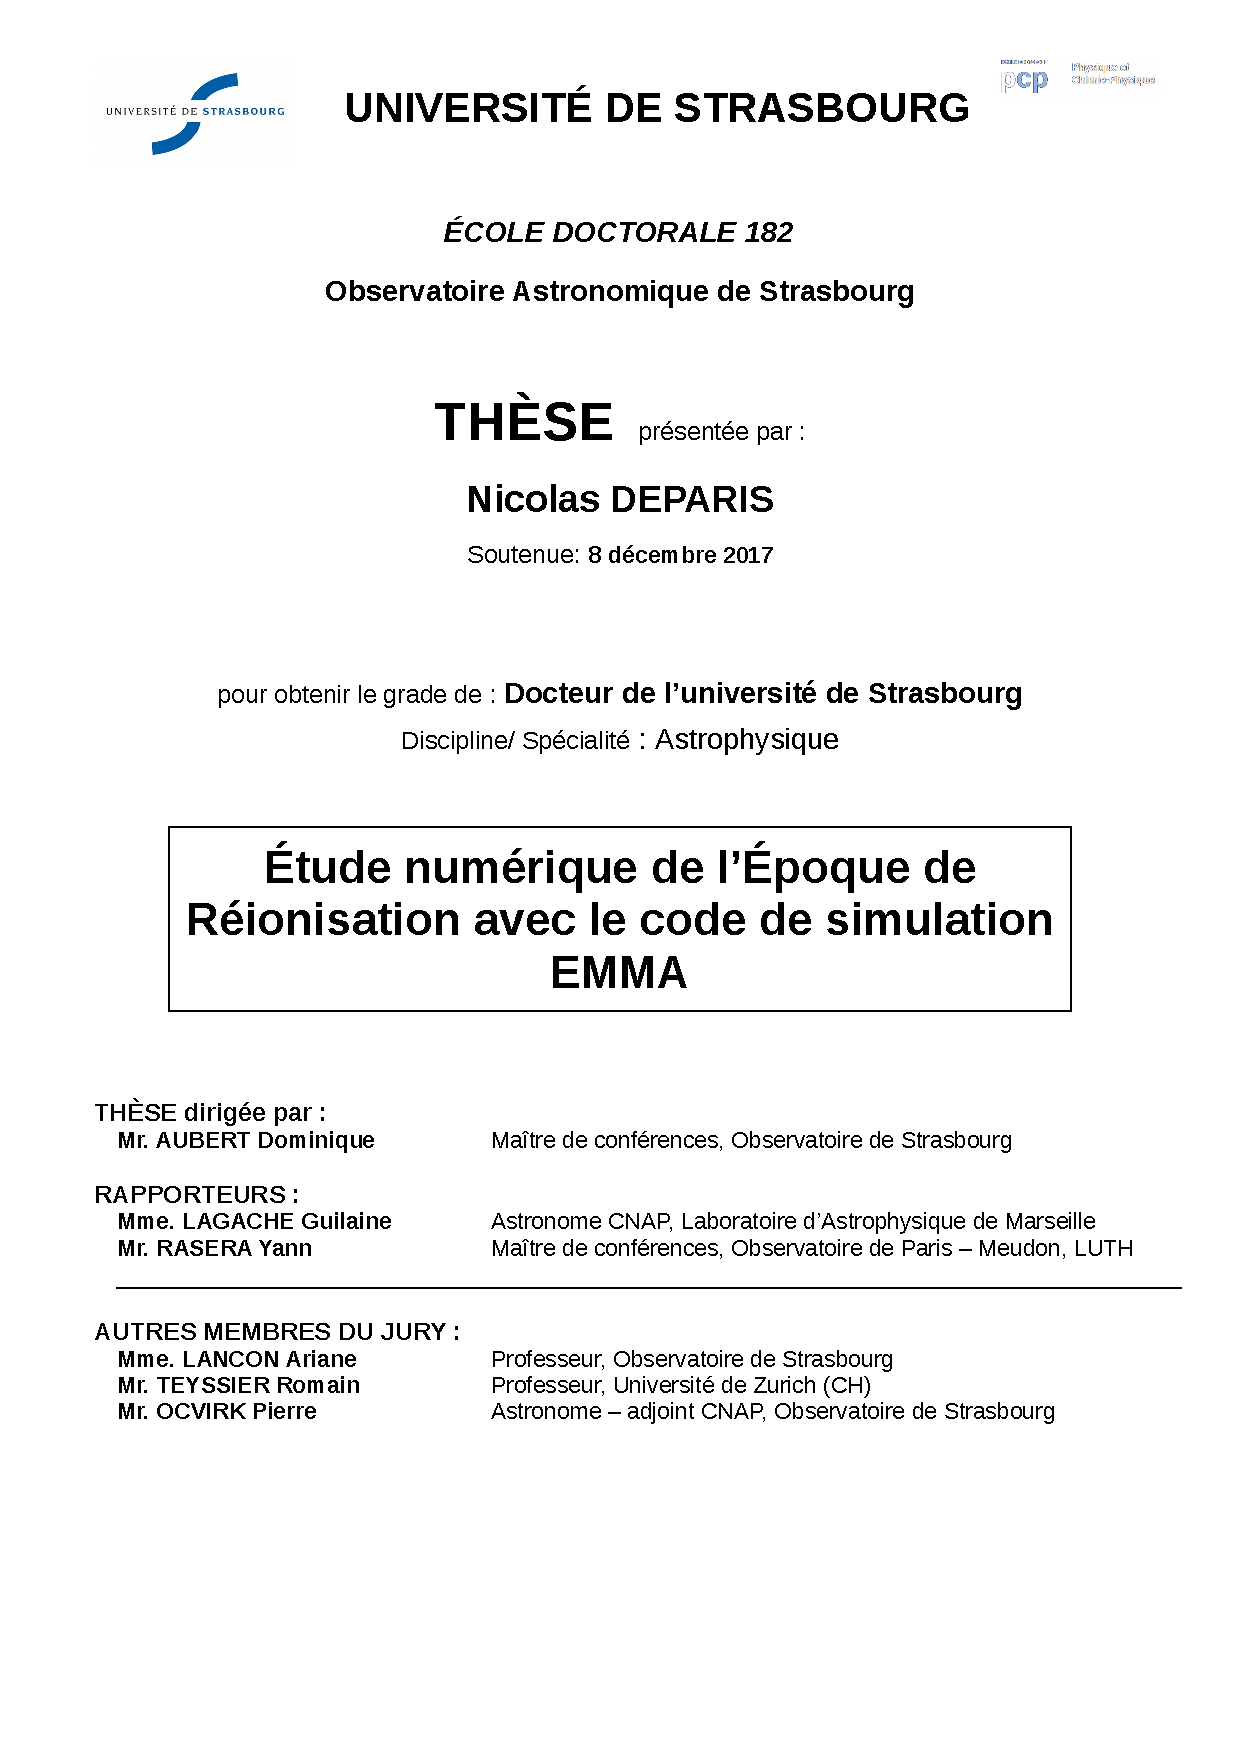
\includepdf{FrontBackmatter/couverture/1ere.pdf} 

%%*******************************************************
% Little Dirty Titlepage
%*******************************************************
\thispagestyle{empty}
%\pdfbookmark[1]{Titel}{title}
%*******************************************************
\begin{center}
    \spacedlowsmallcaps{\myName} \\ \medskip                        

    \begingroup
        \color{Maroon}\spacedallcaps{\myTitle}
    \endgroup
\end{center}        

%*******************************************************
% Titlepage
%*******************************************************
\begin{titlepage}
    % if you want the titlepage to be centered, uncomment and fine-tune the line below (KOMA classes environment)
    \begin{addmargin}[-1cm]{-3cm}
    \begin{center}
        \large  

        \hfill

        \vfill

        \begingroup
            \color{Maroon}\spacedallcaps{\myTitle} \\ \bigskip
        \endgroup

        \spacedlowsmallcaps{\myName}

        \vfill

        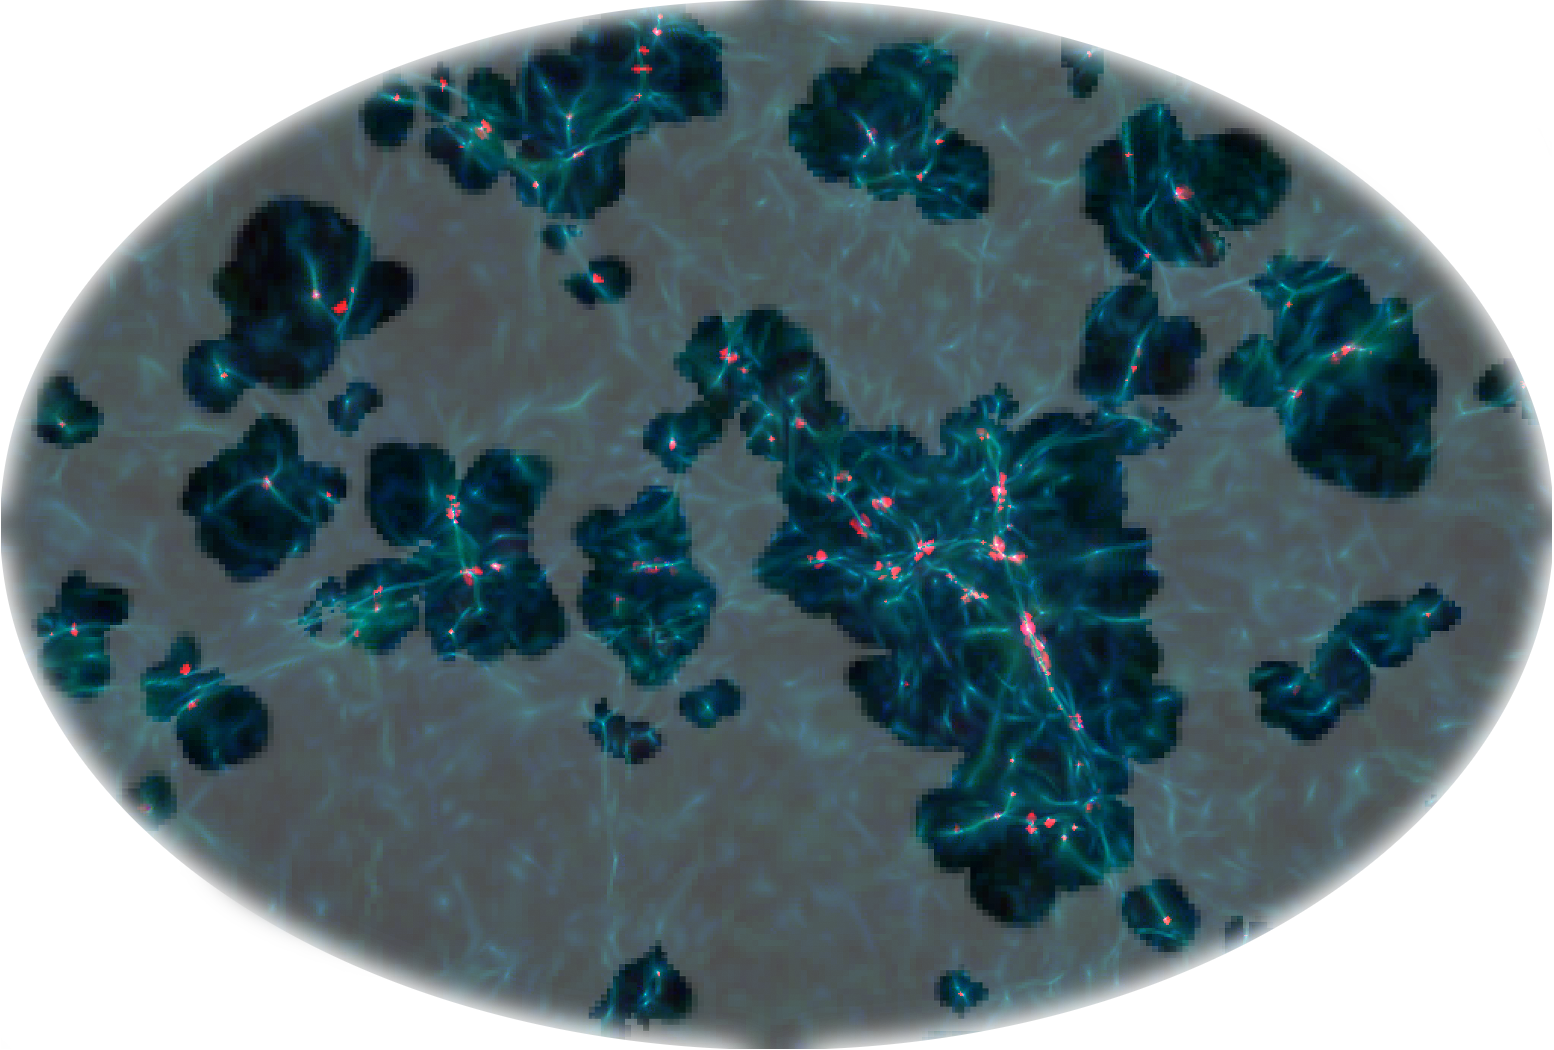
\includegraphics[width=12cm]{img/index.png} \\ \medskip

        \mySubtitle \\ \medskip   
        %\myDegree \\
        %\myDepartment \\                            
        %\myFaculty \\
        %\myUni \\ \bigskip

        \myTime\ -- \myVersion

        \vfill                      

    \end{center}  
  \end{addmargin}       
\end{titlepage}   
\thispagestyle{empty}

\hfill

\vfill

\noindent\myName: \textit{\myTitle,} %\mySubtitle, %\myDegree, 
%\textcopyright\ 
\myTime

%\bigskip
%
%\noindent\spacedlowsmallcaps{Supervisors}: \\
%\myProf \\
%\myOtherProf \\ 
%\mySupervisor
%
%\medskip
%
%\noindent\spacedlowsmallcaps{Location}: \\
%\myLocation
%
%\medskip
%
%\noindent\spacedlowsmallcaps{Time Frame}: \\
%\myTime

\cleardoublepage%*******************************************************
% Dedication
%*******************************************************
\thispagestyle{empty}
%\phantomsection 
\refstepcounter{dummy}
\pdfbookmark[1]{Dedication}{Dedication}

\vspace*{3cm}

\begin{center}
On fait la science avec des faits, comme on fait une maison avec des pierres; mais une accumulation de faits n'est pas plus une science qu'un tas de pierres n'est une maison. \\ \medskip
--- Henri Poincaré 
\end{center}

\vspace*{6cm}

\begin{flushright}
A Béatrice, Yann et Mariette.
\end{flushright}

%\cleardoublepage\include{FrontBackmatter/Foreword}
\cleardoublepage%*******************************************************
% Abstract
%*******************************************************
%\renewcommand{\abstractname}{Abstract}
\pdfbookmark[1]{Résumé}{Résumé}
\begingroup
\let\clearpage\relax
\let\cleardoublepage\relax
\let\cleardoublepage\relax

\chapter*{Résumé}
L’époque de réionisation (EoR) est une phase de grands changements qu’a subi l’Univers dans son premier milliard d’années. 
Suite à l’apparition des premières sources et à l’émission de photons énergétiques par ces dernières, l’hydrogène a été réionisé. 
Cette transition à eu un impact sur la formation des galaxies et leur contenance stellaire.

J’ai activement participé au développement d’EMMA, un code de simulation numérique aillant pour objectif d’étudier les processus a l’œuvre durant l’EoR. 
J’y ai développé et implémenté un modèle de formation et d’évolution stellaire et ces travaux ont contribué à la réalisation de "CoDa I AMR" une simulation dédiée à l’étude de l’EoR parmi les plus grandes réalisées à l’heure actuelle. 
J’ai également contribué au développement d’outils dédiés à l’exploration de simulations de ce type.

J’ai étudié la façon dont le rayonnement s’échappe des galaxies en fonction des paramètres du modèle stellaire, et montré qu'aux résolutions d’intérêt les supernovae peuvent augmenter la fraction de photons libérés.

J’ai également étudié la propagation des fronts d’ionisation et montré qu’il était possible de réduire la vitesse de la lumière par 3 (et ainsi diminuer le temps de calcul du transfert du rayonnement par 3), tout en conservant des résultats corrects.
CoDa I AMR a permis d'étudier le lien entre l'histoire de réionisation des halos et leurs masses actuelles.
Cette étude tend à confirmer l'hypothèse d'une réionisation précoce et interne du Groupe Local.


\vspace{0.5cm}

Mots clefs : Cosmologie, age sombres, réionisation, premières étoiles, méthodes numériques.
\vfill

\newpage

\begin{otherlanguage}{english}
\pdfbookmark[1]{Abstract}{Abstract}
\chapter*{Abstract}
The epoch of reionization (EoR) is a phase of big changes in the first billion years of the Universe history. After the apparition of the first stars and the emission of energetic radiation by thoses ones, the hydrogen was reionized. This transition has an impact on the galaxies formations.

I was part of the development team of EMMA, a numerical simulation code who aimed to study the  processes happening during the EoR. I developed and implement a stellar formation and evolution model. These works contributed to the realisation of "CoDa I AMR" one of the biggest simulation dedicated to the study of the EoR yet. I contribute to the development of a tool dedicated to the exploration of this kind of simulations.

I study how the radiation escaped the galaxies as a function of the parameters of the stellar model, and showed that supernovae could increase the ratio of escaping photon.

I also studied the ionization fronts propagation and showed that the speed of light could be reduced by a factor 3 (and then divide the computational cost of the radiative transfer by 3), while keeping corrects results.
CoDa I AMR was used to study the link between reionization histories and presents halos masses.
This study tends to confirm the hypothesis of an early and internal reionization of the Local Group.

\vspace{0.5cm}

Keywords : Cosmology, dark ages, reionization, first stars, numerical methods
\end{otherlanguage}

\endgroup			

\vfill





%\cleardoublepage%*******************************************************
% Publications
%*******************************************************
\pdfbookmark[1]{Publications}{publications}
\chapter*{Publications}\graffito{This is just an early --~and currently ugly~-- test!}
This might come in handy for PhD theses: some ideas and figures have appeared previously in the following publications:

%\noindent Put your publications from the thesis here. The packages \texttt{multibib} or \texttt{bibtopic} etc. can be used to handle multiple different bibliographies in your document.

\begin{refsection}[ownpubs]
    \small
    \nocite{*} % is local to to the enclosing refsection
    \printbibliography[heading=none]
\end{refsection}

\emph{Attention}: This requires a separate run of \texttt{bibtex} for your \texttt{refsection}, \eg, \texttt{ClassicThesis1-blx} for this file. You might also use \texttt{biber} as the backend for \texttt{biblatex}. See also \url{http://tex.stackexchange.com/questions/128196/problem-with-refsection}.
\cleardoublepage%*******************************************************
% Acknowledgments
%*******************************************************
\pdfbookmark[1]{Acknowledgments}{acknowledgments}

%\begin{flushright}{\slshape    
%    We have seen that computer programming is an art, \\ 
%    because it applies accumulated knowledge to the world, \\ 
%    because it requires skill and ingenuity, and especially \\
%    because it produces objects of beauty.} \\ \medskip
%    --- \defcitealias{knuth:1974}{Donald E. Knuth}\citetalias{knuth:1974} \citep{knuth:1974}
%\end{flushright}



\bigskip

\begingroup
\let\clearpage\relax
\let\cleardoublepage\relax
\let\cleardoublepage\relax
\chapter*{Acknowledgments}
Put your acknowledgments here.

Many thanks to everybody who already sent me a postcard!

Regarding the typography and other help, many thanks go to Marco 
Kuhlmann, Philipp Lehman, Lothar Schlesier, Jim Young, Lorenzo 
Pantieri and Enrico Gregorio\footnote{Members of GuIT (Gruppo 
Italiano Utilizzatori di \TeX\ e \LaTeX )}, J\"org Sommer, 
Joachim K\"ostler, Daniel Gottschlag, Denis Aydin, Paride 
Legovini, Steffen Prochnow, Nicolas Repp, Hinrich Harms, 
 Roland Winkler, Jörg Weber, Henri Menke, Claus Lahiri, 
 Clemens Niederberger, Stefano Bragaglia, Jörn Hees, 
 and the whole \LaTeX-community for support, ideas and 
 some great software.

\bigskip

\noindent\emph{Regarding \mLyX}: The \mLyX\ port was intially done by 
\emph{Nicholas Mariette} in March 2009 and continued by 
\emph{Ivo Pletikosi\'c} in 2011. Thank you very much for your 
work and for the contributions to the original style.


\endgroup




\pagestyle{scrheadings}
\cleardoublepage%*******************************************************
% Table of Contents
%*******************************************************
%\phantomsection
\refstepcounter{dummy}
\pdfbookmark[1]{\contentsname}{tableofcontents}
\setcounter{tocdepth}{2} % <-- 2 includes up to subsections in the ToC
\setcounter{secnumdepth}{3} % <-- 3 numbers up to subsubsections
\manualmark
\markboth{\spacedlowsmallcaps{\contentsname}}{\spacedlowsmallcaps{\contentsname}}
\tableofcontents 
\automark[section]{chapter}
\renewcommand{\chaptermark}[1]{\markboth{\spacedlowsmallcaps{#1}}{\spacedlowsmallcaps{#1}}}
\renewcommand{\sectionmark}[1]{\markright{\thesection\enspace\spacedlowsmallcaps{#1}}}
%*******************************************************
% List of Figures and of the Tables
%*******************************************************
\clearpage

\begingroup 
    \let\clearpage\relax
    \let\cleardoublepage\relax
    \let\cleardoublepage\relax
    %*******************************************************
    % List of Figures
    %*******************************************************    
    %\phantomsection 
    \refstepcounter{dummy}
    %\addcontentsline{toc}{chapter}{\listfigurename}
    \pdfbookmark[1]{\listfigurename}{lof}
    \listoffigures

    \vspace{8ex}

    %*******************************************************
    % List of Tables
    %*******************************************************
    %\phantomsection 
    \refstepcounter{dummy}
    %\addcontentsline{toc}{chapter}{\listtablename}
    \pdfbookmark[1]{\listtablename}{lot}
    \listoftables
        
    \vspace{8ex}
%   \newpage
    
    %*******************************************************
    % List of Listings
    %*******************************************************      
      %\phantomsection 
    \refstepcounter{dummy}
    %\addcontentsline{toc}{chapter}{\lstlistlistingname}
    \pdfbookmark[1]{\lstlistlistingname}{lol}
    \lstlistoflistings 

    \vspace{8ex}
       
    %*******************************************************
    % Acronyms
    %*******************************************************    
    \phantomsection 
    \refstepcounter{dummy}
    \pdfbookmark[1]{Acronymes}{Acronymes}
    \markboth{\spacedlowsmallcaps{Acronymes}}{\spacedlowsmallcaps{Acronymes}}
    \chapter*{Acronymes}
    \begin{acronym}[UMLX]
    \acro{AMR}{Adaptive Mesh Refinement}
	\acro{EoR}{Epoch of Reionization}
	\acro{DM}{Dark Matter}
	\acro{CIC}{Cloud In Cell} 
	\acro{SFR}{Star Formation Rate} 
	\acro{SFH}{Star Formation History} 
	\acro{IGM}{InterGalactic Medium} 
	\acro{UV}{UltraViolet} 
	\acro{IMF}{Initial Mass Function} 
	\acro{CRTA}{Coarse Radiative Transport Approximation} 
	\acro{DMP}{Dark Matter Particles} 
	\acro{IC}{Initial Condition} 
	\acro{OTSA}{On The Spot Approximation} 
    \acro{API}{Application Programming Interface}
    \acro{SPH}{Smooth Particle Hydrodynamic}
    \acro{GPU}{Graphical Processing Unit}
    \acro{CPU}{Central Processing Unit}
    \acro{RSLA}{Reduced Speed of Light Approximation}
    \acro{FOF}{Friend Of Friend}
    \acro{FOV}{Field Of View}
    \acro{FPS}{Frame Per Second}
    \acro{CMB}{Cosmic Microwave Background}
    \acro{RGB}{Red Green Blue}
    \acro{HDD}{Hard Drive Disk}
    \acro{SSD}{Solid State Drive}
    \acro{MUSCL}{Monotonic Upstream-Centered Scheme for Conservation Laws}
    \acro{HMF}{Halo Mass Function}
    \acro{GMF}{Galaxy Mass Function}
    \end{acronym}
\endgroup

%********************************************************************
% Mainmatter
%*******************************************************
\cleardoublepage\pagenumbering{arabic}
%\setcounter{page}{90}
% use \cleardoublepage here to avoid problems with pdfbookmark
\cleardoublepage

%
\chapter*{Avant-Propos}

\begin{flushright}{\slshape    
	Une civilisation sans la science \\
	c'est aussi absurde qu'un poisson sans bicyclette.} \\ \medskip 
	--- Pierre Desproges
\end{flushright}

%\begin{itemize}
%\item la révolution industrielle
%\item migration vers les villes (50\% de la population mondiale depuis pas longtemps)
%\item déconnexion de la terre a cause du béton
%\item déconnexion du ciel a cause des éclairages publique
%\item étudier l'astrophysique est essentiel pour que l'Homme reste humble et considère sa place dans l'univers pour ne pas courir a sa perte.
%\end{itemize}

De nombreuses cosmologies ont vues le jours au fil des siècles et des peuples.
La question de la place de l'Humanité dans l'Univers a toujours été centrale et au cœur des préoccupations de toutes les civilisations.
%Toutes ont en commun 

Il fut un temps ou l'Homme n'avait d'autre choix que de cultiver les champs le jour et vivre dans l'obscurité la nuit.
Il existait un lien fort entre ce qui se passait sur terre (Humanité vient de Humus après tout) et dans le ciel.
Il ne pouvait que constater le ciel étoilé et se poser la question de la provenance des lueurs qui remplissent la voûte céleste.

L’absence de lumière a toujours créer une peur de l'inconnu, cette fameuse peur du noir.
Depuis le XIX ème siècle et la revolution industrielle, il est devenu possible de s'affranchir de la nuit.
Et nous ne nous en sommes pas privé.

Nous vivons dans un monde ou plus de la moitié de la population mondiale vie dans des villes ou l'obscurité n'a pas sa place.
L’éclairage publique agis comme un écran qui nous bloque la vue du ciel, et par la même occasion inhibe cette sensation de vertige que l'on peu ressentir en le regardant.

Cette migration urbaine a aussi pour conséquence de nous couper du lien a la terre
Les villes sont presque intégralement étanchéifier par du béton.

L'étude de la cosmologie et sa vulgarisation est une nécessité si l'on veux retrouver une certaine humilité vis a vis de notre seul et unique lieu de vie.




\begin{flushright}{\slshape    
	You devellop an instant global consciousess, \\
	a people orientation,\\
	an intense dissatisfaction with the state of the world,\\
	and a compulsion to do something about it.\\
	From out there on the moon, internationnal politic look so petty. \\
	You want to grab a politician by the scuff of the neck\\
	and drag him a quarter of a million mile out and say: \\
	'Look at that you son of a bitch'\\ \medskip 
	--- Edgar Mitchell Appolo 14 astronaut }
\end{flushright}
\chapter{Introduction}

%Besoin des simu car contraintes observationnelles sur IGM mais impact fort sur les galaxies pas le même timing, physique complexe il faut simulaer


D'une manière générale, la méthode scientifique repose sur 3 piliers: 
\begin{enumerate}
\item L'observation
\item La théorie
\item L'expérience
\end{enumerate}
L'astrophysique moderne n’échappe pas a cette règle.

\paragraph{L'observation} est le plus ancien des piliers, et constitue le point de départ de toute démarche scientifique.
Avant même de chercher a comprendre un sujet, il faut recueillir des informations a son sujet. %le regarder et l'analyser.
L'Homme a toujours regardé le ciel.
Contrairement aux autres discipline scientifique, le point de vue que nous avons sur notre sujet d'analyse est unique. 
Il nous est impossible de changer notre point de vue sur l'Univers.
Les techniques d'observations ont fait d’énormes progrès ces dernières années, mais observer ne suffit pas.


%Il celui sur lequel repose le plus de poids puisque tout en découle.
%De plus il est commun a toute les disciplines scientifique.
%Il n'est pas de science possible sans observation.


\paragraph{La théorie} est le deuxième de ces piliers.
%Lorsque l'on voit ces lumière sur la voûte céleste, nous sommes obligé de nous poser la question essentielle de leur provenance.
%Cette question mène a l'élaboration de diverse formulation tentant d'expliquer comment (et pourquoi) le ciel s'illumine la nuit.  
%Dans le cadre de l'étude de l'univers dans sont ensemble, cette théorie est nommée cosmologie et repose sur des concept mathématiques complexes
L'objectif est ensuite de réussir a donner un sens aux informations récoltées.
Au fil des siècles, diverses théories ont été élaborées pour expliquer le comportement de l'Univers observable.
La force d'une théorie est jugée sur sa capacité à faire des prédictions.

\paragraph{L'expérience} est le dernier pilier.
L'expérience a pour but de mettre a l’épreuve la théorie.
Il nous est impossible de d'effectuer des expériences sur l'univers, notre porté d'interaction est bien trop réduite.
%observation, modélisation et test de la théorie or en astro on ne peut pas tester directement donc on simule.
Pilier le plus récent il est sensé palier au problème des deux autres : l'impossibilité de changer de point de vue ou de tester les théories élaborées.
Ici sous entendue la simulation numérique, il est beaucoup plus récente et dépend grandement de la technologie.
C'est celui vers lequel j'ai choisis de me diriger.






Notre compréhension actuelle de l'univers s'inscrit dans le cadre du modèle standard de la cosmologie.
Ce modèle repose sur un univers non statique et en expansion, aillant une origine, le Bigbang.
A une époque, l'univers était extrêmement chaud et concentré, il n'y avait alors ni étoiles ni galaxies.
Mais en grandissant,  le plasma primordial s'est refroidit, les premiers atomes se sont formés lors de ce que l'on nomme la recombinaison, qui a mené a l'émission du fond diffus cosmologique.
L'univers était alors extrêmement homogène que ce soit en densité ou en température, mais cette homogénéité n'était pas parfaite.
S'en suit une période ou les in-homogénéités primordiales se sont effondrées sur elles même du fait de la gravité.
Puis ces in-homogénéités sont devenues suffisamment dense pour former les première étoiles.
Le matériaux disponible pour leurs formations était alors abondant.
On pense que ces étoiles étaient beaucoup plus massives, et donc beaucoup plus énergétique que les étoiles observées actuellement.
Ces étoiles ont émis un rayonnement suffisamment énergétique pour séparer les électrons et les protons lies au moment de la recombinaison.
L'univers c'est alors retrouvé une nouvelle fois dans un état majoritairement ionisé. 
C'est cette transition entre un univers neutre et froid vers un univers chaud et ionisé que l'on appel l'époque de reionisation.
L'apparition des première sources lumineuse a eu un impact sur la façon dont la matière c'est organisé pour former les galaxies.
Il est probable que l'univers que l'on observe aujourd'hui, ai conservé les traces de cette grande époque de transition.

Une des difficulté a l'étude de la réionisation est l'époque a laquelle elle s'est produite, on considère actuellement qu'elle a eu lieu dans le premier milliard d'année de l'univers.
Or, pour observer l'univers jeune, il faut regarder loin, tellement loin que les meilleur télescopes actuel sont tut juste assez performant pour atteindre des époques aussi lointaines.
Il faudra attendre encore au moins un décennie avant la mise en place des prochaine générations de télescope assez puissant pour observer les environnement de formation de ces première sources lumineuses.

Mais en attendant, si les possibilité d'observation sont restreinte, nous pouvons utiliser d'autre méthodes pour tenter de comprendre les phénomènes en cours a cette époque.
Nous pouvons utiliser les simulations numériques.
En effet, les phénomènes en action pendant la réionisation sont nombreux et les modèles analytique trouvent leurs limites.
Avec l'avancée exponentielle des capacités de calculs, les ordinateurs se transforme petits a petit en véritable laboratoire pour les astrophysiciens.
A l'heure actuelle il commence a être possible de simuler l'effondrement de structures cosmologique, contenant du gaz, formant des étoiles qui émettent du rayonnement 

Ces simulations ont pour objectifs d'aider a comprendre les grandes questions en suspend dans l'étude de la réionisation.
Voici un aperçu de ces questions : 

\begin{itemize}
\item Quand sont apparue les premières sources lumineuses?
Nous verrons que les observations commencent a imposer certaines contraintes sur la fin de la reionization mais  nous n'avons actuellement qu'une vague idée de la durée du processus.

\item L'univers a t il été réionisé par quelques grosses sources très lumineuses ou par de nombreuses source moins énergétique.
La question reste ouverte de savoir si ce sont les quasars, sources relativement rare mais pouvant etre extrement energétique, ou les galaxies plus modeste mais beaucoup plus nombreuse.
Dans le cas ou lce serai les galaxies, serai ce les les plus légéres, extrement nombreuses ou les plus massives.

\item Comment ces premières génération d'étoiles ont influencé m'apparitions des suivante, et ont elles laissées des traces encores visible dans l'environement proches?

\end{itemize} 

En répondant a certaine de ces questions, les simulations numeriques prépare les futures mission d'observation.
En etudiant au prealable ce que l'on cherche a  observer, on a plus de chance d'observer au bon endroit et de la bonne facon.


Au stade actuel de notre compréhension de l'univers, les simulations numériques ont a la fois de très belles réussites mais souffres également de 

\subsection*{La réionisation}
Le dernier grand changement que l'univers a subit date de son premier milliard d'années.
L'apparition des premières étoiles a transformé l'Univers alors froid et sombre en un univers chaud et inondé de lumière.
Cette transition est due a l'effondrement gravitationnel du gaz qui a permit, par endroits, une élévation de densité et de température suffisante pour réamorcer des réactions de fusion thermonucléaire.
Il s'agit de la première génération d'étoiles.
Le matériaux disponible pour leurs formations était alors abondant.
On pense que ces étoiles étaient beaucoup plus massives, et donc beaucoup plus énergétique que les étoiles observées actuellement.
Cette première génération à émis un fort rayonnement ultraviolet qui a grandement impacté le milieu environnant, en le chauffant par effet thermique et en le déplacant par effet de pression de radiation.
De plus, a la fin de leur vie, ces étoiles massives ont explosées en supernovae, effectuant alors un puissant chauffage ainsi qu'un fort brassage du gaz.
En changeant la configuration du milieu, ces premières étoiles ont modelées les lieux d'apparition des générations suivantes et donc la distribution de matière observée aujourd'hui.
La vitesse de la lumière étant finie, il fallut un certain temps pour celle ci puisse atteindre tous les recoins de l'univers. Il est estimé aujourd'hui que les premières étoiles sont apparues alors que l'univers était âgé d'environ 300 millions d'années. Il fallut alors 700 millions d'années supplémentaires pour que le rayonnement atteigne tout ses recoins, situant donc la fin de la période de  réionisation à milliard d'années après le Big Bang.

\subsection*{Les simulation numeriques}
Pour étudier des phénomènes aussi fortement couplés que ceux considérés dans le cas de l'époque de réionisation, il est nécessaire d'avoir recours à des simulations numérique. 
Le but de ces simulations est de reproduire les observations sur la distribution de matière dans l'Univers.

Les premières simulations cosmologiques ne considéraient l'évolution que de la composante non collisionnelle de la matière, ie la matière noire.
Comme la matière noire constituent la masse la plus abondante de l'Univers, ces simulation permettent de suivre l'évolution de la distribution de matière sur les grandes échelles. 
Mais par essence la matière noire est une matière invisible. 
Il manquait donc une compossante importante : la matière visible, les barrions.

Le calcul de l'hydrodynamique du gaz fut alors introduit, puis avec lui les premiers modèles de formation stellaire apparurent.
Mais la communauté a vite été confronté a un important problème: le gaz refroidissait trop.
Ce qui avait pour conséquence qu'il s'effondrait sur lui même trop rapidement et formait trop d'étoiles.
Pour palier a ce problème, il fut proposé d'injecter de l'énergie dans les endroits les plus dense.
Cette énergie, introduite par les supernovae, permet de chauffer le gaz et ralentis son effondrement. 

%Depuis très récemment, une troisième physique est devenue  dans les simulations l'influence de la radiation sur le milieu est également prise en compte.
Aujourd'hui, l'intérêt est porté sur l'introduction d'une nouvelle physique, celle du rayonnement.
Le rayonnement émit par les étoiles, va changer les propriétés physico-chimique et thermique du gaz qui les environnent et ainsi modeler les lieux d\'apparitions des générations future d'étoiles


\subsection*{Le groupe local}
Le groupe local est un ensemble de quelques dizaines de galaxies, dont les principales représentantes sont la Voie Lactée et notre voisine Andromède.
Il s'agit de notre environnement galactique proche.
Ce qui le rend facilement observable.
L'observation de cet environnement nous fournis des informations essentielles sur la cosmologie de l'Univers.

Plus la precision des observations augmente, plus il est nécessaire d'avoir des simulations résolues disposant de toutes la physique nécessaire pur expliquer globalement les échelles considérées.
Les premières simulations de matière noires ont permit d'expliquer les observations réalisées sur la distribution de la matière aux grandes échelles.
Lorsque les capacité de calcul se sont révélées suffisantes pour explorer des résolutions plus fines, il est vite apparu un certain décalage entre simulation et observation. 
L'introduction de l'hydrodynamique a permis d'augmenter l'accord entre les deux, jusqu'à un second palier de résolution.
Aujourd'hui, l'introduction de la physique du rayonnement va certainement permette de diminuer encore les échelles auxquelles les simulations sont sont en accord avec les observations.
L'ordre de grandeur de ces échelles est celui de la taille du groupe local.

De plus, les échelles que l'on considère dans les simulations cosmologiques a rayonnement couplé se rapproche de plus en plus des échelles considérés dans les simulations d'évolution de galaxies.
L'objectif est ici de faire le lien entre la physique de l'univers dans son ensemble (la cosmologie) et de la physique régissant l'évolution de notre galaxie ou de sa voisine (la physique galactique).






\section{Organisation du manuscrit}
\begin{itemize}
\item Introduction au   cosmologique $\Lambda$ CDM et a la période de réionisation.
\item Présentation du model numérique (Papier emma)
\item Présentation du model d'étoiles (papier SN)
\item Présentation de l'outils des cartes de reionization (papier c)
\item 
\end{itemize}




J'ai travaillé au développement d'un code nommé \emma, capable de simuler l'évolution de la matière noire, du gaz et de la radiation a des échelles cosmologiques.
Il a pour principal objectif l'étude de la période de réionisation.
\emma\ est un code a maille adaptative (AMR) qui a la particularité d'être massivement parallèle et d'être accéléré par processeurs graphiques (\ac{GPU}).

La première partie de se manuscrit sera consacré a introduire le cadre théorique de cette étude et a présenter le modèle cosmologique actuel.
Je présenterai ensuite les grande lignes de \emma, qui permettront au lecteur de mieux appréhender les résultats obtenus a partir des simulations générées a partir de ce code.

Dans la première partie de ma thèse, ma tache principale a été d'implémenter un scénario de formation stellaire, ainsi qu'un modèle de feedback de supernovae.
D'une manière plus générale j'ai contribué à divers aspect du code, comme la gestion des paramètres utilisateur, l'écriture des données de sorties ou encore la documentation.
Je développe également une librairie d'analyse des fichiers générés par \emma.
J'ai également contribué au développement d'un code de visualisation et d'exploration de simulations astrophysique.

\subsection*{Mod\`ele de formation stellaire}
L'étude du rayonnement émis dans l'Univers, passe immanquablement par l'étude de la formation stellaire.
J'ai implémenté dans \emma, un modèle de transformation du gaz en particule stellaire.
Ce modèle est basé sur un critère de densité.
Lorsque, sous l'effet de la gravitation, une cellule devient suffisamment dense, celle ci est marquée comme étant autorisée a former des étoiles.
Ensuite, toute les cellules autorisées vont former une certaine quantité d'étoiles, fonction de l'état local de la cellule, et suivant une loi empirique issue de l'observation : la loi de Schmidt-Kennicutt.

Cette recette nécessite l'introduction de plusieurs paramètres libres.
Une partie importante du temps a été consacrée à la calibration de ces paramètres.

\subsection*{Mod\`ele de supernovae}

Historiquement, les modèles de formation stellaire se sont rapidement confronté à un problème majeur : ils n'arrivaient pas à reproduire les observations en terme de quantité d'étoiles crées.
Une réponse à ce problème fut l'introduction des supernovaes. 
Les explosions de supernovaes injectent une quantité non négligeable d'énergie dans le milieu environnant.
Cette énergie supplémentaire perturbe le milieu et régule la formation stellaire.

J'ai implémenté un modèle d'injection d'énergie dans le solveur hydrodynamique d'\emma.
Ce modèle considère deux types d'énergie. 
La première, thermique, va dissiper une certaine partie de l'énergie disponible dans le chauffage du gaz.
La seconde, cinétique, va mettre en mouvement le gaz environnant avec le reste de l'énergie.
Une certaine proportion de la masse de la particule stellaire est retournée dans le milieu. 
L'énergie totale et la masse des éjectas étant contrainte par un autre modèle, Starburst99.

De la même manière que précédemment, l'implémentation de ce modèle a introduit plusieurs paramètres libres qu'ils a fallut calibrer.






\part{Contexte}

\chapter{Introduction au modèle physique }\label{ch:introduction_physique}

\section{Les piliers}

L'intégralité de l'astrophysique repose sur 3 piliers:
\begin{enumerate}
\item L'observation
\item La théorie
\item La simulation
\end{enumerate}

lien avec la méthode scientifique de manière générale. observation, modélisation et test de la théorie or en astro on ne peut pas tester directement donc on simule.

L'observation est le premier de ces pilier. 
Il est le plus ancien et celui sur lequel repose le plus de poids.
L'Homme a toujours regardé le ciel.
De plus il est commun a toute les disciplines scientifique.
Il n'est pas de science possible sans observation.
La principale difficulté ici, est que le point de vue que nous avons sur l'Univers est unique. 
Il nous est impossible de le regarder sous un autre angle.

Vient ensuite la théorie.
Lorsque l'on voit ces lumière sur la voûte celleste, nous sommes obligé de nous poser la question essentielle de leur provenance.
Cette question mène a l'élaboration de diverse formulation tentant d'expliquer comment (et pourquoi) le ciel s'illumine la nuit.  
Dans le cadre de l'étude de l'univers dans sont ensemble, cette théorie est nommée cosmologie et repose sur des concept mathématiques complexes
Il nous est impossible de d'effectuer des expériences sur l'univers, notre porté d'interaction est bien trop réduite.

Enfin, le dernier pilier : la simulation.
Pilier le plus récent il est sensé palier au problème des deux autres : l'impossibilité de changer de point de vue ou de tester les théories élaborées.
Ici sous entendue la simulation numérique, il est beaucoup plus récente et dépend grandement de la technologie.
C'est celui vers lequel j'ai choisis de me diriger.

\section{observation -> Hubble}

découverte des galaxies\\
découverte de l'expansion de l'univers


\begin{figure}[bth]
        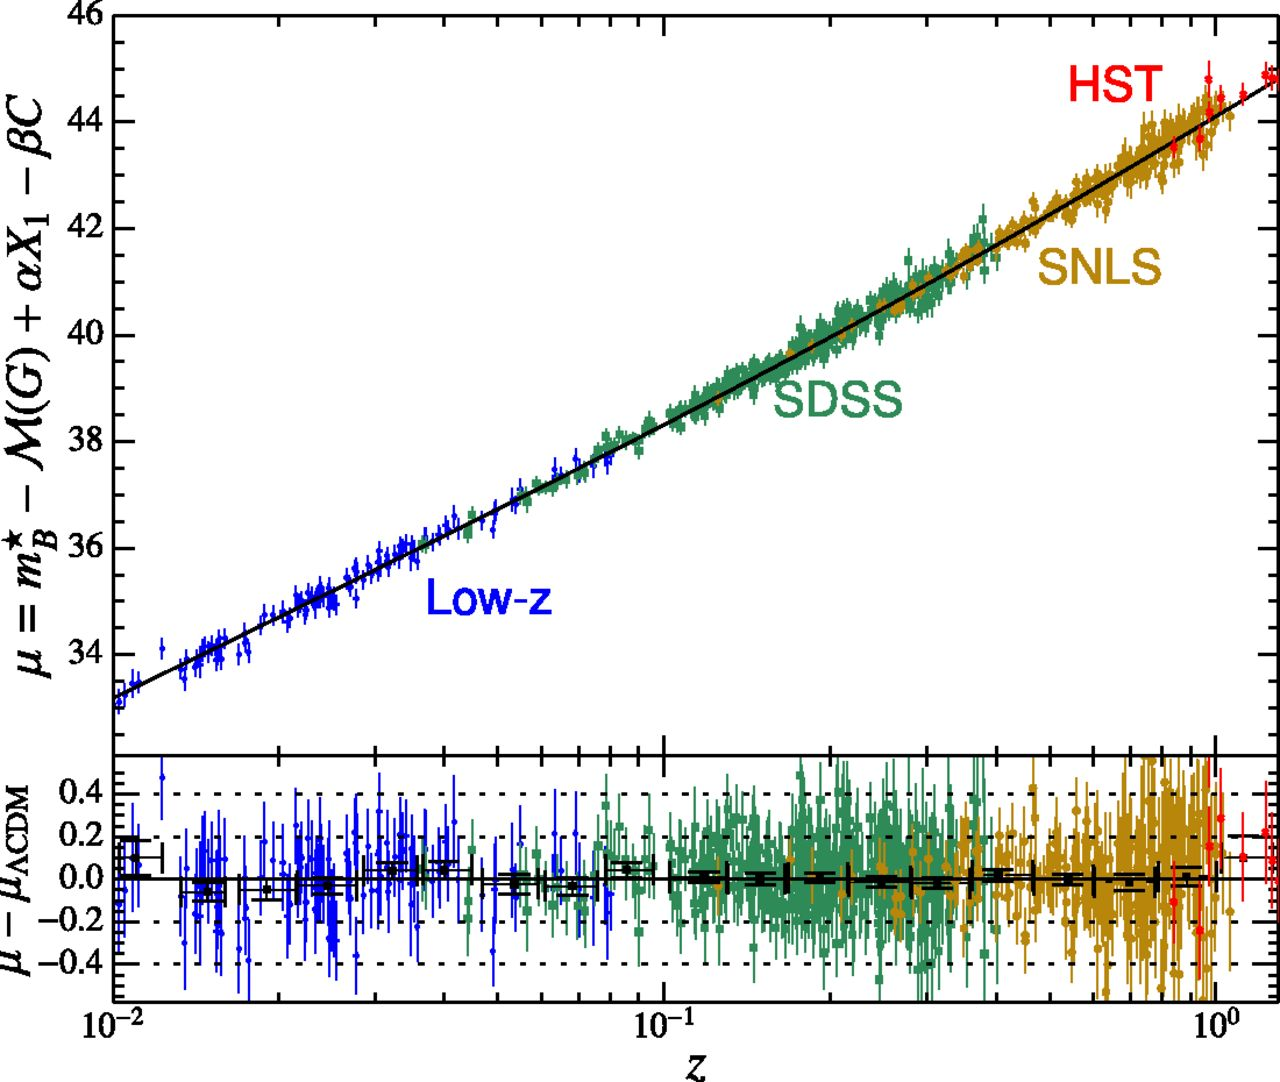
\includegraphics[width=.95\linewidth]{img/01/hubble_law.jpg} 
        \caption{Hubble law. 
%http://www.pnas.org/content/112/11/3173/F2.expansion.html
        Image ESO}
 		\label{fig:hubble_law}
\end{figure}

\begin{equation}
V = H_0 D
\end{equation}


\begin{figure}[bth]
        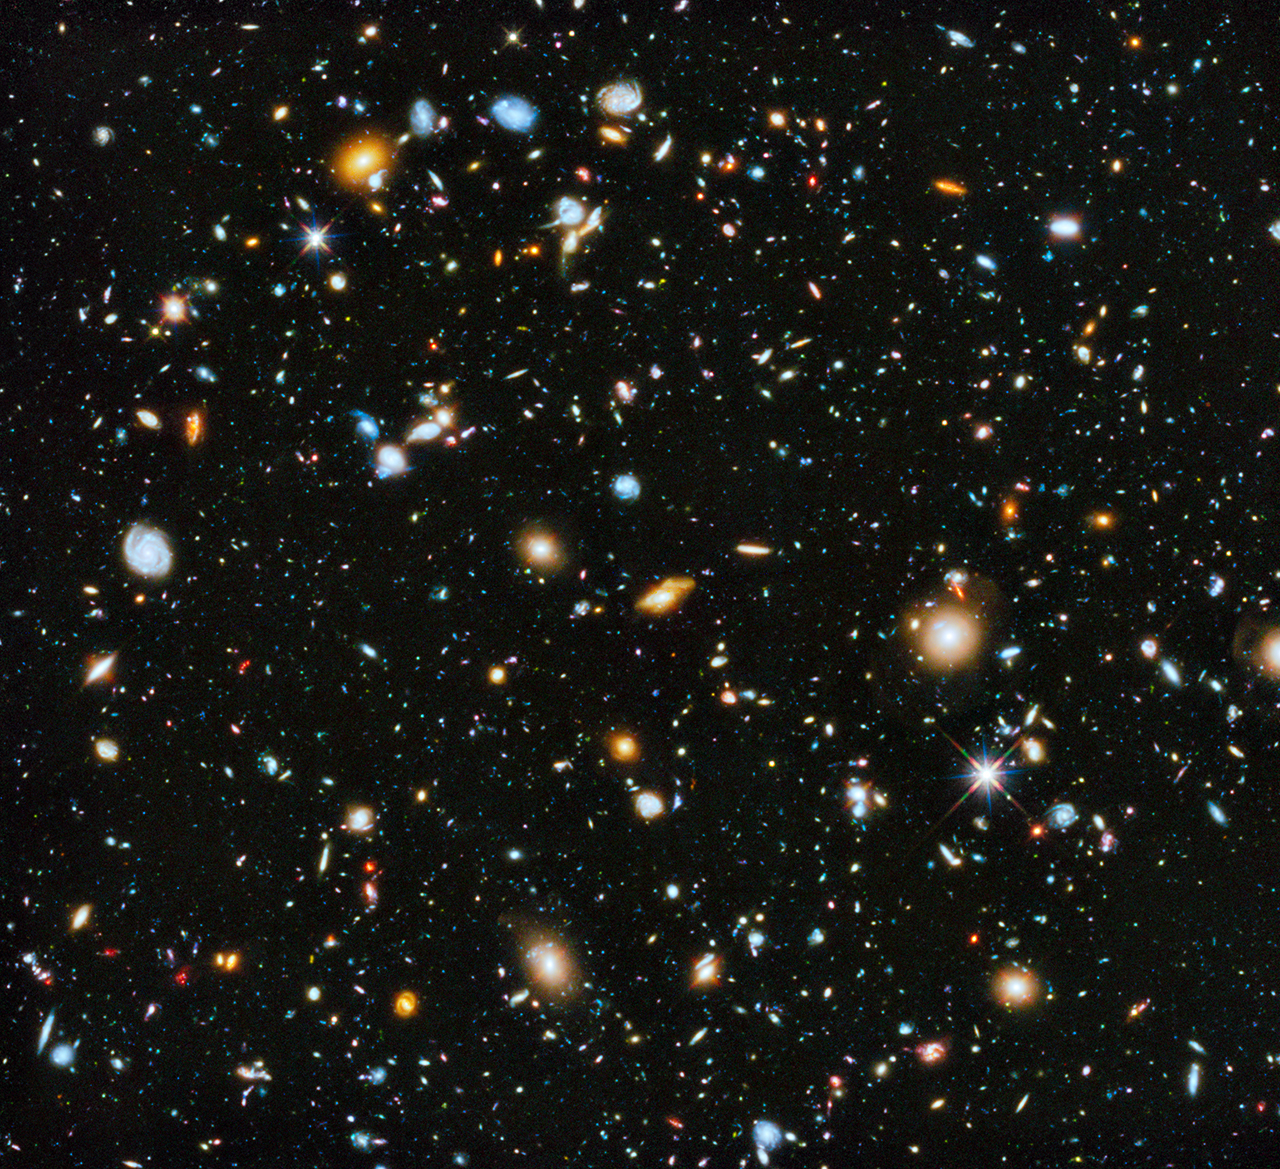
\includegraphics[width=.95\linewidth]{img/01/hudf.jpeg} 
        \caption{Hubble Ultra Deep Field 2014. 
        Image NASA}
 		\label{fig:hubbl_deep_field}
\end{figure}

\section{théorie - lCDM}

le big bang\\
l'inflation\\
la nucléosynthèse\\
le CMB\\
la reionization


\section{Le CMB}


\subsection{Observations}

Penzias et Willson

\subsection{Théorie}

surface de dernière diffusion


\subsection{Température}
Le cosmic Microwawe background se presente sous la forme du corp noir le plus parfait connus.
Fig. \ref{fig:cmb_thermal_spectrum}
T=2.73K


\begin{figure}[bth]
        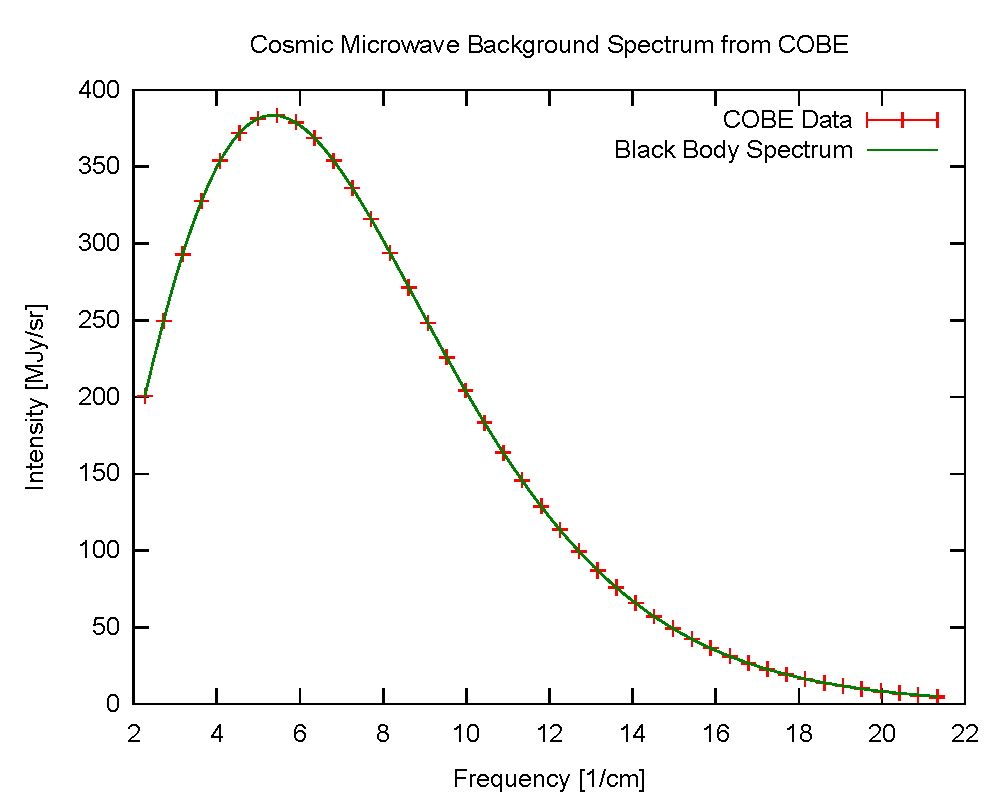
\includegraphics[width=.95\linewidth]{img/01/Cmbr.pdf} 
        \caption{Spectre thermique du CMB vue par le satellite Cosmic Background Explorer (COBE). 
        Image Wikipédia}
 		\label{fig:cmb_thermal_spectrum}
\end{figure}




\subsection{Spectre de puissance}

Le CMB n'est pas uniforme, il presente de tres faibles fluctuations (1e-5)qui nous renseigne sur l'etat de l'univers au moment de son emission.
Fig. \ref{fig:cmb_power_spectrum}

\begin{figure}[bth]
        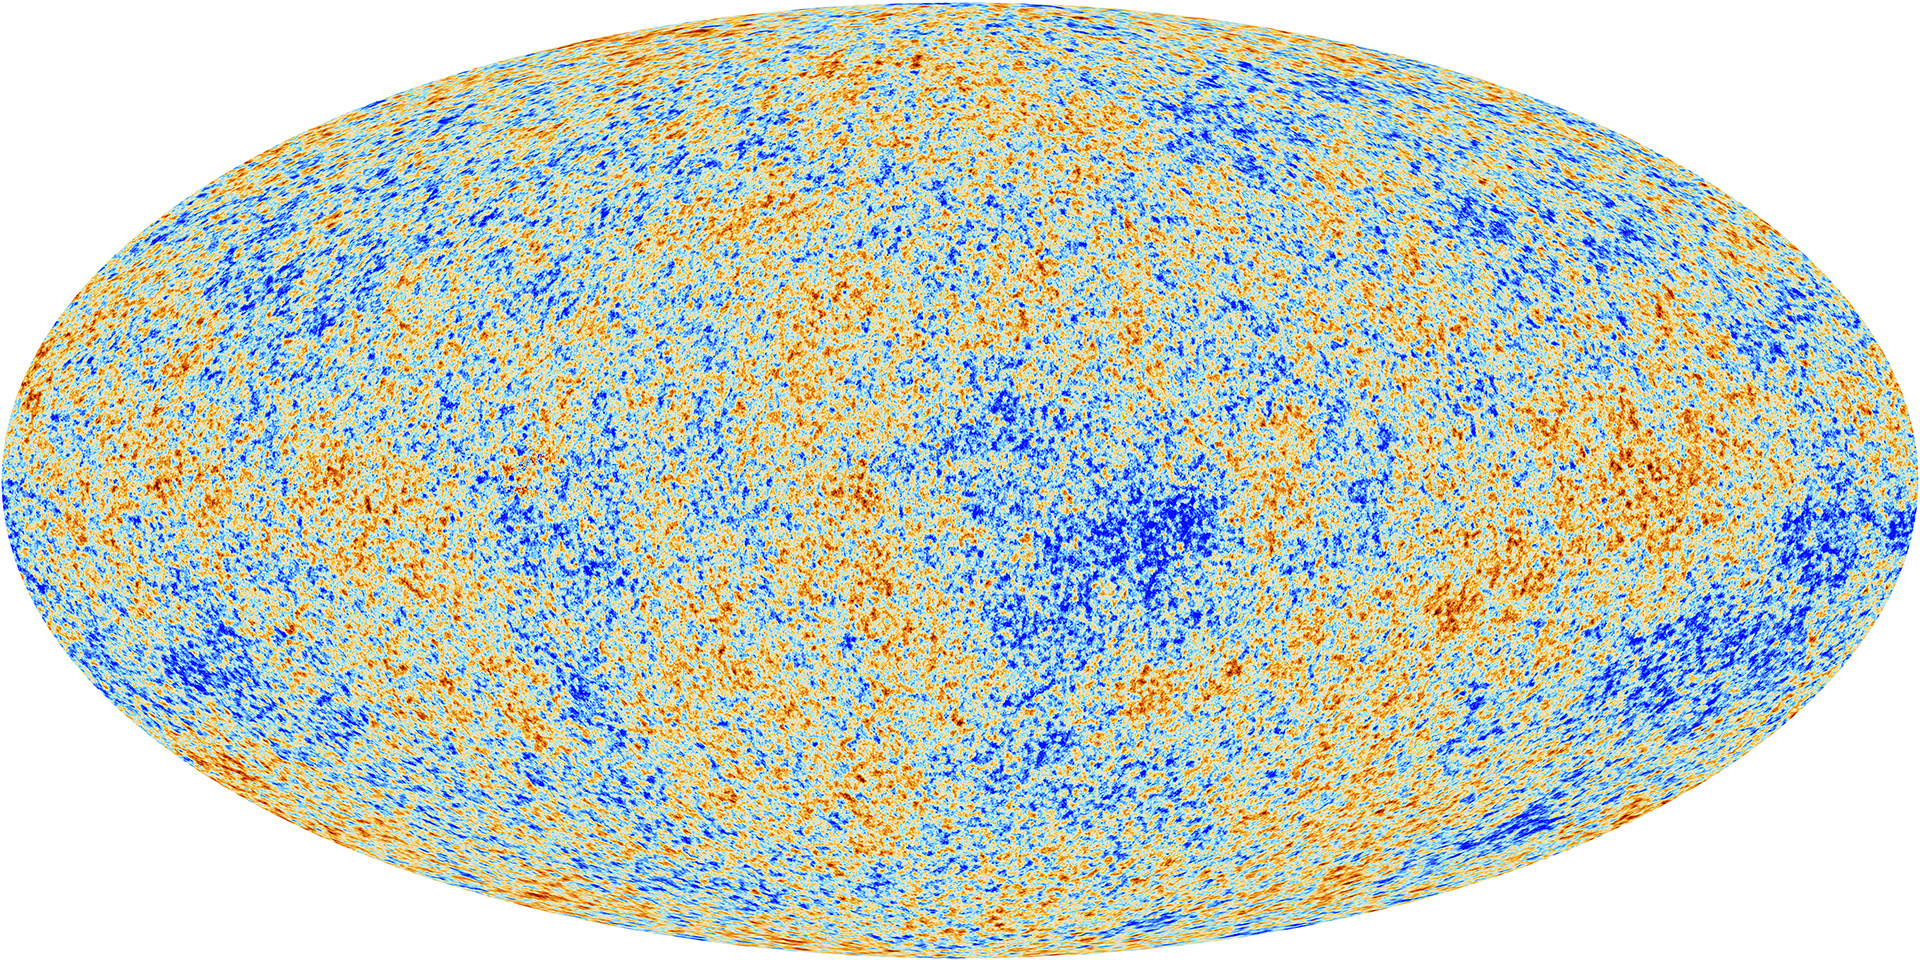
\includegraphics[width=.95\linewidth]{img/01/CMB.jpeg} 
        \caption{Les fluctuation du CMB vues par le satellite Planck. 
        Image ESA}
 		\label{fig:cmb}
\end{figure}


En decomposant ces fluctuations en harmoniques sphériques:
Fig\,\ref{fig:harmoniques_spheriques}

decomposition en multipoles
%https://www.physicsforums.com/threads/can-someone-explain-angular-power-spectrum.309483/
\begin{equation}
 \frac{\Delta T(\theta,\phi)}{T} = \sum_{l>0} \sum_{m=-l}^l a_{lm} Y(\theta,\phi)_{lm}
\end{equation}

avec : 

\begin{equation}
a_{lm}= \int d\Omega(\theta,\phi) \Delta T (\theta,\phi) Y(\theta,\phi)_{lm}
\end{equation}

\begin{figure}[bth]
        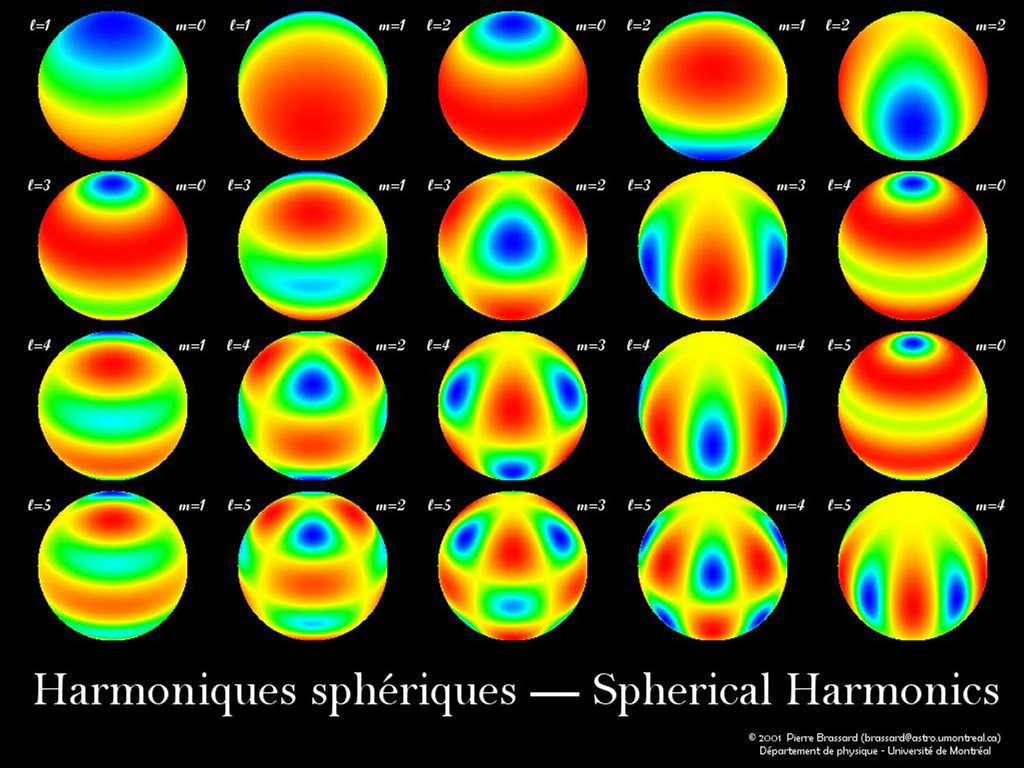
\includegraphics[width=.95\linewidth]{img/01/harmoniques_spheriques.jpeg} 
        \caption{
        représentation des $Y(\theta,\phi)_{lm}$
 Pierre Brassard, université de Montréal 
%Spectre thermique du CMB vue par le satellite Cosmic Background Explorer (COBE). 
        Image Wikipédia}
 		\label{fig:harmoniques_spheriques}
\end{figure}


\begin{equation}
C_l = \frac{1}{2l+1} \sum_{m=-l}^l a_{lm} a_{lm}^*
\end{equation}


Et finalement, on obtient le spectre de puissance:

\begin{equation}
D_l = \frac{l (l+1) C_l }{2 \pi} 
\end{equation}

représenté Fig.\,\ref{fig:cmb_power_spectrum}

\begin{figure}[bth]
        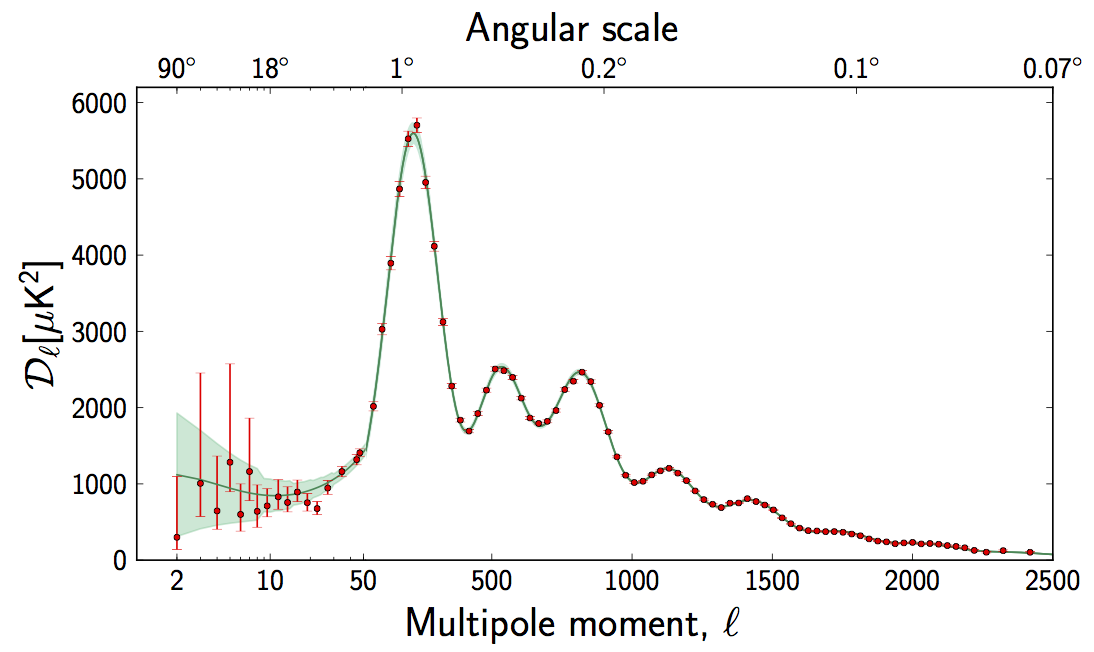
\includegraphics[width=.95\linewidth]{img/01/CMB_power_spectrum.png} 
        \caption{Spectre de puissance des fluctuation du CMB.
        Image ESA}
 		\label{fig:cmb_power_spectrum}
\end{figure}


\section{Le contenu de l'univers - (Théorie)}

Pour simuler l'univers, on a besoin de savoir ce qu'il contient. 
A partir du spectre de puissance, on peut déterminer les différentes composantes de l'univers (paramètres cosmologique).

univers infini, homogène, isotrope


%https://ned.ipac.caltech.edu/level5/Freedman2/Freed6.html


\begin{figure}[bth]
        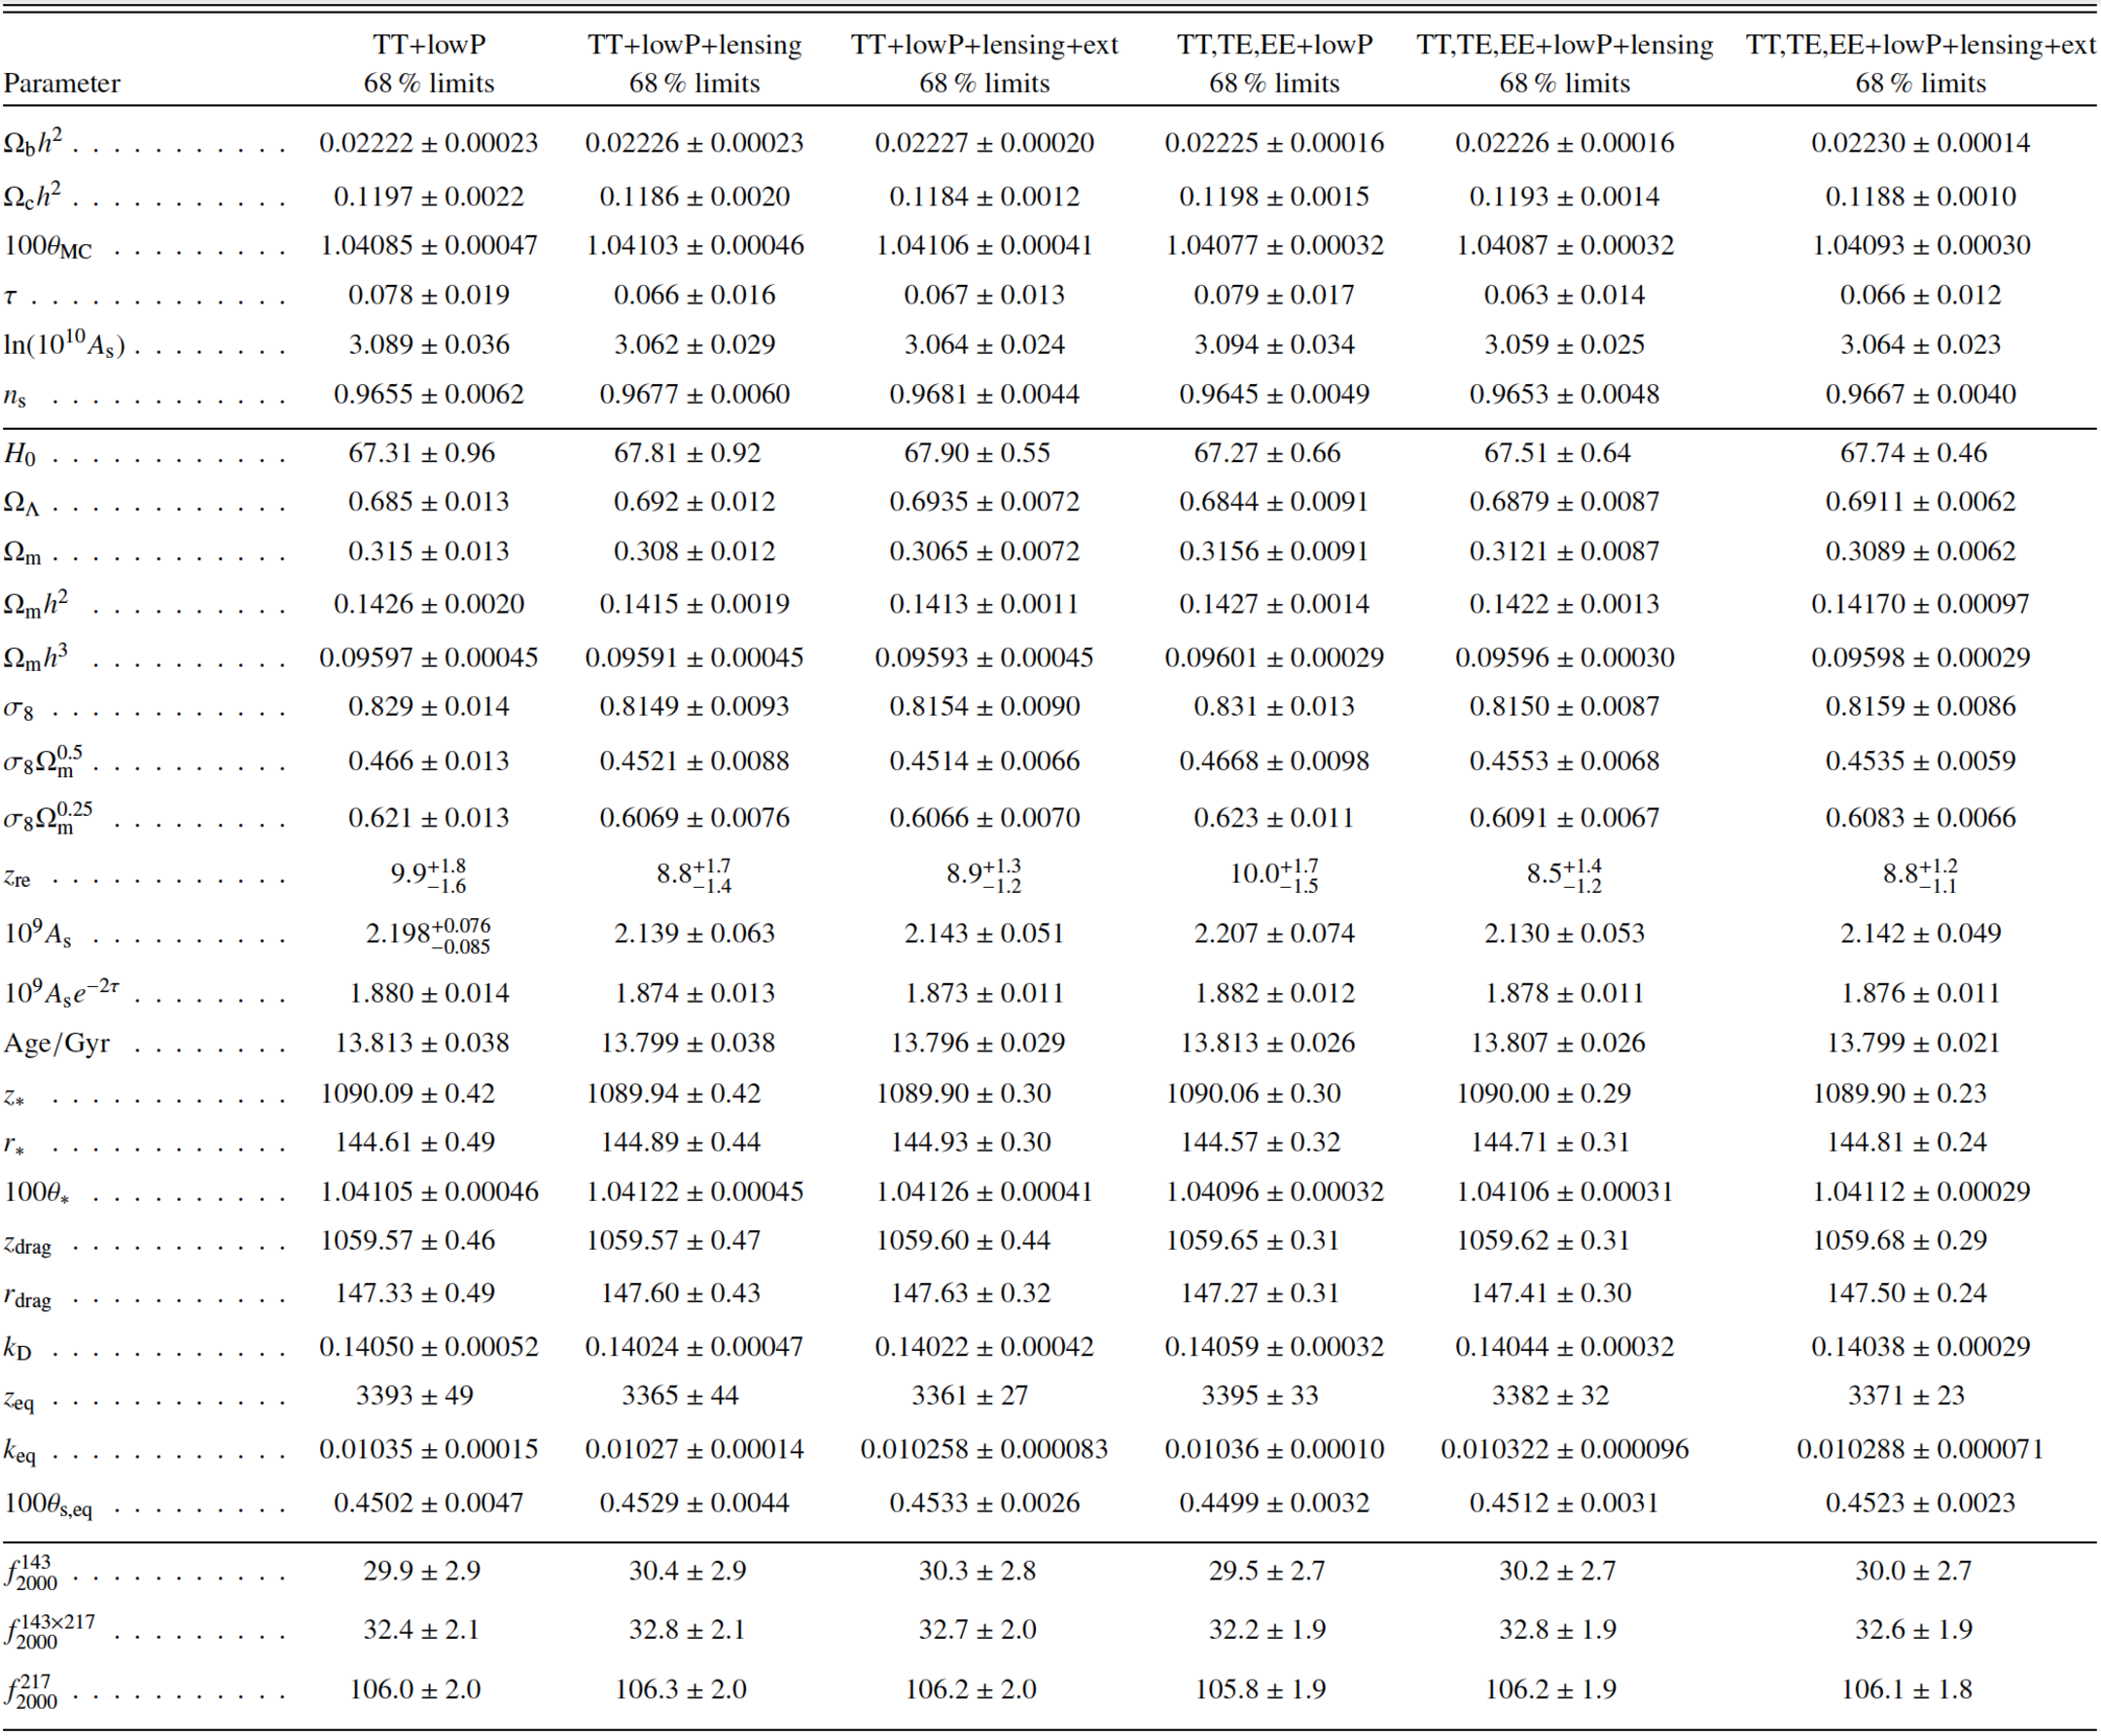
\includegraphics[width=.95\linewidth]{img/01/table_planck.pdf} 
        \caption{Determination des parametres cosmologiques par la colaboration Planck.}
 		\label{fig:planck_parameters}
\end{figure}

\citep{planck_collaboration_planck_2016}

\subsection{Energie noire}

echelle gigaparsec
Facteur d'expansion

\subsection{Matière noire}

echelle mega parsec
gouverne la gravité
non collisionnelle

\subsection{Baryon}

echelle kilo parsec
collisionnelle
interagit avec la radiation
La matière visible

\subsection{Radiation}

quasiment notre seul source d'information sur l'univers (plus vrai depuis les ondes gravitationnelles)
essentielle pour la reionization
seulement E>13.6 eV

\subsection{bilan}

plot en camembert avec les différents constituants

\section{Observation -> la reionization}

le manque d'observations

la difficulté des observations

les futures observations

Quelles sont les preuves de la réionisation?

\subsection{spectre de quasar}

tunnel gun peterson
\begin{figure}[bth]
        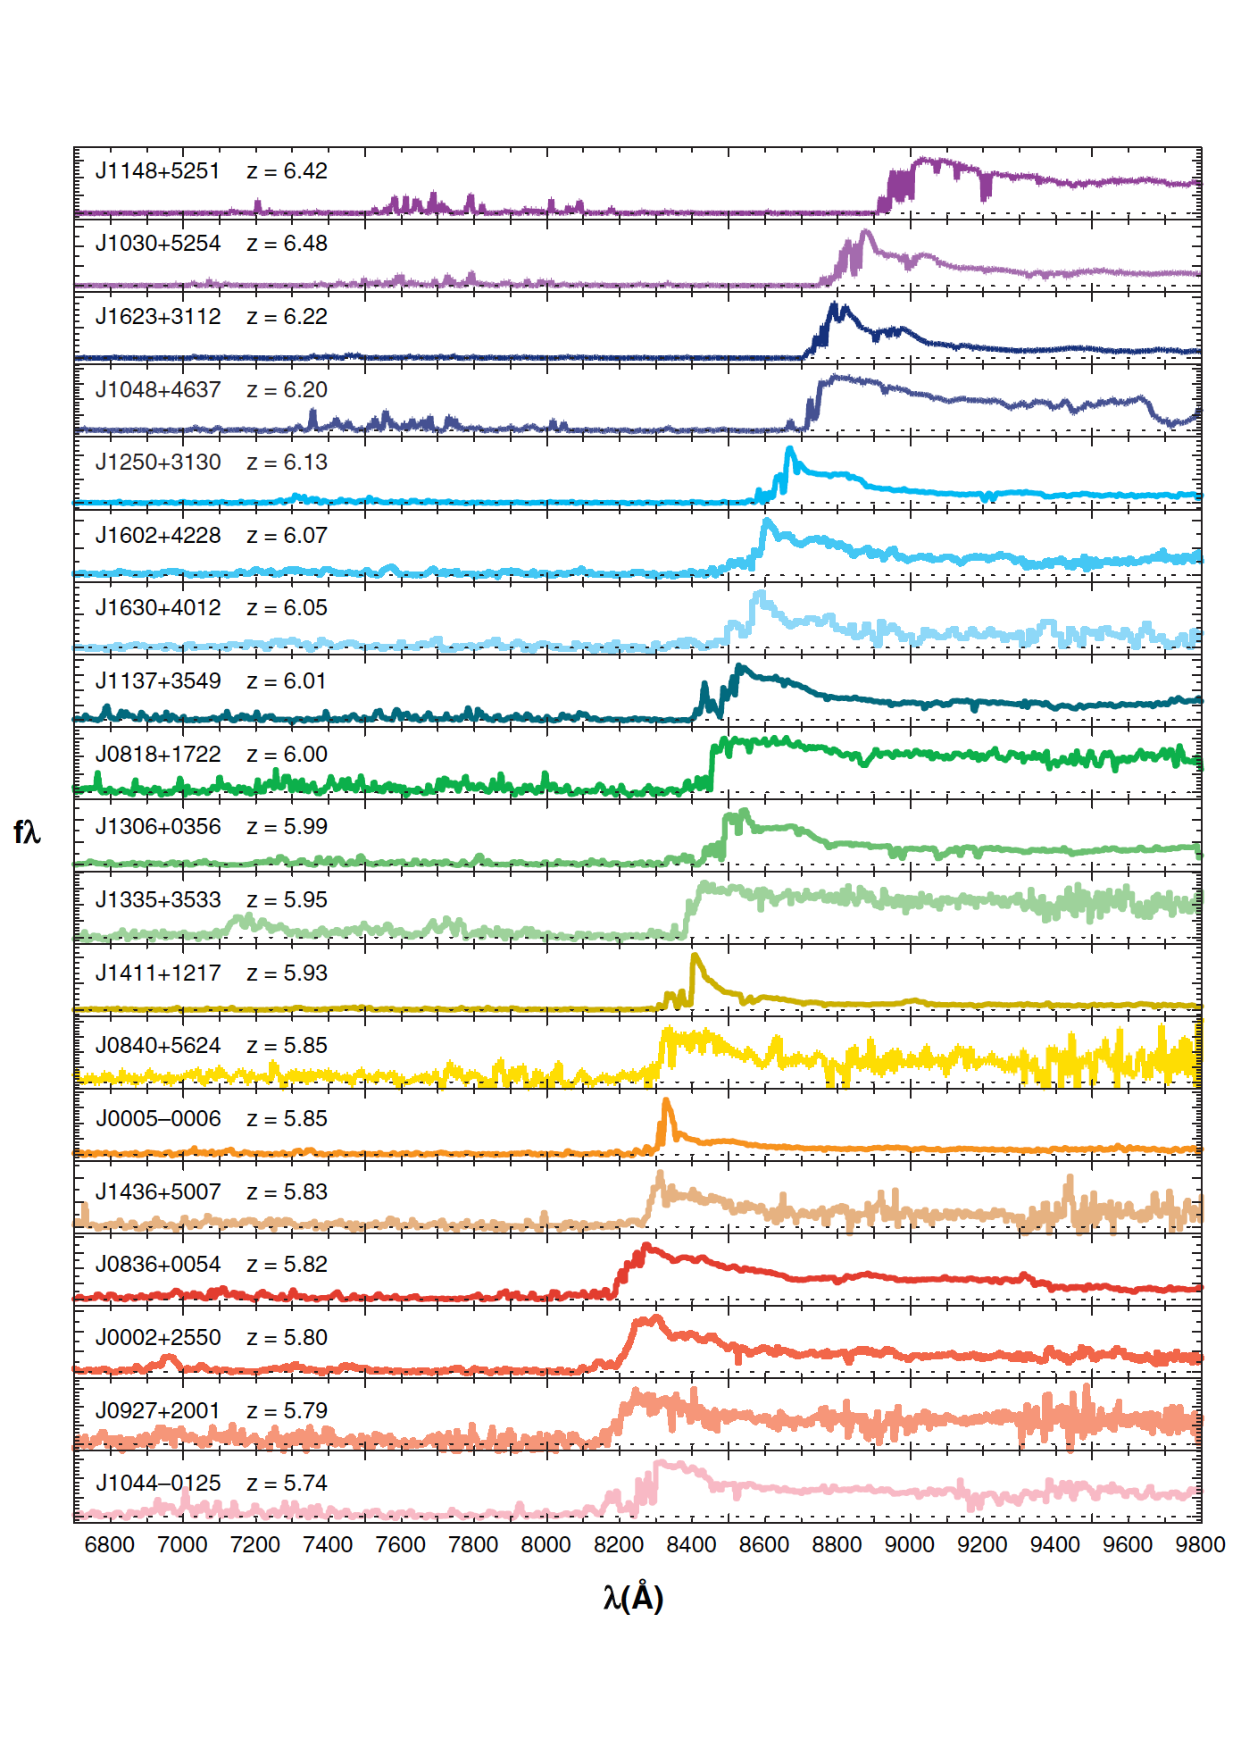
\includegraphics[width=.95\linewidth]{img/01/quasar_spectre.pdf} 
        \caption{Spectre de quasar a differents redshift presentant un tunnel gun peterson.
        Image fan et al.}
 		\label{fig:spectre_quasar}
\end{figure}

\subsection{Epaisseur optique lyman alpha}

\begin{figure}[bth]
        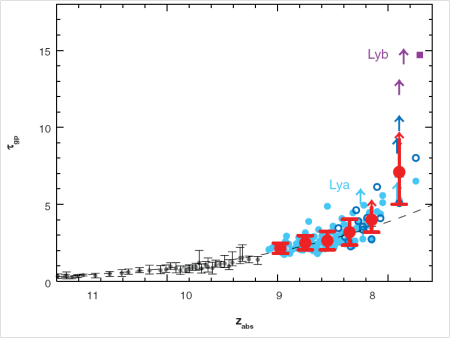
\includegraphics[width=.95\linewidth]{img/01/epaisseur_optique_quasar.png} 
        \caption{%https://ism2009.wordpress.com/2009/04/28/on-the-density-of-neutral-hydrogen-in-intergalactic-space/
		Epaisseur optique calculée a partir des spectres de quasar de la Fig\,\ref{fig:spectre_quasar}
        Image fan et al.}
 		\label{fig:spectre_quasar}
\end{figure}

\subsection{Epaisseur optique lyman alpha}

\begin{figure}[bth]
        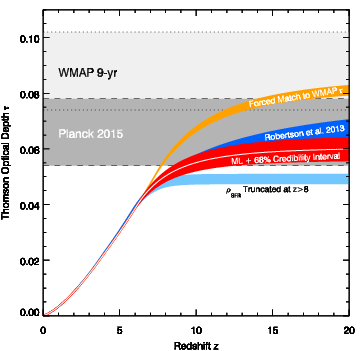
\includegraphics[width=.95\linewidth]{img/01/epaisseur_optique_thomson.png} 
        \caption{%https://inspirehep.net/record/1343310/plots
		Epaisseur optique Thomson
        Image Robertson et al.}
 		\label{fig:spectre_quasar}
\end{figure}



polarisation du CMB

ligne 21 cm

fonction de luminosité UV



\section{Théorie -> La reionization}

réionisation et non rayonnisation!

Qu'est ce que c'est?

fin des âges sombres
apparition des première sources de rayonnement
Pourquoi étudier la réionisation

Dernier processus impactant l'ensemble de l'univers.
Importance pour le "missing satellite problem"

\subsection{Sphère de Stromgren}


\subsection{les principales question en suspend de l'étude de la réionisation}

quand est ce arrivé?
quelles sont les sources? -> débat galaxies vs quasars
\begin{figure}[bth]
        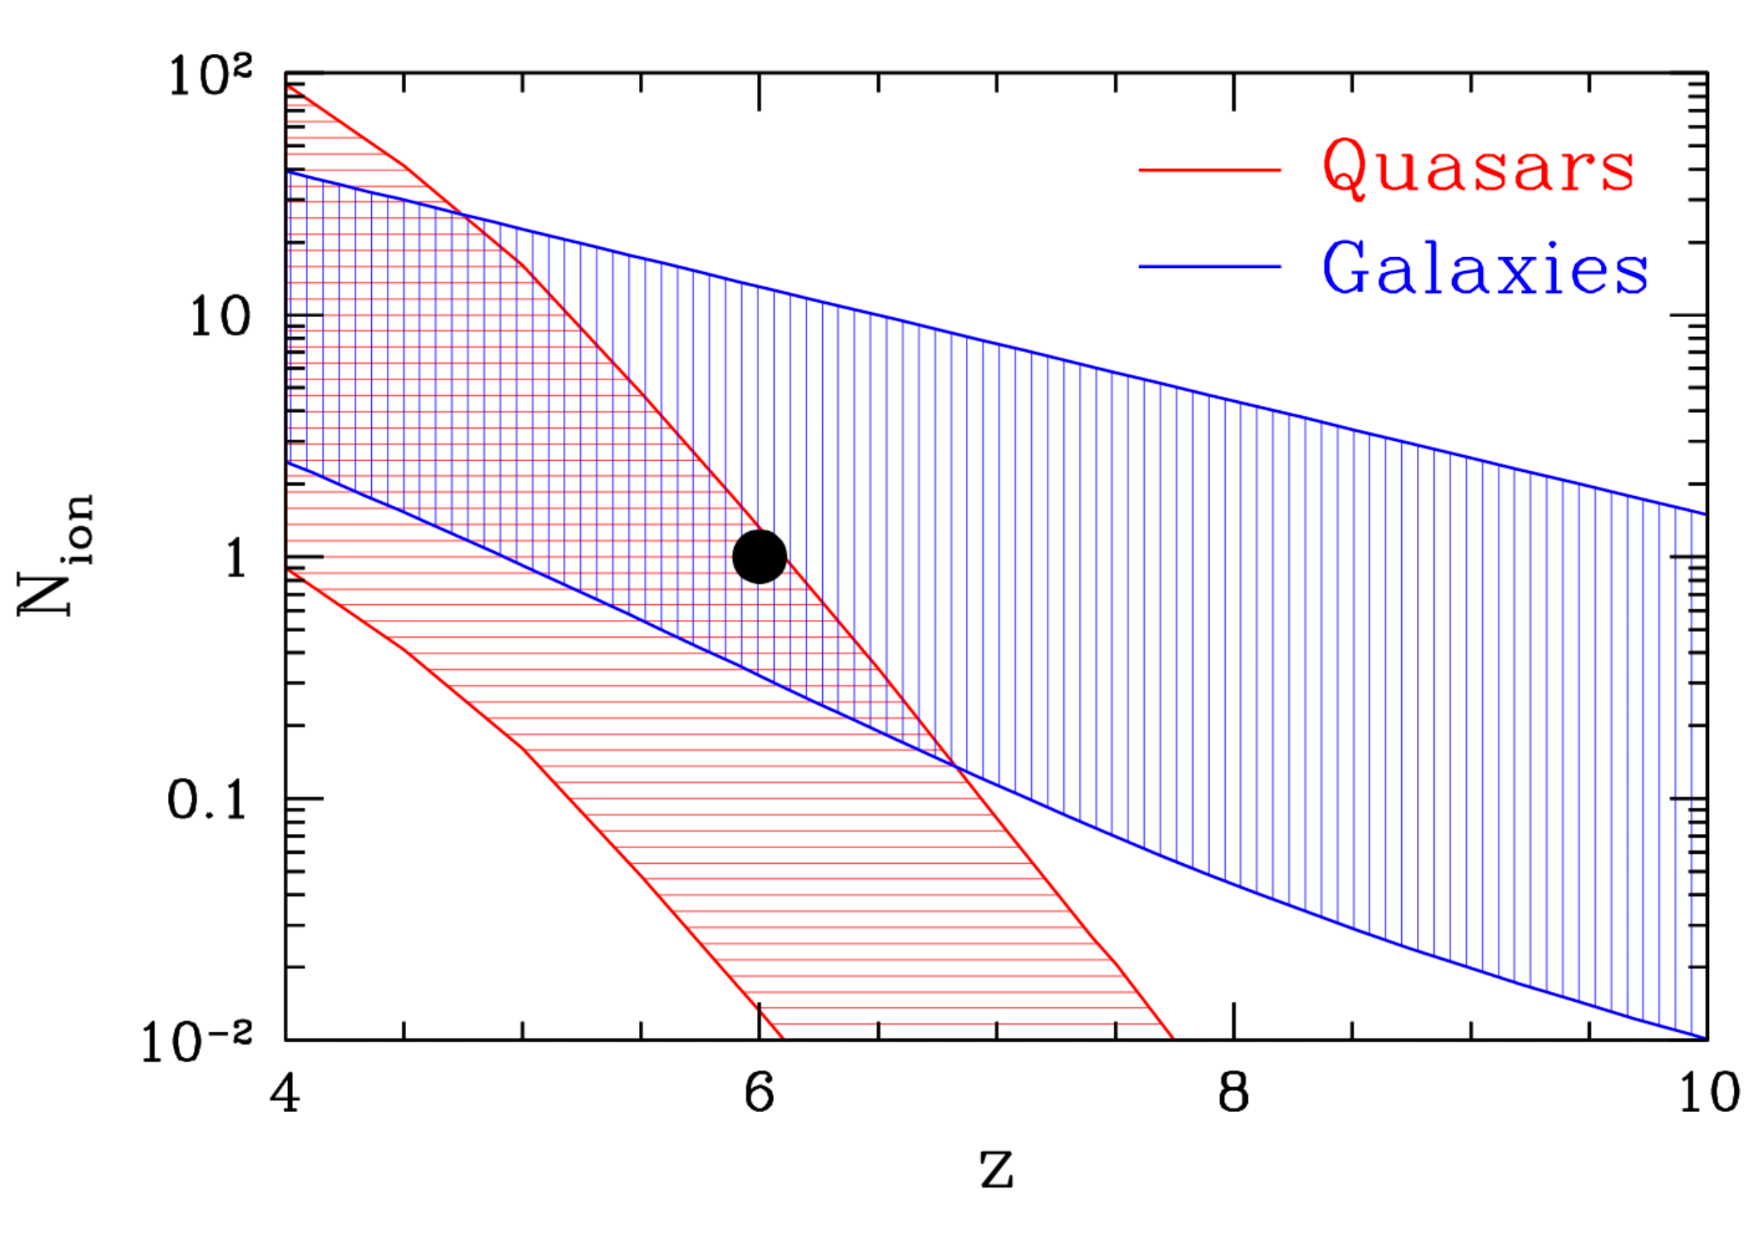
\includegraphics[width=.95\linewidth]{img/01/gal_AGN.pdf} 
        \caption{
        Budget de photons provenant des galaxies et des quasars qurant la reionization.
}
 		\label{fig:spectre_quasar}
\end{figure}

outlier dans l'épaisseur optique des quasars
Le groupe local ?



\chapter{La reionisation} 
\label{sec:introreio}
%réionisation et non rayonnisation!
%\section{Observation -> la reionization}
%%\section{Théorie -> La reionization}
%
%
%Qu'est ce que c'est?
%
%fin des âges sombres
%apparition des première sources de rayonnement
%Pourquoi étudier la réionisation
%
%Dernier processus impactant l'ensemble de l'univers.
%Importance pour le "missing satellite problem"
%%le manque d'observations
%%la difficulté des observations

Nous avons vu dans le chapitre précédent que lors de la recombinaison, l'Univers est passé d'un état globalement ionisé à un état globalement neutre.
%De cette transition, qui a eu lieu a environ 380000 ans après le Bigbang, en a résulté L’émission du CMB.
Suite a cette étape, l'univers était alors très homogène et ne disposait pas de source lumineuse, c'était les "ages sombres".

Sa dynamique était régie essentiellement par la lutte entre l'expansion et la gravitation et la compétition entre ces deux forces, couplée à de très légères perturbations a menée a l'effondrement de certaines certaines parties.
Il faudra alors attendre plusieurs centaine de million d'année pour voir apparaître des surdensité de gaz suffisamment compactes pour former les première étoiles.
Ces premières sources lumineuses ont émis un puissant rayonnement ionisant qui a a nouveau séparé les protons et les électron formé lors de la recombinaison.
Il a fallut encore plusieurs centaine de million d'année pour que les première sources de rayonnement soient suffisamment nombreuses pour que leurs photons remplissent l'univers, et le fasse passer d'un état majoritairement neutre, a un état a nouveau majoritairement ionisé. 
Cette transition s'appelle l’époque de la réionisation.

%à l'apparition des premières des premières étoiles.
%L'Univers va alors subir un changement d'état majeur, puisque le rayonnement énergétique des premières étoiles va de nouveau ioniser le gaz.
%C'est l'époque de la réionisation.

%Du fait que l'univers était neutre, le rayonnement n’était pas en mesure de se propager librement.
%A la suite de l'émission du fond diffus cosmologique, commence une période appelée "les ages sombres".
%L'Univers est alors composé de gaz froid soumis principalement à deux forces : la gravité et l'expansion de l'Univers.
%Ces étoiles ont émis du rayonnement suffisamment énergétique pour arracher les électrons du gaz environnant.



L'objectif de cette section est de présenter les grandes lignes des principes physique qui ont eu lieu durant cette période.
Je présenterai également quelques des preuve observationnelles qui confirme que la réionisation a bien eu lieu.
%Dans cette section, je vais présenter quelques unes des preuve observationnelles de la réionisation. 

%Une des difficultés de l’étude de la période de réionisation est que celle si a eu lieu tôt dans l'histoire de l'univers lors de son premier milliard d'années.
%Cette distance temporelle impose de regarder loin spatialement et donc de disposer de moyen observationnels important.
%Nous somme au balbutiement des observation de la réionisation.

\section{Principe général}

Lorsqu'une étoile se forme dans un environnement d'hydrogène neutre, son rayonnement va être capable d'ioniser l'hydrogène autour d'elle dans une zone définie.
Ces zones forment des bulles, et quand plusieurs bulles apparaissent proches les unes des autre, elles percollent pour en former un plus grande.
Ces région sont nommées régions HII et une grande partie de l'étude de l'époque de réionisation consiste à étudier leurs croissance.
Dans le but d’appréhender les principes de base à l’œuvre pendant la réionisation, nous allons commencer par nous placer dans un cas simple et idéal.

\subsection{Sphère de Strömgren}
\label{sec:stromgren}

Une source lumineuse ponctuelle apparaît instantanément dans un milieu infini, avec une densité et une température homogène et composé exclusivement d’hydrogène neutre.
Les questions sont alors : 
\begin{itemize}
\item Comment va évoluer l’état d'ionisation du gaz autour de cette source ?
\item Quelle région cette source va ioniser autour d'elle?
\end{itemize}

En considérant l'équilibre entre $\dot{N_\gamma}$ le nombre de photons ionisant émis par la source et le taux de recombinaison du milieu, \cite{stromgren_physical_1939} a exprimé l'évolution du rayon de la sphère ionisée $r_i(t)$:

\begin{equation}
\frac{dr_i(t)^3}{dt} = -n_H \alpha_B(T)r_i (t)^3 + \frac{3 \dot{N_\gamma} }{4 \pi n_H},
\end{equation}

où $\alpha_B(T)$ est le coefficient de recombinaison, fonction de la température et $n_H$ la densité d'hydrogène neutre.
La solution de cette équation est de la forme :

\begin{equation}
r(t) = r_s \left( 1 - e^{-t\cdot \alpha_B(T) n_H } \right)^{1/3}
\end{equation}

%
%\begin{equation}
%t_{rec} = \left( \alpha_B(T) n_H \right) ^{-1}
%\end{equation}

Le rayon de Strömgren est défini comme étant la solution stationnaire de cette équation:

\begin{equation}
r_s = \left( \frac{3 \dot{N_\gamma} }{4 \pi \alpha_B(T) n_H^2} \right)
\end{equation}

Nous voyons ici que connaissant l'émissivité de la source et la densité et température du milieu environnant, il est possible d'estimer la taille de sa région HII.

\subsection{Le cas non idéal}
Nous venons de voir un modèle théorique sensé représenter la croissance des régions HII.
En réalité : 
\begin{itemize}
\item les sources ne sont pas d'intensité constante. %Les étoiles évoluent et meurent, si il n'y a 
\item la densité n'est pas homogène,% (motif en papillon autour des filament)
\item les sources ne sont pas isolées,
\end{itemize}

%C'est ce dernier point qui va permettre a 
%l'Univers de réionise en entier car les sources sont nombreuses et c'est la percolation des régions HII des régions successives d'étoiles 

Se sont les générations successives d'étoiles et l'augmentation du taux de formation stellaire qui permet a l'Univers de reioniser en entier.
Les régions HII croissent de manière asymétrique en fonction de la géométrie du milieu, et forment des motifs en "papillons" autour des amas et des filaments.
La percolation de ces régions augmente petit a petit le taux d'ionisation de l'univers, jusqu'a ce qu'il ne reste plus que une fraction de neutre de l'ordre de $10^{-4}$.
Il est possible d'estimer l'évolution de la fraction d'hydrogène ionisé globale en utilisant :
\begin{equation}
\frac{dQ_{HII}}{dt} = \frac{\dot{N}_{ion}}{ <n_H>} - \frac{Q_{HII}}{t_{rec}},
\end{equation}

où, $\dot{N}_{ion}$  est le taux d'émission de photon ionisant et dépend du taux de formation stellaire et du profile d'emmisivité des sources.
%taux d'effondrement des structures.

\section{Preuves observationnelles}
\label{sec_contraintes_obs}

Dans cette section nous verrons quelles sont les principales observations montrant que la réionisation a effectivement eu lieu.

\subsection{Spectre de quasar et épaisseur optique Lyman alpha}

Historiquement, les spectres de quasar lointains ont été les premières preuves que l'Univers était fortement neutre dans le passé.
Les quasars sont des objets suffisamment brillants pour être observé à très grandes distance.
En 1965 il est observé \citep{1965ApJ...141.1295S} que le spectre des plus lointains d'entre eux présente une absorption caractéristique, appelée tunel Gun-Peterson \citep{1965ApJ...142.1633G}.
Avant de poursuivre, il est nécessaire  de revenir sur le spectre d’émission de l’hydrogène.

\subsubsection*{Raie Lyman alpha}

\begin{figure}
\centering
        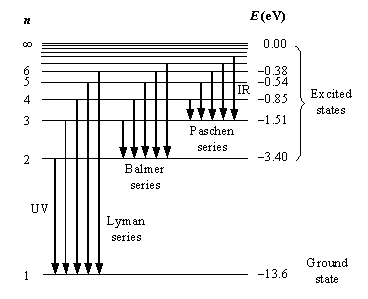
\includegraphics[width=.9\textwidth]{img/01/lyman.jpg} 
        \caption[Raies de l'hydrogène]{Changement de niveau d'énergie de l'atome d'hydrogène}
 		\label{fig:lyman}
\end{figure}

La série de Lyman correspond a la transition atomique menant au fondamental de l'atome d'hydrogène.
Il existe plusieurs série de transition autre que celle de Lyman (cf Fig. \ref{fig:lyman}) mais cette dernière est la plus énergétique et la plus fréquente, et donc la plus facile à détecter.
Il y a émission d'un photon Lyman-alpha pendant la transition de l'électron du premier état excité vers l’état fondamental (n2 -> n1).
L'énergie de cette transition est de 1216 $\AA$,  ce qui place l’émission dans l'Ultra Violet.
Réciproquement, la transition n1 vers n2 mène a l'absorption d'un photon Lyman-alpha.
C'est a dire que si un nuage de gaz neutre se trouve entre une source et l'observateur, le spectre réceptionné présentera une raie d'absorption à 1216 $\AA$.

\subsubsection*{Forêt Lyman alpha}

Maintenant considéreront des distances cosmologique entre la source et l'observateur.
Durant le parcours des photon, l'Univers aura subis une expansion et le spectre d'émission de la source sera redshifté.
Le spectre présentera des raie d’absorption à différents endroit suivant le moment de rencontre des différents nuages de gaz neutre.
C'est série de raies est très dense à haut redshift et est appelée forêt Lyman alpha.

\subsubsection*{Tunnel Gun Peterson}

Si nous considérons maintenant que la source est a l’intérieur d'une zone neutre, la série de raies absorbée ne sera plus discrète mais continue.
C'est ce continuum d’absorption que l'on nomme tunnel Gun-Peterson \cite{1965ApJ...141.1295S}

La figure \ref{fig:spectre_quasar} montre une série d'observations de spectres de quasars.
Ces spectres sont classés par redshift, et le tunnel GP des plus éloigné est particulièrement visible.

%Dans le cas de la reionisation, les sources sont des quasar.
%Les quasars sont des objets suffisamment brillants pour être observé a très grandes distance.
%Il est observé que plus leur redshift est important, plus leur foret lyman alpha est important.
%Les plus lointains d'entre eux présentent  un tunnel gun peterson.

\begin{figure}
        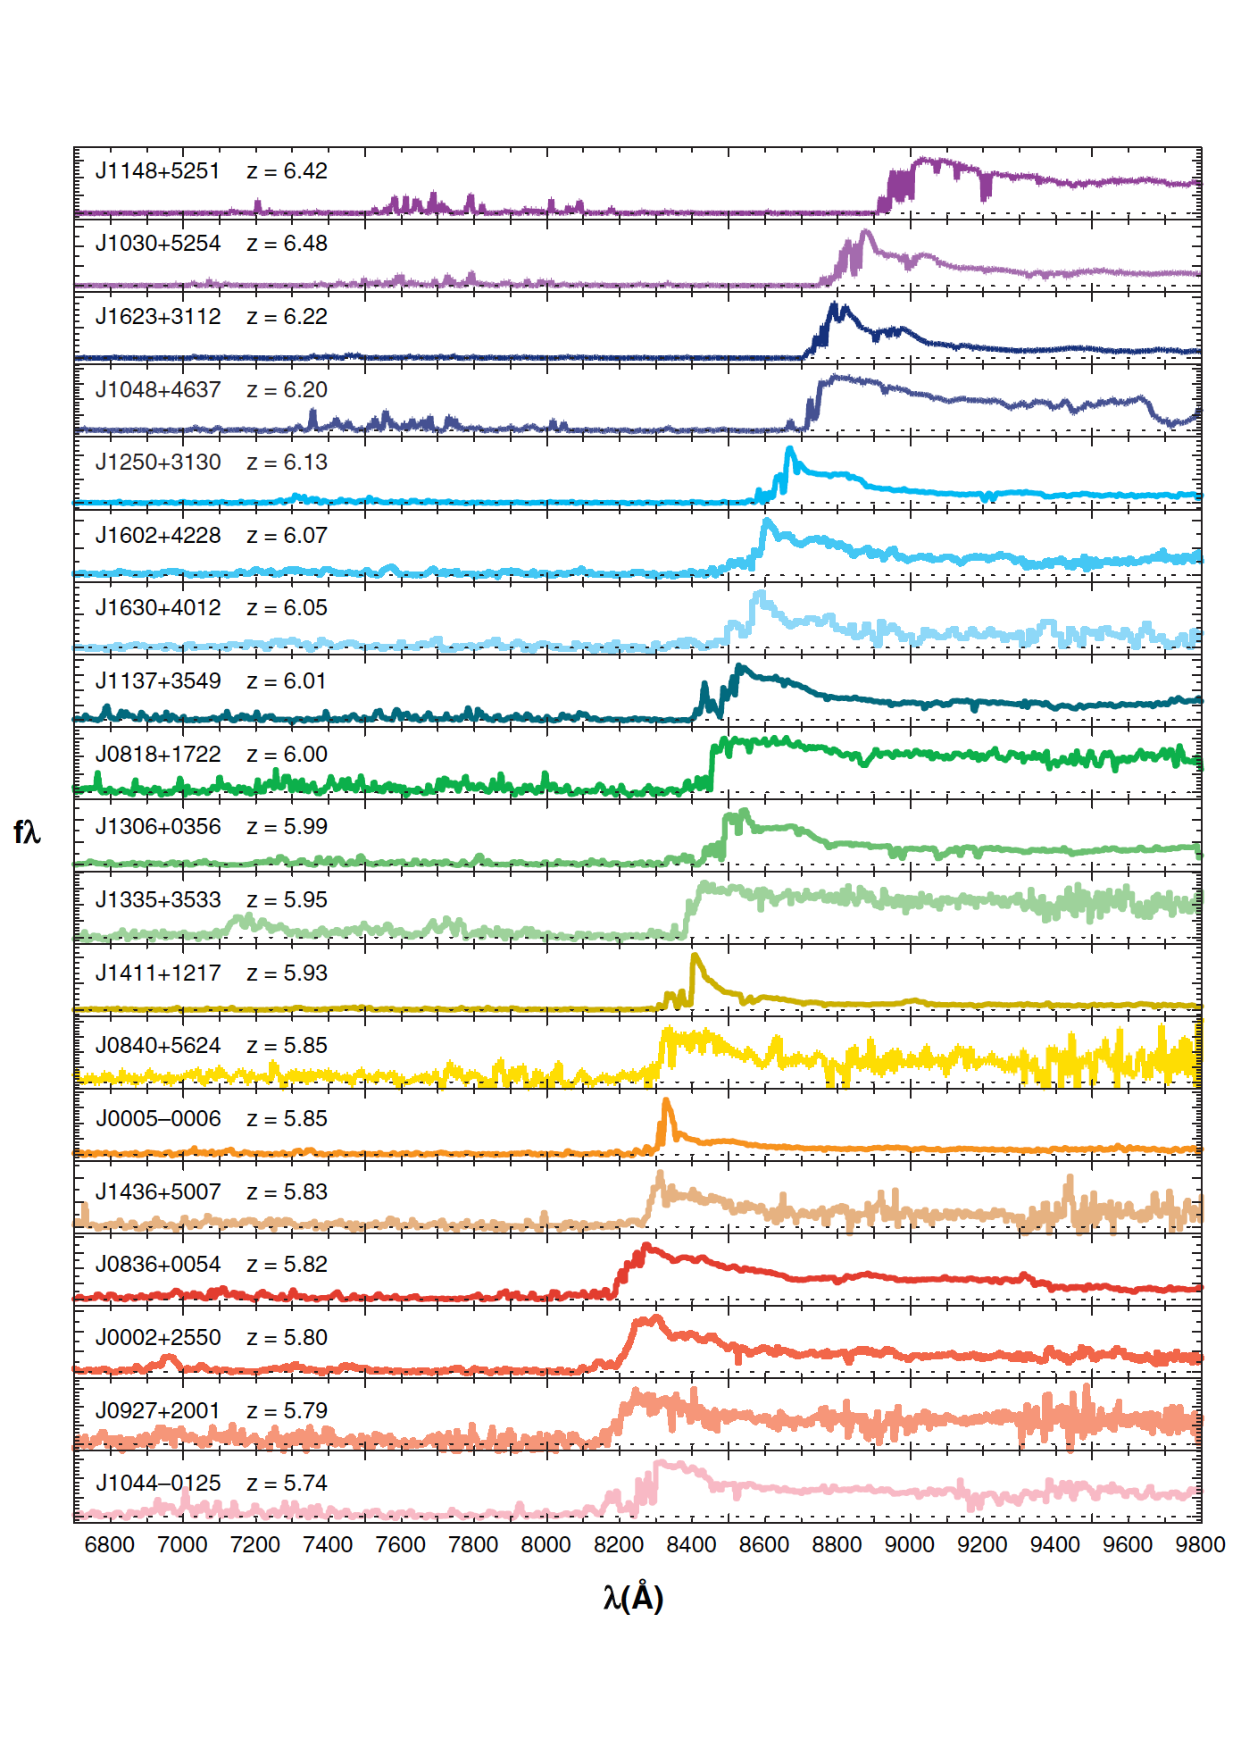
\includegraphics[width=.95\linewidth]{img/01/quasar_spectre.pdf} 
        \caption[Spectre de quasars]{Spectre de quasars à différents redshift présentant un tunnel Gunn Peterson.
		Image extraite de \cite{fan_constraining_2006}.}
 		\label{fig:spectre_quasar}
\end{figure}

\subsubsection{Épaisseur optique}

A partir des spectres obtenu il est possible de mesurer l’épaisseur optique traversée par les photons Lyman alpha à l'aide de la formule suivante:
\begin{equation}
\tau_{GP} = \frac{\pi e^2}{m_e c} f_\alpha \lambda_\alpha H^{-1}(z) n_{HI},
\end{equation}
où $f_\alpha$ est la force d'oscillateur de la transition Lyman alpha, $\lambda_\alpha = 1216 \AA$, $H(z)$ est la constante de Hubble, $n_{HI}$ la densité d'hydrogène neutre.

En appliquant cette formule aux différents spectres observés (figure \ref{fig:spectre_quasar}), \cite{fan_constraining_2006} ont mesurer la variation d'épaisseur optique en fonction du redshift.
Les résultats sont présentés sur la figure \ref{fig:epaisseur_optique_quasar}.
Il apparaît clairement que l'épaisseur optique augmente avec le redshift.

\begin{figure}
        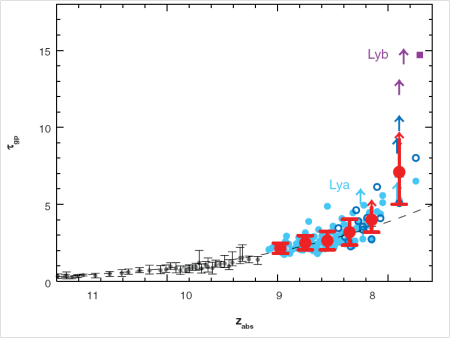
\includegraphics[width=.95\linewidth]{img/01/epaisseur_optique_quasar.png} 
        \caption[Epaisseur optique Lyman alpha]{%https://ism2009.wordpress.com/2009/04/28/on-the-density-of-neutral-hydrogen-in-intergalactic-space/
		Épaisseur optique calculée a partir des spectres de quasar de la Fig\,\ref{fig:spectre_quasar}
        Image extraite de \cite{fan_constraining_2006}.}
 		\label{fig:epaisseur_optique_quasar}
\end{figure}

\subsubsection{Les contraintes sur l'état d'ionisation}

A partir de l'épaisseur optique, il est possible de déterminer la fraction d'hydrogène neutre traversée.
Une compilation des contraintes sur la fraction d'hydrogène neutre a été réalisé par \cite{2015ApJ...811..140B} et est présenté sur la figure \ref{fig:compile_constrains}.
On y observe un brusque changement à redshift $z\approx6$.
Cette chute dans la fraction de neutre représente la fin de la période de réionisation.

\begin{figure}
        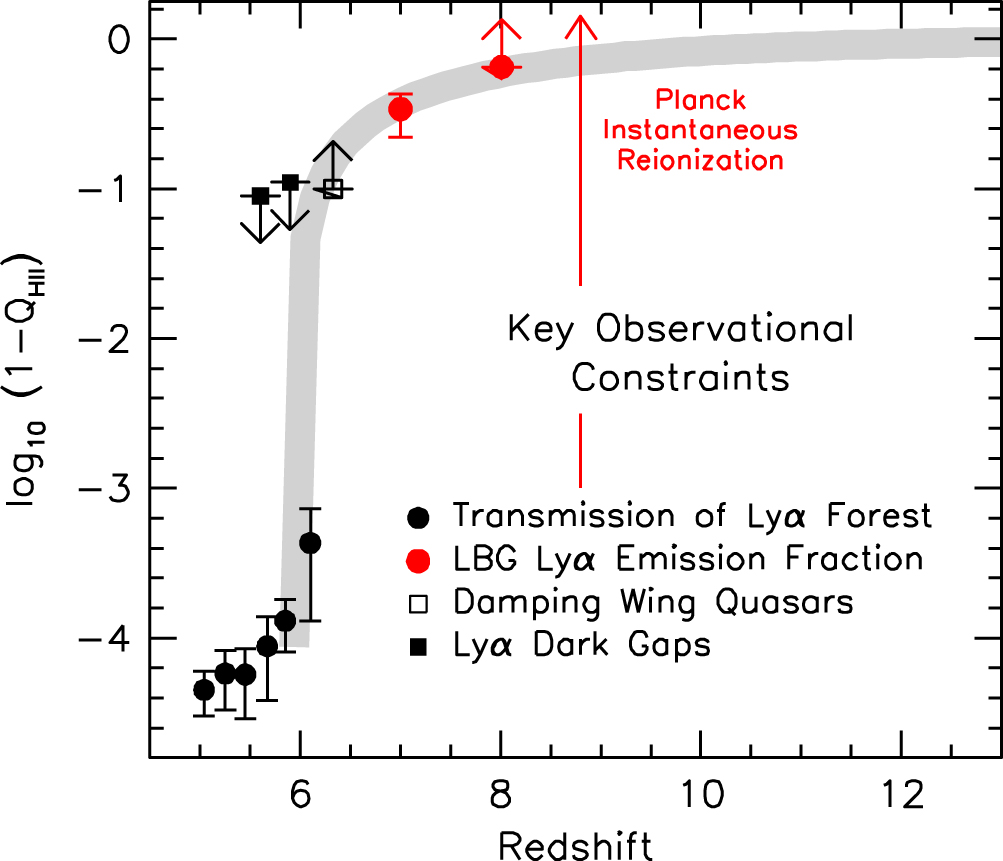
\includegraphics[width=.95\linewidth]{img/01/xionconstrains.jpg} 
        \caption[Fraction de neutre]{Fraction de neutre en fonction du redshift a partir d'observation lymann alpha.
        Compilation par \cite{2015ApJ...811..140B}}
 		\label{fig:compile_constrains}
\end{figure}


\subsection{CMB et épaisseur optique Thomson}

Une observation de la réionisation se trouve également dans les photons CMB, car la réionisation constitue un avant plan qui les a influencé. 
Les photons émis lors de la recombinaisons ont été diffusé, par le grand nombre d'électron libérer pendant la réionisation.
Cette succession de diffusions Thomson, se traduit par une épaisseur optique qui prend la forme : 

\begin{equation}
\tau_z = c \sigma_t \int_z^0 n_e (z) \frac{dt}{dz} dz,
\end{equation}
avec $\sigma_t$ la section efficace Thomson et $n_e (z)$ la densité d'électron libre.

L'épaisseur optique Thomson cesse d'augmenter à partir d'un certain redshift du à l’absence d'électrons libres permettant les diffusions.
Une représentation de cette contrainte, observée par le satellite Planck se trouve sur la figure \ref{fig:epaisseur_optique_thomson}.
Différent modèles réionisation y sont également présentés.
En utilisant un modèle de réionisation instantané, \cite{planck_collaboration_planck_2016} estime le redshift de réionisation à $z_r = 8.8 ^{+1.3}_{-1.2}$.

\begin{figure}
        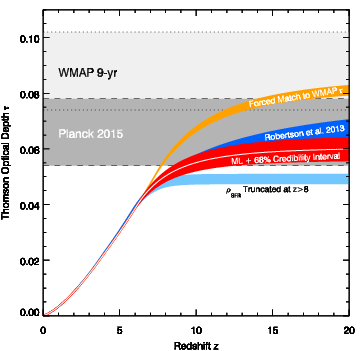
\includegraphics[width=.9\linewidth]{img/01/epaisseur_optique_thomson.png} 
        \caption[Epaisseur optique Thomson]{%https://inspirehep.net/record/1343310/plots
		Contrainte sur l'épaisseur optique Thomson.
        Image extraite de \cite{2015ApJ...802L..19R}
 		\label{fig:epaisseur_optique_thomson} }
\end{figure}

%\subsection{ligne 21 cm}
%
%Une raie a 21 cm est émisse par les nuages d'hydrogène neutre.
%Lorsque que le spin de l'électron et du proton sont opposée, le niveau d'énergie de l'atome est légèrement supérieur au cas ou les spins sont alignés.
%Ces deux niveaux ont des énergies très proches et la transition est dite hyperfine.


%Lors du changement de spin d'un électron 
%
%\subsection{polarisation du CMB)}
%
%\subsection{fonction de luminosité UV}

%\section{Les futures observations}
%\subsection{SKA}
%\subsection{LOFAR}

\section{Quelques questions en suspend}

%quand est ce arrivé?
%quelles sont les sources? -> débat galaxies vs quasars

%En utilisant la halo mass function presenté en TODO REF, 

La provenance des photons qui ont réionisé l'Univers est toujours indéterminée.
En étudiant la répartition du nombre de galaxies en fonction de leurs masses, on observe que les galaxies les moins massives sont nombreuse et que les galaxies les plus massives sont rare.
Or, plus une galaxie est massive, plus celle ci va créer des étoiles, et donc emmètres des photons.
La balance entre les nombreuses galaxies peu lumineuses, et les rare galaxies extrêmement lumineuse reste à déterminer.

De plus, les quasars, objet extrêmement lumineux, situé dans les galaxies les plus massives, augmente encore le budget de photon.
Les quasars ont contribué à réioniser l'Univers mais dans quelles proportion?
Il faut un certain temps pour mettre en place les conditions propices à l'apparition d'un quasar, est ce que ce temps a été suffisant avant z=6, pour en former suffisamment ?
Certain travaux soutiennent que c'est le cas (eg \cite{chardin_large-scale_2017}) cependant seul le rayonnement provenant des galaxies a été considérer lors de cette thèse.

Si ce sont les galaxies qui ont réionisé l'Univers, quelle est le ratio entre la quantité de rayonnement produite et la quantité de rayonnement capable d'atteindre l'\ac{IGM}?
La fraction d'échappement ($f_{esc}$) permet de faire le lien entre les observations et la physique réellement en place au sein des galaxies.
Elles dépend de nombreux paramètres comme la formation stellaire ou les propriétés du milieu.
Comment évolue t-elle en fonction de la masse des galaxies? 

%La figure \ref{fig:gal_AGN} présente le budget de photon plausible pour les galaxies ou les quasars.
%\begin{figure}
%        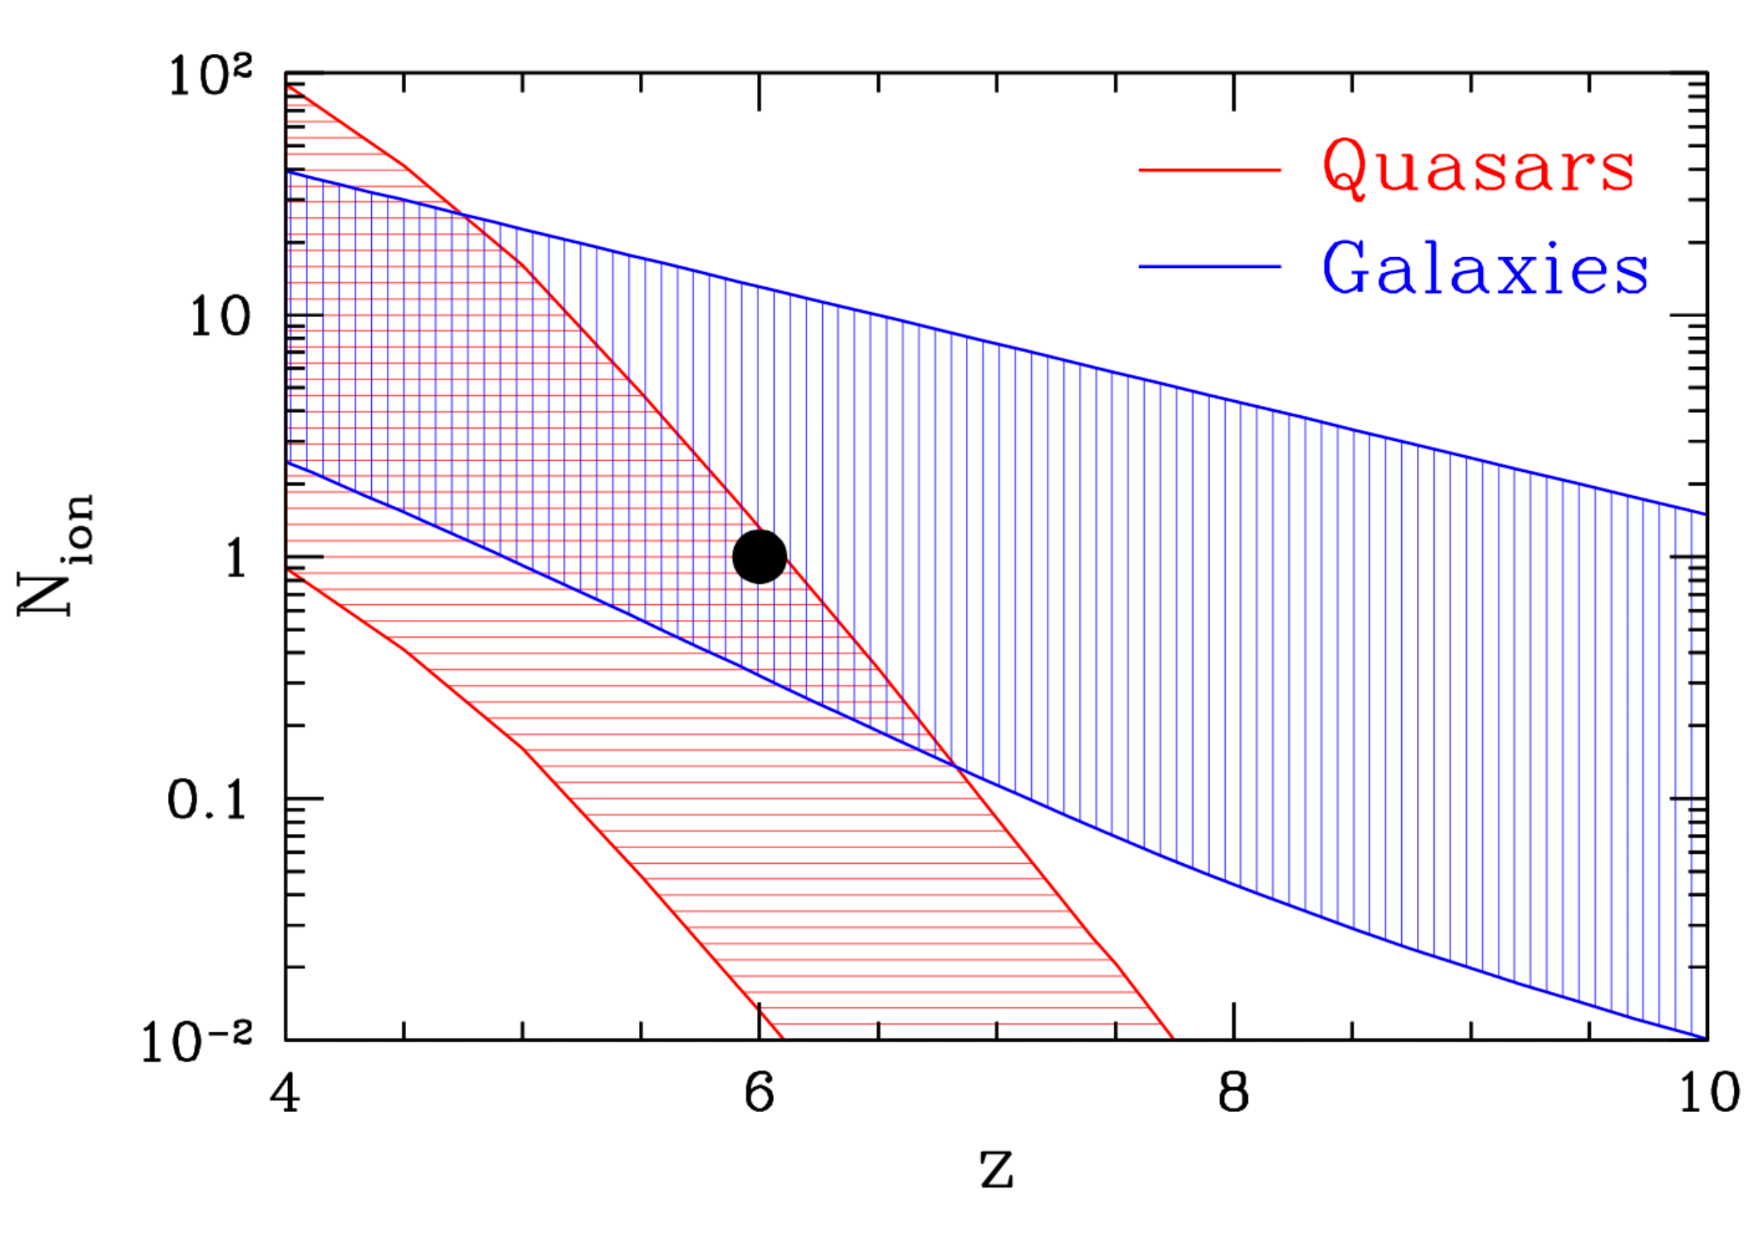
\includegraphics[width=.9\linewidth]{img/01/gal_AGN.pdf} 
%        \caption{Budget de photons provenant des galaxies et des quasars durant la reionization selon \cite{trac_computer_2011}.
% 		\label{fig:gal_AGN} }
%\end{figure}

%outlier dans l'épaisseur optique des quasars
%Le groupe local ?


%\ctparttext{\begin{flushright}{\slshape    
%	Premature optimisation is the root of all evil.} \\ \medskip 
%	-- Donald Knuth
%\end{flushright}
%}
\cleardoublepage
\ctparttext{Cette partie est liée a la publication présentée en annexe\,\ref{pap:EMMA}.\medskip

\emph{"EMMA: an adaptive mesh refinement cosmological simulation code with radiative transfert"}\medskip

Dominique Aubert, Nicolas Deparis et Pierre Ocvirk
2015 MNRAS
}
\part{Methodes numeriques}
\chapter{Introduction a EMMA}\label{ch:introduction}
Les échelles de temps sont radicalement opposées entre la cosmologie qui considère les temps les plus long de l'univers et les progrès informatiques qui vont a une vitesse exponentielle (cf loi de \cite{moore1965cramming}). %\cite{THOMPSON200620}
Les simulations numérique sont des produits possédant une valeur se dépréciant extrêmement rapidement, il faut les considérer comme éphémère.

Nous avons vu dans la partie précédente qu'elles étaient les principales physiques à l’œuvre durant l'époque de réionisation.
L'objectif de cette partie est d'expliquer comment ces physiques sont modélisées et implémenté informatiquement.

%Comment modéliser la reionization?

\section{Aperçu des différents types de code}

Un code de simulation cosmologique a pour vocation principale de suivre l'évolution de différents "fluides", comme la matière noire, la gaz, les étoiles, la radiation ou le champ magnétique.
Ces fluides sont de nature différentes et il n'y a pas de méthode unique permettant de suivre de manière optimale ces différentes physique.
On distinguera principalement deux catégories de fluides: les collisionnels et les non-collisionnels.

\paragraph{La physique non-collisionnelle} concerne les phénomènes qui n'interagissent pas par collision.
Il s'agit principalement la matière noire et les étoiles. 

\paragraph{La physique collisionnelle} concerne principalement le gaz.

Il existe conceptuellement deux principales façons de suivre un fluide dans l'espace.
Ces deux approches sont dites \emph{Eulérienne} ou \emph{Lagrangienne}.

\paragraph{Représentation Lagrangienne : } 
consiste a se placer au point de vue du fluide.
On considère un élément de fluide de masse fixe pouvant se déplacer et/ou se dilater dans l'espace.
On associera généralement les codes utilisant ce type de représentation avec une gestion de la physique sous forme de \emph{particules}.

\paragraph{Représentation Eulérienne : } 
consiste a se placer au point de vue de l'espace.
On considère un élément d'espace et le bilan de matière entrant et sortant de chacune de ses interfaces.
On associera généralement les codes utilisant ce type de représentation avec une gestion de la physique sous forme de \emph{grille}.

En lien direct avec ces deux familles de représentation physique, il existe deux principales famille de codes cosmologique : les codes \ac{SPH} et les codes \ac{AMR}.

\paragraph{Smooth Particle Hydrodynamic (SPH) : } représente le gaz sous forme de particule de masse constante mais de taille variable.
%Notion d'arbre -> KDtree

\paragraph{Code sur grille} : représente l'espace sous forme de cellules organisées sur une grille. 
Si la grille est de résolution variable on parlera de grille AMR (Adaptive Mesh Reffinement) 


%Notion d'arbre -> arbre AMR
%La représentation Lagrangienne la plus populaire (dans le domaine des simulations cosmologiques) est sans doute le \emph{Smouth Particle Hydrodynamics (SPH) }
%Les volumes cosmologiques étant généralement cubique, les éléments de grille le sont généralement aussi.
%historique
%avantage inconvénient AMR vs SPH
%introduction de la grille et de la méthode AMR


Un même code peux utiliser conjointement plusieurs des concepts qui viennent d'etre exposés.
Par exemple EMMA utilise une représentation Lagrangienne pour simuler la physique non collisionnelle de la matière noire et une représentation Eulérienne pour simuler le gaz et la radiation.

\section{Gestion de la grille}
\label{sec_gestion_grille}
%(nécessaire d'être positionné ici car la structure en arbre conditionne plusieur choix par la suite)

La grille adaptative étant commune a tout les solveurs.
Nous allons la dévelloper avant de détailler la gestion de la physique. 

Avant d'aborder le concept de grille adaptative faisons un leger détour par l'exemple d'une grille fixe et régulière.
Dans le cas des simulations sur grille fixe, les données sont réparties en mémoire de façon ordonnée.
Dans un espace en 3D, on accédera à une cellule contenant le point de coordonnées normées $(x,y,z)$ sur une grille de $N_x*N_y*N_z$ cellules, a l'aide de son identifiant Id dans le tableau en mémoire.

\begin{equation}
Id = i + j*N_x + k * N_x*N_y
\end{equation}
avec :
\begin{equation}
\begin{cases}
i=\lfloor x \rfloor *N_x \\
j=\lfloor y \rfloor*N_y \\
j=\lfloor z \rfloor*N_z \\
\end{cases}
\end{equation}
ou $\lfloor a \rfloor$ représente la partie entière de $a$.

Les choses sont plus complexes dans le cas d'une grille adaptative (Fig \ref{fig:AMR}).

\begin{figure}[bth]
        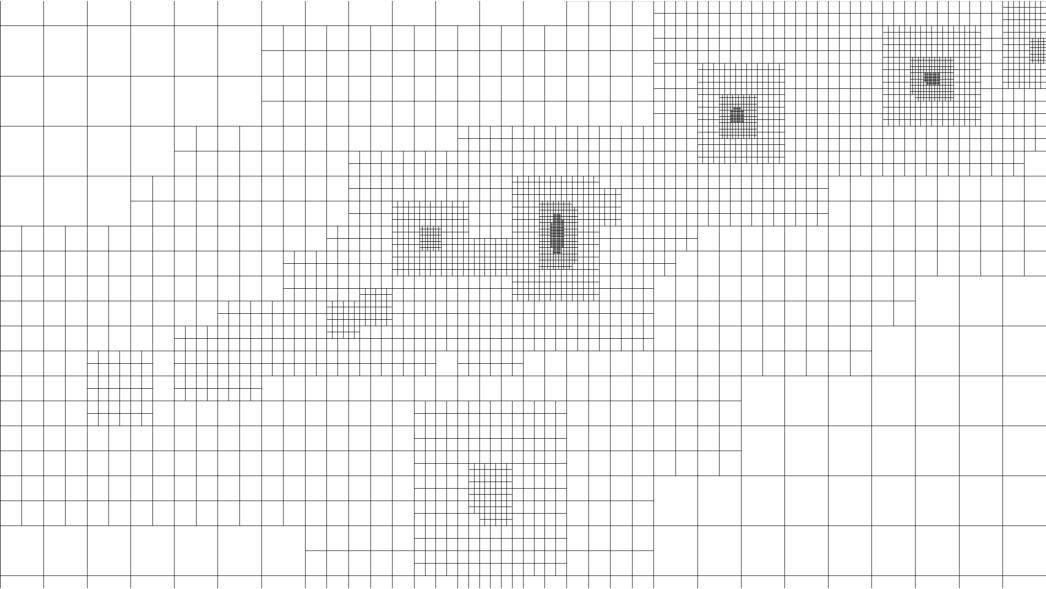
\includegraphics[width=.95\linewidth]{img/02/AMR.pdf} 
        \caption{Exemple de grille AMR. 
        La  résolution de la grille est augmentée dans les régions d'intérets.
}
 		\label{fig:AMR}
\end{figure}


\subsubsection{Octree}

Il existe deux grand groupe de maille adaptative.
Le premier groupe utilise des grilles fixes imbriquées %TODO ref

Le second est le groupe qu'utilise EMMA : fully threated tree description \citep{khokhlov_fully_1998-1}.
La base de cette représentation est de considérer que chaque cellule est associée a une grille 2x2x2 que l'on nommera un OCT (cf:\ref{lst:oct}), car décomposé en 8 sous parties qui sont elles même des cellules (cf:\ref{lst:cell}).
Et récursivement, chacune de ses sous parties peut a leurs tour être divisé ou non.
il en résultera un arbre nommé Octree.

\begin{figure}[bth]
        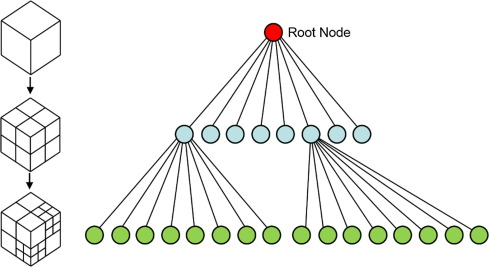
\includegraphics[width=.95\linewidth]{img/02/octree.jpg} 
        \caption{Représentation d'une grille AMR a gauche, et de son octree associé a droite. 
        Image extraite de \cite{SU201659}
}
 		\label{fig:octree}
\end{figure}

\subsubsection{Liste chainée}

Comme la grille est amenées a évoluer, il n'y a plus une position unique en mémoire associé à une position dans l'espace.
La grille est composée de cellules ordonnées sous forme de liste chainées.
Pour créer un lien entre elle, il est nécessaire de stocker l'information de voisinage.
Pour localiser un oct dans l'espace, on a besoin de stocker 2*D pointeurs vers les cellules voisine.
Un oct est également composé de d'un tableau de huit pointeurs vers ses huit cellules filles,  ainsi que d'un pointeur vers sa cellule mère.
On associera ensuite au cellules la partie physique (densité, pression, température, etc...).
Ainsi chaque cellule peut, sous certaine condition, etre subdivisée en un OCT pour augmenter la résolution localement.


On associera également les octs entre eux a l'aide d'une liste chainée. 
Il est nécessaire d'ajouter deux pointeurs a l'objet OCT : un vers l'oct précédent en mémoire et un vers l'oct suivant.

\begin{lstlisting}[float=bth,language=C,frame=tb,caption={les structures cellule de EMMA},label=lst:cell]
struct CELL{
  int id;            // permet de determiner la position de la cellule dans l'oct
  struct OCT *parent // l'oct pere de la cellule
  struct OCT *child; // si child est different de NULL alors la cellule est raffinee et child point vers l'oct enfant
  struct PHYSIC *data; // pointeur vers la partie physique
};
\end{lstlisting}

\begin{lstlisting}[float=bth,language=C,frame=tb,caption={les structures OCT  de EMMA},label=lst:oct]
struct OCT{
  struct CELL cell[8]; // les 8 cellules de l'oct
  struct CELL *nei[6]; // pointeurs sur les cellule voisines
  struct CELL *parent; // cellule mere
  struct OCT *next;    // oct suivant dans la liste chainee
  struct OCT *prev;    // oct precedent dans la liste chainee
  int level;           // niveau de l'oct
};
\end{lstlisting}


Terminologie:
On parlera de :

RACINE pour l'OCT de niveau 0. Il n'a pas de cellule mère et représente l'ensemble de l'espace de la grille.
La génération de conditions périodique (généralement utilisées en cosmologies) se fait de manière naturelle en faisant pointer tout les voisins de l'OCT racine vers lui même.


FEUILLE pour les cellules qui ne sont pas raffinées. 



\subsubsection{Gestion du raffinement}
\label{sec:raffinement}
%différentes condition de raffinement.\\
%sur la matière noire\\
%semi Lagrangienne\\
%sur le gradient d'ionization\\
%sur le gradient de densité (shock)\\

Il est possible de définir arbitrairement une condition de raffinement en fonction de la physique que l'on cherche a étudier.
Par exemple, dans des tests unitaires de type sphère de Stömgren ou explosion de Sedov, on marquera les cellules qui sont soumises a un gradient d'ionisation ou de densité supérieur a un certain seuil.
%TODO ajouter les ref des sections pour sedov et stromgren
Dans le cas de simulations cosmologique, on utilisera généralement une condition dite semi-Lagrangienne.
C'est a dire qu'une cellule sera marquée comme "a raffinée" si la masse de matière noire (ou de gaz) qu'elle contient est supérieur a huit fois la masse de matière noire (ou de gaz) moyenne d'une cellule de ce niveau.



En pratique, le raffinement se fera en trois temps:

\begin{itemize}
\item Dans un premier temps le code va passer en revue toutes les cellules d'un niveau, et les marquer comme "a raffiner" si une première condition physique est respectée.

\item Une fois tout le niveau passé en revue, le code va ensuite faire une série de $N_{buffer}$ passages sur tout le niveau en marquant à chaque fois les cellules voisine des cellules précédemment marquées.
Cette série de passage a pour but d’élargir la zone de raffinement et ainsi permettre une transition douce entre les niveaux.
Cette zone de $N_{buffer}$ cellules autour des zones soumises à la condition physique de raffinement sera appelée le "buffer de raffinement".

\item Une fois les cellules respectant ces deux conditions marquées, le raffinement est effectué.
\end{itemize}

En pratique le raffinement d'une cellule se fera en lui associant un OCT.
*child pointera alors vers le dernier OCT libre de la liste chaînée.

%le deraffinement
On remarquera que la condition de raffinement ne prends pas en compte le fait qu'une cellule soit déjà raffinée ou non.
Si une cellule est raffinée, mais qu'elle n'est pas marquée comme "a raffinée" elle sera donc dé-raffinée.

\subsubsection{Opérateurs de changement de grilles} \label{Opérateurs de changement de grilles}

Les opérations de raffinement/dé-raffinement font intervenir des opérateurs de changement de grille.
Le changement de résolution peut avoir lieu dans les deux sens :

\begin{itemize}
\item La \emph{restriction} consiste à dégrader la grille en résolution. La restriction la plus directe consiste à moyenner les cellules à dégrader. Par exemple, sur une grille à deux dimensions, pour diviser la résolution par deux, quatre cellules de la grille de départ devront être moyennées pour obtenir une nouvelle cellule de la grille à base résolution.

\item La \emph{prolongation} consiste à augmenter la résolution d'une grille, la prolongation la plus directe consiste à injecter les valeurs de l'ancienne grille dans un certain nombre de cellules de la nouvelle grille. (fig \ref{Opérateurs de changement de grille})
\end{itemize}

\begin{figure}[htbp]
\begin{center}
\subfloat[Restriction]{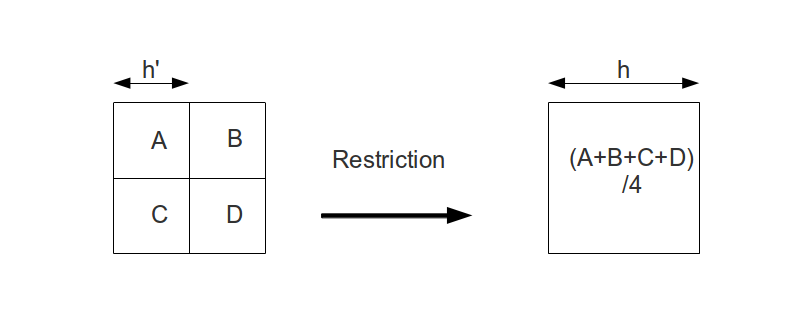
\includegraphics[width=.45\linewidth]{img/02/Restriction.png}}
\subfloat[Prolongation]{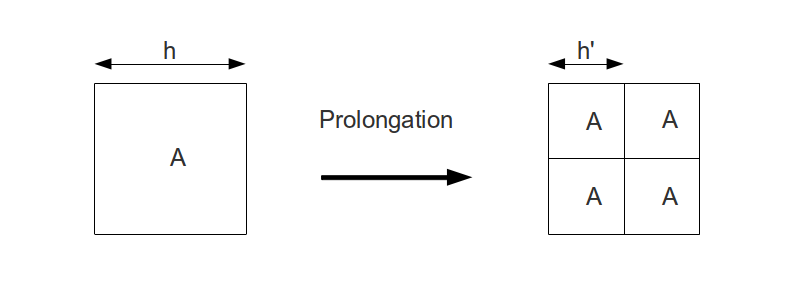
\includegraphics[width=.45\linewidth]{img/02/Prolongation.png}}\\
\subfloat[Niveau L  ]{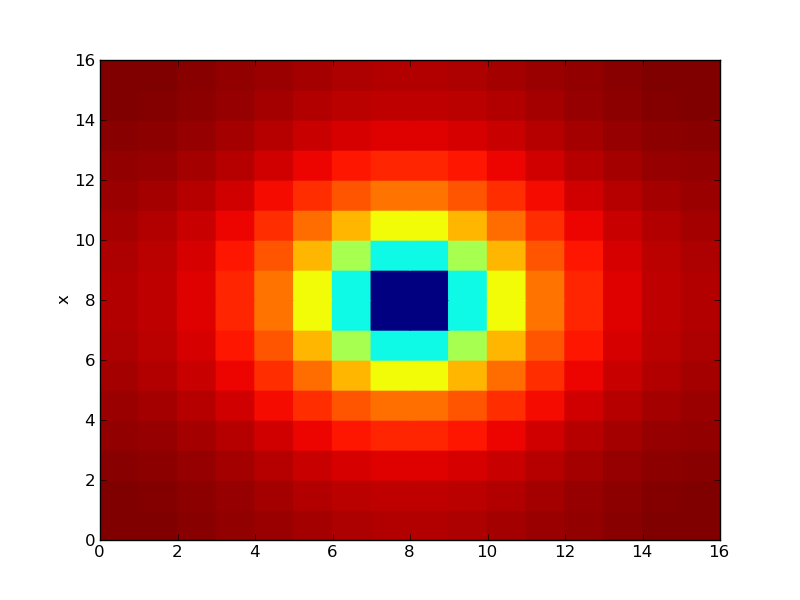
\includegraphics[width=.45\linewidth]{img/02/0090.png} \label{Opérateurs de changement de grille d}}
\subfloat[Niveau L+1]{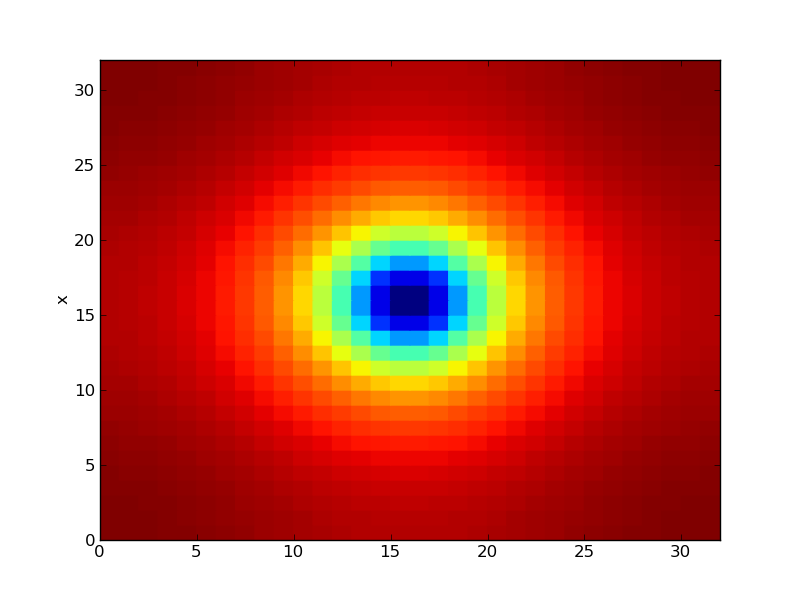
\includegraphics[width=.45\linewidth]{img/02/0088.png} \label{Opérateurs de changement de grille c}}
\caption{Opérateurs de changement de grille. 
Ils permettent de changer la résolution de la grille. Un exemple de restriction consiste à moyenner une valeur de plusieurs cellules, la prolongation associée consiste en une injection directe d'une valeur dans plusieurs cellules.}
\label{Opérateurs de changement de grille}
\end{center}
\end{figure}

La prolongation et la restriction sont des opérateurs aisément parallélisables. Chaque cellule (ou paquet de huit cellules) est indépendante des autres et il est possible de ne changer la résolution que d'une partie de la grille sans en affecter le reste.\\

Il existe principalement deux conditions sur les opérateurs de changement de grille. 
La première impose une certaine réciprocité entre eux, les opérateurs doivent être adjoints: il est nécessaire qu'après une prolongation, suivie d'une restriction la grille d'arrivée soit la même que la grille de départ. 
L'inverse n'est pas nécessairement vrai: après une restriction, de l'information est perdue et aucune prolongation ne pourra la recomposer.
La seconde condition concerne la precision des opérateurs, il est nécessaire que la somme des ordres des opérations soit supérieure à l'ordre de l'équation à résoudre. 
Ici, la restriction est d'ordre trois, la prolongation d'ordre un et le Laplacien d'ordre deux, cette condition est vérifiée.


\subsection{Recherche de voisin}
Nous verrons par la suite que l'état d'une cellule dépend des états des cellules qui l'entoure.
La recherche de voisins sera donc une étape importante dans la gestion de la grille.

La recherche de voisin se fera suivant ces étapes:

\begin{itemize}
\item en fonction de l'ID de la cellule, déterminer si la voisine est dans le même OCT parent.


\item
\begin{itemize}
\item Si c'est le cas, accéder a l'oct parent et a l'aide de l'indice du tableau de cellule, retrouver le voisin en question.
\item Si ce n'est pas le cas, accéder a la cellule mère de l'oct père et rechercher l'oct voisin
\end{itemize}

\end{itemize}


Nous avons vu dans la partie d'introduction a la physique de la reionisation que l'énergie noire représente la majore partie du contenu de l'univers.
Nous allons voir dans cette partie comme cette composante est simulée.

Bien que nous sachions absolument pas ce que peux être physiquement l'énergie noire, nous en observons les effets : l'Univers est en expansion accélérée.
Le solveur gérant l'énergie noire n'est pas a proprement parler un solveur numérique, mais plutôt d'un système d'unité. % servant a normaliser la physique.
Il consiste a normaliser les grandeurs par une variable fonction du facteur d'expansion.

% mais est la plus simple a simuler.
%Lien direct avec le facteur d'expansion (mettre ref section).

L'intégration de la cosmologie, régissant le lien en le temps et le facteur d'expansion sera réalisé une fois au moment de l'initialisation du code. %TODO ref
Il en résultera une table, conservée en mémoire pendant toute l'exécution.
Le facteur d'expansion sera alors interpoler dans cette table ne fonction de l'avancement de la simulation (cf partie calcul du pas de temps) %TODO ref

\subsection{Gestion de l'expansion}
Il existe deux possibilités pour modéliser l'expansion de l'univers a l'aide d'une grille.
La première consiste a considérer un élément de volume $dx$ de taille fixe, et au fur et a mesure que l'univers grandis, a y ajouter des éléments.
Le problème et que le coût numérique de la simulation croit, entre autre, avec le nombre d'éléments que l'on considère.
La seconde possibilité est de faire varier la taille des éléments de calcul avec le facteur d'expansion.
On appellera les longueurs ainsi exprimées des longueurs comobile.

\begin{equation}
r=a r'
\end{equation}

ou $r$ représente une longueur en unités physique et $r'$ en unités comobile.

Ainsi un cube de 10 Mpc physique de coté, pris aujourd'hui, aura une taille de 10 Mpc comobile (cMpc) aujourd'hui, mais aussi a redshift z=9 ou sa taille physique ne sera plus que de de 1Mpc physique.

De plus, il est généralement pratique de normaliser les grandeurs que l'on considère. 

\begin{equation}
r'=\tilde{r}r*
\end{equation}
ou $\tilde{r}$ est la longueur normalisée et $r*$ le facteur de normalisation.

La généralisation de ce principe a d'autre unités que la longueur est appeler système d'unités supercomobiles.
\citep{martel_convenient_1998}

\begin{table}[htbp]
\begin{center}
\begin{tabular}{r l} \hline 
Longueur: & $\tilde{r}=\frac{r}{ar_*}$ \\ \hline 
Densité de matière: & $\tilde{\rho}=\frac{\rho a^3}{\rho_*}$ \\ \hline 
Vitesse: & $ \tilde{v}=\frac{av}{v_*}$ \\ \hline 
Pas de temps: & $\tilde{dt}=\frac{dt}{a^2t_*}$\\ \hline 
Densité d’énergie potentielle: & $\tilde{\Phi}=\frac{a^2 \Phi}{\Phi_*}$\\ \hline 
Pression: & $\tilde{p}=\frac{a^5 p}{p_*}$\\ \hline 
Densité d’énergie cinétique: & $\tilde{\epsilon}=\frac{a^2 \epsilon}{\epsilon_*}$\\ \hline 
Densité D’éléments: & $\tilde{N}=a^3 N r_*^3$\\ \hline 
Flux: & $\tilde{F}=a^4 r_*^2 t_* F$\\ \hline 
\end{tabular} 
\end{center}
\caption{Passage du système d'unités physique vers le système d'unité supercomobile} 
\end{table}

\begin{table}[htbp]
\begin{center}
\begin{tabular}{r l} \hline 
Longueur  & $r_*=L$\\ \hline 
Densité & $\rho_* = \bar{\rho} = \frac{3H_0^2 \Omega_m}{8\pi G}$\\ \hline 
Temps & $t_* = \frac{2}{H_0 \sqrt{\Omega_m}}$\\ \hline 
Vitesse & $v_* = \frac{r_*}{t_*}$\\ \hline 
Potentiel & $\Phi_* = \frac{r_*^2}{t_*^2} = v_*^2$\\ \hline 
Pression & $p_* = \frac{\rho_* r_*^2}{t_*^2} = \rho_* v_*^2$\\ \hline 
Énergie & $\epsilon_* = \frac{p_*}{\rho_*} = v_*^2$\\ \hline 
\end{tabular} 
\end{center}

\caption{Facteurs de normalisation des différents grandeurs physique} 
\end{table}




\subsection{Gestion du pas de temps}


\begin{equation}
\frac{\delta a (\Delta t) } {a} < \epsilon
\end{equation}


\chapter{Les principaux solveurs physique}

Nous allons voir dans cette partie que plus une physique représente une part importante du contenu de l'Univers plus elle est simple et rapide a simuler.
Nous nous intéresserons a quatre solveurs distinct:
\begin{itemize}
\item d'énergie noire
\item de matière noire
\item du gaz
\item de la radiation
\end{itemize}
Et ce, dans un ordre décroissant d'importance, relativement a la quantité d'énergie totale.


%%%%%%%%%%%%%%%%%%%%%%%%%%%%%%%%%%%%%%%%%%%%%%%%%%%%%%%%%%%%%%%%%%%%%%%%%%%%%%%%%%%%%%%%%%%%%%%%%%%%%%%%%%%%%%%%%%%%%%%%%%%%%%%%%%%%%%%%%%%%%%%%



%%%%%%%%%%%%%%%%%%%%%%%%%%%%%%%%%%%%%%%%%%%%%%%%%%%%%%%%%%%%%%%%%%%%%%%%%%%%%%%%%%%%%%%%%%%%%%%%%%%%%%%%%%%%%%%%%%%%%%%%%%%%%%%%%%%%%%%%%%%%%%%%
\section{Matière noire}
\label{sec:solverDM}
La matière noire, dispose de propriétés de fluide non collisionelle, et se prête particulièrement bien a la représentation Lagrangienne, et donc a une simulation sous forme de particule.
Pour la simuler, on utilisera le principe des code Ncorp., c'est a dire qu'on utilisera un champs de particules massive interagissante par gravitation.
Ill existe différentes techniques pour suivre l'évolution d'un tel système.
Toutes sont basé sur le meme principe.
Les particules sont placée suivant une certaine condition initiale.
Et on cherche a connaitre la force gravitationnelle a laquelle chaque particule est soumise, dans le but de calculer son déplacement


\subsection{Génération des conditions initiales}

Nous avons vu %TODO ref
que le CMB nous donne de l'information sur l'état de la distribution de matière dans l'univers tres tot dans son histoire (il est possible de determiner le spectre de puissance des fluctuation de densité de l'univers primitif).
Le principe de la génération des condition iniales est d'utiliser ce spectre de puissance pour générer des surdensité repréentant statistiqument ces fluctuations.

Pour se faire on va générer une grille regulière sur laquelle on placera une particule au centre de chaque cellule.
Dans ce cas la densité est homogène.
On va alors perturber la position des particules de manière a respecter les fluctuations statistique observées dans le CMB.

Pour ce faire, il faut générer un bruit aléatoire Gaussien.
Tout les générateurs de condition initiales que j'ai pus rencontrer utilise une SEED aléatoire, dans le but de générer ce bruit aléatoire.
On convoluera ensuite ce bruit avec le spectre de puissance que l'on cherche a reproduire.

Et on appliquera les déplacement obtenus au particules.

Cette approximation n'est valable que dans le cas des petites perturbations, tant que l'on reste dans le régime linéaire.
Cette approximation du regime linéraire s'appelle l’approximation de Zeldovitch %TODO ref
\cite{2014MNRAS.439.3630W}


Plus l'on cherche a simuler des petites échelles, plus l'on sort vite du domaine de précision accéptable.
C'est pourquoi il est necessaire d'avoir recourt au simulations numériques.

Nous voyons ici que le spectre est limité des deux cotés.
D'un coté l'information des grandes échelles est tronquée par la taille de la boite considéré.
Il n'est pas possible d'avoir de l’information sur des longueurs d'onde du spectre plus grande que cette taille limite.
De l'autre coté, les petites échelles sont tronquées par la limite de résolution.
Le spectre est troqué au niveau de la longueur d'onde correspondant a la résolution de la grille.

Au passage cette perte d'information sur les hautes fréquences peux être problématique dans le cas ou la résolution est adaptative.
Dans le cas de l'AMR par exemple il peux paraître difficile d'autoriser un nombre élevé de niveau de raffinement puisque les niveaux nouvellement créer ne disposerons pas de l'information des conditions initiales.

En pratique j'ai principalement utilisé MUSIC et GRAPHIC %TODO ref.


%méthode
%gaussian random noise
%théorie des perturbation linéaire
%lien avec le spectre de puissance
%MUSIC et GRAPHIC
%limite la résolution min et max (min en masse et max en espace)


%une simulation est limité par sa taille et sa résolution -> ceci définit la plage d'échelle que l'on peut simuler
%
%principes de bases ennoncé dans Pen (1997) and Bertschinger (2001).
%
%    discrétisation de l'espace
%    placement des particules sur la grille
%    génération d'un bruit blanc
%    convolution avec un spectre de puissance connu (celui du CMB)

%
%\subsection{Théorie des perturbation linéaire}
%
%approximation de zeldovich
%perte de linéarité a un certain moment -> nécessité des simulation numériques





\subsection{Solveur de gravité}

A partir des condition initiales nouvellement générées, il faut ensuite suivre dynamiquement l'évolution des particules.

Je vais plus détailler le solveur de gravité que les autres puisque c'est celui sur lequel j'ai le plus travaillé.
%Le sloveur que je connais le mieux.
%Fluide non collisionnel -> particule\\

On cherche a obtenir la position des particules a chaque instant.
Pour cela, il nous faut leurs vitesses.
Pour cela, il nous faut leurs accélération.
Pour cela, il nous faut la force qui leur est appliquée.

Ce système d'équation est appelé le système d'équation de Vlasov-Poisson :

\begin{equation}
\begin{cases}

\frac{d{x}_p}{dt} = { v}_p, \\
\frac{d{ v}_p}{dt} = -\nabla \phi , \\
\Delta \phi= 4\pi G \rho.

\end{cases}
\label{eq:Ncorps}
\end{equation}

Il existe plusieurs méthodes pour résoudre ce système.
Historiquement la première méthode était le méthode :

\paragraph{Particule-Particule : } c'est le méthode la plus directe pour calculer l'évolution d'un fluide non collisionnel. 
Elle consiste, pour chaque particule, a sommer les contribution gravitationnelles de toutes les autres particules.
Ce type de code dispose d'une très bonne précision mais la quantité de calcule évolue en ordre $O(N^2)$, ce qui fait que ce type de code est très coûteux.

\begin{equation}
\vec{F}_i=-\sum_{j\neq i} G \frac{G m_i m_j(\vec{r}_i - \vec{r}_j) }{ |\vec{r}_i - \vec{r}_j |^3}
\end{equation}

Une évolution de cette méthode est la méthode :

\paragraph{Particule-tree : } elle  consiste a regrouper les particules loin de la particule courante en un amas aillant une interaction gravitationnelle commune
% (Barnes & Hut 1986) 
Cette approximation permet de limiter considérablement le nombre de calcul pour les interactions lointaine qui sont de toute façons faibles.


Une autre méthode, celle qui nous intéresse ici consiste a utiliser le potentiel:

%On peux obtenir cette force soit par calcul direct, soit par dérivation du potentiel.

\begin{equation}
\vec{F}=-\Delta \Phi
\end{equation}

Le potentielle sera calculé sur une grille, cette méthode sera nommée :
\paragraph{Particule-Mesh : } on projette les particules sur une grille
ENZO %code, Bryan & Norman 1998
RAMSES

La méthode de projection des particules sur la grille n'est pas unique.
On peut par exemple se contenter d'ajouter la masse de la particule dans la cellule a laquelle elle appartient.
Cela donne un résultat très bruité.
Une méthode d'ordre supérieure est appelé Cloud in cell (CIC)

\paragraph{Cloud in cell : } Le CIC consiste a considérer une étendue spatiale aux particules et a pondérée la masse appliqué au cellule par l'intersection de de son volume et de celui de la cellule.
Fig\,\ref{fig:CIC}.
On associe généralement une taille a la particule similaire a celle des cellule sur laquelle on la projette.
Dans le cas ou L’étendue de la particule intersecte des cellules de différents niveaux on lui associera la taille de la plus grande cellule dans le but de lisser la transition entre les niveaux.


\begin{figure}[bth]
		\centering
        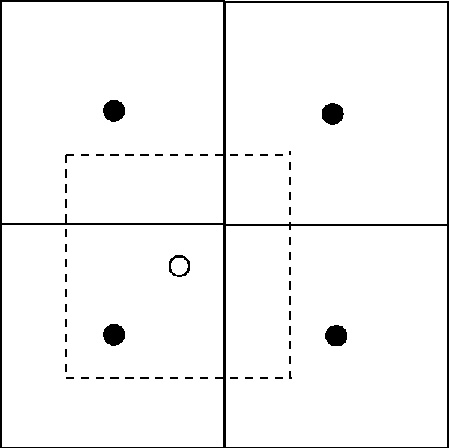
\includegraphics[width=.5\linewidth]{img/02/CIC.jpg} 
        \caption{Représentation en 2D du Cloud In Cell. 
        La masse d'une particule est répartie dans le cellules environnantes en lui associant une étendue spatiale.
        %http://homepage.univie.ac.at/franz.vesely/cp_tut/nol2h/new/c6sm_s4lr.html
}
 		\label{fig:CIC}
\end{figure}

Il existe des méthodes d'ordre supérieur avec des kernel plus complexe que le top-hat du CIC comme par exemple des kernel en triangle ou en gaussienne.
%http://techfinder.stanford.edu/technology_detail.php?ID=30866

Une fois la grille de densité générée nous pouvons calculer le potentiel.

\subsubsection{l'équation de Poisson}
\begin{equation}
\Delta \Phi = 4 \pi G \rho
\end{equation}

qui devient en système d'unité supercomobile:
\begin{equation}
\Delta \Phi = 6 a \delta
\end{equation}
avec le contraste de densité: 
\begin{equation}
\delta = \tilde{\rho} / < \tilde{\rho} > - 1 
\end{equation}

integration de l'equation de Poisson pour obtenir le potentiel
\begin{equation}
\Delta \phi = 4\pi G \rho \longrightarrow \phi = \iint \Delta \phi = \iint 4\pi G \rho
\end{equation}

Pour cela, il existe principalement deux types de méthodes. La première est basée sur les Transformées de Fourier. Cette méthode, très rapide, utilise le fait que dans l'espace de Fourier, une intégrale se résume à une division par un nombre d'onde. Déterminer le champ de potentiel revient à : 
\begin{itemize}
\item Effectuer la transformée de Fourier de la densité
\item Diviser par $k^2$
\item Effectuer la transformée de Fourier inverse
\end{itemize}

\begin{equation}
\rho_{(\vec{x})} \overset{FFT}{\longrightarrow}  \rho_{(\vec{k})} \times \frac{1}{k^2}  \overset{RFFT}{\longrightarrow}  \phi_{(\vec{x})}
\end{equation}

De par la nature des transformées de Fourier, le champ de densité doit être périodique pour que l'implémentation de cette technique ne se révèle pas trop complexe. Ce qui n'est pas un problème en simulation cosmologique, où les conditions de bords sont toujours périodiques mais est plus problématique lors de la simulation de structures isolées, telles les galaxies ou les amas de galaxies. Ensuite, les FFT nécessitent un échantillonnage régulier ce qui implique que cette méthode est incompatible avec les grilles adaptatives. Et dernièrement, le passage dans l'espace des fréquences nécessite des conditions de types plans parallèles lors parallélisation, conditions incompatible avec la gestion de grille utilisé par les code AMR dont \emph{Quartz} fait partie. \\

Un autre type de méthode de résolution possible est une méthode itérative. Elle consiste à faire converger le potentiel à partir d'une condition initiale arbitraire. Ce type de méthode est plus lente que la méthode par FFT mais  permet d'utiliser tout type de conditions de bords, d'être facilement parallélisable et surtout est compatible avec les méthodes basées sur des grilles adaptatives. PAr la suite, c'est donc une méthode itérative et plus précisément une méthode \emph{Multigrille} qui à été développée.\\

Le potentiel est alors dérivé pour obtenir la force ressentie dans chaque cellule. Il est ensuite aisé de calculer l'accélération subie par les particules de chaque cellule, et par intégration temporelle, leurs nouvelles positions et vitesses.

Par analogie à l'équation de la chaleur par exemple, la densité correspond aux sources chaudes et le potentiel à la température, à $t=0$ les sources chaudes sont allumées et la chaleur se propage jusqu'a ce que le milieu ait atteint sa température d'équilibre. Ici, c'est donc la gravité qui se diffuse dans le milieu. \\


\begin{equation}
\dfrac{\partial \phi}{\partial t} = \Delta \Phi -S 
\end{equation}


\subsubsection{Méthode jacobi}


La méthode de Jacobi est la façon la plus simple de relaxer ce type d'équation, elle consiste à utiliser directement la forme discrète de l'équation de Poisson modifiée. L'équation à intégrer est:

\[ \dfrac{\phi^{t+1}_i - \phi^{t}_i}{\Delta t}  =  \Delta \phi_i^t - 4 \pi G \rho^t_i \]

où, à 3 dimensions, le Laplacien s'exprime :

\[ \Delta \phi_i^t = \dfrac{\phi_{x+1,y,z}^t  + \phi_{x-1,y,z}^t + \phi_{x,y+1,z}^t  + \phi_{x,y-1,z}^t + \phi_{x,y,z+1}^t + \phi_{x,y,z-1}^t	- 6\phi_{x,y,z}^t}{\Delta x ^2} \]
		
Le principal avantage de cette méthode est sa parallélisation triviale. 
Elle ne nécessite de connaître l'état du système qu'au temps $t$. 
Ansi, chaque fils d'exécution parallèle (thread) est indépendant et n'a pas d'information à communiquer aux autres .



\subsubsection{Gauss Seidel}
Gauss-Seidel est une amélioration de Jacobi. Au lieu d'utiliser, à chaque pas de temps, les valeurs de la grille au niveau précédent, cette méthode consiste à toujours utiliser la valeur la plus à jour disponible. Une fois $\phi^{t+1}_0$ calculé à l'aide de $\phi^{t}_i$, la valeur de $\phi^{t+1}_1$ n'est pas calculée à l'aide de $\phi^{t}_0$ mais avec $\phi^{t+1}_0$. En utilisant toujours la valeur la mieux estimée, cette méthode accélère la convergence. L'intégration temporelle ne change pas, mais l'intégration spatiale devient: 

\[ \Delta \phi_i^t = \dfrac{\phi_{x+1,y,z}^t  + \phi_{x-1,y,z}^\mathbf{t+1} + \phi_{x,y+1,z}^t  + \phi_{x,y-1,z}^\mathbf{t+1} + \phi_{x,y,z+1}^t + \phi_{x,y,z-1}^\mathbf{t+1}	- 6\phi_{x,y,z}^t}{\Delta x ^2} \]

La parallélisation de cette méthode est plus compliquée que dans le cas de Jacobi. La détermination de la valeur de chaque cellule nécessite de connaître l'état le plus à jour de ses voisins et donc de faire passer de l'information entre les threads.
 Cependant, une méthode nommée Gauss-Seidel Rouge-Noir permet une parallélisation sur multiprocesseurs en séparant l'espace en un damier de couleurs. Chaque processeur ne calcule alors qu'une seule couleur. Le premier processeur calcul par exemple les cases blanches de l'échiquier à partir de $\phi_i^t$, puis le second calcul le cases noires à partir des cases blanches déterminé par le premier.


\subsubsection{Sur-relaxation successive (SOR)}
La méthode de sur-relaxation successive consiste à appliquer un coefficient à la méthode de Gauss-Seidel (ou de Jacobi, en fonction de la méthode de dérivation spatiale) pour sur-estimer l'évolution de la convergence et ainsi l'accélérer. l'équation à intégrer devient:
\[ \phi^{t+1}_i = \phi^{t}_i + \omega  \Delta t \left (\Delta \phi_i^t - 4 \pi G \rho^t_i \right )  \]
où $\omega \in \left] 0,2 \right [$ est le paramètre de sur-relaxation.
\begin{itemize}
\item lorsque $\omega <1$ La méthode est dite de sous relaxation.
\item lorsque $\omega =1$ La méthode devient celle de Gauss-Seidel.
\item lorsque $\omega >1$ La méthode est dite de sur relaxation.
\end{itemize}
Il existe des moyens analytiques pour déterminer la valeur optimale de $\omega$ mais très souvent cette valeur est déterminée empiriquement à partir d'une série de tests. $\omega = 1,2$ est très souvent utilisé.
%L'expression de cette méthode apparait généralement dans la litterature sous la forme:


\subsubsection{Condition d'arrêt}
Ces méthodes sont itérées jusqu’à ce qu'un certain critère convergence soit respecté. Le critère le plus couramment utilisé consiste à mesurer l'évolution de la convergence en comparant sa valeur au temps $t$ à celle au temps $t+1$.
\[ \phi^{t+1}_i - \phi^{t}_i < \epsilon \]
ou, de manière équivalente:
\[ \Delta \phi_i^t - 4 \pi G \rho^t_i< \epsilon \]

Pour prendre en compte la possibilité que le potentiel ait convergé sur une partie du domaine seulement, et pour ne pas stopper le processus trop tôt, c'est le module de cette expression qui est considéré. De plus il est d'usage de normaliser ce module par la source que l'on considère.

\[\dfrac{ \sqrt{  \sum_i \left (  \Delta \phi_i^t \right )^2 - \left (4 \pi G \rho^t_i  \right )^2 } }{\sqrt{  \sum_i  \left (4 \pi G \rho^t_i  \right )^2 } } < \epsilon \]

A cette condition est ajouté un nombre d'itérations maximum fixe pour éviter les problèmes de boucles infinies lorsque le potentiel n'arrive pas à converger (oscillation autour d'une valeur d'équilibre par exemple).

\subsubsection{Multigrille}
Cette seconde technique, plus efficace encore, consiste à travailler non pas sur la grandeur elle même, mais sur l'erreur effectuée dans l'estimation de cette grandeur.

Elle utilise la linéarité de l'opérateur Laplacien: 
 
Si l'équation à résoudre est de la forme : 
\[ \mathcal{L} u = f \]
Sa forme discrète est :
\[ \mathcal{L}_h u_h = f_h \]
si $\tilde{u_h}$ correspond à une estimation de la solution et $u_h$ à la solution exacte, l'erreur est alors la différence entre les deux : 
\[ v_h = u_h - \tilde{u_h} \]
le résidu est défini comme:
\[ d_h = \mathcal{L}_h \tilde{u_h} - f_h \]
comme $\mathcal{L}_h$ est linéaire:
\[ \mathcal{L}_h u_h = \mathcal{L}_h (v_h + \tilde{u_h} ) = \mathcal{L}_h v_h +\mathcal{L}_h \tilde{u_h} \]
\[ f_h   = \mathcal{L}_h \tilde{u_h} - d_h\]
et finalement :
\[ \mathcal{L}_h v_h = -d_h \]

L'équation à résoudre est alors modifiée en considérant que l'inconnue n'est plus le potentiel mais l'erreur commise sur son estimation. Le terme source n'est plus la densité mais la densité moins son estimation grossière.\\


Le cycle consiste à lisser (relaxer quelques fois) le potentiel à pleine résolution, les petites échelles vont alors rapidement converger, à calculer ensuite l'erreur commise à ce stade. L'erreur est dégradée à plus basse résolution, elle ne contient alors que de l'information sur les basses fréquences de la grille de départ, les hautes fréquences de la grille à pleine résolution ont été supprimées par la dégradation. Cette perte d'information sur les hautes fréquences n'est pas problématique car les hautes fréquences ont déjà convergé l'erreur est donc petite (voir nulle) aux hautes fréquence et est maximale aux basses. Les hautes fréquences de cette nouvelle grille correspondent alors à des fréquences plus basses et donc plus difficiles à faire converger sur le grille globale. La solution exacte de l'équation de l'erreur est calculée par itération (relaxée jusqu'a convergence) à partir des résidus sur cette petite grille. Le potentiel précédemment estimé est alors corrigé de l'erreur exacte interpolée à pleine résolution en utilisant:
\[ \tilde{u}_h^{new} = \tilde{u_h} + v_h \]
Le potentiel corrigé est alors lissé par quelques dernières itérations.\\

Ce cycle peut être résumé ainsi:


\begin{tabular}{ll}
Lisser 		& 	$ \mathcal{L} u_h = f_h $\\
Calculer	&	$ d_h = \mathcal{L}_h \tilde{u_h} - f_h $\\
Restreindre	&	$ d_H = Rd_h$\\
Résoudre	&	$ \mathcal{L} v_H = -d_H $\\
Interpoler	&	$ v_h = Pv_H$\\
Corriger	&	$ \tilde{u}_h^{new} = \tilde{u_h} + v_h$\\
Lisser		&	$ \mathcal{L} u_h = f_h $
\end{tabular} 



A partir de la méthode deux grilles, rien n'empêche d'estimer l'erreur sur l'erreur par la même méthode, ce processus peut être utilisé récursivement pour générer tout un ensemble de sous grilles et ainsi accélérer encore la convergence.\\

L'algorithme devient alors:\\

MG(level, $u_h$, $f_h$)
\begin{itemize}	
\item 	si level = level min:
\item[]	\begin{tabular}{ll}
		Résoudre & $\mathcal{L} u_h = f_h $
		\end{tabular}
\item 	sinon:
\item[]	\begin{tabular}{ll}
		Lisser 		& 	$ \mathcal{L} u_h = f_h $\\
		Calculer	&	$ d_h = \mathcal{L}_h \tilde{u_h} - f_h $\\
		Restreindre	&	$ d_H = Rd_h$\\
		Appeler 	&	MG(level-1, $v_H$, $-d_H$) \\
		Interpoler	&	$ v_h = Pv_H$\\
		Corriger	&	$ \tilde{u}_h^{new} = \tilde{u_h} + v_h$\\
		Lisser		&	$ \mathcal{L} u_h = f_h $
		\end{tabular} 
\end{itemize}

Où la taille de la grille au niveau "level" est de $2^{3level}$ ( si level = 9, la taille de la grille est de $512^3$ ). $h$ est le pas de la grille au niveau "level" et $H = 2h$. Les opérateurs $P$ et $R$ sont les opérateurs de prolongation et de restriction explicité section \ref{Opérateurs de changement de grilles}
Cet algorithme est représenté graphiquement sur la figure \ref{Description du V-cycle}.


\begin{figure}[htbp]
\begin{center}
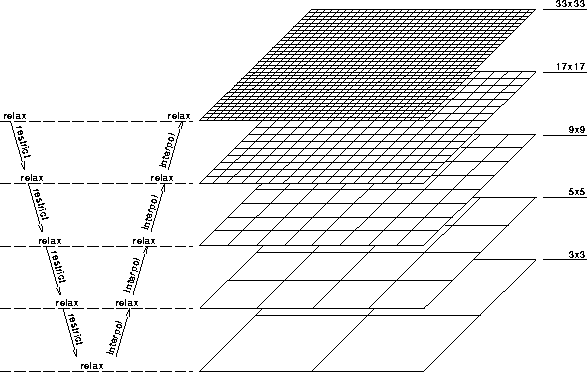
\includegraphics[scale=0.35]{img/02/multigrid.png}
\caption{\textbf{Vue des différents niveaux de grilles.} Image extraite de \href{http://MGNet.org}{MGNet.org} }
\label{Vue des différents niveaux de grilles}
\end{center}
\end{figure}	

\begin{figure}[htbp]
\begin{center}
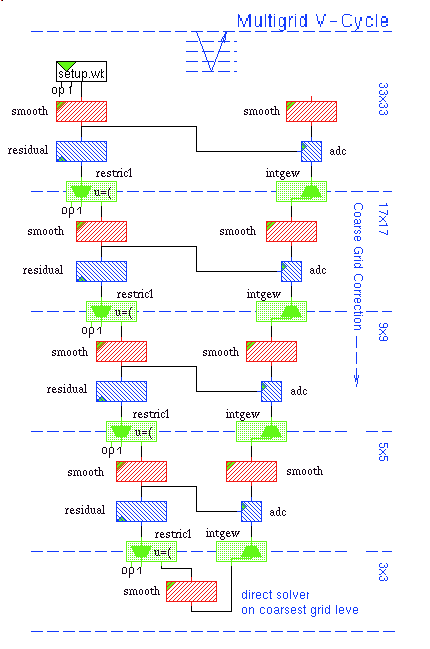
\includegraphics[scale=0.35]{img/02/Vcycle.png}
\caption{\textbf{Description du V-cycle.} Image extraite de \href{http://MGNet.org}{MGNet.org}}
\label{Description du V-cycle}
\end{center}
\end{figure}		

En jouant sur le nombre d'appels récursifs de la fonction, il est possible de créer différentes géométries de cycles. 
Un seul appel génère un cycle nommé cycle en V (fig. \ref{Description du V-cycle}), deux un cycle en W, etc... 

\subsection{Implémentation dans EMMA}
Dans EMMA, la potentiel est calculé par multigrille sur la grille coarse, et par Jacobi sur les niveaux raffinés.
La solution de la grille coarse étant injectée sur les niveau suivant, la solution est deja anticipée. 
Il en résulte une convergence rapide.

On prendra garde, lors de calcul en parallèle, a utiliser un niveau minimum de telle sorte que chaque processeurs dispose au minimum d'un oct.
Dans le cas contraire, le calcul ne donnera pas le bon résultat.

\subsection{Liste chaînée de particule}
La gestion des particules dans EMMA utilise le principe de la liste chaînée déjà abordée pour les OCT. %TODO ref
A chaque cellule est associée  un pointeur vers une particule de tète.
Si ce pointeur est NULL, la cellule ne contient pas de particule.
Les particules entrant dans cette cellule seront ajoutées a la liste chaînée.
On prendra garde a gérer cette liste au moment du raffinement et du déraffinement des cellules.



\subsection{Le pas de temps}

Le pas de temps sera calculer de telle sorte a respecter la condition de Courant.
Une particule ne doit pas se déplacer de plus d'une fraction de case a chaque pas de temps.


%	    dtloc=0.1*SQRT(2.*M_PI/(3.*(curoct->cell[icell].gdata.d+1.)*aexp));
%\begin{equation}
%
%\end{equation}



%%%%%%%%%%%%%%%%%%%%%%%%%%%%%%%%%%%%%%%%%%%%%%%%%%%%%%%%%%%%%%%%%%%%%%%%%%%%%%%%%%%%%%%%%%%%%%%%%%%%%%%%%%%%%%%%%%%%%%%%%%%%%%%%%%%%%%%%%%%%%%%%

\clearpage
\section{Le solveur hydrodynamique et la physique baryonique}

%solveur hydro
%partie la plus intensive en calcul


En cosmologie, le gaz est principalement soumis a deux forces : la pression et la gravité.
Comme nous l'avons vu plus tot, L'Univers est consitué d'une grande quantité d'Hydrogene et d'Helium sous forme gaseuse.
La physique du gaz est régie par les equations d'Euler auto-gravitantes :

\begin{equation}
\begin{cases}

{ \frac{ \partial \rho }{ \partial t } + \nabla \cdot (\rho v) = 0}, \\
\\
{ \frac{ \partial }{ \partial t } (\rho v) + \nabla \cdot (\rho v \otimes v ) \nabla p = -\rho\nabla \phi }, \\
\\
{ \frac{ \partial e }{ \partial t } + \nabla \cdot [ \rho v (e+p/\rho) ] = -\rho v \cdot \nabla \phi },

\end{cases}
\end{equation}
\label{eq:hydro}

Ce set d'équation peut être réécris sous la forme:

\begin{equation}
U+F(U) = 0,
\end{equation}

avec:
\begin{equation}
U=
\begin{cases}
{ \rho}\\
{ u}\\
{ v}\\
{ w}\\
{ E}
\end{cases}
,
F(U)=
\begin{cases}
{ \rho u}\\
{ \rho u^2+p}\\
{ \rho uv}\\
{ \rho uw}\\
{ u(E+p)}
\end{cases}
\end{equation}

Pour suivre l'évolution de ce gas nous allons le considérer comme parfait et monoatomique.

L’équation d'état du gaz sera donc:
\begin{equation}
p=\rho k T, 
\end{equation}
avec $k=1.38064852 \cdot 10^{-23} \left[ \mathrm{m^2 \cdot kg \cdot s^{-2} \cdot K^{-1}} \right] $ la constante de Boltzmann.


\subsection{Le probleme de Riemann}
L'idée est de décomposer le domaine en cellules dans lesquelles les grandeurs seront localement constantes. (Piecewise constant approximation)
On utilisera ensuite les equations d'Euler pour résoudre localement le problème de Riemann a chaque interfaces de cellule.
Nous aurons donc accès aux flux de matière et d'énergie entre les cellules pour pouvoir calculer l'état suivant  


Le problème de Riemann consiste a considérer l’évolution d'un system d’équation différentielles a partir d'une condition initiale.
En aillant l’état d'un système régis par des equations différentielles un instant donné, qu'elle sera sont évolution?

\begin{itemize}
\item PDE
\item IC
\item BC
\end{itemize}

\subsection{La discretisation du probleme.}


Contrairement a la résolution de l’équation de Poisson, il n'est plus possible d'utiliser une discrétisation des dérivées a l'aide d'un différence finie centrée.
Nous allons rapidement voir pourquoi dans cette section.


Une différence finie centrée peut être décomposée en deux différence finies : 
\begin{equation}
\frac{d u}{dx} \approx \frac{u_{i+1}  + u_i}{\Delta x} 
\end{equation}

\begin{equation}
\frac{d u}{dx} \approx \frac{u_i  + u_{i+1}}{\Delta x} 
\end{equation}



Considérons que nous voulons résoudre l'équation :
\begin{equation}
\frac{du}{dt} + a\frac{du}{dx} = 0
\end{equation}

Dans le premier cas, la discrétisation pourra s'écrire : 
%la propagation d'une onde a la vitesse $a$ pourra être discrétisée en utilisant.


\begin{equation}
\frac{u_i^{t+1} + u_i^t }{\Delta t}   +a \frac{u_{i+1}^t  + u_i^t}{\Delta x} = 0
\end{equation}


\begin{equation}
u_i^{t+1}  = u_i^t +  c \left( u_{i+1}^t  + u_i^t \right) 
\end{equation}

ou : 

\begin{equation}
c= \frac{a \Delta t}{\Delta x},
\end{equation}
est le nombre de Courant


A l'aide d'une analyse de von-Neumann (cf \cite{toro1999riemann}), on montre que la stabilité de ce schéma dépend du signe de a, la vitesse de propagation de l'onde.

\begin{itemize}
\item si a est positif, ce schéma est conditionnellement stable (la condition étant que la condition de Courant soient respectée : $0<c<1$) .
Ce schema est appélé méthode UPWIND.

\item A l'inverse on montre que que dans le cas de la seconde différence finie, le schéma est inconditionnellement instable. 
Ce shema est appelée méthode DOWNWIND.
\end{itemize}

Seule la méthode upwind permet de suivre correctement la propagation d'onde.
Le problème est qu'a trois dimension, il est impossible de respecter cette condition pour un système quelconque.
% déterminer dans quelle direction se propage une onde quelconques.


De plus il a été montré que cette méthode n'est pas conservative, et qu'elle était incapable de suivre les chocs (fortes discontinuités)

\subsection{Méthode de Godunov}


Godunov  \cite{MR0119433} a répondu a ce problème.

methodes conservative

introduction aux volumes finis
consiste a estimer le flux aux interfaces des cellules.


%\subsection{discretisation}
\begin{equation}
 \frac{\partial U}{\partial t} + \nabla \cdot (F(U)) = S(U), 
\label{eq:rad_generale}
\end{equation}

avec $U$ le vecteur des quantité conservées, $F$ la fonction de flux, et $S$ le terme source. Pour la résolution du transport des photons (sans terme source), on retrouve :

\begin{equation}
\frac{ u^{t+1}_i - u^t_i }{\Delta t} + \frac{ F^t_{i+1/2} - F^t_{i-1/2} }{\Delta x} =0,
\label{eq:rad_solver}
\end{equation}

ou $F^t_{i+1/2}$ et $F^t_{i-1/2}$ sont les flux numérique intercellules, une estimations des flux physique.

$F^t_{i+1/2}$

\subsection{Méhtode HLL et HLLC }
La méthode de HLL Harten, Lax et van Leer 
recalculation des flux entre les cellules

\subsection{MUSCL}
Monotonic Upstream-Centered Scheme for Conservation Laws (van Leer, 1979)
Consiste a considerer une valeur dans la cellule, non plus constante mais variable.
Cette variation est interpolée linéairement
%En utilisant la méthode de pente.

\subsection{Minmod}



\subsection{Le pas de temps}

Le pas de temps respecte encore une fois la condition de courant.

\begin{equation}
\frac{dx * CFL }{3*(max(v) + c_s)}
\end{equation}

avec $cs = \gamma P/\rho$

%%%%%%%%%%%%%%%%%%%%%%%%%%%%%%%%%%%%%%%%%%%%%%%%%%%%%%%%%%%%%%%%%%%%%%%%%%%%%%%%%%%%%%%%%%%%%%%%%%%%%%%%%%%%%%%%%%%%%%%%%%%%%%%%%%%%%%%%%%%%%%%%
\section{Le solveur radiatif}
\label{sec:rad_solver}

Il existe deux grandes famille de code de transfert de rayonnement.
\begin{itemize}
\item La première famille utilise une représentation très physique de la lumière, et simule la radiation a l'aide de rayons se propageant dans l'espace.
CRASH \citep{2003MNRAS.345..379M}, C$^2$RAY\citep{2006NewA...11..374M}.
Ce type de code utilise une principe qui se rapproche physiquement de la vraie nature de la lumière.
Chaque source lance un certain nombre de groupe de photon, qui vont se propager et interagir avec le milieu.
Plus les sources sont nombreuses, plus le nombre de groupe de photons a suivre devient important, et plus le cout numérique l'est également.

\item La seconde, celle utilisée dans EMMA, repose sur le principe de considérer la lumière comme un fluide. \citep{gnedin_multi-dimensional_2001, aubert_radiative_2008}.
Ces méthodes dites méthodes aux moments utiliseront donc les même concepts que le solveur hydrodynamique, mais avec un système initial d'équations différentes. 
EMMA utilise une approximation du moment au premier ordre, son solveur repose sur l'\textit{approximation M1} \citep{levermore_relating_1984}.
Son principal avantage est que le coût numérique est indépendant du nombre de sources.
\end{itemize}

Ce solveur se déroule en deux temps.
Premièrement, il faut calculer la propagation du rayonnement, on appelles cette étape \textit{le transport} des photons.
Deuxièmement, il faut le couplage entre le rayonnement et le gaz, c'est a dire calculer l'impact \textit{chimie} du gaz.


\subsection{Les équations du transfert du rayonnement}
\begin{equation}
\frac{1}{c} \frac{\partial I_\nu}{\partial t} + \vec{n}\cdot \vec{\nabla} I_\nu = \eta_\nu - \kappa_\nu I_\nu 
\end{equation}
Avec: $I_\nu(\vec{x},\vec{n},t)$ l'intensité spécifique,
$\eta_\nu(\vec{x},\vec{n},t)$ la source de rayonnement,
le coefficient d'absorption $\kappa_\nu(\vec{x},\vec{n},t) = \sigma_\nu n_H$, 
$\sigma_\nu$ la section efficace de photo-ionisation de l'hydrogène neutre et $n_H$ la densité d'hydrogène neutre


\begin{equation}
\begin{cases}

\frac{ \partial N_\nu }{ \partial t } + \vec{\nabla} \cdot \vec{F}_\nu = -\kappa_\nu c  N_\nu + S_\nu,\\

\frac{ \partial \vec{F} }{ \partial t } + c^2 \vec{\nabla} P_\nu = -\kappa_\nu c \vec{F}_\nu ,

\end{cases}
\label{eq:densite_energie}
\end{equation}
Représentant respectivement les moments d'ordre 0 et 1 de $I_\nu$ avec:
$\vec{F}_\nu$ le flux radiatif, 
$P_\nu $ la pression radiative
et $S_\nu = \dot{N}_\nu^* + \dot{N}_\nu^{rec}$ le taux d’émission de photon due aux sources $\dot{N}_\nu^*$ et a la recombinaison $ \dot{N}_\nu^{rec}$


\subsection{Relation de fermeture et approximation M1}
La fermeture du système se fait par l’intermédiaire de l’équation d’état, avec $D$ le tenseur d’Eddington :

\begin{equation}
 P_\nu = D N\nu ,
\label{eq:fermeture}
\end{equation}

où D est approximé par le modèle M1 \citep{levermore_relating_1984}%,gonzalez2005} :

\begin{equation}
\begin{cases}

D = \frac{ 3\chi -1 }{2} \mathbb{1} + \frac{ 1 - \chi }{2} \vec{n} \otimes \vec{n} , \\
\\
\chi(\vec{f}_\nu) = \frac{ 3+4 |\vec{f}_\nu|^2 }{5+2\sqrt{4-3|\vec{f}_\nu|^2}} , \\
\\
\vec{f}_\nu = \frac{ \vec{F}_\nu }{c N\nu }  ,

\end{cases}
\label{eq:tenseur}
\end{equation}


\subsection{Pas de temps et vitesse de la lumière réduite}

Condition de Courant radiative : $ c \leq \Delta x / \Delta t $.
Le pas de temps est donc plusieurs ordres de grandeur plus petit que celui de l'hydrodynamique.

%Pour compenser cette 

Les simulation cosmologique utilise l'approximation Newtonienne: les processus entrant en jeux on des vitesses très inférieurs a celle de la lumière.
L'idée est de diminuer la vitesse de la lumière dans le code tout en restant dans le domaine de l'approximation newtonienne.
Cette idée est développée en détails dans la section %TODO ref



\subsection{La chimie}

La chimie fait le lien entre le solveur radiatif et le solveur hydrodynamique.
C'est a ce moment qu'est appliquée l'énergie apportée par la radiation au gaz.
gestion du refroidissement/ de la température/ énergie interne
Contrairement au transport, la chimie est non conservative.

Densité de photons
\begin{equation}
\frac{dN}{dt} = S - c \sigma_N n_H N + \left( \alpha_A(T)  - \alpha_B(T) \right) x^2n_0^2
\end{equation}

Flux de photons
\begin{equation}
\frac{dF}{dt} = - c \sigma_N n_H F
\end{equation}

État d'ionisation
\begin{equation}
\frac{dn_H}{dt} =  \left( \alpha_A(T)x^2  - \alpha_B(T)x (1-x) \right) n_0^2 - c \sigma_N n_HN
\end{equation}


Énergie interne
\begin{equation}
\frac{de}{dt} = c n_H \Sigma_E N - \Lambda_{(n_0,x,T)}
\end{equation}


Les taux de réaction chimique $\alpha_A(T)$, $\alpha_B(T)$ et $\beta_(T)$ sont repris de tables de \cite{theuns_p^3m-sph_1998}.
Les sections efficace d'interactions viennent de \cite{hui_equation_1997}.

Les processus chimique agissant sur des échelles de temps courtes par rapport au transport des photons, le pas de temps sera plusieurs ordres de grandeurs plus faible.
En pratique, a chaque pas de temps radiatif, on effectuera un sous-cyclage sur le pas de temps chimique.
Après chaque pas de temps chimique, la variation d’énergie est calculée. 
Si celle ci est supérieure a 10\%, le pas de temps est divisée par 2 et l'étape courante est recalculée. (cf \cite{rosdahl_ramsesrt_2013}) 

Étant donné que le processus chimique sont uniquement local (ils ne dépendent pas de l'état des cellules voisines) et que la quantité de calcul est relativement importante, le portage du solveur chimique sur GPU est très intéressant du point de vue accélération.


\subsection{Groupes de photons}
\label{sec:groupedephotons}

Il n'est pas possible avec la méthode au moment de considéré directement un spectre d'émission.
Le spectre doit être discrétisé, c'est a dire qu'il devra être découpé en un certain nombre de groupe, et chaque groupe disposera des caractéristique moyenne de sa portion du spectre.
Le problème est que chaque groupe de photon devient un fluide a simuler. 
L'augmentation du nombre de groupe devient vite coûteux en terme de temps de calculs.

%Les caratéristiques des photons\\

Nous aborderons la mise en place du multi longueur d'onde dans la section %TODO ref



\chapter{Matériel et parallélisme}

Nous avons maintenant un apercu de la quantité de calcul a exécuter.
De plus, les simulations cosmologiques ont pour principal défi de simuler d'important volume d'espace avec la meilleure résolution possible.
Le défis des simulations de la réionisation est qu'elles doivent simuler un volume d'univers suffisant pour être représentatif ( $\approx 100$ Mpc selon \cite{iliev_cosmological_2006}) tout en résolvant la formation stellaire (échelle $<1$ pc).
Nous verrons dans la prochaine partie que nous sommes encore loin de pouvoir résoudre la formation stellaire dans ce type de simulations. %TODO ref
Nous avons vu que l'amélioration de certain algorithme (passage de grilles fixe a grille adaptative, intégration du potentiel plutôt que somation Ncorps directe, etc) a permis d'augmenter significativement la taille des simulations a puissance de calcul identique, mais le principal facteur limitant reste au niveau du matériel.

\subsection{Loi de Moore et simulations}
La loi de Moore \citep{moore1965cramming} propose un doublement du nombre de transistor par circuit intégré tout les 18 mois environs. (Fig \ref{fig:moore})
Comme la puissance de calcul est étroitement liée au nombre de transistor par cœur, la taille -- le nombre d'éléments de résolution -- des simulations, suis également cette croissance exponentielle (Fig. \ref{fig:taillesimu}).

\begin{figure}[bth]
        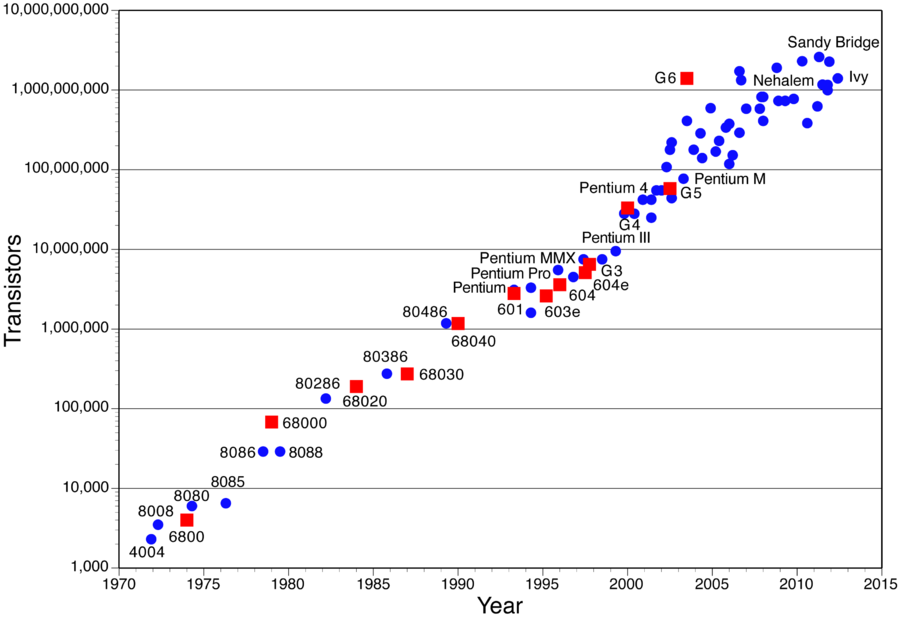
\includegraphics[width=.95\linewidth]{img/02/moorelaw.png} 
        \caption{Nombre de transistor par processeur en fonction du temps.
        Cette croissance exponentielle est connue sous le nom de loi de Moore}
 		\label{fig:moore}
\end{figure}

\begin{figure}[bth]
        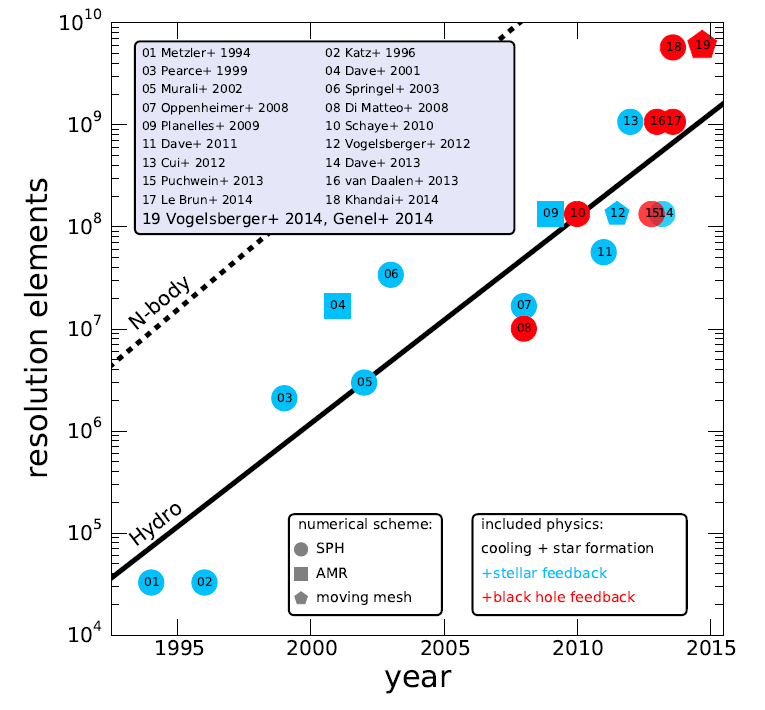
\includegraphics[width=.95\linewidth]{img/02/figure_simulations_with_time.png} 
        \caption{Tailles des simulations en fonction du temps.
        Il existe un lien directe avec la loi de Moore.
         Image illustris}
 		\label{fig:taillesimu}
\end{figure}


\subsection{Principes de parallélisation}

Comme on ne peux pas créer des processeurs aussi gros que ce que l'on le souhaite, la technique utilisée pour continuer a augmenter la puissance de calcul, consiste a en utiliser plusieurs en même temps.
C'est ce qu'on appelle le parallélisme.

Dans le cas des simulation cosmologique, la parallélisation est effectué en découpant l'espace a simuler en un certain nombre de sous domaines.
Chaque processus indépendant sera alors chargé de simuler un sous domaine.
Comme chaque sous domaine n'est pas isolé, mais appartient au même ensemble, les domaines vont devoir communiquer entre eux sur l'état de leurs voisin.
Nous verrons en détail comment est effectué ce découpage dans la section \ref{sec:parasoft}.
Mais voyons d'abord qu'elles sont les contraintes techniques de la parallélisation.

Il existe différent type de parallélisation définis par la taxonomie de Flynn \citep{Flynn:1972:COE:1952456.1952459}: 

\begin{itemize}
\item SISD Single Instructions on Single Data.
Aucun parallélisme, exécution d'une unique série d'instructions sur un unique flux de données.

\item SIMD Single Instructions on Multiple Data.
Exécution d'une unique série d'instructions sur différents flux de données.
C'est le principe de fonctionnement des GPU.

\item MISD Multiple Instructions on Single Data 
Exécution de différentes série d'instructions sur un seul flux de données.

\item MIMD Multiple Instructions on Multiple Data.
Exécution de différentes série d'instructions sur différents flux de données.
C'est l’architecture la plus utilisé aujourd'hui, et celle qui nous intéresse ici.
Le type MIMD est lui même découpé en deux sous ensembles : 

\begin{itemize}
\item On dit que la mémoire est \textit{distribuée} quand les threads on leur propre espace mémoire dédié.
Les principales machines que j'ai pu rencontrer utilise un modèle MIMD a mémoire distribuée.

\item On dit que la mémoire est \textit{partagée} quand plusieurs threads ont accès au mème espace mémoire.
\end{itemize}
\end{itemize}

Il existe plusieurs niveau de parallélisation, au niveau matériel.
Par exemple, un processeur actuel dispose de plusieurs cœurs, capable de géré chacun un processus (voir 2 dans le cas de l'hyperthreading).
Il est possible d'avoir plusieurs processeur au sein d'un même ordinateur.
Et il est possible d'utiliser conjointement plusieurs ordinateurs.
Ce qui nous mène a la notion de centre de calcul.

\subsection{Les calculateurs}

La production de simulation cosmologique a haute valeur scientifique ne se fait pas sur un simple ordinateur personnel.
Pour réaliser de telle simulations, nous (les simulateurs) utilisons des centres de calcul.
A la manière d'un télescope pour les observateurs, les supercalculateur sont les outils principaux des simulateurs.
Et a la manière des plus gros télescopes, ces calculateurs sont gigantesques.

La figure \ref{fig:titan} présente le calculateur TITAN du Oak Ridge Leadership Computing Facility sur lequel ont été éxécuté les simulations CODA \citep{ocvirk_cosmic_2015}.
TITAN a été classé quatrième plus puissant calculateur au monde selon le cite top500.org (cf \ref{tab:top500}).

\begin{figure}[bth]
        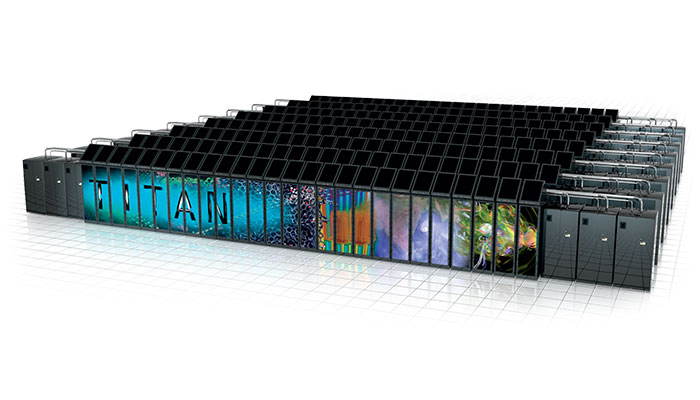
\includegraphics[width=.95\linewidth]{img/02/titan.jpg} 
        \caption{Supercalculateur Titan OLCF.
        ou ont été exécutés les simulations CODA}
 		\label{fig:titan}
\end{figure}

\begin{table}[bth]
\begin{tabular}{ l l l l }
\hline 
Système & Pays & nb de cœurs & TFlop/s (peak) \\
\hline 
Sunway TaihuLight & Chine & 10,649,600 & 125,435.9 \\ 
Tianhe-2  & Chine & 3,120,000 & 54,902.4 \\ 
Piz Daint  & Suisse & 361,760 & 25,326.3 \\ 
Titan  & États unis & 560,640 & 27,112.5 \\ 
Sequoia  & États Unis &1,572,864 & 20,132.7 \\ 
\end{tabular} 
\caption{Les 5 super calculateurs les plus puissants du top500 de Juin 2017, source : www.top500.org}
\label{tab:top500}
\end{table}


Ce type de calculateur est composé d'un certain nombre de nœud (ordinateur) qui communique entre eux par l'intermédiaire d'un réseau.

D'une manière générale, plus des composants sont physiquement éloignés, plus leurs communications seront lente (cf \ref{tab:debits})


\begin{table}
\begin{tabular}{ l l }
\hline 
Interface  & Débit théorique \\
\hline 
Cache L1 & $\approx$ 700Go/s \\
RAM & $\approx$ 20 Go/s \\ 
PCIE 16x & $\approx$ 16 Go/s \\
InfiniBand & $\approx$ 5 Go/s \\
SSD & $\approx$ 600 Mo/s \\
HDD & $\approx$ 100 Mo/s
\end{tabular} 
\caption{Ordre de grandeur des débits théorique des différentes interface rencontrées lors de l'exécution d'un code HPC}
\label{tab:debits}
\end{table}


En principe, la mémoire est partagé au sein d'un nœud, et distribuée sur le réseau.
C'est a dire que tout les processus au sein d'un même nœud pourront communiquer par l'intermédiaire de la RAM, ce type de communications est rapide.
Pour les communications entre les nœuds, l'information devra passer par le réseau, ce type de communications est donc plus lent.
Durant le développement d'un code HPC, on cherchera a minimiser les communications par le réseau.



%Les cœurs au sein d'un même CPU pourront communiquer entre eux de faible quantité de données par l’intermédiaire du cache, ou en passant par la RAM pour les volumes plus importants.



%Proche d'un ordinateur personnel un nœud est composé d'une carte mère sur laquelle est relié entre autres, un ou plusieurs processeurs (CPU), une certaine quantité de mémoire RAM et parfois une carte graphique (GPU)
%Chaque CPU dispose d'un certain nombre de cœurs, et chaque cœurs est capable d'exécuter un certain nombre de processus ou thread (généralement 1, parfois 2 dans le cas de l'Hyperthreading)

%
%Une fois les processus et les domaines identifiés il existe différentes facons de faire dialoguer les processus entre eux.
%La principale distinction viendra généralement de si les threads sont exécutés par un meme noeud ou non.
%
%, cad par exemple que si le thread 0 déclare une variable X, le thread 1 aura aussi accès a cette variable . 
%OpenMP est une API permettant ce  genre partage de mémoire.
%
%
%Si les threads sont exécutés sur un même nœud on aura tendance a utiliser un schéma a base de mémoire partagée.
%
%Dans le cas ou les threads sont exécutés par des processeurs étant physiquement éloigné, ie sur des noeuds différents, les communications doivent passer par un réseau de communication reliant les noeuds.
%Il faudra utiliser dans ce cas une autre API pour explicitement envoyer et recevoir des paquets d'information
%L'API la plus communément utilisée pour ce genre de communication est Message Passing Interface MPI.
%
%
%
%\paragraph{Nœud :} Élément du centre de calcul relier par un réseau.
%
%La difficulté est de géré la façon dont les threads travaillent ensemble.
%En effet a chaque thread sera associé un domaine de calcul représentant une partie de l'espace a modéliser.
%De plus les domaine ne sont pas isolés et partage de l'information. 
%
%Nous sommes alors confronté a plusieurs problèmes: comment associer les threads aux domaines de calculs  et comment faire communiquer ces threads entre eux.
%
%
%
%Ces machines se composent d'un certain nombre de nœuds.



\subsection{Courbe de Peano-Hilbert}
\label{sec:parasoft}

%https://books.google.fr/books?id=sbQqBgAAQBAJ&pg=PA26&lpg=PA26&dq=peano+hilbert+mpi&source=bl&ots=HgSw0Jpf7d&sig=vXTb2JkDixd1gcDGANoARIYHAG0&hl=fr&sa=X&ved=0ahUKEwilofzKoerSAhUF6RQKHXzQDC4Q6AEIGjAA#v=onepage&q=peano%20hilbert%20mpi&f=false


%Warren et Salmon
Le découpage des domaines de calcul correspondants aux différents processeurs, utilise une courbe de Peano-Hilbert.
Ce type de courbes fractale a la particularité de remplir l'espace.
Mais aussi de passer par tout les points d'une grille.
Ainsi si l'on applique ce pavage aux cellules de notre grille, en associant un indice reliant un cellule a sa position sur la courbe de Hilbert.
Il suffit ensuite de découper la courbe en parties identique  pour 
Ainsi si l'on a par exemple  32 cellules a assigner sur 4 processeurs, la courbes sera découpée en 4 parties de 8 cellules.
Chacune de ces partie sera en suite assignée a un processeur.

Ce type de découpage minimise les interfaces entre domaine, en s'assurant d'une proximité spatiale entre tout les points de la courbe.
Elle minimise donc les communications entre processeurs.

\begin{figure}[bth]
        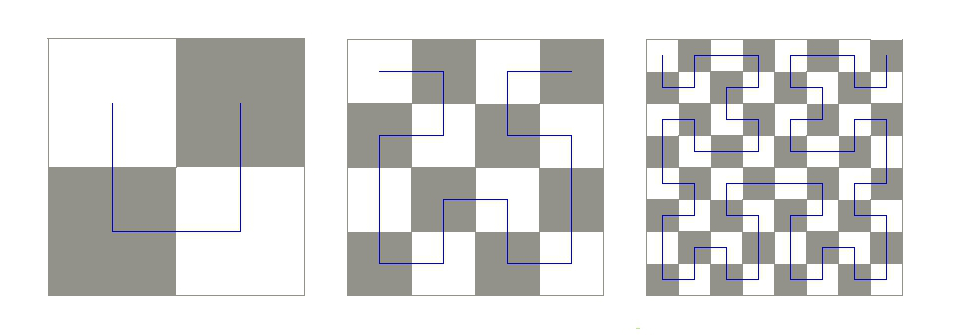
\includegraphics[width=.95\linewidth]{img/02/courbe_Hilbert.jpeg} 
        \caption{exemple de courbe de Hilbert. 
        %http://www.lifl.fr/~pmathieu/transform/fractales.html
}
 		\label{fig:hilbert}
\end{figure}

%
%\begin{figure}[bth]
%        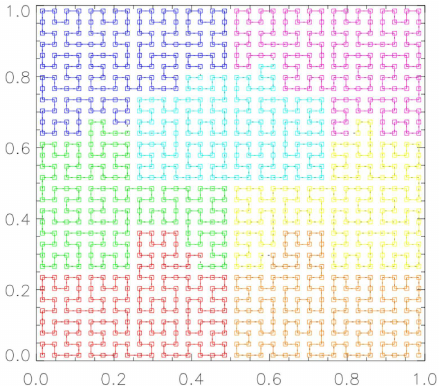
\includegraphics[width=.95\linewidth]{img/02/hilbert2.png} 
%        \caption{exemple de courbe de Hilbert. 
%%http://iopscience.iop.org/article/10.1086/590370/pdf 
%}
% 		\label{fig:hilbert2}
%\end{figure}


Dans l'état actuel du code, la courbe est calculée au debut de la simulation, et donc  seul la grille coarse est prise en compte.
De plus, la repartition des dommaines est statique et n'évolue pas au cour de la simulation.
Dans le cas ou un domaine raffine plus qu'un autre, la charge de travail y est plus importante.
Dans le futur, l'objectif serai de calculer la courbe de Hilbert sur la totalité des cellules feuilles.
Pour ainsi pouvoir refaire le découpage et donc équilibrer la charge entre les processeurs.
C'est ce qui s'appel le "load balancing".


\begin{figure}[bth]
        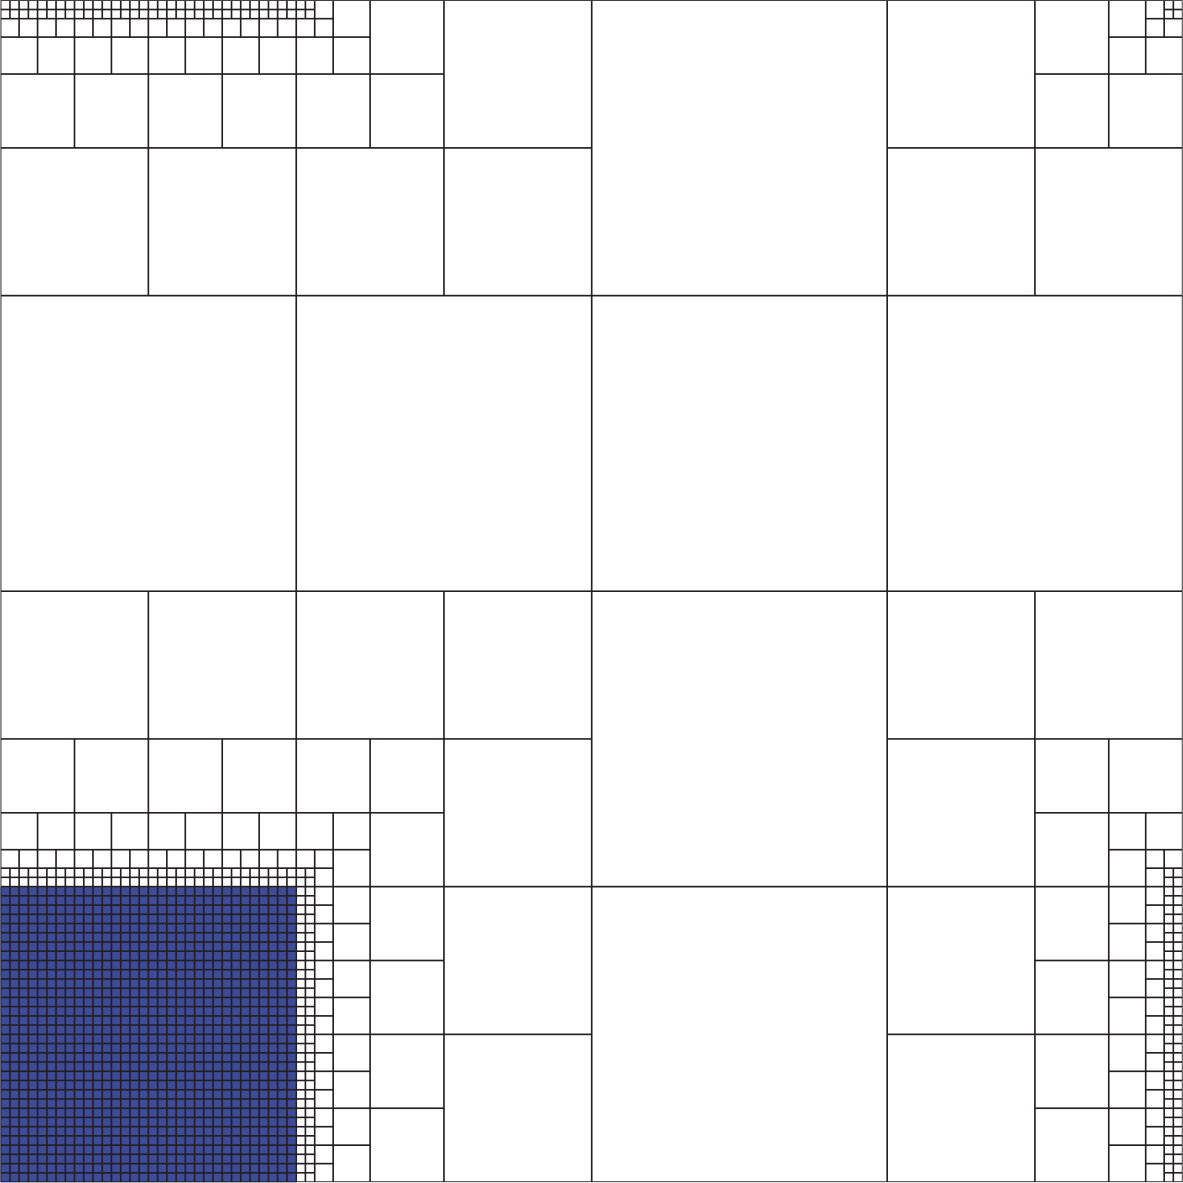
\includegraphics[width=.95\linewidth]{img/02/secteur.png} 
        \caption{Exemple de domaine de processeur généré par EMMA. 
        Chaque domaine représente une vue d'ensemble de la grille, a résolution dégradée.
}
 		\label{fig:hilbert2}
\end{figure}





%Je n'ai aucun doute sur le fait que dans les années a venir 


\subsection{GPU}

EMMA utilise un degré supplémentaire de parallélisation.
Les calcul de chaque domaines sont accéléré en utilisant les capacité parallèle des processeur graphic récents.
Les cartes graphiques, ou GPU (pour Graphics Processing Unit) ont été détourné de leurs utilisation principale d'affichage il y a une dizaine d'années.

A l'inverse des CPU actuels, qui disposent d'un nombre réduit de cœurs (8 coeurs hyperthreadé pour un Intel® Xeon® X7560 de Curie et 16 cœurs pour un AMD Opteron 6300 de TITAN) les GPU dispose d'une nombre beaucoup plus important de coeurs (Fig \ref{fig:cpugpu})
Par exemple la NVIDIA Tesla k40c dispose de 2880 coeurs.

\begin{figure}[bth]
        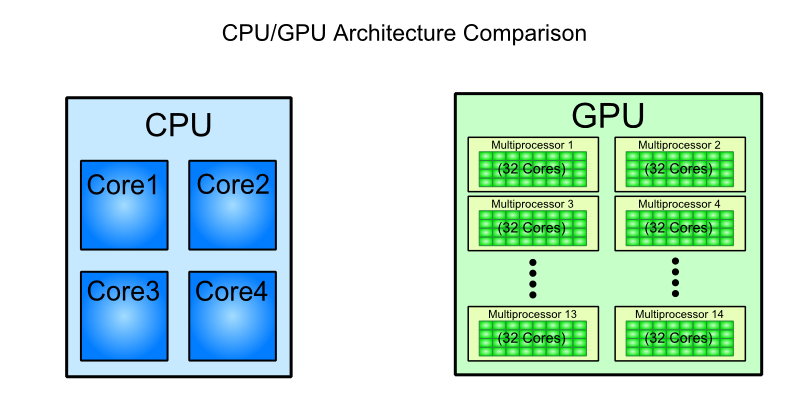
\includegraphics[width=.95\linewidth]{img/02/cpu_vs_gpu.png} 
        \caption{Comparaison CPU/GPU. Une CPU dispose d'un nombre réduit de cœurs capables d’exécuter des opération complexe. A l'inverse un GPU dispose d'un grand nombre de coeurs pouvant éxécuter un grand nombre d'opérations simples en parallèle}
 		\label{fig:cpugpu}
\end{figure}


Un CPU peux exécuter des taches différentes sur chacun de ses coeurs (MIMD).
Les GPU utilise un mode de parallélisation de type SIMD.
Ces unités de calculs sont  efficaces dans le traitement d'un grand nombre d'information en parallèle.
Elle sont donc toutes indiqués dans le cas des simulations numérique ou il s'agit d'appliquer un traitement identique a chaque cellules de la grille.

Il existe 2 principaux avantage aux GPU par rapport aux CPU.
Premièrement leurs meilleurs ratio puissance de calcul sur coup (flop/€).
Et également un meilleur ratio puissance de calcul sur puissance élcetrique (flop/W) ce qui reduit les besoins de refroidissement et permet des économies supplémentaires.


%
% et de 12Go de mémoire et a une puissance de calcul de 4.3 Tflop/s en simple precision.
%
%
%Intel® Xeon® X7560 -> TDP 130 W -> 76 Gflop/s (crete)
%
%
%IBM A2 (sequoia) -> 204 Gflop/s -> TDP 55W

 

Cependant CPU et GPU sont indissociable est il faut les utilisé conjointement pour tirer le meilleurs partis des capacitées de calcul offerte par une machine hybride.

Une code hybride est découpé en deux parties, une partie sequentielle exécuté sur le CPU et une partie paralélle exécuté sur le GPU.
On tirera le maximum des capacités d'accélération d'un GPU avec un code qui est autement parallélisable.
%En effet si l'on peux éspérer



La programmation sur carte graphique utilise une approche proche du concept de mémoire distribuée.
Cad que la carte graphique GPU et le processeur central CPU ont besoin de communiquer.
Leurs espaces mémoire ne sont pas commun.

%Or a l'heure actuelle cette communication utilise une interface relativement lente (PCI express) qui rend coûteuse la communication. 
Il faut donc que la quantité de calcul effectués par la carte soit suffisante pour rentabilisé la communication.


plus dur a programmer, performance dépends du problème.





\subsection{Les communications CPU/GPU}

Les CPU sont capable d'accéder rapidement aux informations en mémoire, quel que soient leurs organisation.
Le GPU sont sensibles à la segmentation des données.
C'est à dire que les calculs sur GPU seront performants si les données sont organisées de facons a ce que leur accés memoire consecutifs soient physiquement proches.
Prenon l'exemple d'une différence finie. 
Pour calculer le nouvel etat d'une cellule, il est necessaire de connaitre sont état actuel, et celui de sa voisine.
L'accès mémoire sera plus rapide si l'information est situer sur un espace mémoire adjacent.

La difficulté est que l'arbre AMR ne respecte pas cette organisation, et peut être extremement fragmenté.
Dans EMMA le choix a été fait d'organiser les données sur le CPU, avant de les envoyer sur le GPU (opération de "gather").
Les calculs sont effectués sur le GPU avec une structure memoire adequate, puis rapatriée et remises dans l'arbre par le CPU ((opération de "scatter") (cf Fig. \ref{fig:gatherscatter})

Ce choix est motivé par le fait qu'une structure mémoire bien organisée peux amener a des gains conséquents.
Par exemple dans ATON %TODO ref
un code de transfert radiatif sur grille fixe, le gain GPU est de l'ordre de 80.

Le pari est ici que la perte de temps genérée par les opérations de gather/scatter sera compensé par l'accélération du GPU.


\begin{figure}[bth]
        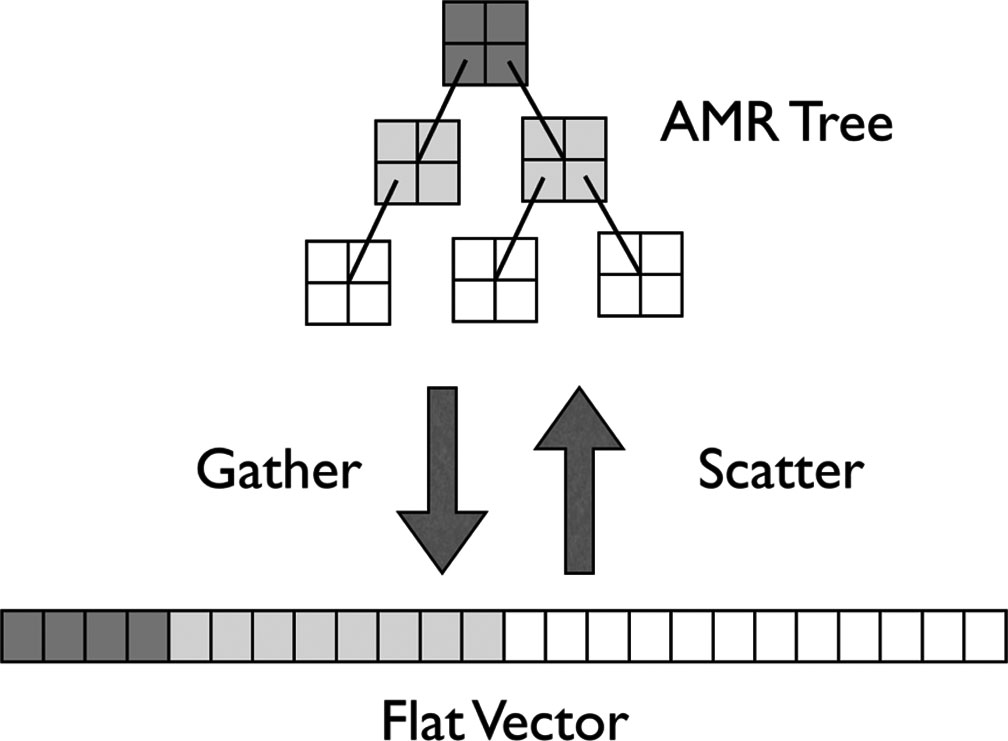
\includegraphics[width=.95\linewidth]{img/02/gatherscatter.jpg} 
        \caption{Transition entre la structure en arbre de l'AMR et la structure en vecteur de calcul.
}
 		\label{fig:gatherscatter}
\end{figure}


En pratique l'opération de gather consiste a rassembler toutes les informations necessaire au calcul de l'état d'une cellule.
Par exemple pour le calcul du potentiel (cf ) %TODO ref
les données necessaires seront: la densité locale, le potentiel local, le potentiel des 6 cellules voisines des axes principaux.
Ces données sont rassemblées dans une structure, et stockées dans un tableau.
Cette opération sera réalisée pour chaque cellule de la grille.

On peut observer ici que les copies ont beaucoup de redondance.
Une cellule d'interet + copie de 6 cellules, le ratio est de $1/6$.
Le potentiel d'une cellule sera copié sept fois sur le GPU.

Ces multiples copies diminue grandements les performances et en font l'une des principales limitations à l'accélération globale du code.
Toute fois, même dans cet état, l'éxécution s'en trouve accélérée d'un facteur $\approx 3$ par rapport à la version CPU.

Dans le but de réduire le nombre de copies et accélérer l'éxécution du code, j'ai modifié les opérations de gather/scatter pour diminuer la redondance des copies.
Au lieu de traiter les cellules unes par unes, l'idée est de traiter les octs.
Dans ce cas les cellules sont traité par 8 et les voisinages au sein d'un oct peuvent être directement traité.
On copie donc 8 cellules d'interet et 4 cellules de bord par face du cube, soit 24 cellules.
Le ratio passe donc a $8/24 = 1/3$ la quantité de copies redondante a donc été diminuée par 2 par rapport au cas précédent.

Vu que la surface d'un cube augmente avec le caré de son coté, alors que son volume augmente avec son cube, plus grand sera la nombre de cellule d'interet, meilleur sera la ratio.
En étendant ce principe, j'ai dévellopé une méthode qui permet de manière récursive d'envoyer une portion d'AMR contenue dans un OCT de niveau arbitraire.

Cependant les résultats ne sont pas a la hauteur des espérances, et l'accélération n'est pas proportionnelle au ratio de données utiles.

IL existe cependant des pistes pour améliorer ce goulot d'étranglement.
La plus prométeuse semble être de suprimer complétement les copies en placant la totalité de l'arbre directement sur la carte.
Dans ce cas, c'est le GPU qui devra gérer l'evolution de l'arbre. 
%Le CPU étant tres efficace pour ce genre d'opération, il semble

Une autre possibilité est de séparer la gestion de l'arbre de la physique.
En l'état actuel, les données physique sont stockées en mémoire avec la même structure que l'arbre.
L'idée serait de stocker dans l'arbre, des indices de cellules permettant de retrouver l'information physique dans des vecteurs plat (cf Fig. \ref{fig:gatherscatter}).
Ainsi les vecteurs pouraient être en premanance sur le GPU, et seul l'information sur leurs position dans l'AMR devrait être transmise.
Un grand nombre de copies seraient alors évitées.



%Copies asynchrones




\subsection{Gestion des entrées sortie}

Si l'on se réfère a la table \ref{tab:debits} on observe que les débits d'accès disques sont les plus faible.
Et étant donné la quantité de données en jeu, une bonne gestion des Entrées/Sorties peut donc permettre un gain de temps appréciable.

Les entrées sorties sont des étapes relativement longues et l'écriture sur disque d'une telle quantité de données demande du temps et ralentit l'exécution de la simulation.
De plus, ces données sont généralement calculé sur des machines distante et leurs rapatriement sur des machine locales peut également être coûteux en temps.
Il a fallu plusieurs mois pour rapatrier localement les données générées par la simulation CODA.

De plus améliorer la compacité des données permet également de gagner du temps au moment du transfert vers des machines distante, ou simplement au moment de la lecture

%analyse a distance

%le feedback CODA\\
%grosse quantité de données\\

Il a fallut plusieurs mois pour rapatrier les données de CODA de TITAN aux états unis vers Strasbourg

CODA II EMMA (voir partie \ref{sec:CODAEMMA})
L'objectif durant ma thèse était de réaliser une simulation de la réionisation avec un nombre de particule de matière noire (et donc une grille coarse) de $2048^3$.
Et si il faut calculer ces données, il faut également les stocker, cad les écrire sur disque dur.

\begin{itemize}
\item Pour les particules:
En considérant qu'un flottant est codé sur 8 bits, chaque champs représente 8Go.
Il y a une dizaine de champs en sortie (3 positions, 3 vitesses, etc): environs 80Go

\item Pour la grille :
En considérant qu'approximativement la quantité de cellule est multipliée pas 3 a cause du raffinement  chaque champ physique (densité, température, composante de la vitesse, etc..) représente environ 24Go de donnée.
Il y a au total un cinquantaine de champs physique nécessaire a l'exécution de la simulation mais en pratique environ une vingtaine en sortie.
Chaque écriture représente donc 500Go pour la grille.

\item Pour les étoiles:
c'est très variable car dépend directement du nombre d'étoile a l'instant donné, qui dépend lui même du paramètre de résolution.
\end{itemize}

Soit au total environ 600Go par pas de temps.

Mais on voudrait évidemment avoir accès a l'état de la simulation a différents instant.
Cette simulation a au final générée 170 snapshot.
Au final le volume de donnée de la simulation représente environs une centaine de tera octets.



Dans l'ancien modèle de données d'EMMA,  
L'intégralité de l'octree était écrit.
Les oct étaient écrit les uns a la suite des autres avec toutes l'information qu'ils contenaient.
L'information étaient exacte, mais le volume de données était considérable.
De plus chaque processeur écrivait un fichier indépendant, ce qui pouvait rapidement faire exploser le nombre de fichiers.


Le nouveau modèle que j'ai implémenté se base sur une notion de tableau de champs.
Les processeurs écrivent conjointement dans le même fichier, le nombre total de fichiers ne dépend plus du nombre de processeurs sur lequel a tourné la simulation.
Les écriture sont réalisées en parallèles grâce a l' utilisation de la librairie hdf5
Selon file-système des calculateurs, il est possible d'avoir un nombre limité de fichier par utilisateur.
Seules les feuilles (les cellules non raffinées) sont écrites sur le disque.
Ce qui permet de réduire la redondance des données, mais ne contrepartie il est nécessaire de reprojeter la grille au niveau voulu 
Chaque fichier représente un champ physique.
Lors d'un transfert entre machine, il est possible de ne rapatrier que les champs nécessaire, et ainsi économiser de la bande passante.
Chaque cellule est considérée comme une particule d'une certaine taille.

%TODO faire le lien avec \ref{fig:gatherscatter}

%Architecture des données 
%conception d'une organisation des données
%séparation des champs
%structure imposé par la gestion de l'AMR
%écriture parallèle

%\subsection{Potentiel d'optimisation EMMA}
%
%la forme des gathers/scatter
%optimisation matérielle -> les prochaines générations de GPU
%Opérations coarse sur grille non AMR.
%reformatage de l'arbre et découplage de la physique




%\begin{figure}[bth]
%        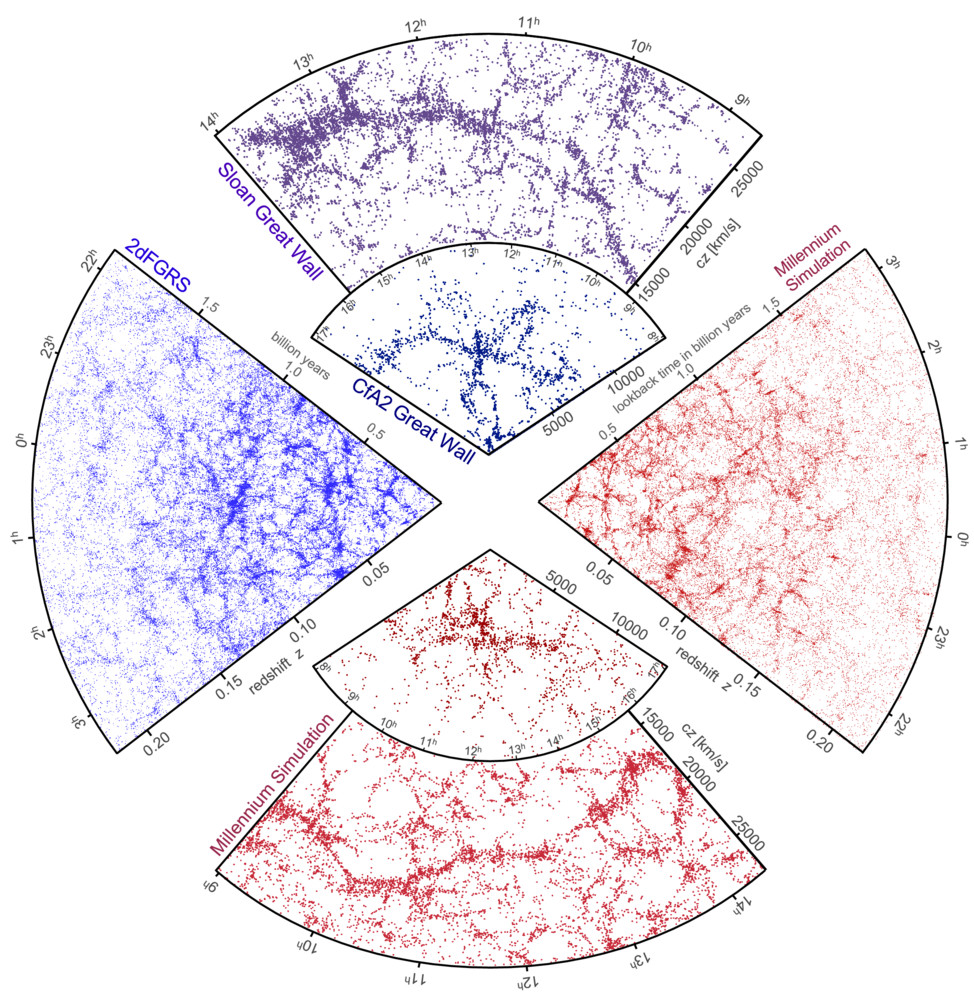
\includegraphics[width=.95\linewidth]{img/02/sdss_millenium.jpeg} 
%        \caption{ 
%%http://wwwmpa.mpa-garching.mpg.de/millennium/
%}
% 		\label{fig:}
%\end{figure}


\chapter{Matériel et parallélisme}
\label{sec:materiel}
%Nous avons a ce stade un aperçu du type de calcul a effectuer, essayons d'estimer . 
%De plus, les simulations cosmologiques ont pour principal défi de simuler d'important volume d'espace avec la meilleure résolution possible.

Le défis des simulations de la réionisation est qu'elles doivent simuler un volume d'univers suffisant grand pour être représentatif de la variance cosmique( $\approx 100$ Mpc selon \cite{iliev_cosmological_2006}) tout en résolvant la formation stellaire (échelle $<1$ pc).
En première approximation, il nous faudrait donc échantillonner un tel volume par $\left( \frac{100Mpc}{1pc} = 10^7 \right) ^3 = 10^{21}$ éléments.
Ce qui est totalement impossible à l'heure actuelle.
%Nous verrons dans la prochaine partie que nous sommes encore loin de pouvoir résoudre la formation stellaire dans ce type de simulations. %TODO ref
Nous avons vu que l'amélioration de certain algorithme (passage de grilles fixe a grille adaptative, intégration du potentiel plutôt que somation Ncorps directe, etc... cf chapitre \ref{ch:introduction}) a permis d'augmenter significativement la taille des simulations à puissance de calcul identique, mais le principal facteur limitant reste au niveau du matériel.

\subsection{Loi de Moore et simulations}
La loi de Moore \citep{moore1965cramming} propose un doublement du nombre de transistor par circuit intégré tout les 18 mois environs. (Fig \ref{fig:moore})
Comme la puissance de calcul est étroitement liée a cette évolution, la taille -- le nombre d'éléments de résolution -- des simulations, suis également cette croissance exponentielle (Fig. \ref{fig:taillesimu}).

\begin{figure}[bth]
        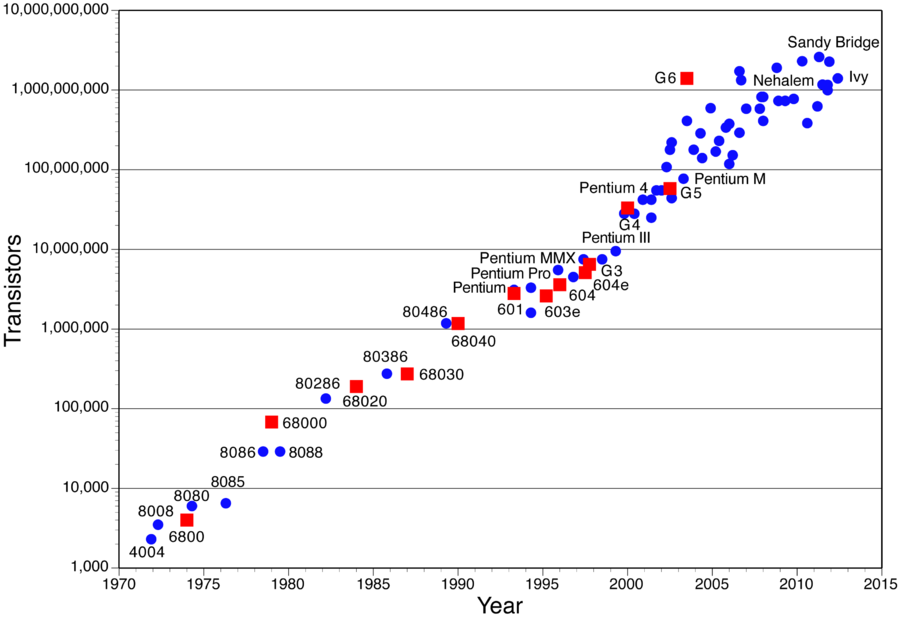
\includegraphics[width=.95\linewidth]{img/02/moorelaw.png} 
        \caption[Loi de Moore]{Nombre de transistor par processeur en fonction du temps ou loi de Moore}
 		\label{fig:moore}
\end{figure}

\begin{figure}[bth]
        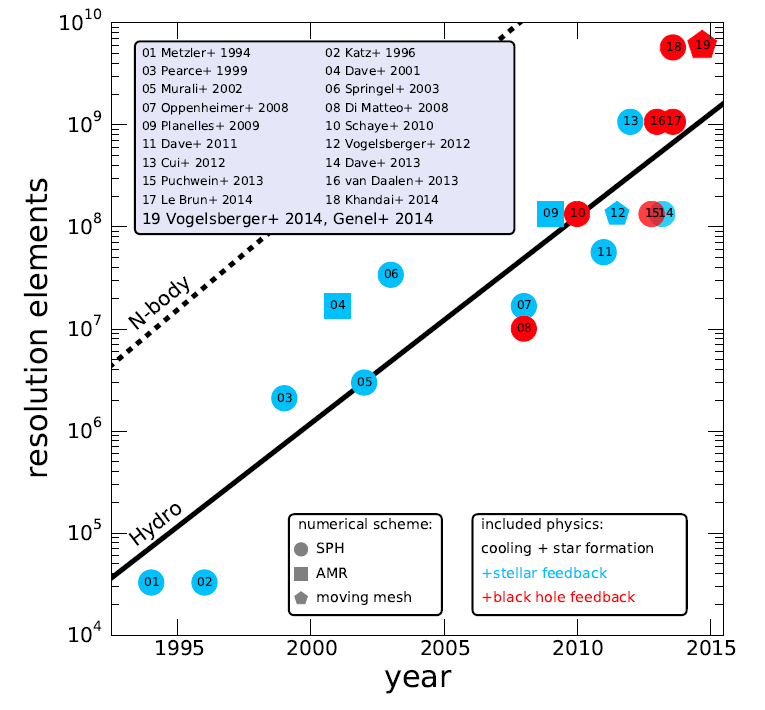
\includegraphics[width=.95\linewidth]{img/02/figure_simulations_with_time.png} 
        \caption[Évolution de la taille des simulations]{Tailles des simulations en fonction du temps.
        Il existe un lien direct avec la loi de Moore.
        Image illustris}
 		\label{fig:taillesimu}
\end{figure}


\subsection{Principes de parallélisation}

Comme on ne peux pas créer des processeurs aussi gros que ce que l'on le souhaite, la technique utilisée pour continuer à augmenter la puissance de calcul, consiste à en utiliser plusieurs en parallèle.
Dans le cas des simulation cosmologique, la parallélisation est effectué en découpant l'espace à simuler en un certain nombre de sous domaines chacun associé à une unité de calcul.
Comme chaque sous domaine n'est pas isolé, mais appartient au même ensemble, les domaines vont devoir communiquer entre eux sur l'état de leurs voisin.
Nous verrons en détail comment est effectué ce découpage dans la section \ref{sec:parasoft}.
Mais voyons d'abord un aperçut des contraintes techniques de la parallélisation.
Il existe différent type de parallélisation définis par la taxonomie de Flynn \citep{Flynn:1972:COE:1952456.1952459}: 

\begin{itemize}
\item SISD Single Instructions on Single Data.
Aucun parallélisme, exécution d'une unique série d'instructions sur un unique flux de données.

\item SIMD Single Instructions on Multiple Data.
Exécution d'une unique série d'instructions sur différents flux de données.
C'est le principe de fonctionnement des GPU.

\item MISD Multiple Instructions on Single Data 
Exécution de différentes série d'instructions sur un seul flux de données.

\item MIMD Multiple Instructions on Multiple Data.
Exécution de différentes série d'instructions sur différents flux de données.
C'est l’architecture la plus utilisée aujourd'hui, et celle qui nous intéresse ici.
Le type MIMD est lui même découpé en deux sous ensembles : 

\begin{itemize}
\item On dit que la mémoire est \textit{distribuée} quand les processus ont leurs propres espaces mémoires dédiés.
Les principales machines que j'ai pu rencontrer utilise un modèle MIMD à mémoire distribuée.

\item On dit que la mémoire est \textit{partagée} quand plusieurs processus ont accès au mème espace mémoire.
\end{itemize}
\end{itemize}

Il existe plusieurs niveau de parallélisation, au niveau matériel.
Par exemple, un processeur actuel dispose de plusieurs cœurs, capable de géré chacun un processus (voir 2 dans le cas de l'hyperthreading).
Il est possible d'avoir plusieurs processeur au sein d'un même ordinateur.
Et il est possible d'utiliser conjointement plusieurs ordinateurs.
Ce qui nous mène à la notion de centre de calcul.

\subsection{Les calculateurs}

La production de simulation cosmologique à haute valeur scientifique se fait sur des centres de calcul.
A la manière d'un télescope pour les observateurs, les supercalculateur sont les outils principaux des simulateurs.
Et a la manière des plus gros télescopes, ces calculateurs sont gigantesques.
La figure \ref{fig:titan} présente le calculateur TITAN du Oak Ridge Leadership Computing Facility sur lequel ont été exécutées les simulations CODA \citep{ocvirk_cosmic_2015}.
En novembre 2015, TITAN a été classé deuxième plus puissant calculateur au monde selon le cite top500.org (cf \ref{tab:top500}), il est aujourd'hui quatrième.

\begin{figure}[bth]
        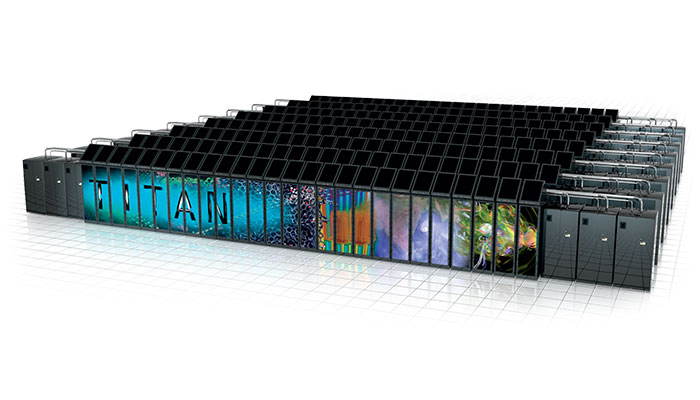
\includegraphics[width=.95\linewidth]{img/02/titan.jpg} 
        \caption[Titan]{Supercalculateur Titan OLCF.
        La calculateur sur lequel ont été exécutés les simulations CODA}
 		\label{fig:titan}
\end{figure}

\begin{table}[bth]
\begin{tabular}{ l l l l }
\hline 
Système & Pays & nb de cœurs & TFlop/s (peak) \\
\hline 
Sunway TaihuLight & Chine & 10,649,600 & 125,435.9 \\ 
Tianhe-2  & Chine & 3,120,000 & 54,902.4 \\ 
Piz Daint  & Suisse & 361,760 & 25,326.3 \\ 
Titan  & États unis & 560,640 & 27,112.5 \\ 
Sequoia  & États Unis &1,572,864 & 20,132.7 \\ 
\end{tabular} 
\caption[TOP500]{Les 5 super calculateurs les plus puissants du top500 de Juin 2017, source : www.top500.org}
\label{tab:top500}
\end{table}

Ce type de calculateur est composé d'un certain nombre de nœud qui communique entre eux par l'intermédiaire d'un réseau.
Un nœud est un élément conceptuellement proche d'un ordinateur personnel puisqu'il dispose d'une carte mère, avec un (ou plusieurs) \ac{CPU}, de la mémoire RAM, un \ac{SSD}/\ac{HDD} et parfois un \ac{GPU}.
D'une manière générale, plus des composants sont physiquement éloignés, plus leurs communications seront lente (cf \ref{tab:debits}).
La quantité d'information passant par une interface représente un certain coup et on cherchera à minimiser ce coup en optimisant le transfert des données à différents niveaux.

\begin{table}
\begin{tabular}{ l l }
\hline 
Interface  & Débit théorique \\
\hline 
Cache L1 & $\approx$ 700Go/s \\
RAM & $\approx$ 20 Go/s \\ 
PCIE 16x & $\approx$ 16 Go/s \\
InfiniBand & $\approx$ 5 Go/s \\
SSD & $\approx$ 600 Mo/s \\
HDD & $\approx$ 100 Mo/s
\end{tabular} 
\caption[Débits interfaces]{Ordre de grandeur des débits théorique des différentes interface rencontrées lors de l'exécution d'un code HPC.
On cherchera à optimiser les communications utilisant les interfaces les plus lentes.}
\label{tab:debits}
\end{table}

%Les cœurs au sein d'un même CPU pourront communiquer entre eux de faible quantité de données par l’intermédiaire du cache, ou en passant par la RAM pour les volumes plus importants.

%Proche d'un ordinateur personnel un nœud est composé d'une carte mère sur laquelle est relié entre autres, un ou plusieurs processeurs (CPU), une certaine quantité de mémoire RAM et parfois une carte graphique (GPU)
%Chaque CPU dispose d'un certain nombre de cœurs, et chaque cœurs est capable d'exécuter un certain nombre de processus ou thread (généralement 1, parfois 2 dans le cas de l'Hyperthreading)

%Une fois les processus et les domaines identifiés il existe différentes facons de faire dialoguer les processus entre eux.
%La principale distinction viendra généralement de si les threads sont exécutés par un meme noeud ou non.
%
%, cad par exemple que si le thread 0 déclare une variable X, le thread 1 aura aussi accès a cette variable . 
%OpenMP est une API permettant ce  genre partage de mémoire.

%Si les threads sont exécutés sur un même nœud on aura tendance a utiliser un schéma a base de mémoire partagée.
%
%Dans le cas ou les threads sont exécutés par des processeurs étant physiquement éloigné, ie sur des noeuds différents, les communications doivent passer par un réseau de communication reliant les noeuds.
%Il faudra utiliser dans ce cas une autre API pour explicitement envoyer et recevoir des paquets d'information
%L'API la plus communément utilisée pour ce genre de communication est Message Passing Interface MPI.
%
%\paragraph{Nœud :} Élément du centre de calcul relier par un réseau.
%
%La difficulté est de géré la façon dont les threads travaillent ensemble.
%En effet a chaque thread sera associé un domaine de calcul représentant une partie de l'espace a modéliser.
%De plus les domaine ne sont pas isolés et partage de l'information. 
%
%Nous sommes alors confronté a plusieurs problèmes: comment associer les threads aux domaines de calculs  et comment faire communiquer ces threads entre eux.
%
%Ces machines se composent d'un certain nombre de nœuds.

Généralement, la mémoire est partagée au sein d'un nœud, et distribuée sur le réseau.
C'est a dire que tout les processus au sein d'un même nœud pourront communiquer par l'intermédiaire de la RAM, ce type de communications est rapide.
Pour les communications entre les nœuds, l'information devra passer par le réseau, ce type de communications est donc plus lent.
Et ce d'autant plus que les nœuds sont physiquement éloignés entre eux.

\subsection{Courbe de Peano-Hilbert}
\label{sec:parasoft}

%https://books.google.fr/books?id=sbQqBgAAQBAJ&pg=PA26&lpg=PA26&dq=peano+hilbert+mpi&source=bl&ots=HgSw0Jpf7d&sig=vXTb2JkDixd1gcDGANoARIYHAG0&hl=fr&sa=X&ved=0ahUKEwilofzKoerSAhUF6RQKHXzQDC4Q6AEIGjAA#v=onepage&q=peano%20hilbert%20mpi&f=false


%Durant le développement d'un code HPC, on cherchera a minimiser les communications
%, et plus spécifiquement celle par le réseau qui sont nombreuse et relativement lentes.
%Warren et Salmon
Dans le but de garder une certaine proximité spatiale, le découpage des domaines de calcul correspondants aux différents processeurs, utilise une courbe de Peano-Hilbert.
Ce type de courbes fractale a la particularité de remplir l'espace et de passer par tout les points d'une grille.
Ainsi si l'on applique ce pavage aux cellules de notre grille, en associant un indice reliant une cellule à sa position sur la courbe de Hilbert.
Il suffit ensuite de découper la courbe en parties identique pour définir quelles cellules seront associées à quels processus.
Ainsi si l'on a par exemple 32 cellules à assigner sur 4 processeurs, la courbes sera découpée en 4 parties de 8 cellules.
Chacune de ces parties sera en suite assignée à un processeur.
Ce type de découpage minimise les interfaces entre domaine, en s'assurant d'une proximité spatiale entre tout les points de la courbe.

\begin{figure}[bth]
        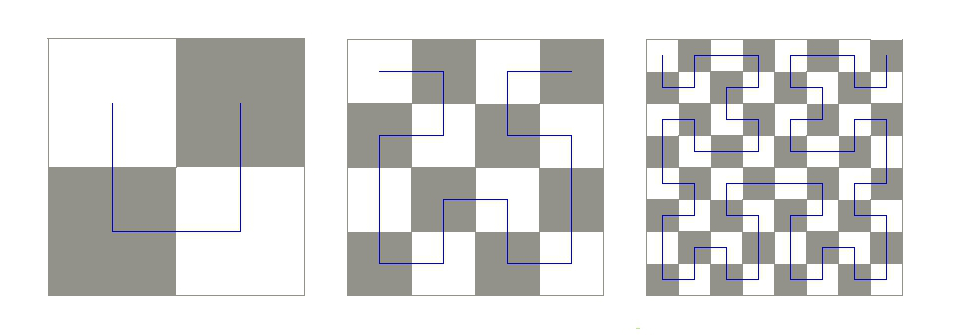
\includegraphics[width=.95\linewidth]{img/02/courbe_Hilbert.jpeg} 
        \caption[Courbe de Hilbert]{Principe de la courbe de Hilbert. 
        %http://www.lifl.fr/~pmathieu/transform/fractales.html
 		\label{fig:hilbert}}
\end{figure}

%
%\begin{figure}[bth]
%        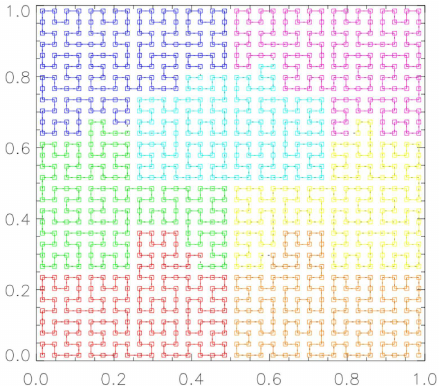
\includegraphics[width=.95\linewidth]{img/02/hilbert2.png} 
%        \caption{exemple de courbe de Hilbert. 
%%http://iopscience.iop.org/article/10.1086/590370/pdf 
%}
% 		\label{fig:hilbert2}
%\end{figure}

Dans l'état actuel de EMMA, la courbe est calculée au début de la simulation, et seule la grille coarse est prise en compte.
La répartition des domaines est statique et n'évolue pas au cours de la simulation.
Dans le cas ou un domaine raffine plus qu'un autre, la charge de travail y est plus importante.
Dans le futur, l'objectif serait de calculer la courbe de Hilbert sur la totalité des cellules feuilles.
Pour ainsi pouvoir refaire le découpage et équilibrer la charge entre les processeurs, et réaliser un "load balancing".

\subsection{Les domaines}

Chaque processus dispose d'un domaine de calcul correspondant à une sous partie de la grille.
Cependant, les domaines doivent communiquer entre eux et doivent être sensible a la structure \ac{AMR} de leurs voisins.
Pour répondre à ce problème, EMMA utilise le "Local essential tree decomposition" \citep{Warren:1993:PHO:169627.169640}.
Chaque processus dispose d'une vue globale de toute la grille ( cf Fig. \ref{fig:domaine}) mais la partie de la grille qui n'appartient pas au processeur est vue a résolution dégradée.
Ceci facilite grandement le gestion des conditions de bords.

\begin{figure}[bth]
        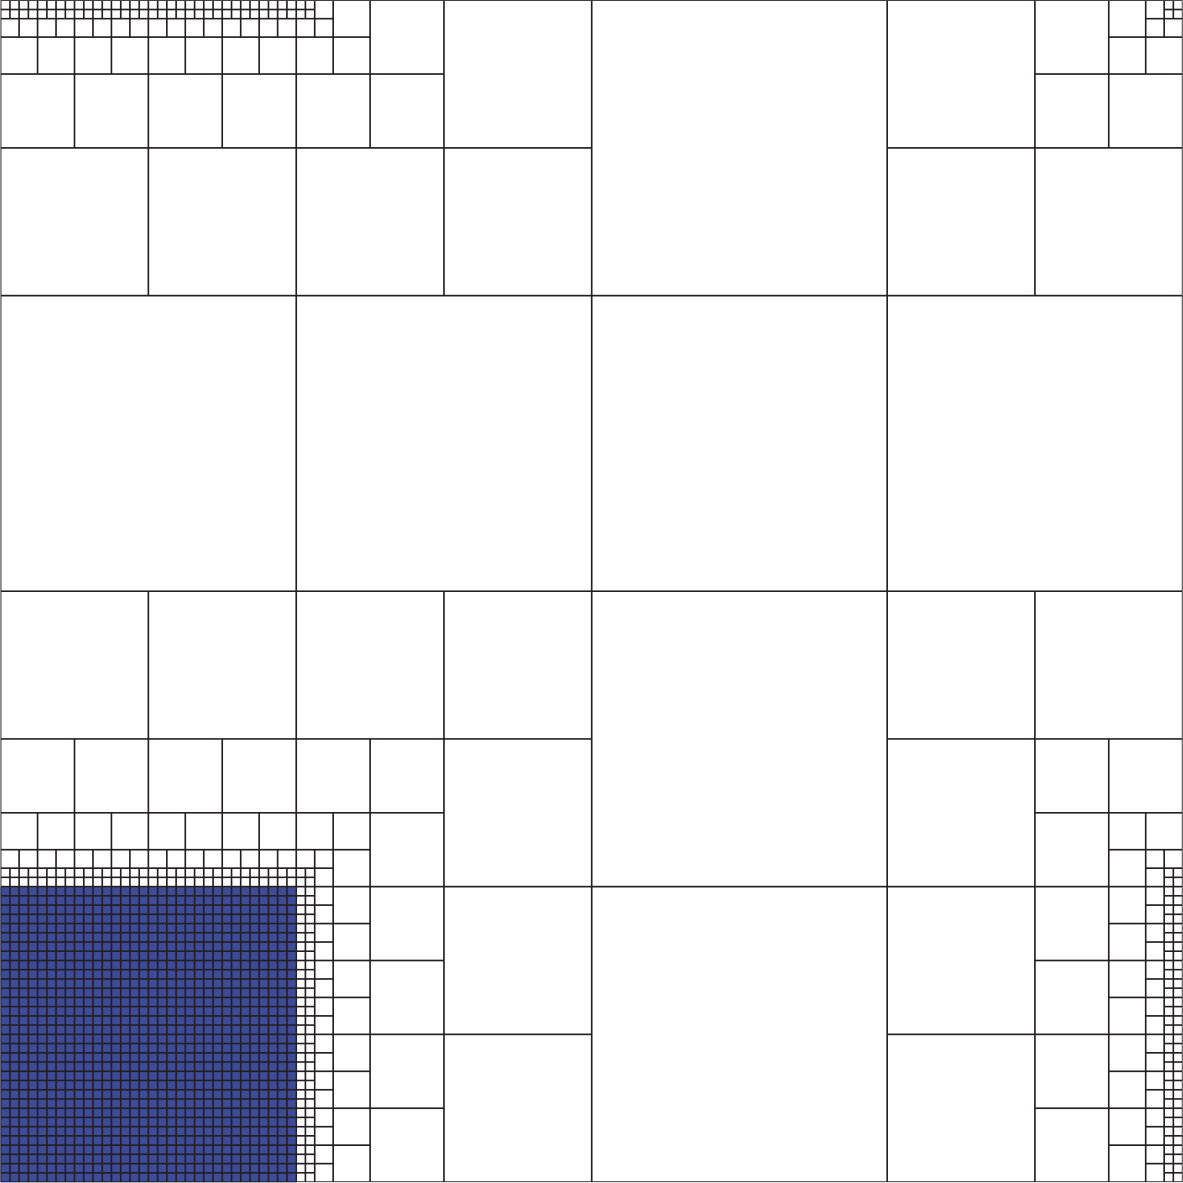
\includegraphics[width=.95\linewidth]{img/02/secteur.png} 
        \caption[Domaine associé a un processus]{Exemple de domaine de processeur généré par EMMA. 
        Chaque domaine représente une vue d'ensemble de la grille, a résolution dégradée.
}
 		\label{fig:domaine}
\end{figure}

\subsection{GPU}

EMMA utilise un degré supplémentaire de parallélisation.
Les calculs de chaque domaines sont accéléré en utilisant les capacités parallèle des processeurs graphiques récents.
Les cartes graphiques, ou \ac{GPU} ont été détourné de leurs utilisation principale d'affichage il y a une dizaine d'années et offre une capacité de parallélisation importante. 

A l'inverse des \ac{CPU} actuels qui disposent d'un nombre réduit de cœurs, les \ac{GPU} disposent d'une nombre beaucoup plus important de cœurs.
Par exemple un AMD Opteron 6300 de TITAN dispose de 16 cœurs, contre 2880 cœurs pour une NVIDIA Tesla k40c.
Un  \ac{CPU} peux exécuter des taches différentes sur chacun de ses cœurs (MIMD) tandis ce que les \ac{GPU} utilise un mode de parallélisation de type SIMD (Fig \ref{fig:cpugpu}).
Ce mode de parallélisation en font des unités de calculs efficaces dans le traitement d'un grand nombre d'informations en parallèle.
Elle sont donc toutes indiqués dans le cas des simulations numérique ou il s'agit d'appliquer un traitement identique à un grand nombre de cellules.

\begin{figure}[bth]
        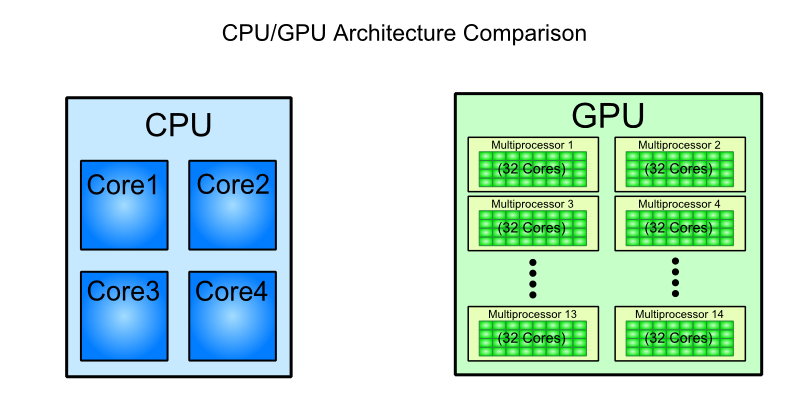
\includegraphics[width=.95\linewidth]{img/02/cpu_vs_gpu.png} 
        \caption[Comparaison CPU/GPU]{Comparaison CPU/GPU. Un \ac{CPU} dispose d'un nombre réduit de cœurs capables d’exécuter des opération complexe. 
        A l'inverse un \ac{GPU} dispose d'un grand nombre de cœurs pouvant exécuter un grand nombre d'opérations simples en parallèle}
 		\label{fig:cpugpu}
\end{figure} 

De plus, il existe au niveau matériel, deux avantages des \ac{GPU} par rapport aux \ac{CPU}.
Premièrement leurs meilleurs ratio puissance de calcul sur coup (flop/€).
Et également un meilleur ratio puissance de calcul sur puissance électrique (flop/W) ce qui réduit les besoins de refroidissement et permet des économies supplémentaires.

Cependant \ac{CPU} et \ac{GPU} sont indissociables est doivent être utilisé conjointement pour tirer le meilleurs parti des capacités de calcul offerte par une machine hybride.
La programmation sur carte graphique utilise une approche proche du concept de mémoire distribuée, c'est à dire que leurs espaces mémoire ne sont pas commun.
Une code hybride est découpé en deux parties, une partie séquentielle exécutée sur le \ac{CPU} et une partie parallèle exécutée sur le \ac{GPU}.
Le passage de \ac{CPU} à \ac{GPU} va donc nécessiter des communications.

%On tirera le maximum des capacités d'accélération d'un \ac{GPU} avec un code qui est hautement parallélisable.

%Il faut donc que la quantité de calcul effectués par la carte soit suffisante pour rentabilisé la communication.
%plus dur a programmer, performance dépends du problème.


%Or a l'heure actuelle cette communication utilise une interface relativement lente (PCI express) qui rend coûteuse la communication. 

% et de 12Go de mémoire et a une puissance de calcul de 4.3 Tflop/s en simple precision.
%
%
%Intel® Xeon® X7560 -> TDP 130 W -> 76 Gflop/s (crete)
%
%
%IBM A2 (sequoia) -> 204 Gflop/s -> TDP 55W


\subsection{Les communications CPU/GPU}
\label{sec:cpugpu}

Les \ac{CPU} sont capable d'accéder rapidement aux informations en mémoire, quel que soient leurs organisations.
Le \ac{GPU} sont quant à eux sensibles à la segmentation des données.
C'est à dire que les calculs sur ac{GPU} seront plus performants si les données sont organisées de façons à ce que leurs accès mémoire consécutifs soient physiquement proches.
%Prenons l'exemple d'une différence finie. 
%Pour calculer le nouvel état d'une cellule, il est nécessaire de connaitre sont état actuel, et celui de sa voisine.
%L'accès mémoire sera plus rapide si l'information est situer sur un espace mémoire adjacent.
%Ce choix est motivé par le fait qu'une structure mémoire bien organisée peux amener a des gains conséquents.
Par exemple dans CUDATON \citep{aubert_radiative_2008} un code de transfert radiatif sur grille fixe, le gain de la parallélisation GPU est de l'ordre de 80 car la structure mémoire est optimisée.

La difficulté est que l'arbre \ac{AMR} ne respecte pas cette organisation, et la mémoire peut être extrêmement fragmentée à cause de la liste chainée.
Pour limiter l'impact de la fragmentation, le choix a été fait d'organiser les données sur le CPU, avant de les envoyer dans l'espace mémoire du GPU.
Cette opération sera appelée "gather" (cf Fig. \ref{fig:gatherscatter}).
Les données organisées sont envoyés sur le GPU, pour effectuer les calculs.
Le résultat est ensuite copié sur le CPU et remises dans l'arbre par le CPU (opération de "scatter").
Dans le cas où les calculs sont réalisés sur le CPU, cette opération est quand même réalisée, dans le but de conserver une certaine cohérence entre les versions.

\begin{figure}[bth]
        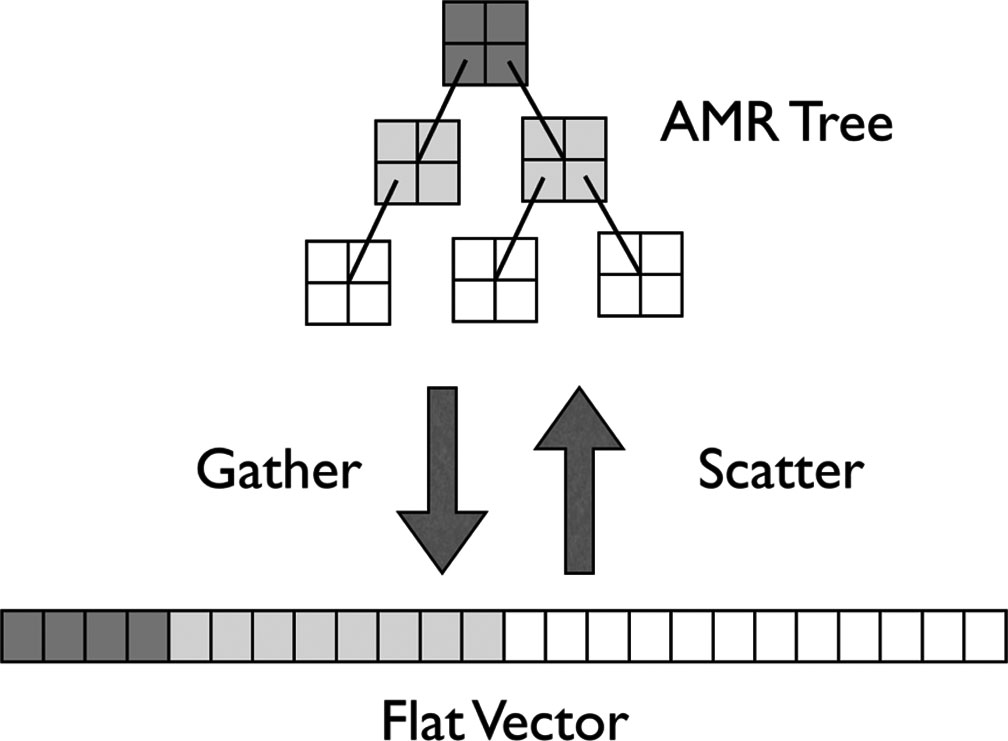
\includegraphics[width=.95\linewidth]{img/02/gatherscatter.jpg} 
        \caption[Passage AMR / vecteur]{Transition entre la structure en arbre de l'AMR et la structure en vecteur de calcul.
        L'arbre est sur le CPU, le vecteur est sur le GPU.
 		\label{fig:gatherscatter}
 		}
\end{figure}

Le pari est ici que la perte de temps générée par les opérations de gather/scatter sera compensé par l'accélération du GPU.

En pratique l'opération de gather consiste a rassembler toutes les informations nécessaire au calcul de l'état d'une cellule.
Par exemple pour le calcul du potentiel (cf sec. \ref{sec:gravity}) les données nécessaires seront: la densité locale, le potentiel local, le potentiel des 6 cellules voisines suivant les axes principaux.
Ces données sont rassemblées dans une structure, puis une série de structure est stockée dans un tableau.
Cette opération sera réalisée par paquet de $N$ cellules pour chaque cellule de la grille.

On peut observer ici que les copies ont beaucoup de redondance.
la copie est composé d'une cellule centrale et des 6 cellules voisine le ratio information utile sur information nécessaire est de $1/6$..
En passant à la cellule suivante, la cellule précédente sera de nouveau copiée et au final le potentiel d'une cellule sera donc copié sept fois sur le GPU.
Ces multiples copies diminue grandement les performances et en font l'une des principales limitations à l'accélération globale du code.
Toute fois, même dans cet état, l'exécution s'en trouve accélérée d'un facteur $\approx 3$ par rapport à la version CPU.

Dans le but de réduire le nombre de copies et accélérer l'exécution du code, j'ai modifié les opérations de gather/scatter pour diminuer la redondance des copies.
Au lieu de traiter les cellules unes par unes, l'idée est de traiter les octs.
Dans ce cas les cellules sont traitées par 8 et les voisinages au sein d'un oct n'ont pas besoin d'être copiés plusieurs fois.
On copie donc 8 cellules d'intérêt et 4 cellules de bord par face du cube, soit 24 cellules.
Le ratio utile/nécessaire passe donc à $8/24 = 1/3$.
La quantité de copies redondante a donc été divisé par 2 par rapport au cas précédent.

Vu que la surface d'un cube augmente avec le carré de son coté, alors que son volume augmente avec son cube, plus grand sera la nombre de cellule d'intérêt, meilleur sera la ratio.
En étendant ce principe, j'ai développé une méthode qui permet de manière récursive d'envoyer une portion d'AMR contenue dans un OCT de niveau arbitraire.
Cependant les résultats ne sont pas a la hauteur des espérances, et l'accélération n'est pas proportionnelle au ratio de données utiles.

IL existe cependant des pistes pour améliorer ce goulot d'étranglement.
Une possibilité est de séparer la gestion de l'arbre de la physique.
En l'état actuel, les données physique sont stockées en mémoire avec la même structure que l'arbre.
L'idée serait de stocker dans l'arbre, des indices de cellules permettant de retrouver l'information physique dans des vecteurs plat (cf Fig. \ref{fig:gatherscatter}).
Ainsi les vecteurs pourraient être en permanence sur le GPU, et seul l'information sur leurs position dans l'AMR devrait être transmise.
Un grand nombre de copies seraient alors évitées. 

Une autre possibilité serait de placer l'intégralité de l'arbre sur le GPU.
Dans ce cas, toutes les copies seraient supprimées mais c'est le GPU qui devra gérer l'évolution de l'arbre. 
Il existe des techniques optimisé de gestion d'arbre sur GPU à base de "Z-order curves", mais son implémentation nécessite une refonte en profondeur du code.

%optimisation matérielle -> les prochaines générations de GPU


%est de séparer la gestion de l'arbre de la physique.
%La plus prometteuse semble être de supprimer complètement les copies en plaçant la totalité de l'arbre directement sur la carte.
%Le CPU étant tres efficace pour ce genre d'opération, il semble

%Copies asynchrones

\subsection{Gestion des entrées sortie}

Durant ma thèse la simulation CODA II EMMA (voir partie \ref{sec:CODAEMMA}) a été réalisée.
Cette simulation fait partie des plus grosse simulation de la réionisation exécutée à l'heure actuelle avec un nombre de particules de matière noire, et donc une grille de base, de $2048^3$ éléments .
Ces données devront être stockées et écrites sur disque dur or si l'on se réfère à la table \ref{tab:debits} on observe que les débits d'accès disques sont les plus faibles.

Pour se faire une idée de la quantité de données en jeu faisons une estimation : 

\begin{itemize}
\item Pour les particules:
En considérant qu'un flottant est codé sur 4 octets, chaque champs représente $2048^3 \cdot 4 = 32$Go.
Comme il y a une dizaine de champs en sortie (3 positions, 3 vitesses, etc) les particules représentes environs $320$Go.

\item Pour la grille :
En considérant que la quantité de cellule peut être multipliée par 3 à cause du raffinement, chaque champ (densité, température, composante de la vitesse, etc..) représente environ $32 \cdot 3 \approx 100$Go.
Il y a au total un cinquantaine de champs calculés à l'exécution de la simulation mais en pratique environ une vingtaine en sortie.
Chaque écriture de la grille représente donc $100\cdot 20 =2$To.

\item Pour les étoiles:
C'est très variable car dépend directement du nombre d'étoile à l'instant donné, qui dépend lui même du paramètre de résolution en masse.
\end{itemize}

Ce qui représente au total environ 2,3 To de données générée par pas de temps de sortie.
Mais on voudrait évidemment avoir accès a l'état de la simulation à différents instant, cette simulation a au final générée 170 snapshot.
Au final le volume de donnée de la simulation représente près de 400 To.
%De plus, ces données sont stockées sur \ac{HDD}, et si l'on se réfère à la table \ref{tab:debits} on observe que les débits d'accès disques sont les plus faibles.
Étant donné la quantité de données en jeu, une bonne gestion des Entrées/Sorties peut donc permettre un gain de temps appréciable.
De plus, ces données sont généralement calculé sur des machines distante et améliorer leur compacité peut permettre de gagner du temps au moment du transfert vers des machines locales, ou simplement au moment de la lecture pour analyse.

%Les entrées/sorties sont des étapes relativement longues et l'écriture sur disque d'une telle quantité de données demande du temps et ralentit l'exécution de la simulation.
% leurs rapatriement sur des machine locales peut également être coûteux en temps.
%Il a fallu plusieurs mois pour rapatrier localement les données générées par la simulation CODA.
%Il a fallut plusieurs mois pour rapatrier les données de CODA de TITAN aux états unis vers Strasbourg
%De plus améliorer la compacité des données permet également de gagner du temps au moment du transfert vers des machines distante, ou simplement au moment de la lecture
%analyse a distance
%le feedback CODA\\
%grosse quantité de données\\

Dans l'ancien modèle de données d'EMMA, l'intégralité de l'octree était écrit (cf figure \ref{fig:data}).
Les octs étaient écrit les uns à la suite des autres avec toute l'information qu'ils contenaient.
L'information étaient exacte et complète, mais le volume de données était considérable.
De plus chaque processeur écrivait un fichier indépendant, ce qui pouvait rapidement faire exploser le nombre de fichiers et être problématique selon file-système des calculateurs car il est possible d'avoir un nombre limité de fichier par utilisateur.

Dans la même optique que ce qui a été abordé dans la section \ref{sec:cpugpu}, j'ai mis en place un modèle visant a manipuler les données avant leurs transferts.
L'objectif est de sortir les données de l'arbre en se basant sur une notion de tableau de champs pour faciliter leurs traitement.
Dans ce nouveau modèle, seules les feuilles (les cellules non raffinées) sont écrites sur le disque, ce qui permet de réduire le volume et la redondance des données.

Les champs sont maintenant traités individuellement (cf figure \ref{fig:data}) et il est possible de choisir de les écrire ou non en fonction des besoins.
Les champs sont séparés dans des fichiers distincts, et les processeurs écrivent conjointement dans le même fichier grâce a l'utilisation de la librairie hdf5.
Le nombre total de fichiers ne dépend plus du nombre de processeurs sur lequel a tourné la simulation.
Et lors d'un transfert entre machine, il est possible de ne rapatrier que les données nécessaire, et ainsi économiser du temps et de la bande passante.

Malgré la quantité de données réduite, le temps passé dans la fonction de sortie n'en est que très peu affecté.
Le gain réalisé au moment de l'écriture est compensé par la charge de calculs supplémentaires due à l'extraction des données de l'arbre.
Par contre un gain appréciable est réalisé au moment de l'analyse des données.

\begin{figure}
        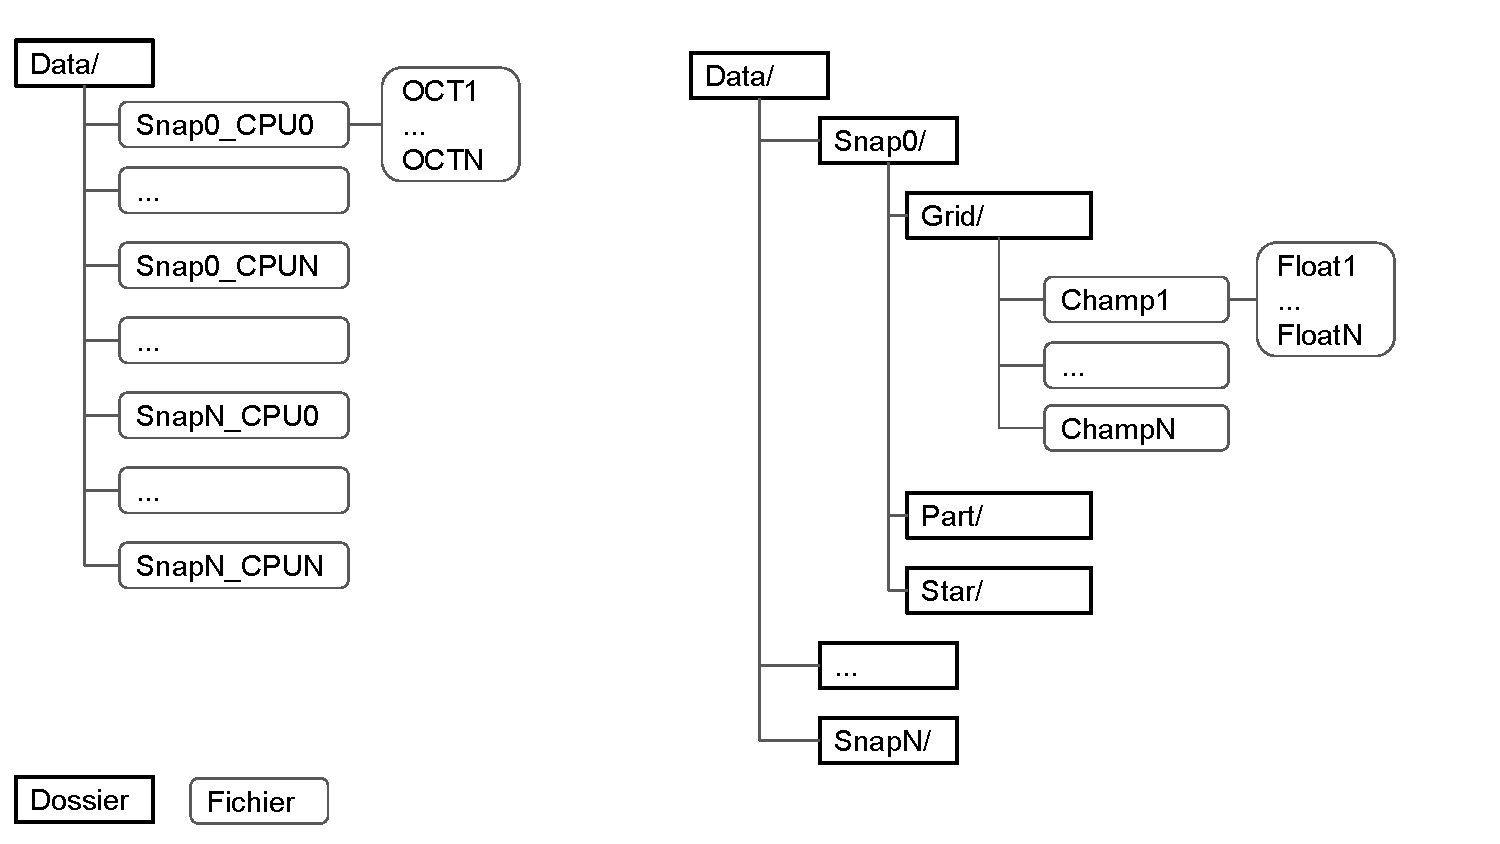
\includegraphics[width=.95\linewidth]{img/02/data.pdf} 
        \caption[Gestion des IO]{Différence entre ancienne gestion des données à gauche et nouvelle version à droite.
 		\label{fig:data}
 		}
\end{figure}


%En contrepartie, il est nécessaire de reprojeter la grille dans le cas d'une analyse sur un niveau intermédiaire.

%Chaque cellule est considérée comme une particule d'une certaine taille.

%Architecture des données 
%conception d'une organisation des données
%séparation des champs
%structure imposé par la gestion de l'AMR
%écriture parallèle

%\subsection{Potentiel d'optimisation EMMA}
%
%la forme des gathers/scatter
%optimisation matérielle -> les prochaines générations de GPU
%Opérations coarse sur grille non AMR.
%reformatage de l'arbre et découplage de la physique


%\begin{figure}[bth]
%        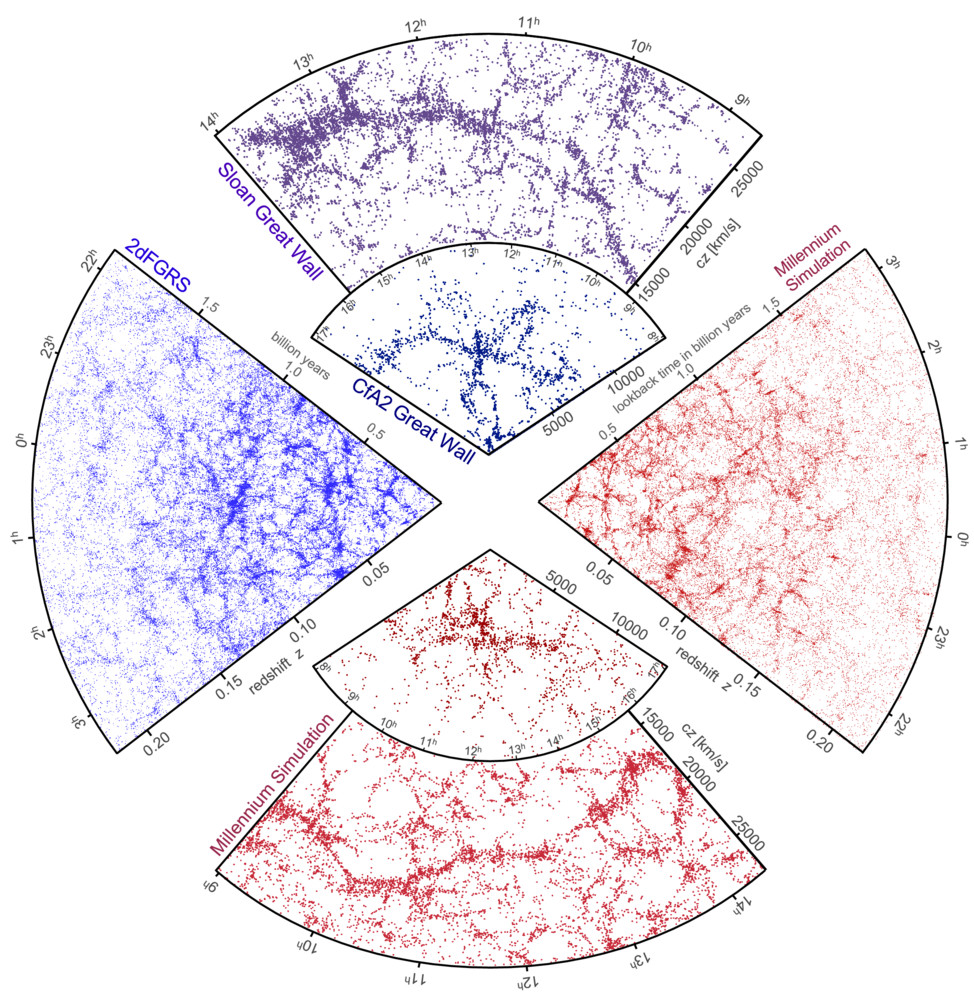
\includegraphics[width=.95\linewidth]{img/02/sdss_millenium.jpeg} 
%        \caption{ 
%%http://wwwmpa.mpa-garching.mpg.de/millennium/
%}
% 		\label{fig:}
%\end{figure}


%
%\cleardoublepage
%\ctparttext{Cette partie est liée a la publication présentée en annexe\,\ref{pap:feedback}.\medskip
%
%\emph{"Radiation and supernovae feedback during the epoch of reionization with EMMA"} \medskip
%
%Nicolas Deparis, Dominique Aubert, Pierre Ocvirk et Nicolas Gillet.
%Soumis à MNRAS.
%
%\vspace{1cm}
%Ainsi qu'au proceeding de conférence présenté en annexe\,\ref{pap:feedback_proceeding}.\medskip
%
%\emph{"Stellar feedback during the reionization with EMMA"} \medskip
%
%Nicolas Deparis.
%SF2A-2016.
%
%}
%\part{La composante stellaire}
%
%%\addtocontents{toc}{\protect\clearpage} % <--- just debug stuff, ignore
%\chapter{Les étoiles}


Maintenant que nous avons survolé toutes les physiques a l’œuvre dans ce type de simulation, concentrons nous sur les sources lumineuse.
comme nous avons vu, il existe deux types de sources, les étoiles et les quasars. %TODO ref
Je n'ai considérer que la partie stellaire.

L'objectif de cette section est d'exposer le modelé stellaire que j'ai développé.
Nous allons définir les différentes phase de la vie d'une étoile, et ses différentes évolution possible.
Nous verrons qu'elles sont les contraintes imposées par la résolution des simulations cosmologique.



\section{Les différentes phases de la vie d'une étoile}

Nous allons nous intéresser dan cette partie aux différentes phases de la vie d'une étoile.
Nous allons aborder la naissance, la vie et la mort d'une étoiles de manière générale dans un premier temps.
Et nous verrons dans un second temps l'implémentation de ces trois phases dans EMMA 

\subsection{Naissance}

%lien avec la densité\\
%Formation dans l'H moléculaire mais pas dans les simu

En principe une étoile se forme par effondrement gravitationnel.
Dans un nuage, si le temps de chute libre est supérieur au temps de rection a une perturbation le milieu n'a pas le temps de résister a son effondrement et le gaz s'effondre sur lui même.
Cette ne s'arrête que quand les réactions thermonucléaire s'enclenche et que le gaz forme une étoile.

Il y a effondrement si:
\begin{equation}
t_{ff} < t_{sound},
\end{equation}

avec:
 
\begin{equation}
t_{ff} = \frac{1}{\sqrt{G \rho}},
\end{equation}
et
\begin{equation}
t_{sound} = \frac{R}{C_s},
\end{equation}

Ici intervient la densité, plus le milieu est dense plus il aura tendance a s'effondrer sur lui même.
D'un autre coté intervient aussi la vitesse du son $C_s$, elle même dépendante de la température $C_s \propto \sqrt{T}$.
Plus le gaz sera chaud, plus le nuage devra être gros pour pouvoir s’effondrer.

\subsection{Population III}

%tres peu de ligne de refroisdissment
%étoiles plus grosse
% temps de vie court

Or a haut redshift, au moment de l'apparition des premières étoiles, les métaux étaient très peux disponible  (voir :\ref{sec:nucleosynthese_primordiale})
De ce fait, le gaz disposait de relativement peu de possibilité de refroidissement, et donc la température du gaz devait être élevée.
Les étoiles primordiales devaient donc être plus grosses que les étoiles de notre voisinage (plus de 100Mo).
Ce type d'étoiles est appelées étoiles de population III.
Du fait de leur masse, elles émettait un fort rayonnement ionisant, et avaient une vie relativement courte.



%La nucléosynthèse primordiale a créer peu de métaux. 
%A haut redshift, les metaux etaient peu disponible.
%les métaux permettent une meilleur emmission radiative, et donc un meilleur refroidissent.
%si le refroidissment est meilleur, l'equilibre hydrostatique penche an faveur de plus grosse étoiles.
%POPIII, IMF top Heavy, étoiles  primordiales
%
%plus un étoiles est grosse, plus son spectre sera énergétique et plus la portion de spectre ionisant sera important.



\subsection{Séquence principale}

%le diagram HR


Une fois le nuage de gaz effondré et les réaction thermonucléaire amorcées.
l'étoiles amorce sa séquence principale.
C'est la phase qui représente la majore partie de la vie d'une étoile.
Elle consiste en un équilibre hydrostatique entre gravitation et réaction de fusion nucléaire nucléaire.

%develloper le cycle proton proton ?
Équation simplifié du processus de fusion:
\begin{equation}
4p \leftrightarrow He^4 + 2e+ + 2\nu + E
\end{equation}

L'étoile va donc consommer son hydrogène pour résister a l'effondrement gravitationnel.
Il en résultera la formation d'hélium.

Plus une étoile est grosse plus le taux de réaction doit être élevé pour lutter contre la gravité.
Il en résulte que les grosse étoiles sont plus énergétique, et emmetent donc plus de rayonnement ionisant.
Mais ce taux de réaction élevé mène a une durée de vie plus courte.

%materiaux de base est l'hydrogene\\
%plasma donc hydrogène ionisé 

\subsection{Mort}

Arrivé a un certain taux de consommation d'hydrogène, les réactions PP ne sont plus suffisante et l'étoile s'effondre sur elle même.
A la fin de sa vie, une étoile a consommée la plus grande partie de son hydrogène disponible.

L'équilibre entre la gravité et la pression radiative est rompu et l'étoile s'effondre, ce qui mene a une augmentation de la pression interne.
Cette augmentation de la pression amorce une nouvelle série de fusion nucléaire, qui va consommer des élément plus lourd que l’hydrogène.
C'est le début du cycle CNO.
Une fois arrivé au Fe, il devient coûteux de continuer a fusionner des éléments car Fe est le plus stable.

% Géante rouge ?

Il existe principalement deux types de supernovae : 
\begin{itemize}
\item les types I sont des étoiles binaire accrétante du compagnon -> passage au dessus de la limite.
\item les types II, l'étoile est assez massive des le départ (M>8Mo) Les étoiles de plus de 8Mo vont exploser en supernovæ et injecter 10 51 erg d'énergie dans le milieu.
\end{itemize}





formation d'éléments lourd (>Fe)
enrichissement du milieu

Après l'explosion de la supernova, le cœur subsiste et en fonction de sa masse, plusieurs scénario d'évolution sont possibles:
\begin{itemize}
\item Naine blanche (pression de dégénérescence des électrons)
\item Étoile a neutron (pression de dégénérescence des neutrons)
\item Trou noir (singularité)
\end{itemize}

Dans tout les cas, le résidu continue a interagir gravitationnellement.

\section{Population stellaire et modèle sous grille}

\subsection{Problème de résolution}

%En fonction des echelles de travail, nous considererons soit les etoiles individuelles soit une population stellaire.


Une des difficulté des modèles stellaire dans les simulations de réionisation, et le manque de résolution.
Il existe toujours ce conflit en réionisation entre simuler des grands volume, et obtenir la meilleur résolution possible.
Actuellement les simulations les plus résolues et capable de suivre un volume d'Univers suffisant atteigne un résolution de l'ordre de la centaine de parsec.
Or les échelles de formation stellaire sont de l'ordre de l'unité astronomique, soit un facteur $\approx 10^6$ plus petit.
Il n'est donc actuellement pas possible de suivre la formation des étoiles individuellement.

Il nous faut créer un modèle qui va tenter de prendre en compte au mieux la physique non résolue.
Ce type de modèle est appelé modèle sous grille.

Dans le cas présent le modèle sous grille consiste a transformer une partie du gaz en particule stellaire.
On appelle ces particules des particules puits.
Toute la difficulté du modèle de formation stellaire sera de déterminer la façon dont est réalisée cette conversion.
Malgré tout, nous verrons qu'il est possible d'obtenir un modèle statistiquement viable a grandes échelles assez facilement.

Un second type de modèle intervient au moment de l'explosion en supernovae.
Les processus de diffusion de l'énergie libérée aux échelles plus petite que la grille sont complexe et il en résulte une série de paramètres libres assez conséquente.

%lien entre les différents solveurs en fonction du stade évolutif
Les étoiles se trouvent aux centre de la simulation.
En effet, créer une étoiles consiste a transformer une partie du gaz en particule.
Cette particule sera ensuite gérée par le solveur Ncorps, et servira de source au solveur radiatif.
Puis a la fin de sa vie, l'étoile va injecter de l'énergie dans le solveur hydrodynamique.
Une particule stellaire va donc devoir interagir avec tout les solveurs du code.




%Seul la partie du spectre capable de ioniser l'hydrogène est considérée. E>13.6eV



\subsection{Fonction de masse Initiale}

Les étoiles naissent en groupe.
La probabilité de former une étoile d'une certaine masse est régie par la fonction de masse initiale (IMF)
Il existe différentes \ac{IMF}, parmi les plus connues il y a :

\begin{itemize}
\item \cite{1955ApJ...121..161S}
\item \cite{1979ApJS...41..513M}
\item \cite{2001MNRAS.322..231K}
\item \cite{2003PASP..115..763C}
\end{itemize}

Comme nous l'avons abordé plus haut, les étoiles de population III avaient tendance a être très massive.
De plus, certain travaux (eg \cite{2003MNRAS.344L...7C} ) suggère une \ac{IMF} top heavy, c'est a dire une \ac{IMF} avec une proportion d'étoile massive très importante.
La majorité des simulations que j'ai réalisées utilisent une \ac{IMF} Top-Heavy.

J'ai commencé mes calibrations avec une \ac{IMF} de Salpeter, mais il s'est vite avéré que les sources n’émettaient pas assez de photons et que les boites n'arrivaient pas a reioniser
%: difficulté a reioniser avec Salpeter -> passage a top heavy -> justification 
%Fonction de masse IMF Top Heavy


\subsection{Starburst99}

%Pour modeliser 
%paramètre d'entrée
%sorties

La modélisation de population stellaire est complexe, et il existe différent modèles complets.
J'ai choisi d'utilisé Starburst99 \citep{leitherer_starburst99:_1999} mais il en existe d'autres : \cite{2003MNRAS.344.1000B} , FSPS \cite{2009ApJ...699..486C}.  
%TODO mettre les differnts models

A partir d'information caractéristique d'une population stellaire, comme sa masse, son \ac{IMF} ou sa métallicité, Starburst99 retourne le spectre d'émission de cette population en fonction du temps cf (Fig \ref{fig:spectre_starburst}).

\begin{figure}[htbp]
        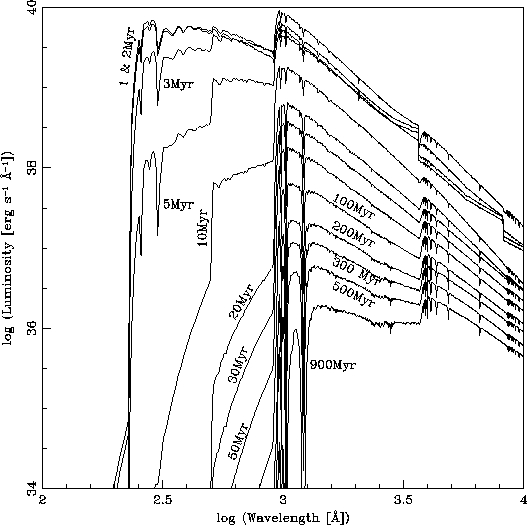
\includegraphics[width=.95\linewidth]{img/03/spectre_starburst.jpg} 
        \caption{Spectre d'émission d'une population stellaire généré par Starburst99.
        Ici avec les paramètres M=1e6 Mo, IMF de Salpeter ($\alpha=2.35$ et intégration de 1 a 100 M$_\odot$ }
 		\label{fig:spectre_starburst}
\end{figure}

Un avantage de Starburst99 par rapport a d'autre modèle et qu'il retourne également de l'information utile pour la modélisation des supernovae.
Nous y reviendrons dans la section dédiée. %TODO ref






\section{La formation stellaire}

\subsection{Localisation des zones de formation stellaire}

Il est admis que les étoiles se forment dans les nuage moléculaires.
Ces nuages ce trouvent eux même dans des zones suffisamment dense pour que les molécules puissent se former.
En pratique dans EMMA, 
%la physique de l'hydrogene moléculaire n'est pas prisent en compte 
Les zones capables de former des étoiles sont localisées a l'aide d'un seuil en densité.
Toutes les cellules en dessous d'un certain seuil ne sont pas autorisée a créer des particules stellaire.

%Seuil en densité \\
\begin{equation}
	flag = 
  \begin{cases}
      True, & \text{if } \rho > \rho_{thresh}\\
      False,              & \text{otherwise}
  \end{cases}
\end{equation} 

Cette densité de seuil $\rho_{thresh}$ peux être définie arbitrairement.
Comme toute densité, elle est dépendante de la résolution.
De plus il en possible de définir une densité en unité physique ou en unité commobile.
Un seuil en densité physique sera plus représentatif de se qui se passe réellement.
Mais a haut redshift, la densité était haute partout, et un seuil en unité comobile est utile pour limité l'aparition des premières étoiles a un redshift donné.
%TODO figure du seuil en fonction du redshift
En pratique on pourra définir ces deux seuil, et le seuil final sera le plus contraignant des deux.

\begin{equation}
	\rho_{thresh} = max\left(  \delta_{in} \bar{\rho}, \rho_{in} a^3 \right)
\end{equation} 

ou $\delta_{in}$ et $\rho_{in}$  sont respectivement les paramètre de surdensité et de densité physique.
$\delta_{in}$est exprimé en unité comobile et est donc constant dans le temps en unité du code
 $\rho_{in}$ est exprimé en unité physique (en atome par metre cube), sa valeur evolue dans le temps du point de vue des unité du codes.

% determination de la valeur de 55\\ 



\subsection{La loi de schmidt-kennicut}
 %conversion densité surfacique vers densité 3D\\
%rho 1.5\\
%temps de free fall\\

Maintenant que nous avons définis ou former des étoiles, il faut calculer combien nous devons en former.

La loi de Schmidt %TODO ref
est une loi observationnelle qui lie la densité surfacique de gaz dans les galaxies au taux de formation stelaire (SFR) dans cette galaxie.
Kennicut %TODO ref
a utilisé un model de galaxie pour dé projeté la densité surfacique observé et ainsi determiner une loi qui lie le SFR a la densité volumique de gaz.

Il est arrivé a une loi de la forme:
\begin{equation}
SFR \propto \rho ^{\alpha}
\end{equation}

avec $\alpha \approx 1.5$

 
Le taux de formation stellaire s'exprime généralement en $M_\odot \cdot Mpc^{-3}  \cdot yr^{-1}$  
Ce qui est homogène a une densité divisé par un temps.


En pratique divisera $\rho_g$ la densité de gaz locale par le temps de chute libre ,
\begin{equation}
t_{ff} = \sqrt{\frac{3\pi}{32G\rho_g}}.
\end{equation}

Ce qui nous mène a considérer, dans les cellules autorisée, une SFR sous la forme:

\begin{equation}
	SFR = \epsilon_{sf} \frac{\rho_g}{t_{ff}}
    \label{eq_sfr}
\end{equation}

avec  $\epsilon_{sf}$ le paramètre d'efficacité de formation stellaire.
Observationellement, $\epsilon_{sf}$  est de l'ordre du \%. %TODO ref
Ce qui signifie que la formation stellaire est relativement inéfficace.
Utiliser le temps de chute libre dans cette expression fait sens puisque en théorie c'est le temps qu'il faudrait a un nuage de gaz pour s'effondrer si il n'y avait aucune resistance.
En pratique le temps caractéristique de formation stellaire:
\begin{equation}
t_{sf} =  \frac{t_{ff}}{ \epsilon_{sf} },
\end{equation}
est de l'ordre de quelques milliard d'années.

A partir de ce taux de formation on obtient la masse de gaz a convertir en étoile dans chaque cellule en multipliant par $dv$ le volume de la cellule en question et $dt$ le pas de temps entre deux passage dans la fonction de formation stellaire.

\begin{equation}
	M_{star} = SFR . dv .dt 
\end{equation}

%resolution en masse\\

Nous avons donc a ce stade la masse totale de gaz a convertir en étoile.
Il devient rapidement couteux de générer pour chaque cellule éligible, et a chaque pas de temps, une nouvelles particule stellaire (le nombre de particule peux rapidement exploser.
Nous adoptons une approche probabiliste.
Nous définissons une masse d'étoiles $m_{star}$ qui correspondra a notre "quanta stellaire".
toutes les étoiles aurons donc la même masse.
La masse des étoiles est calculée d'une manière comparable a la masse d'une particule de matière noire.
la masse d'une étoile correspond a la masse moyenne de gaz dans une cellules d'un certain niveau pouvant aller du niveau coarse $m_star = M_{DM} \frac{\Omega_b}{\Omega_m}$ au niveau plusieurs niveau raffiné.


Et nous tirons le nombre de quanta a ajouter aléatoirement dans une lois de Poisson.

\begin{equation}
	P(N) = \frac{\lambda^N}{N!} e^{-\lambda}
\end{equation}

Ou $\lambda$ correspond au nombre de particule moyen a créer dans la cellule :
\begin{equation}
\lambda = \frac{ M_{star}}{m_{star}}
\end{equation}
Étant donné le grand nombre de tirage cette loi est en moyenne valide.
On obtiendra au final $N_{star}$ le nombre de quanta de masse d'étoile a créer.


En pratique j'ai implémenté deux méthodes de transformations.
Si  $N_{star}>1$ il est possible de créer : 
\begin{itemize}
\item  $N_{star}$ particules aillant chacune une mass  $m_{star}$.
\item une seule particule de masse  $N_{star} \cdot m_{star}$.
\end{itemize}

Dans le premier cas le nombre de particules sera plus élevée et la résolution stellaire meilleure, mais en contrepartie le cout numérique sera plus important.
Le choix de la méthode est laissé a l'utilisateur.

En pratique la création d'une particule stellaire consistera a 
\begin{itemize}
\item prendre dans la réserve, une nouvelle particule %un maillon de la liste chainée
\item ajouter ce nouveau maillons a la liste chainée de particule de la cellule.
\item initialiser cette nouvelle particule avec : 
\begin{itemize}
\item un état
\item un temps de création
\item une vitesse 
\item une masse
\item un identifiant
\end{itemize}
\end{itemize}


On associera un temps de création a la particule stellaire et non un age, ceci permet de ne pas avoir a remettre a jour cette valeur a chaque pas de temps.
Pendant les analyses post simulation, on prendra garde a définir l'age des étoiles comme étant le temps associé au snapshot courant moins le temps de création de la particule.

Les étoiles créées auront une vitesse aléatoire pour éviter les effets de "collier".


Il est utile d'associer un identifiant unique aux particules.
Cela permet de les retrouver entre les différents snapshot.
La technique la plus simple est d'associer la valeur d'un entier que l'on incrémente a chaque création d'une nouvelle particule.
Du fait de la parallélisation cette incrémentation est compliquée et demande des communications a chaque création de particule.
La pratique retenue consiste a former toutes les particules de toutes les processeurs, en leur assignant un identifiant caractéristique (ici -1) et d'assigner les identifiant finaux dans un second temps.
Une fois les particules créées,  on compte le nombre de nouvelles particules dans chaques processeurs.
Ce qui permet d'allouer une plage d'identifiants par processeurs, et ainsi allouer les identifiants finaux.


\section{le SFH cosmique}

Dans le but de tester cette implémentation, le premier test réalisé consiste a comparer la SFR cosmique de l'ensemble de la boite, aux observations.
Les points d'observations de Bouwens %TODO ref

%TODO mettre figure SFR qui passe dans les cloups.

Des test plus poussés seront développés plus loin.



\section{La vie radiative}
%injection d'énergie dans le solveur radiatif, ok mais combien?\\
%calibration energetique et Starburst99\\

Une fois les étoiles formées, il est nécessaire de les faire rayonner.
Pour ce faire il faut passer en revue toute les étoiles, et a partir de leurs masse et de leur age, calculer leurs émissivité.
Cette opération est simplifiée par l'utilisation de la liste chaînée de particule associées a chaque cellule. %TODO ref section
En effet, en pratique, on passera en revue toutes les cellules, et pour chaque cellules on passera en revue toutes ses particules.
On testera alors si une particules est une étoiles (la liste chainée contient également les particulke de matière noire), et si cette étoiles est dans un stade ou elle émet de l'énergie lumineuse.
Si c'est le cas, on calculera son émissivité et on injectera cette énergie sous forme de source dans l'équation \ref{eq:densite_energie}.
Le calcul de $\dot{N}_\nu^*$ sera effectué dans toutes les cellules.

La principale question a laquelle tente de répondre cette section est : Quel est le lien entre age, masse et luminosité d'une particule stellaire?
Pour répondre a cette question on utilisera un modèle de population stellaire.

A partir des spectres obtenus avec Starburst99, nous allons ne garder que la partie capable de ioniser l'hydrogène (toutes les longueurs d'onde plus petite que 911$\AA$) 

\begin{equation}
E_{ion} = \int_{13.6eV}^{+\inf} h \nu d\nu
\end{equation}

On obtient a partir de cette intégration, un profil de luminosité présenté sur la figure \ref{fig:flux}.

\begin{figure}[htbp]
        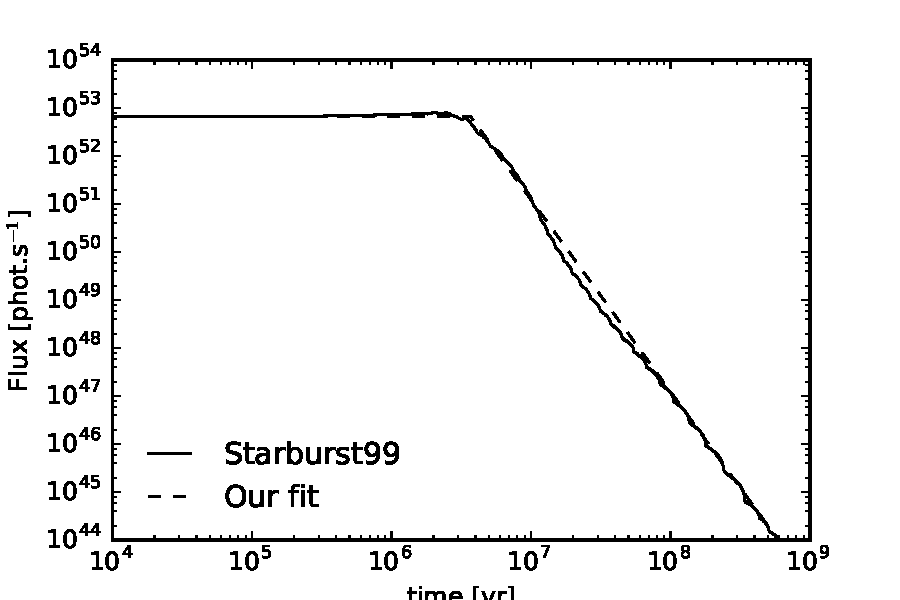
\includegraphics[width=.95\linewidth]{img/03/flux.pdf} 
        \caption{Émissivité ionisante intégrée en fonction du temps}
 		\label{fig:flux}
\end{figure}

Le profil obtenu présente un plateau d'émissivité constante suivie d'une rapide décroissance.
Ce profil peut être raisonnablement approximé par:

$
    S = 
\begin{cases}
    S_0 ,         & \text{if } t < t_{life}\\
    S_0.t^{-4},   & \text{if } t_{life} \leq t < 100.t_{life} \\
    0,   & \text{if } 100t_{life} \leq t
\end{cases}
$

Ce flux correspond au flux d'une population de $10^6M_\odot$.
Ces valeurs seront pondérées au prorata de la masse de la particule stellaire. (Une particule de $10^5M_\odot$ émettra 10 fois moins de photons).

Ce profil d’émission ionisante peut être découper en différents "groupe de photons" (cf section \ref{sec:groupedephotons}).
Il est possible de choisir un nombre arbitraire de groupes, mais il faut prendre en compte que chaque groupe devient l'équivalent d'un fluide dont on veut suivre l'évolution.
Le coût numérique augmente rapidement avec le nombre de groupes. 
J'ai implémenté la possibilité de découper les groupes, en fréquences, mais aussi en temps.
Malgré tout, le ratio cout de calcul sur amélioration des prédictions n'est pas en faveur de l'augmentation du nombre de groupes (dans le cas des résolution considérée pendant ma thèse).
En pratique on prendra un généralement un seul groupe de photons.

L’énergie moyenne d'un photon dans un groupe est calculée de la manière suivante:
\begin{equation}
<E> = \frac{1}{N} \int_{\nu_1}^{\nu_2} N_\nu h \nu d\nu
\end{equation}

et la section efficace d'intéraction:
\begin{equation}
\sigma_E = \frac{1}{N<E>} \int_{\nu_1}^{\nu_2} N_\nu h \nu d\nu
\end{equation}

Pour une IMF TopHeavy, les valeurs obtenues sont:


\begin{table}
\begin{tabular}{l l }
	$<h\nu>$	&  23.42 eV \\
	$\alpha_e$	&  $2.35.10^{-22}$ m$^2$ \\
	$\alpha_i$	&  $1.82.10^{-22}$ m$^2$ \\
\end{tabular}
\caption{Propriété des photon émis par les sources.
\label{tab_photon}}
\end{table}

La table \ref{tab_photon} présente les caractéristique des photons obtenus.


%TODO intégration de l'énergie et de la section efficace


%We found a mean energy of $<h\nu> = 23.42$ eV,
%an energy weighted cross section of
%$\alpha_e = 2.35.10^{-22}$ m$^2$
%and a number weighted cross section of
%$\alpha_i = 1.82.10^{-22}$ m$^2$


%Masse de la population\\
%produit en croix pour correspondre a la masse dans simu\\
%integration seulement sur energy ionisante\\
%
%Multigroupe frequence\\
%multigroup temporel\\


\section{le problème de la masse des étoiles}



%le paramètre de masse des étoiles change la reionization\\
%effet numérique\\
%le rayonnement est piégé dans les cellules\\

Durant mes calibrations, il s'est avéré que le paramètre de résolution de la masse des particules stellaire avait une grande importance dans l'évolution de la fraction ionisée.
Même si celui ci n'a pas d'impact sur la SFR globale, le taux d'ionisation moyen est fortement dépendant de ce paramètre.
Plus la résolution stellaire est élevée, plus la boite réionise tard.


%TODO ajouter les figures cf présentation pp




\section{Les supernovæ}


Les supernovae ont été introduite dans les simulations cosmologiques pour contre balancer "l'overcooling problem".
Sans l'introduction d'énergie dans le gaz par les supernovæ, le gaz s'effondre de manière importante et créer un nombre élevé d'étoiles.
cela mène a un taux de formation stellaire trop important par rapport a ce qui est observé.



\subsection{Le modèle théorique}
il existe principalement deux événement pouvant mener a un explosion de supernovæ : 

\begin{itemize}
\item soit l'étoile est a l'origine suffisamment massive (plus de 8Mo) pour s'effondrer a la fin de sa vie.
\item soit l'étoile n'est pas suffisamment massive (elle va donc mourir en naine blanche) mais dispose de suffisamment de matière a proximité (généralement étoiles double ou le compagnon pas en phase géante rouge) pour que sa masse augmente avec le temps.
la matière accreté va faire passer la masse de cette étoile au dessus de la limite.
\end{itemize}

Les étoiles de plus de 8mo exploses en SN en injectant 1e51 erg dans le milieu\\
Cette injection limite fortement la formation stellaire dans le milieu.\\
modèle sous grille\\
 
\subsection{Les différentes phases}

\begin{itemize}
\item Expansion adiabatique.
Dans la phase d'expansion adiabatique, l'énergie est conservée, le choc est violent et le gaz n'a pas le temps de perdre de l'énergie par radiation.
Dans cette phase, l'expansion est suffisamment rapide pour que la dissipation d'énergie par radiation soit négligeable.
C'est le cas dans le test de Sedov.

\item Snowplow.
Dans la phase snowplow, le choc a suffisamment ralentis pour que le gaz commence a rayonner de l'énergie, l'énergie n'est plus conservée.
Dans ce cas, il se forme un bourrelet de compression dans lequel le gaz est poussé, comme dans le cas d'un chasse neige. 
Les pertes par radiation deviennent importantes. 
\end{itemize}

\subsection{les superbubles}

%A la manière de la percolation des bulles de HII, les bulles de supernovae 

Dans les endroits de formation stellaire, les étoiles ne sont pas isolées mais apparaisent ensemble au sein d'un même nuage de gas.
L'effondrement gravitationnel du nuage mêne a créer un génération d'etoile en un cours laps de temps.
Toutes ces étoiles vont mourrir dans un laps de temps rapproché et ainsi, les differentes supernovae vont injectée de l'energy dans le milieu dans un temsp tres rapproché.
Les différentes bulle vont se rencontrer (a la manière des bulles ionizées) en mener a une bulle plus grande appelée superbuble.


\subsection{les considérations d'échelles}
La façon de gérer les supernovae sera donc fonction de l'échelle que l'on considère.
Dans des simulations très détaillées de galaxies, il sera nécessaire de résoudre la phase adiabatique d'explosion individuelle.
Dans des simulations cosmologiques de la reionisation, l'interet sera plus porté sur la phase snowplow des superbubbles.


\subsection{ Différentes implémentations existantes}



\subsubsection{Navaro and white}


\subsubsection{Stinson et al}



\subsubsection{dubois et Teyssier}

Utilisation de particule fantômes pour simuler les différentes phase

\subsubsection{Dalla Veccia et Schaye}

Modèle probabiliste, injection d'énergie seulement si l'énergie est suffisante pour générer un mouvement suffisant.


\subsection{Mes Implémentations}


\subsubsection{le model thermique}
Le modèle thermique consiste a injecter l'energie sous forme d'energie interne.
Il existe 2 variables d'etat liées a l'energie interne: la pression et la température.
Modifié l'une de ses 2 variables est equivalent.

Dans l'implementation actuelle, la pression est modifiée en utilisant cette conversion:

\begin{equation}
P^{0+} = P^{0-}  + E_0 * (\gamma-1)
\end{equation}

Ce modèle est connu pour avoir de fortes pertes de d'énergie dans le cas ou le refroidissement est autorisé.


\subsubsection{le model cinetique}


Le modèle cinétique consiste a modifier directement la vitesse du gaz autour de l'explosion dans le but de shunter la conversion de l'énergie interne en mouvement.
Ce type de model a été utilisé pour 

Nous avons fait le choix de limiter le nombre de cellules utilisées a 8 correspondant a 1 oct de la structure AMR d'\emma

\begin{equation}
e_{SN} = E_{SN}/8
\end{equation}

Ensuite cette énergie est utilisé pour changer la vitesse du gaz en utilisant : 
\begin{equation}
    \Delta \overrightarrow{v_{gas}} = \sqrt{\frac{2e_{SN}}{\rho_g.dV}} \overrightarrow{u}
    \label{eq_sn_direct}
\end{equation}


\subsection{Test numérique (Sedov)}

%la dérivation des solutions du test de Sedov se trouve :
%chapitre 17 de Shu the physique of astrophysic Volume 2.\\

Dans le but de tester l'implémentation des différents modèles d'injection d'énergie, je l'es ai soumis au test de Sedov.
Ce test est utilisé pour tester le cas d'une explosion parfaite.
Il consiste a relâcher instantanément une quantité d'énergie $E_0$ dans un milieu homogène d'indice adiabatique $\gamma$, de densité $\rho_0$ et de pression $P_0$ (ou de température $T_0$).
Ce brusque changement dans l'état du système créer une discontinuité que le solveur va devoir gérer.

L'avantage de ce test est qu'il dispose d'une solution analytique.
Sedov a exprimé  en 1959 que le rayon de l'explosion en fonction du temps peux s'exprime : %TODO ref

\begin{equation}
r_{(t)}=\left( \frac{E_0}{\alpha \rho_0 }\right)^{1/5} t^{2/5}
\end{equation}


\subsubsection{Sedov évolution temporelle }


parametre du test :
rho=1
p=1e-5
v=0
gamma=5/3


Ce test consiste a suivre l'onde de choc et a s'assurer que son profil et sa position sont correct dans le temps.
On calcul pour chaque cellule sa distance au centre de l'explosion, puis en utilisant un histogramme sur les rayons, pondéré par la valeur du champ que l'on veux analyser, on obtient rapidement le profil radial moyen.
Le résultats présentés utilise l'injection thermique simple (dans une seule cellule).

Le domaine de calcul est en une grille régulière décomposé en $256^3$ éléments  de calcul et le raffinement n'est pas autorisé.

La Fig. \ref{fig:sedov_evol} présentes le trois principaux champs (densité, pression et vitesse radiale) a trois instant différents, comparé a la solution analytique.
On observe un très bon accord en la simulation et le théorie.
Notre méthode d'injection d'énergie est correcte et bien dimensionnée.
%
%\begin{figure}[bth]
%        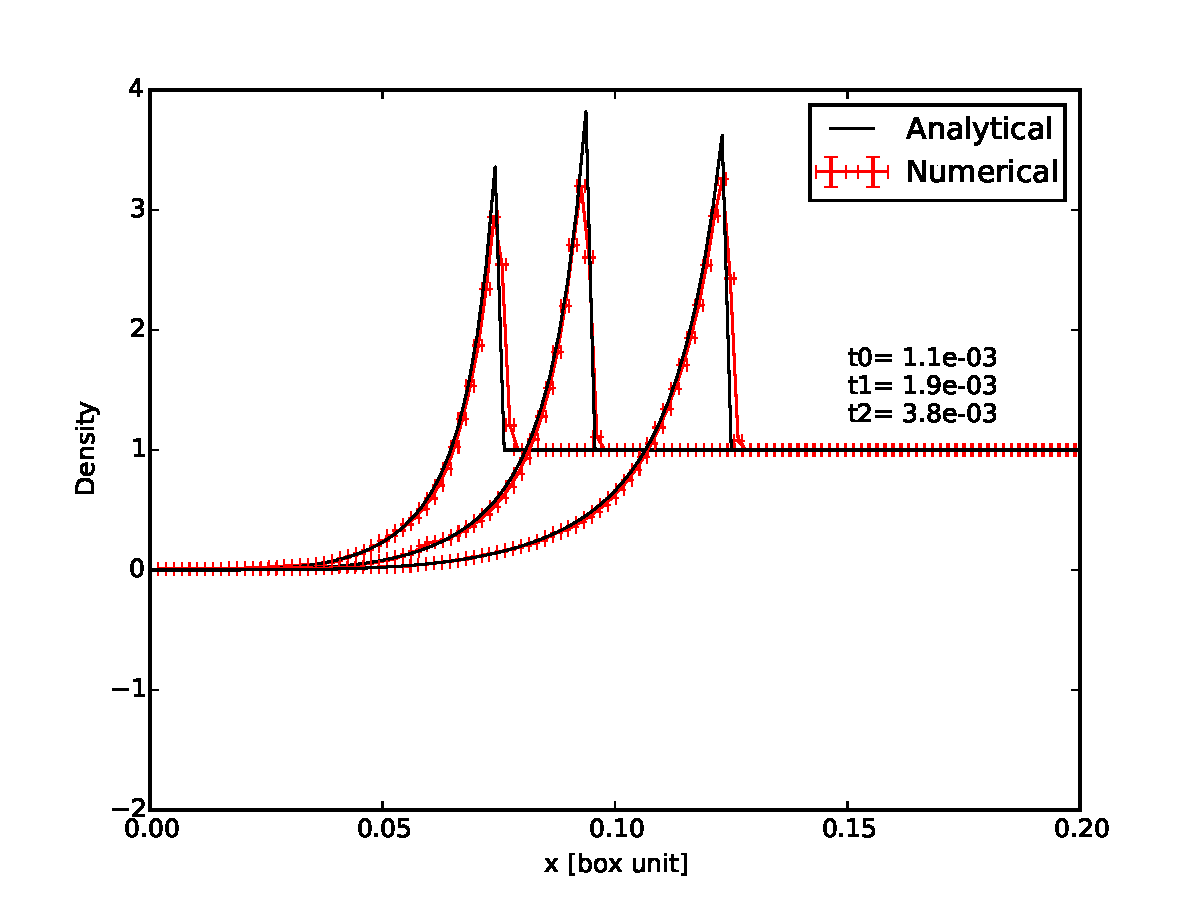
\includegraphics[height=.3\textheight]{img/03/sedov/sedov_evol_8_den_lin.pdf} 
%		\includegraphics[height=.3\textheight]{img/03/sedov/sedov_evol_8_pres.pdf} 
%		\includegraphics[height=.3\textheight]{img/03/sedov/sedov_evol_8_vel.pdf} 
%        \caption{Test de Sedov, évolution des différentes variables d'états. La densité en haut, la pression au milieu et la vitesse radiale en bas.}
% 		\label{fig:sedov_evol}
%\end{figure}

\begin{figure}[bth]
   \begin{minipage}[c]{.46\linewidth}
        \includegraphics[width=\textwidth]{img/03/sedov/sedov_evol_8_den_lin.pdf} 
		\includegraphics[width=\textwidth]{img/03/sedov/sedov_evol_8_pres.pdf} 
		\includegraphics[width=\textwidth]{img/03/sedov/sedov_evol_8_vel.pdf} 

   \end{minipage} \hfill
   \begin{minipage}[c]{.46\linewidth}
		
		\includegraphics[width=\textwidth]{img/03/sedov/sedov_comp_profile_den.pdf} 
		\includegraphics[width=\textwidth]{img/03/sedov/sedov_comp_profile_pres.pdf} 
		\includegraphics[width=\textwidth]{img/03/sedov/sedov_comp_profile_vel.pdf} 

   \end{minipage}

        \caption{Test de Sedov, évolution des différentes variables d'états. La densité en haut, la pression au milieu et la vitesse radiale en bas.        
        Test de Sedov, comparaison des profil radial en fonction des  méthodes d'injection. 
        Densité en haut, pression au milieu et vitesse radial en bas.
        La position et la forme du front d'onde ne dépendent pas de la méthodes d'injection utilisée.
% 		\label{fig:sedovmethod} 
 		}
 		\label{fig:sedov_evol}
\end{figure}



\subsubsection{Sedov comparaison entre les méthodes}

Nous avons vu qu'il existe différents moyens d'injecter de l'énergie dans le solveur hydrodynamique.
Le test présenté ici consiste a vérifié que les différentes méthodes sont équivalentes entre elles.

Nous allons comparer 3 méthodes : 
\begin{itemize}
\item l'injection thermique dans une cellule 
\item l'injection thermique dans un cube de huit cellules
\item l'injection cinétique  dans un cube de huit cellules
\end{itemize}


Ces 3 tests utilisent cette fois ci espace discret de  $128^3$ éléments, mais en autorisant le raffinement sur 3 niveaux.
Le raffinement est effectué sur le gradient de densité, ie une cellule est divisé si le gradient de densité qu'elle contient est supérieur a une certaine valeur.
Cette méthode permet de concentrer le raffinement sur le front de l'onde choc.

La figure \ref{fig:sedovraff} présente le motif de raffinement obtenu pour le test d'injection thermique sur une cellule.
Tout les tests présentent un motif de raffinement similaire.

%\begin{figure}[htpb]
%        \includegraphics[width=.95\linewidth]{img/03/sedov/slice_th_1raf.pdf} 
%        \caption{Test de Sedov, raffinement (mettre la color map) }
% 		\label{fig:sedovraff}
%\end{figure}

La figure \ref{fig:sedovmethod} presente les profils obtenus a un instant donné pour les différentes méthodes d'injection d'énergie et pour les différents champs.
On observe que le front est bien situé au même endroits indépendamment de la méthode.
%Le profil de densité est présenté en échelle logarithmique pour accentuer les difference au niveau du centre. 

%\begin{figure}[htpb]
%        \includegraphics[height=.3\textheight]{img/03/sedov/sedov_comp_profile_den.pdf} 
%		\includegraphics[height=.3\textheight]{img/03/sedov/sedov_comp_profile_pres.pdf} 
%		\includegraphics[height=.3\textheight]{img/03/sedov/sedov_comp_profile_vel.pdf} 
%        \caption{Test de Sedov, comparaison des profil radial en fonction des  méthodes d'injection. 
%        Densité en haut, pression au milieu et vitesse radial en bas.
%        La position et la forme du front d'onde ne dépendent pas de la méthodes d'injection utilisée.}
% 		\label{fig:sedovmethod} 
%\end{figure}


Même si les profils radiaux moyens sont comparables, on observe des différences sur la forme de l'explosion.
La figure \ref{fig:sedovslice} présente une coupe suivant l'axe z de la grille, contenant la cellule d'injection, pour les trois méthodes.
Ces différence sont dues a la grille et a la façon dont les flux sont calculés.
Dans le cas de l'injection thermique, les flux auront tendance à être suivant les axes principaux de la grille.
Ce qui donne ce motif en forme de "+" bien particulier.
Dans le cas de l'injection cinétique, les sont forcés a être dans des directions obliques, a 45°, par rapport a la l'axe de la grille.
Nous avons cette fois si une figure en forme de "x".

%\begin{figure}[htpb]
%        \includegraphics[height=.3\textheight]{img/03/sedov/slice_therm1.pdf} 
%		\includegraphics[height=.3\textheight]{img/03/sedov/slice_therm4.pdf} 
%		\includegraphics[height=.3\textheight]{img/03/sedov/slice_kin.pdf} 
%        \caption{Test de Sedov}
% 		\label{fig:sedovslice}
%\end{figure}



\begin{figure}[htpb]

	\centering
	\subfloat[]{        \includegraphics[width=.45\linewidth]{img/03/sedov/slice_therm1.pdf}} 
	\subfloat[]{		\includegraphics[width=.45\linewidth]{img/03/sedov/slice_therm4.pdf}} \\

	\subfloat[]{		\includegraphics[width=.45\linewidth]{img/03/sedov/slice_kin.pdf} }
	\subfloat[]{		\includegraphics[width=.45\linewidth]{img/03/sedov/slice_th_1raf_cut.pdf}  }

    \caption{Différents motif d'explosion en fonction de la méthodes d'injection.
    Chaque figure représente une tranche d'une cellule d'épaisseur contenant le site de l'explosion.
    (a), (b) et (c) représente le log de la densité avec une colormap quantitative.
    A cause de la grille de calcul, il existe des axes privilégiés pour les flux, il en résulte des motif en croix et ou en losange.
    La figure (d) représente les niveaux de raffinements, le niveau 10 est aligné sur le front d'onde.
    }
 	\label{fig:sedovslice}
\end{figure}



\subsubsection{Conclusion}

La conclusion de ses tests est que les différentes méthodes d'injection sont équivalentes, au moins dans le contexte du test de Sedov.

%OK\\
%mais pas en cosmo

le pas de temps\\


\section{Tests en conditions de production}

Dans le but de tester ces différentes méthodes d'injections dans un contexte cosmologique j'ai réalisé une série de simulations.
Chacune de ces simulation est strictement identique a l'exception de la méthode d'injection d'énergie.
Les paramètres communs a toutes les simulations qui vont suivre sont les suivants:

Elles représentes un volume de 8/h cMpc cube échantillonnées par 256 cube particules de matière noire.
Ce sui mène a une résolution en masse de 3.4 10 6 M0 et une résolution spatiale de 46 ckpc sur la grille coarse.
La grille est raffinée suivant une méthode semi lagrangienne (voir Sec. \ref{sec:raffinement}).

Les condition initiales ont été générées avec MUSIC avec une cosmologie de Planck \citep{planck_collaboration_planck_2016} : 
$\Omega_m=0.3175$, 
$\Omega_v=0.6825$,
$\Omega_b=0.0490$,
$H_0=67.11$,
$\sigma_8=0.830$. 
Les simulations commences a redshift z=150.


Le premier test consiste a essayer les différents feedback avec la même quantité d'énergie injectée, et a mesurer leur impact sur la SFH cosmique.
La figure \ref{fig:sfr_methode} présente les résultats obtenus.
La méthode d'injection cinétique a plus d'impact en condition cosmologique.
Ceci est du a l'introduction de la physique du refroidissement.
La méthode thermique repose sur le principe de conversion de l'énergie interne en énergie cinétique.
La méthode thermique est connue %TODO ref
pour subir d'importante perte d'énergie.
La méthode cinétique outre passe cette conversion et mets directement le gaz en mouvement.

%TODO parler du feedback radiatif

\begin{figure}[bth]
        \includegraphics[width=.95\textwidth]{img/03/sedov/SFRmethode.pdf} 
        \caption{SFH cosmique en fonction de la méthode d'injection.
        Les méthodes n'impactent pas le milieu de la même manière
        }
 		\label{fig:sfr_methode}
\end{figure}

Nous aurons donc tendance préférer la méthode cinétique par la suite, vu que celle ci est plus efficace a nos échelles.
Le deuxième test consiste a utilisé la méthode cinétique et a varier la quantité d'énergie injectée.
La figure \ref{fig:sfr_egy} présente les résultats obtenus.
On y observe que plus on injecte d'énergie, plus la SFR instantanée diminue.
Ce qui est le comportement attendus puisque plus les supernovae sont puissante, plus les sur-densités de gaz sont "cassées", et donc plus difficile il devient de former de nouvelles étoiles.

\begin{figure}[bth]
        \includegraphics[width=.95\textwidth]{img/03/sedov/sneff_SFR.pdf} 
        \caption{SFH cosmique en fonction de la quantité d'énergie injectée. 
        Plus la quantité d'énergie injecté est importante, plus le taux de formation stellaire diminue.
        }
 		\label{fig:sfr_egy}
\end{figure}



Un troisième test consiste a injecter une certaine quantité d'énergie par supernovae, et a faire varier l'efficacité de formation stellaire.
En effet plus on forme d'étoiles et plus le feedback devient important, mais plus il y a de feedback, moins il est facile de former de nouvelles étoiles.
Le couplage entre feedback et formation stellaire n'est pas clair et mérite d'être exploré.
La figure \ref{fig:sfr_sfe} présente ce test pour trois efficacité de formation stellaire avec un modèle de feedback cinétique et une efficacité de supernovae de 100 \%.
On observe un fort couplage entre feedback et formation stellaire, a tel point que pour une efficacité de formation stellaire de 10\% le feedback mène a une SFH décroissante.

\begin{figure}[bth]
        \includegraphics[width=.95\textwidth]{img/03/sedov/SFR_sfeff.pdf} 
        \caption{SFH cosmique en fonction de l'efficacité de formation stellaire.
        Toutes les simulation utilise la même méthode d'injection et la même quantité d'énergie.
		L'effet du couplage est bien présent.
        }
 		\label{fig:sfr_sfe}
\end{figure}

Une observation importante par rapport au deuxième test est qu’indépendamment de la quantité d'énergie injectée, et que même si la SFR est significativement impacté, l'histoire d'ionisation reste quasiment constante (cd fig \ref{fig:xion_sneff}).


\begin{figure}[bth]
        \includegraphics[width=.95\textwidth]{img/03/sneff_xion.pdf} 
        \caption{Malgré une SFH différente (voir figure \ref{fig:sfr_egy}), l'histoire d'ionisation est conservée en changeant la quantité d'énergie injectée.
        }
 		\label{fig:xion_sneff}
\end{figure}

Cet effet est inattendu car si la quantité d'étoiles diminue, la quantité de radiation diminue d'autant, et donc la fonction d'ionisation globale devrait être impacté.
Or ce n'est pas ce qui est observé ici.
Dans le but d'explorer cet effet, nous allons nous concentrer dans la suite a une étude galaxies par galaxies.














%%\include{multiToC} % <--- just debug stuff, ignore for your documents
%\chapter{Les Halos}

L'étude des simulation se fait souvent halos par halos.
Quand on cherche a déterminer es propriétés des galaxies, un paramètre important est leur masse.
Comme le gaz suit la dynamique des baryons, les galaxies sont situées dans les surdensités de matière noire.




\section{La detection des halos}

L'objectif d'un halo finder est de detecter les surdensités dans le champs de matière noire.
Comme nous l'avons vu plus tot, (TODO ref) le champ de matière noire utilise une représentation sous forme de particules.

J'ai principalement utilisé l'algoritme Friend Of Friend pour detecter les sur densités.

FOF retourne une liste de position de halo, une liste permettant de lier les particules detecté aux halo.

\subsection{Le rayon de Viriel}
Approximation par le R200:
\begin{equation}
R_{200}=\frac{3\cdot M_{FoF} }{4\pi\cdot 200 \bar{\rho} }
\end{equation}


\subsection{Le problème de la forme des halos}
Fortement non viriallisé a z=6\\
beaucoup de dynamique et merger dans les filemments

\begin{figure}[bth]
        \includegraphics[width=.95\textwidth]{img/03/part_halo_R200.pdf} 
        \caption{La détection des halos par FOF peux être difficile au moment de la reionization car les structure ne sont pas Virialisée
        }
 		\label{fig:part_halo}
\end{figure}

\begin{figure}[bth]
        \includegraphics[width=.95\textwidth]{img/03/part_cells.pdf} 
        \includegraphics[width=.95\textwidth]{img/03/part_cells_fine.pdf} 
        \caption{La detection des halo par FOF peux être difficile au moment de la reionization car les structure ne sont pas Virialisée
        }
 		\label{fig:part_halo}
\end{figure}




\subsection{association dans le R200}

On cherchera a associer les galaxies  (surdensité d'étoiles) aux halos.
La première méthode consiste a utiliser l'approximation du R200.
Il faudra associer, la matière noire, le gas et les étoiles compris a l'intérieur d'une sphere de rayon R200.

Il sera possible d'utiliser une méthode comparable sur la grille, en utilisant les centres de cellule a la place de la position des étoiles.
Comme les particules de matière noire  données par FoF ne represente pas le meme volume, dans un soucis de cohérence, on appliquera cette méthodes a la matière noire également.

Le méthode est la suivante:

\begin{itemize}
\item générer un KDtree sur les particule de matière noire / les étoiles / la grille AMR
\item Faire une recherche sphérique autour de la positions des halo, sur un rayon de R200
\item stocker les indices dans une structure
\end{itemize}

nous avons donc la possibilité, pour chaque halo, de connaitre n'importe qu'elle grandeur comprisent dans son R200.


Pour les petits halos, peu résolus, la taille des cellules peu être grandes par rapport au R200.
Pour minimiser l'erreur commise, la grille AMR pourra être projeter sur une grille régulière de resolution arbitraire.
Cette méthode permettra d'associer des sous parties de cellules aux halo et améliorera la precision global de l'association.

\subsection{Association "fine"}
Dans le but d'améliorer ces problèmes d'identification dans les halos fortement non virialisé, j'ai développer une méthode pour associer plus précisement les halos et la grille.


la méthode consiste a :
\begin{itemize}
\item générer un KDtree sur la grille
\item pour chaque particule d'une halo, trouver la plus proche cellule
\item filtrer les cellules doublons
\end{itemize}

\section{Étude de la composition dans le R200}


\subsection{La fonction de masse HMF}

\subsection{La masse d'étoiles en fonction de la masse de matière noire + Stellar mass function}
Plus un halo est massif, plus celui ci va contenir d'étoiles.



\subsection{La formation stellaire en fonction de la masse du halo}
Connaissant, a un instant donné, les étoiles appartenant a chaque halo, il est possible de déterminer leurs ages, et donc de connaitre l'histoire de formation stellaire de chaque halo.
Nous allons voir que la masse 

\subsection{La fraction baryonnique}
La fraction baryonique est une grandeur importante pour caractériser un halo.
En effet, le rayonnement n'interagit qu'avec les baryons et plus un halo aura de baryon, plus le rayonnement aura de difficulte a s'en echaper.

\begin{equation}
f_b = \frac{M_* + M_{gas} }{M_{DM} + M_* + M_{gas} }
\end{equation}




\section{Etude au R200}

\subsection{Healpix}
\label{sec:healpix}

Healpix est un outils qui permets de répartir des points de manière uniforme sur la sphere.

\begin{figure}[bth]
        \includegraphics[width=.95\linewidth]{img/03/healpix.jpg} 
        \caption{Exemple de sphere HealPix}
 		\label{fig:HealPix}
\end{figure}

Projection sur la grille AMR
 - utilisation du KD tree
 - nearest neighbhoor
 - récupération des cellules sur la sphere
 

\subsection{Détermination des flux au $R_{200}$}
\label{sec:healpix}

Projection des vecteurs surla normale des cellules de la sphere.

Une question importante dans l’étude de réionisation est la quantité de rayonnement ionisant sortant des halos.
Nous avons vu que le rayonnement interagis les baryons


Pour déterminer les flux autours de chaque halo, il est nécessaire de les englober d'une sphère.
Cette sphère serra discrétisée a l'aide de Healpix (TODO ref) un outils qui permets de répartir des points de manière uniforme sur une surface sphérique (Fig. \ref{fig:HealPix}).
Une fois la sphère générée, on la centrera sur la position du halo, et on la redimensionnera de telle manière a ce qu'elle corresponde aux R200 du halo en question.
Ensuite, pour chaque point de la sphère Healpix, on effectuera une recherche de plus proche voisin, pour déterminer avec qu'elle cellule l'associer.

Nous connaissons maintenant l'ensemble des cellules au R200 de chaques halos.

\subsection{la vitesse du gas au R200}



\subsection{le flux radiatif au R200}
en utilisant cette technique sur 


\section{Influence du feedback stellaire sur la reionization}







\subsection{fraction d'echapement}

%fonction de luminosité 

%
%\cleardoublepage
%\ctparttext{Cette partie est liée a la publication présentée en annexe\,\ref{pap:c}.\medskip
%
%\emph{"Influence of reduced light speed approximation on reionization fronts speed in cosmological RHD simulation"\\}\medskip
%
%Nicolas Deparis, Dominique Aubert et Pierre Ocvirk.
%En  préparation.
%}
%\part{Influence du l'approximation de vitesse de la lumière réduite sur la propagation des fronts d'ionisation}
%\chapter{Introduction au calcul des cartes de reionisation}


Nous avons abordé dans la partie précédente une étude centré sur les halos.
Cependant les contraintes observationnelles sur la reionization sont sur l'\ac{IGM}

Les cartes de redshift de reionization sont de outils important pour l'étude de la reionization dans son ensemble.
Ces cartes sont constituée en chaque point de l'espace, du redshift au quel chaque cellule et passer au dessus d'un certain niveau d'ionisation moyen.

Il est possible de définir deux façons d'allouer un redshift.
Il est possible de considérer la première, ou la dernière ionization.

Dans le cas de la première ionisation, la valeur ne devra être mise a jour qu'une seule fois au moment du passage du seuil.
Pour ce faire, toutes les cellules seront initialisées a une valeur impossible (prenons -1 pour l'exemple).
La mise a jour ne se fera donc qu'a la condition que la fraction d'ionisation soit superieure au seuil ET que la valeur actuelle du redshift d'ionisation soit -1.
Ainsi la valeur ne sera pas remise a jour a chaque pas de temps ou la cellule sera ionisée. 

Dans le cas de la dernière ionisation, la valeur du redshift sera mise a jour, tant que la fraction d'ionisation de la cellule est inférieure au seuil.
Ainsi, si un cellule recombine, le valeur de son redshift associé sera de nouveau mise a jour, et la mise a jour stoppera a chaque passage au dessus du seuil.

L'implémentation est présenté sur le Listing \ref{lst:majz}.

\begin{lstlisting}[float=bth,language=c,frame=tb,caption={Mise a jour du redshift de reionisation},label=lst:majz]
  #define THRESH_MAP (0.5)

  if(cell.xion<THRESH_MAP)
    cell.t_last_xion=current_z;

  if( (xion>=THRESH_MAP) && (cell.t_first_xion==-1) )
    cell.t_first_xion=current_z;
\end{lstlisting}


Dans le cas d'une grille AMR, l'organisation de la grille est ammenée a évoluer.
La question du raffinement/deraffinement  se pose alors.
Si dans le cas du raffinement, l'injection directe du redshift de la cellule mère ne pose pas de problème particulier, les choses sont différentes lors du déraffinement.
En effet, dans EMMA, quand une cellule est deraffinée la valeur moyenne des 8 cellules filles est injectée dans la cellule mère.
Le problème est que les redshift ne doivent pas être moyennés.
La simulation, et les processus physiques qui y ont lieu, sont calculé par rapport au temps.
Nous avons vu dans la partie \ref{sec:friedman} qu'il existe un lien non trivial entre le redshift et temps (l'age de l'Univers).
Pour répondre a ce problème, j'ai fait le choix de travailler non pas avec le redshift mais avec l'age de l'Univers au moment de l'ionisation de la cellule.
Les cartes de temps seront converties en cartes de redshift en post traitement en utilisant les mèmes paramètres cosmologique que ceux utilisés en interne de la simulation.

%TODO DECRIRE LES CARTES


Motifs concentrique autour des sources\\

forme de papillon.\\

trace des fillemmment\\


\begin{figure}[htpb]
        \includegraphics[width=.95\linewidth]{img/04_mapreio/map_z_c1.pdf} 
        \caption{Exemple de carte de redshift de réionisation généré par EMMA.
        Il s'agit d'une tranche d'une cellule d'épaisseur.
        }
 		\label{fig:zmap}
\end{figure}

\section{Cartes de vitesse d'ionization}

A partir des cartes de redshift de reionisation, il est possible d'annalyser la vitesse de propagation de l'ionisation dans la simulation.
L'idée est la suivante:
En utilisant le fait que les cartes de temps nous donnent un temps pour chaque point de l'espace, il est possible quel est le temps qu'il s'est ecoulé entre la reionisation de deux cellules adjacente, et donc de connaitre la vitesse a laquelle le front d'ionisation les a traversées.

En pratique, la vitesse des fronts sera calculée en calculant le gradient de la carte de temps d'ionisation.
Une fois de plus il est necessaire de travailler avec le temps et non le redshift, ce qui ajoute un argument en faveur du choix de travailler en temps et non en redshift.
De plus en prenant diretement le gradient, on obtient le temps mis par le front pour parcourir une distance dx correspondant a la taille de la cellule.
Il faudra donc prendre l'inverse du gradient pour obtenir une vitesse.

La vitesse des fronts d'ionisation $V_{reio}$ est définis comme :

\begin{equation}
V_{reio}  = \left | \frac{1}{ \vec{\nabla} t_{reio}} \right| .
\end{equation}


Le calcul du gradient étant problématique au niveau des interfaces entre niveaux de raffinement, les études présentées ici ont été réalisée en projetant la grille \ac{AMR} sur le niveau coarse, de manière a n'avoir qu'un seul niveau, et a supprimer ces interfaces.

L'objectif est de comparer la vitesse des fronts d'ionisation a la vitesse de la lumière.
Or il reste un problème a régler, la carte de vitesse obtenue est en unité comobile, alors que la lumière voyage avec une vitesse physique.
Pour contrer ce problème, le gradient devra être pondéré par la valeur du facteur d'expansion de la cellule associée.
On obtiendra ce facteur par intégration de la cosmologie, de la même façon que pour transformer la carte de temps en carte de redshift.

Au final, le calcul du gradient sera discrétisé de la manière suivante:

\begin{equation}
\vec{\nabla} t_{reio}^i \approx \frac{t^{i+1}  - t^{i-1}}{2a^i \left( x^{i+1}  - x^{i-1} \right)}.
\end{equation}

ou $i$ est l'indice de la cellule, a le facteur d'expansion, $t$ le temps d'ionisation et $x$  la position de la cellule.

Un exemple de carte obtenue est présenté Fig. \ref{fig:vmap}.

\begin{figure}[htpb]
        \includegraphics[width=.95\linewidth]{img/04_mapreio/map_v_c1.pdf} 
        \caption{Exemple de carte de vitesse de fronts générée par la méthode du gradient.
		 Cette carte correspond a la même tranche que celle présenté Figure \ref{fig:zmap}
        }
 		\label{fig:vmap}
\end{figure}

TODO DECRIRE LES CARTES\\

\section{vitesse en fonction du redshift}
Nous avons associé a chaque cellule un redshift et une vitesse.
Regardons maintenant comment se comporte l'un par rapport a l'autre sur la Figure. \ref{fig:speedz}.

On observe que la gamme de vitesse est comprise entre 1e-4 et 1e-1 sur une grande partie du processus (avantz=8).
ceci est suivis d'un pic de vitesse puis d'une chute brutale correspondant a l'instant ou toutes les cellules sont reionisées.

\begin{figure}[htpb]
        \includegraphics[width=.95\linewidth]{img/04_mapreio/speedreio_z_c1.pdf} 
        \caption{Vitesse d'ionisation en fonction du redshift
        }
 		\label{fig:speedz}
\end{figure}


\section{accélération}
Il est possible de dériver une seconde fois la carte de temps d'ionisation pour obtenir une carte d'accélération des fronts.
Cette accélération est une accélération spatiale.
Il s'agit de la variation spatiale de vitesse.
La carte obtenue est présenté sur la figure \ref{fig:accz}.

\begin{figure}[htpb]
        \includegraphics[width=.95\linewidth]{img/04_mapreio/map_acc_c1.pdf} 
        \caption{Carte d'accélération des fronts d'ionisation.
        }
 		\label{fig:acc}
\end{figure}





De la même manière que précédemment, il est possible de lier les cartes de vitesses et d'accélération
\begin{figure}[htpb]
        \includegraphics[width=.95\linewidth]{img/04_mapreio/v_gradv_c1.pdf} 
        \caption{Accélération des fronts d'ionisation en fonction de leur vitesse.
        Plus un front va vite, plus il accélère.
        }
 		\label{fig:accspeed}
\end{figure}


figure \ref{fig:accspeed}
Je n'ai pas réussi a identifier l'origine de la bosse
On y observe que plus un front est rapide, plus il accélère.
Ce qui conforte l'idée que la reionisation est un processus qui s'emballe.




%\chapter{Influence du l'approximation de vitesse de la lumière réduite sur la propagation des fronts d'ionisation}
\chapter{Vitesse de la lumière et vitesse des fronts d'ionisation.}

J'ai utilisé l'outil développé dans la section précédente pour comparer des simulation identiques a l'exception de l'approximation de la vitesse de la lumière réduite (Reduce Speed of Light RSLA).

Comme abordé dans la section sur le solveur radiatif %TODO ref
le calcul de la radiation est couteux en terme de ressource de calcul.
Ceci car la condition de Courant impose d'exécuter un grand nombre de pas de temps.
L'idée de la RSLA est que la vitesse de la lumière est significativement plus rapide que la vitesse des autres processus a l'oeuvre dans la simulation.
Partant de ce constat, meme en la réduisant d'un facteur $N$, cette vitesse devrait rester significativement supérieure, et mener aux meme résultats.
En divisant la vitesse par un facteur $N$, on peux augmenter la taille du pas de temps par le meme facteur, et donc diminuer le nombre de pas de temps total et le cout global du solveur radiatif.
L'objectif de cette section est d'explorer l'impact de ce facteur sur la vitesse des fronts d'ionisation.
Nous verrons que la réionisation est un processus qui s'effectue en deux phases, et que en fonction de la RSLA, l'une ou l'autre est affectée.



\begin{figure}[htpb]
        \includegraphics[width=.95\linewidth]{img/04_mapreio/z_rsla.pdf} 
        \caption{REdshift de reionisation en fonction de la RSLA
        }
 		\label{fig:zrsla}
\end{figure}

Figure \ref{fig:zrsla}



\begin{figure}[htpb]
        \includegraphics[width=.95\linewidth]{img/04_mapreio/PDF_v_reio.pdf} 
        \caption{Densité de probabilité de trouver une vitesse dans la boite.
        }
 		\label{fig:pdfv}
\end{figure}

figure \ref{fig:pdfv}



\begin{figure}[htpb]
        \includegraphics[width=.95\linewidth]{img/04_mapreio/avg_reionization_speed.pdf} 
        \caption{Vitesse moyenne des fronts en fonction du redshift.
        }
 		\label{fig:vreioz}
\end{figure}


figure \ref{fig:vreioz}.


%
%\cleardoublepage
%\ctparttext{Cette partie est liée a la publication présentée en annexe\,\ref{pap:z0}.\medskip
%
%\emph{"Connecting the reionization history of galaxies to their $z=0$ properties"}\medskip
%
%Dominique Aubert, Pierre Ocvirk et Nicolas Deparis.
%En  préparation.
%
%}
%\part{COsmic DAwn EMMA}
%\label{sec:CODAEMMA}

\section{Intro}

%Lettre donc partie courte.

Cette partie repose sur une lettre qui s'inscrit dans une stratégie de travail a long terme.
Elle a pour vocation de présenter la simulation "CODA II EMMA" ainsi que les premiers résultats obtenus.
Ces résultats utilise deux simulation pour faire le lien entre la période de réionisation et l’époque actuelle.
Cette étude montre que les halos les plus massifs a z=0 sont réionisé plus tôt que le reste de l'Univers.

%Objectif connaitre le Z reio des halo en fonction de leur masse.
%Sur grosse simu donc beaucoup de stats

%\subsection{Présentation de la simulation CODA II EMMA}

\subsection{Conditions initiales}

Les conditions initiales ont été générée par la collaboration CLUES (Constrained Local UniversE Simulations).
L'objectif est de retrouver dans la simulation des structures aillant des caractéristiques proches de ce qui est observé dans l'univers local.
On cherchera par exemple a obtenir un couple Andromède - Voie Lacté avec des masses, distances et vitesses relative en accord avec les contraintes actuelles.

%cosmo

Le volume de $\left( 64/h cMpc \right) ^3$ est échantillonné par $2048^3$ particules de matière noire.
Ce qui mêne a une résolution en masse $3.4 \cdot 10^6 M_\odot$ et une résolution spatiale de 46 ckpc sur la grille coarse.
Ces paramètres permettent d'explorer la gamme de masse de halos compris entre $10^8 M_\odot$ et  $10^{13}M_\odot$.

Ces conditions initiales sont une version basse résolution de celles de la simulation CODA I%TODO ref
réalisé avec le code RAMSES CUDATON %TODO ref
initialement en $4096^3$.
La perte de un niveau de résolution est compensé par l'utilisation de l'AMR de EMMA.

L'objectif est de pouvoir faire une comparaison directe entre ces deux simulations (CODA I RAMSES CUDATON vs CODA II EMMA) dans un avenir proche.

%différences avec CODA I RAMSES CUDATON et future comparaisons
%8x moins résolue en masse 
%Mais mieux résolue en dx


\subsection{Présentation des simulations}

A partir de ces conditions initiales plusieurs simulations ont été réalisées:

\begin{itemize}
\item Une simulation matière noire pure réalisée avec Gadget %TODO ref
exécutée jusqu'à redshift z=0.
Cette première a pour objectif de suivre l'évolution des structures.

\item Et une simulation en RHD entièrement couplé avec EMMA poussée jusqu'à z=6 à la fin de la simulation.
Cette dernière a été exécutée sur 32768 cœurs CPU et 4096 GPU du calculateur TITAN.
Elle a pour but d'avoir une représentation complète de l'époque de réionisation.
\end{itemize}



\subsection{projection a z=0}

L'objectif est de créer un lien entre ces deux simulations.
La simulation matière noire a servi a créer un arbre de fusion (merger tree) des halos, permettant de suivre les histoires de formation des halos du début de la simulation jusqu'à nos jours.

En considérant que le couplage entre la matière noire et les baryons et faible, la comparaison entre les catalogues de halos des deux simulations pris a la même époque peux être réalisé directement.


les 2 méthodes :

- Centre de masse pris dans le merger tree
- moyenne du t des particules



\subsection{Résultats}



%
\cleardoublepage
\ctparttext{Cette partie est liée proceeding de conférence présentée en annexe\,\ref{pap:visu}.\medskip

\emph{"Immersive 3D visualization of astronomical data"}\medskip

A. Schaaff, J. Berthier, J. Da Rocha, N. Deparis, S. Derriere, P. Gaultier, R. Houpin, J. Normand et P. Ocvirk.
}
\section{Introduction a la visualisation de données}


Nous avons abordé en guise d'introduction un principe de base de la méthode scientifique: le cycle \textit{Observation -> Théorie -> Expérience}.
La visualisation représente l'étape de bouclage de ce cycle  puisque qu'elle consiste à observer le résultat de l'expérience de simulation.
Elle est importante car elle permet d'obtenir énormément d'informations facilement et rapidement.
Le cerveaux humain est efficace pour identifier les motifs qui se détache visuellement de leur environnement.
Elle permet une première approche qualitative qui va ensuite permettre de cibler une seconde approche plus quantitative.

%Par exemple, on peux utiliser une visualisation de la distribution de gaz autour de certaine galaxie pour identifier leur environnement, et ensuite l'étudier un fonction de la masse du halo hôte.
%La visualisation représente la première étape dans l'observation de la simulation.
%leurs forme, pour ensuite chercher a quantifier leurs forme en fonction de leurs halo hote.
%On peut facilement observer a l'oeil les motifs en forme de papillon des bulles d'ionisation.
%Ou la structure en réseau de la matière a grande échelle.
%La visualisation de donnée scientifique 


%pour qui?
En fonction du publique auquel s'adresse la visualisation, l'information utile sera différente et l'accent sera mis sur différents aspect.
%Il existe tout un panel de visualisations possible, et avant même de définir un but il faut définir une cible, car les outils ne seront pas les mêmes en fonction de la cible a laquelle ils s'adressent.
On distinguera principalement trois catégories de public:

\begin{itemize}
\item Le grand public. 
 
Il sera principalement touché par les images de vulgarisations que l'on peut trouver sur internet ou dans les magasine.
Ce type d'image n'a pour seul but que d'être artistique et agréable a regarder.

\item L'éducation.

Les images a vocation éducatives se doivent aussi d'être belles, mais elles doivent également comporter une partie informatives.
Elle doivent contenir une certaine dose d'information supplémentaire par rapport aux images purement artistique.

\item Les professionnels.

Enfin, les outils de visualisation pour les professionnels disposent généralement de tous les outils nécessaire à la quantification de l'information.
On pourra par exemple analyser différents champs physique, sous différents angles, changer les échelles de couleurs, etc.

\end{itemize}


% L'éducation 
%Ratio équitable entre qualification et quantification

%/ La vulgarisation
%Qualification principalement 
%il est important de créer des belles image

%Aligner des 1 et des 0 sur des gros ordinateur, n'a vraiment de sens que si il représente quelque chose.
%Le mot important dans cette phrase est représentation.
%Il est nécessaire, en recherche de visualiser ce qui se passe dans les simulations pour comprendre et qualifier les phénomènes avant de pouvoir les quantifier.
%Cette cible aura besoin d'outils pointu aillant pour principal objectif la quantification.

Le principal défi de la visualisation des simulations cosmologique est la quantité de données qu'elles représente.
Si il est possible de faire des rendu pré-calculés d'images, il est encore impossible d'avoir une représentation en temps réel de simulation de taille moyenne.
Pourtant il existe des techniques (dans le monde des jeux vidéo par exemple) permettant d'afficher dynamiquement des univers en 3 dimensions gigantesque de manière fluide sur des machines grand public.
Je pense qu'il y a de quoi s'inspirer de ce coté la.

Nous avons vu %TODO ref
qu'il existe deux types de représentation de la physique dans la simulation : la grille et les particules.
Ces deux représentation utilisent chacune des techniques de visualisation particulières.
Dans la suite de cette partie nous allons aborder séparément ces types de représentations et survoler les contraintes et les techniques associées a chacune.

Nous commencerons par aborder la visualisation de données sur grille, puis dans un second temps nous nous concentrerons sur la représentation des particules.
%Pourquoi

%Le monde de la 3D.
%Les simus, les moteurs de jeux video, les SFX de films,
%La 3D est partout.
%Les monde des simulation peux s'en inspirer.

\section{Projeter une grille AMR}

EMMA travail dans un espace en trois dimensions.
Nous cherchons ici à créer une image des résultats produit par EMMA.
En sortie d'EMMA, l'information est sous forme de liste de cellules \ac{AMR} disposant d'une position et d'une taille, dans un espace en trois dimensions.
Une image est composée d'une matrice à deux dimensions de pixels, généralement réguliers en forme et en taille.
Il est donc nécessaire d'effectuer une transformation entre ces deux représentations.
Cette transformation (on parlera de projection) mène a la perte d'une dimension, qui sera réduite a l'aide de lignes de visées.


\subsection{Le tirage des lignes de visées}

%La représentation d'un environnement virtuel a 3 dimensions passe toujours par la création d'une image a deux dimensions.
Il existe différents types de méthodes de projections qui dépendent de la gestion des lignes de visées.
Dans la suite de ce chapitre nous allons développer deux d'entre elles: la projection en perspective et la projection orthogonale (Fig \ref{fig:raycast_projection}).

\paragraph{La projection orthogonale} correspond a l'approximation de grande distance.
Les rayons sont parallèles entre eux et le cube de données est comme "écrasé" ou "imprimé" suivant un axe donné.
Cette projection est moins naturelle, dans le sens où elle ne correspond pas a ce que nous avons l'habitude de percevoir, mais elle a l'avantage d'être relativement simple a mettre en œuvre.

\paragraph{La projection en perspective} correspond au cas l'observateur est ponctuel et au centre d'une sphere, les rayons lumineux lui arrive radialement.
C'est la projection qui se rapproche le plus de la vision "naturelle".

\begin{figure}[bth]
    \center
    \subfloat[Orthogonale]{\includegraphics[width=0.45\textwidth]{img/04/raycast_ortho.png}}%
    \qquad
   	\subfloat[Perspective]{\includegraphics[width=0.45\textwidth]{img/04/raycast_perspective.png}}%
    \caption{Les deux types de projections que nous allons aborder.}
 	\label{fig:raycast_projection}
\end{figure}


\subsection{La réduction des lignes de visées}

Avant d'aborder le tirage des lignes de visées a proprement parlé, voyons rapidement comment les réduire une valeur unique pour effectuer la projection.
Il existe différentes façons de réduire les lignes de visées, en voici quelques une que j'ai pu utiliser:

\begin{itemize}
\item La moyenne ou la somme ont l'avantage d'être facilement implémentable et de garder l'information sur toute la ligne de visée.

\item Le maximum permet d'augmenter significativement le contraste, rendant les images visuellement plus intéressante que la moyenne/somme mais en contre partie certaines projections peuvent présenter des artefacts indésirables.

\item L'épaisseur optique permet de garder de l'information sur toute la ligne et d'être une représentation avec une signification physique car elle utilise les équations de transfert du rayonnement.
Cependant elle est plus gourmande en ressources.
Pour faire de la visualisation pure on pourra utiliser une expression du type:
\begin{equation}
v= \sum e^{-x}
\label{eq:epop}
\end{equation}
Et on pourra également être plus quantitatif en utilisant les vraies équations physique mais il faudra utiliser plusieurs champs simultanément. %TODO ref

\item D'une manière générale, toute transformation permettant d'obtenir une seul valeur a partir d'une série

\end{itemize}

%Une des méthodes les plus facile consiste a prendre la moyenne ou la somme de la ligne, cette méthode présente l'avantage de représenter l'ensemble de la ligne.
%Il est également possible de prendre les maximum de la ligne, cette méthode augmente significativement le contraste, au point que certaines projections peuvent présenter des artefacts indésirables.

%Une troisième méthodes légèrement plus physique consiste a utiliser les équations de transfert du rayonnment pour determiner l'epaisseur optique de la ligne

%Enfin, il est possible d'utilisé la réelle expression de l'epaisseur optique, prenant en compte densité, température, ionization et vitesse du gaz.
%(TODO)

\section{Projection orthogonale}

La projection orthogonale est la plus directe car tout les rayons sont parallèles entre eux et suivent un axe de la grille.
Comme la grille est ici composée de cellule de différentes taille, il faut prendre en compte l'étendue spatiale de chaque cellule de manière individuelles.

J'ai développé une méthode de projection d'\ac{AMR} sur une grille (2D ou 3D) de taille arbitraire en utilisant des histogrammes.
Ces fonctions étant très bien optimisées, la performance de génération des cartes/cubes est généralement satisfaisante (de l'ordre de quelque secondes pour un cube de $1024^3$ avec les fonctions histogramme de Numpy).
L'idée est de considérer les cellules \ac{AMR} comme des particules et de les projeter niveau par niveau.


%Prenons l'exemple de la densité sur une grille non raffinée utilisant le format de sortie d'EMMA.
%Une grille 2D quelconque est représenté par le couple $x,y$ étant les positions du bord inférieur gauche des cellules, $l$ étant le niveau des cellules et $d$ étant le champs a représenter (prenons par exemple la densité).

Par exemple, prenons comme objectif de projeter la densité de gaz provenant d'une grille \ac{AMR} 3D de niveau de base $L_{0}=8$ sur une matrice 2D $256^2$.
En réalisant un histogram 2D, sur les positions $x$ et $y$ des cellules, on obtient directement un projection suivant l'axe $z$ de la grille \ac{AMR}.
Les valeurs de toutes les cellules aillant des positions comprise dans un intervalle (x+dx,y+dy) seront automatiquement ajoutées au pixel correspondant.

Cependant, dans le cas d'une grille raffinée, il est nécessaire de prendre en compte une pondération pour les cellules raffinées.
Le volume d'une cellule est définis en fonction de son niveau $dV= 2^{-3L}$, et son poids $w$ en fonction de la valeur $\rho$ à projeter sera $w = \rho \cdot dV$.
L'image finale sera alors obtenue en réalisant un histogramme 2D pondéré par $w$.

%En réalisant un histogram 2d de x et y pondéré en masse.

%En considérant le centre des cellule $(x' = x+dx(L) /2)$ et en ajustant le bin de l’histogramme sur la taille de la grille on peux projeter un niveau rapidement.

%\begin{lstlisting}[float=bth,language=python,frame=tb,caption={lprojection de l'AMR par la méthode des histogramme Numpy},label=lst:useless]
% import numpy as np
% h,binX,binY=np.hystogram2d(x,y,weight=dv)
%\end{lstlisting}
%u h est une matrice 2d representant la projection.
%Lorsque l'AMR d'entrée contient plusieurs niveaux, il est possible de projeter les cellules niveau par niveau.


Ceci n'est valable que dans le cas d'une projection sur le niveau de base de la grille \ac{AMR}.
Cependant il est possible de projeter la grille a une résolution supérieure.
Prenons par example pour une grille contenant de niveau $L_{0}=8$ raffinée une fois.
Pour obtenir une image $512^2$, on projettera d'abord toutes les cellules de niveau 8 (et seulement ces cellules) pour obtenir une matrice $256x256$.
On agrandira cette matrice avec des opérateurs de changement de grille (cf Section \ref{Opérateurs de changement de grilles}).
%La méthode la plus naturelle consiste utiliser une projection directe.
Nous obtenons alors une première grille de taille $512x512$ présentant des trous aux emplacements des endroits raffinés.
On projettera ensuite de la même manière les cellules du niveau $L=9$ pour obtenir une seconde matrice de taille $512x512$.
Cette seconde matrice sera finalement utilisée pour combler les trous de la première.
%En prenant la moyenne des deux grille obtenues ont obtient finalement la projection sur le niveau $L=9$.
%On pourra utiliser ce principe de manière récursive jusqu'à avoir projeter tout les niveaux.

Dans le cas ou le niveau de projection ne correspond pas au niveau maximum de l'AMR, il suffira de modifier la pondération des niveau supérieurs au niveau de projection en utilisant:
\begin{equation}
w = d \cdot \left( \frac{1}{2^{(L-Lmax)} }\right)^3
\end{equation}
Ainsi toute les cellules se trouvant sur des niveaux supérieur au niveaux de projection seront automatiquement prisent en compte.

Le principal inconvenant de la méthode des histogrammes est qu'il n'est possible de réaliser que des projection utilisant la moyenne.
Or on voudra dans certain cas considérer d'autres réduction de ligne de visée.
Dans le cas de la création d'une carte 2D de maximum par exemple, il est nécessaire de générer un cube avant de réaliser la projection.
L'avantage est que cette méthode est aisément transposable a trois dimensions en utilisant des histogrammes 3D.


%Pour compenser ce problème on réalisera une projection 3D de la même manière que précédemment mais en utilisant de histogrammes a 3 dimensions.
%Il sera ainsi possible de réduire le cube obtenu de  
%La taille de l'histogramme augmentant en $2^{3L}$ les projections 3D seront généralement limité a $1024^3$ pour des questions de mémoire RAM. 


J'ai utilisée cette méthode pour projeter quelques champs de données de la simulation CODAII-EMMA.
J'ai généré des images de $16384^2$ pixels.
La quantité de données a gérée étant colossale, j'ai découpé le problème en tranche sur lesquelles j'ai effectué une projection par maximum.
J'ai ensuite réalisé la moyenne de ses tranches pour générer l'image finale.

Pour afficher l'image en ligne de manière fluide j'ai utilisé Openseadragon %TODO ref
un logiciel permettant d générer des tuiles d'images et de les charger dynamiquement.
Ces images sont disponibles en lignes a l'adresse %TODO ref

\begin{figure}[bth]
        \includegraphics[width=.95\textwidth]{img/04/rgb-compose.jpeg} 
        \caption{Projection orthogonale de la simulation CODAII- EMMA en 2048$^2$.
        La projection corespond a la moyenne sur une tranche de 8/h Mpc d'épaisseur. 
        La composition RGB est réalisée avec dans l'ordre la température, la densité de gaz et la densité de gaz ionisé.
		Les vaste zones rouges correspondent aux vides qui ont reçut du rayonnement plus tard et n'ont pas encore eu le temps de refroidir par détente adiabatique.  
        }
 		\label{fig:ortho}
\end{figure}

\section{Projection en perspective}
%opengl
%blender

Dans ce cas, il n'existe plus de façon directe de récupérer les lignes de visée, il est nécessaire d'avoir recours au lancé de rayon.
Cette technique, appelée raycasting, permet de récupérer toute les cellules interceptée pas un rayon donné.
Il existe différentes techniques de raycasting, j'ai pu en explorer plusieurs:

\subsection{Raycasting}
\subsubsection{L'algorithme de bressenham}
L'algorithme de Bressenham est une technique optimisée de raycasting.
Il consiste a manipuler des indice de cellules pour déterminer quelles cellules intercepte un segment arbitraire.
Cette technique est très rapide mais ne fonctionne cependant que sur grille régulière.
Il est donc nécessaire de projeter la grille a la résolution désirée avant de tirer les rayons.

\begin{figure}[bth]
        \includegraphics[width=.95\linewidth]{img/04/Bresenham_line.png} 
        \caption{Algorithme de Bressenham }
 		\label{fig:bressenham}
\end{figure}

\subsubsection{La méthodes KD-tree}

J'ai mis en place une autre technique dans le but d'explorer directement l'AMR.
De la mème manière que la technique de calcul des flux (TODO ref) cette technique repose sur l'utilisation d'un arbre pour déterminer les cellule par lesquelles passent le rayon.
Il s'agit de tracer une ligne dans l'espace et de la discrétiser.
Pour chaque vertex de cette ligne on utilisera le KD-tree pour déterminer qu'elle cellule AMR est la plus proche de ce vertex.
Enfin on associera la valeur de cette cellule au vertex en question.

Cette technique a l'avantage d'économiser le temps de projection de l'AMR sur une grille régulière


\subsection{Application}

%la mise en place de la camera
%la définition de la position et du champs de vue (FOV) et de la profondeur de vue.

\begin{figure}[bth]
        \includegraphics[height=.95\textheight]{img/04/equi.png} 
        \caption{Projection equirectangle d'une cube de densité.
        Ce type d'image représente une vue de 360° par 180° (d'ou un ration d'aspec de 2:1) ici prise depuis le centre de la simulation.}
 		\label{fig:equirectangle}
\end{figure}

Indépendamment de la méthode de lancé de rayon, il est nécessaire de définir la caméra.
C'est a dire qu'il faut localiser le point de départ (la position de la caméra) et les points d'arrivés (Field Of View FOV et profondeur de champs) des rayons.
Pour l'exemple présenté sur la figure \ref{fig:equirectangle} j'ai positionné la caméra au centre d'un cube de densité de gaz $P_i = (0.5,0.5,0.5)$.
J'ai ensuite défini une caméra sphérique avec HealPix (see Sec. \ref{sec:healpix}) pour lancer les rayons dans la sphère inscrite au cube.
La projection a utilisée ici $786432$ rayons et chaque rayon à utilisé la réduction de l'eq \ref{eq:epop}.

Il est ensuite nécessaire de projeter la sphère sur une surface plane.
J'ai utilisé la projection equirectangle qui est la projection la plus utilisée en photographie et vidéo sphérique.
Elle présente un ratio d'aspect de 2:1 correspondant a FOV de 360x180°.

%L'association Healpix vers equirectangle est trivial puisque qu'elle consiste a associer les position x,y de la projection equirectangle, au angle $\theta$ et $\phi$ de la projection Healpix.
Cette projection est trivial puisqu'elle consiste a associer les positions cartésiennes des pixels aux angles des rayons:
\begin{equation}
x=\theta\\
y=\phi.
\end{equation}

La densité de point n’étant pas uniforme dans ce référentiel, il est nécessaire de réaliser une interpolation sur une matrice régulière pour obtenir l'image finale.
Ce type d'image se prêtent bien a la vulgarisation, car le résultat final est léger et peut être utilisé avec un Google Cardboard par exemple pour obtenir une visualisation interactive facilement diffuser.

Il est également possible d'utiliser ce type de méthode a des fin plus quantitatives.
En fonction de la méthode de réduction des rayons, il peut être possible d'étudier, pour des halos spécifiques, l'escape fraction des photons ou les flux hydrodynamiques en fonction de la direction. 
Il est également possible de créer des observatoires virtuels en simulant différents types d'instruments.

%\section{le compositing RGB (A)}
%Une fois les projections réalisées il est possibles de les combiner en créant des images en fausses couleurs.
%
%De manière naturelle, J'ai utilisé le rouge pour la température et la transparence pour l'ionisation.
%il reste le bleu et le vert.
%Dans une première série d'images j'ai utilisé le vert pour la densité de gas et le bleu pour la densité de matière noire.
%
%\subsection{le théorie des couleurs}
%Comment créer du noir et blanc?
%
%
%par la moyenne :
%\begin{equation}
%gray= (R+G+B)/3
%\end{equation}
%
%R,G,B=gray
%
%
%par une ponderation spéciale correspondant a la capacité de l'oeil a voir certaine couleur, conservation de la luminance:
%\begin{equation}
%gray = R*0.2989 + G*0.5870 +B*0.1140
%\end{equation}
%
%R,G,B=gray




\section{Movie}
%implementation du mode movie de EMMA
%c'est la même chose que précedemment mais a chaque pas de temps, il faut l'implementer en live (en c) pour ne pas avoir a sortir toute les info.


J'ai implémenté dans EMMA, la possibilité d'obtenir une matrice 2D par pas de temps, représentant la projection orthogonale suivant un axe donné.
La projection est réalisée de la même manière que précédemment mais a la volée et a chaque pas de temps.
Le choix a été fait de réaliser la projection a la fin de chaque pas de temps coarse.
La résolution temporelle est donc la résolution temporelle du pas de temps coarse.
Comme la résolution temporelle des niveaux raffinés est plus importante que le niveau coarse, 
LA projection temporelle peux etre 
En écrivant ces lignes je me rends compte que le dt de projection devrait être lié au dx de projection. 

Les simulations que j'ai pu réalisées comportaient environs un millier de pas temps, et généraient donc autant d'images ($N_{dt} \approx 10^3$).
A 25 FPS cela représente une durée de 40 secondes de vidéo.




\section{Light cone}
La création d'un light cone se fait a partir des images générer par le mode movie.
Le cube est 

Si les images en sorties du mode movie on une résolution $N_p=1024$ pixel carré.
On prend une tranche d'une épaisseur $dx$ donnée suivant l'axe $y$ sur l'image du pas de temps $i_{dt}$, puis une deuxième tranche de la même épaisseur, mais décalée dans l 'image $i_{dt+1}$, et ainsi de suite.

La position du début $S_i$ et de la fin $S_f$ de la tranche dans l'image sera :

\begin{equation}
S_i = (dx * i_{dt}) \% N_p 
\end{equation} 
\begin{equation}
S_f = S_i + dx 
\end{equation} 

Le modulo sur la taille de l'image permet de gérer les conditions périodiques simplement.
On prendra également garde a utiliser une épaisseur de tranche qui soit un multiple entier du nombre de pixel de l'image de manière a respécter simplement les condition périodique

Le ratio d'aspect $\Phi$ est le rapport entre la hauteur et la longueur de l'image, et s'exprime :
\begin{equation}
\Phi = \frac{ N_{dt} * dx}{N_p}
\end{equation}
Étant donné que $N_{dt}$ et $N_p$ sont fixés par les paramètres de la simulation, il n'est possible de géré le ratio d'aspect qu'en fonction de l'épaisseur de la tranche $dx$, 

Plus le ratio d'aspect sera important, plus les structure vont se répéter sur le light cone.

Un light cone réaliser avec cette méthode et a partir d'une simulation présenté dans la partie %TODO ref
est présenté sur la figure \ref{fig:lightcone}


\begin{figure}[bth]
        \includegraphics[height=.90\textheight]{img/04/frise_wall.png} 
        \caption{Light cone dans une simulation $8/h Mpc ^3$. 
        Le temps se déroule de haut en bas sur plus de 700 Myrs.
        Le voile blanc représente l'état d'ionisation du gaz.
        L'apparition des bulles d'ionisation est clairement localisée autour des structures les plus denses.
        Le rouge représente les température de plus de $2\cdot 10^4K$ pour accentuer les supernovae. 
 }
 		\label{fig:lightcone}
\end{figure}

\section{Projection interactive en 3D}

Les projections présentées jusqu'ici sont toutes des projections pré-calculées.
Explorer les simulations produites en trois dimensions et en temps réel, permettrait un énorme gain de temps au niveau de l'analyse, puisqu'il serait possible de localiser visuellement et très rapidement les régions d’intérêts et les patterns globaux.

J'ai fait quelques essais de visualisations en temps réel en utilisant des frameworks existant.
J'ai testé par exemple Blender %TODO ref
un logiciel libre disposant d'une interface python qui permet de faire du rendu 3D professionnel et qui possède un moteur de jeux permettant de faire du temps réel.
J'ai également utilisé Irrlicht %TODO ref
un moteur de jeu open source extrêmement simple d'utilisation permettant des déplacement en temps réel dans un univers 3D a la manière d'un jeu de tir a la première personne.
De plus, Irrlicht possède un module Occulus Rift qui m'a permis de réaliser un visualiseur en réalité virtuelle.
Sont principal inconvénient était ses performances limitées.
Ce test de visualiseur en réalité virtuelle a indirectement mené a la publication de l'article de conférence en annexe \ref{pap:visu}.



%\subsection{avec un frame work} 
%
%Blender 
%interface python
%Logiciel de visualisation 3d
%Possibilité de faire du rendu volumique de qualité professionnelle
%Pas adapté a la visu scientifique.
%
%
%Irlicht
%Moteur de jeu 3d open source 
%extremement simple d'utilisation
%les particules sont des bilboard : de texture 2d qui pointent tjrs vers la caméra
%posibilité de customiser les points
%deplacement en temps réel dans l'univers 3D a la manière d'un FPS
%(tres) mauvaise performance 

%\subsection{Sans Framework}

Dans le but d'obtenir de meilleur performance, j'ai développé un visualiseur de particule directement en OpenGL.
L'OpenGL est un langage graphique bas niveau permettant de meilleurs optimisations que l'utilisation de moteurs de jeux préexistant.
Une capture d'écran d'un cube de $128^3$ particules de matière noire, rendu de ce viewer est présenté sur la figure \ref{fig:viewer}.


%LEs partivule sont des vertex en language OpenGL.
%declaration de buffer, envois sur la carte graphique.

En plus de la visualisation interactive, j'y ai ajouter la possibilité de déplacer les particules.
Pour cela, il faut interpoler les positions des particules entre deux instants.
La principale difficulté était de mettre a jour la position des particules.
OpenGL utilise un paradigme proche de CUDA.
Les positions des particules sont définies en mémoire sur le CPU puis envoyées sur le GPU pour l'affichage.
Lors des déplacements ces transfert était fait a chaque frame et ralentissaient considérablement les performances.
en utilisant une passerelle entre OpenGL et CUDA, j'ai pu réaliser les déplacement directement sur la carte graphique et économiser les temps de transferts.
Au final, la visualisation de la formation des structures de matières noires en temps réelle est très instructive.

Ce projet a néanmoins été abandonné, car un projet bien plus ambitieux a été amorcé par A. Schaaff.
L'objectif est de réaliser un visualiseur capable de représenter un volume de donnée aussi conséquent que ceux de la simulation CODA.
Pour se faire, il utilise un système de base de données organisée en AMR permettant un affichage adaptatif des particules en fonction de leurs distance.
Cet outil est réalisé en JavaScript et utilise les technologies web pour un affichage a distance dans un navigateur internet.
Cet outils dispose déjà de modules de mesure et de sélection permettant un usage 
Les premiers pas de cet outil sont prometteurs 


%Prochain objectif, ajouter du mouvement.
%Interpolation entre 2 snaps.
%interpolation faite en CUDA pour éviter les retour de GPU vers CPU.
%posibilité d'utiliser plusieurs snaps 
%Visualisation de la formation des structure en temps réélle tres instructive



\begin{figure}[bth]
        \includegraphics[width=.95\linewidth]{img/04/part.png} 
        \caption{Capture d’écran de mon viewer 3D en OpenGL.
        Le déplacement en temps réel dans un système de particules de matière noire en mouvement est très instructif.}
 		\label{fig:viewer}
\end{figure}


\section{Conclusion}

La visualisation de données de simulation touche un vaste public.



% ********************************************************************
% Backmatter
%*******************************************************
\appendix
%\renewcommand{\thechapter}{\alph{chapter}}
%\cleardoublepage\part{Publications}

\cleardoublepage \chapter{Publication accéptée N°1} \label{pap:EMMA}
\cleardoublepage \includepdf[pages=-]{FrontBackmatter/papers/EMMA.pdf} 

\cleardoublepage \chapter{Publication soumises à référee N°1} \label{pap:feedback}
\cleardoublepage \includepdf[pages=-]{FrontBackmatter/papers/feedback.pdf} 

\cleardoublepage \chapter{Publication en cours N°1}\label{pap:c}
\cleardoublepage \includepdf[pages=-]{FrontBackmatter/papers/maps.pdf} 

\cleardoublepage \chapter{Publication en cours N°2} \label{pap:z0}
\cleardoublepage \includepdf[pages=-]{FrontBackmatter/papers/z0.pdf} 

\cleardoublepage \chapter{Proceeding N°1 } \label{pap:feedback_proceeding}
\cleardoublepage \includepdf[pages=-]{FrontBackmatter/papers/proceeding_SF2A.pdf}

\cleardoublepage \chapter{Proceeding N°2} \label{pap:visu}
\cleardoublepage \includepdf[pages=-]{FrontBackmatter/papers/visu.pdf} 


%********************************************************************
% Other Stuff in the Back
%*******************************************************
\cleardoublepage%********************************************************************
% Bibliography
%*******************************************************
% work-around to have small caps also here in the headline
\manualmark
\markboth{\spacedlowsmallcaps{\bibname}}{\spacedlowsmallcaps{\bibname}} % work-around to have small caps also
%\phantomsection 
\refstepcounter{dummy}
\addtocontents{toc}{\protect\vspace{\beforebibskip}} % to have the bib a bit from the rest in the toc
\addcontentsline{toc}{chapter}{\tocEntry{\bibname}}
\label{app:bibliography}
\printbibliography
%\cleardoublepage%*******************************************************
% Declaration
%*******************************************************
\refstepcounter{dummy}
\pdfbookmark[0]{Declaration}{declaration}
\chapter*{Declaration}
\thispagestyle{empty}
Put your declaration here.
\bigskip
 
\noindent\textit{\myLocation, \myTime}

\smallskip

\begin{flushright}
    \begin{tabular}{m{5cm}}
        \\ \hline
        \centering\myName \\
    \end{tabular}
\end{flushright}

%\cleardoublepage\pagestyle{empty}

\hfill

\vfill


\pdfbookmark[0]{Colophon}{colophon}
\section*{Colophon}
This document was typeset using the typographical look-and-feel \texttt{classicthesis} developed by Andr\'e Miede. 
The style was inspired by Robert Bringhurst's seminal book on typography ``\emph{The Elements of Typographic Style}''. 
\texttt{classicthesis} is available for both \LaTeX\ and \mLyX: 
\begin{center}
\url{https://bitbucket.org/amiede/classicthesis/}
\end{center}
Happy users of \texttt{classicthesis} usually send a real postcard to the author, a collection of postcards received so far is featured here: 
\begin{center}
\url{http://postcards.miede.de/}
\end{center}
 
\bigskip

\noindent\finalVersionString

%Hermann Zapf's \emph{Palatino} and \emph{Euler} type faces (Type~1 PostScript fonts \emph{URW
%Palladio L} and \emph{FPL}) are used. The ``typewriter'' text is typeset in \emph{Bera Mono}, 
%originally developed by Bitstream, Inc. as ``Bitstream Vera''. (Type~1 PostScript fonts were made 
%available by Malte Rosenau and
%Ulrich Dirr.)

%\paragraph{note:} The custom size of the textblock was calculated
%using the directions given by Mr. Bringhurst (pages 26--29 and
%175/176). 10~pt Palatino needs  133.21~pt for the string
%``abcdefghijklmnopqrstuvwxyz''. This yields a good line length between
%24--26~pc (288--312~pt). Using a ``\emph{double square textblock}''
%with a 1:2 ratio this results in a textblock of 312:624~pt (which
%includes the headline in this design). A good alternative would be the
%``\emph{golden section textblock}'' with a ratio of 1:1.62, here
%312:505.44~pt. For comparison, \texttt{DIV9} of the \texttt{typearea}
%package results in a line length of 389~pt (32.4~pc), which is by far
%too long. However, this information will only be of interest for
%hardcore pseudo-typographers like me.%
%
%To make your own calculations, use the following commands and look up
%the corresponding lengths in the book:
%\begin{verbatim}
%    \settowidth{\abcd}{abcdefghijklmnopqrstuvwxyz}
%    \the\abcd\ % prints the value of the length
%\end{verbatim}
%Please see the file \texttt{classicthesis.sty} for some precalculated 
%values for Palatino and Minion.
%
%    \settowidth{\abcd}{abcdefghijklmnopqrstuvwxyz}
%    \the\abcd\ % prints the value of the length





% ********************************************************************
% Game Over: Restore, Restart, or Quit?
%*******************************************************

\includepdf{FrontBackmatter/couverture/4eme.pdf} 


\end{document}
% ********************************************************************
